\documentclass[a4paper, 11pt, twoside,openright]{book}

\usepackage[T1]{fontenc}
%\usepackage{subfigure}
\usepackage{graphicx}
\usepackage[hidelinks]{hyperref}
\usepackage{setspace} 
\usepackage[cmex10]{amsmath}
\usepackage{amssymb}
\usepackage{amsthm,commath}
\usepackage{textcomp}
\usepackage{gensymb}
\usepackage{todonotes}
\usepackage[pagestyles]{titlesec}
\usepackage{setspace}
\usepackage{pgfplotstable}
\usepackage{blkarray, bigstrut} %

\usepackage{subcaption}
\usepackage{caption}
\usepackage{algorithm,tabularx}
\usepackage[noend]{algpseudocode}

\usepackage{lscape}
\usepackage{color, colortbl}
\usepackage{pgfplots} 
\usepackage{geometry}
\usepackage{multirow}
%\usepackage{multicol}
\usepackage{pbox}

\usepackage[thicklines]{cancel}
\usepackage{bbm}
\newtheorem{lemma}{Lemma}

\newtheorem*{lemma**}{Lemma\theoremnum}
\newenvironment{lemma*}[1][]{%
  % https://tex.stackexchange.com/a/53091/5764
  \edef\theoremnum{\if\relax\detokenize{#1}\relax\else~#1\fi}% Store theorem number
  \begin{lemma**}
}{%
  \end{lemma**}
}

\numberwithin{lemma}{subsection} % important bit
\newtheorem{theorem}{Theorem}

\newtheorem*{theorem**}{Theorem\theoremnum}
\newenvironment{theorem*}[1][]{%
  % https://tex.stackexchange.com/a/53091/5764
  \edef\theoremnum{\if\relax\detokenize{#1}\relax\else~#1\fi}% Store theorem number
  \begin{theorem**}
}{%
  \end{theorem**}
} 

\numberwithin{theorem}{subsection} % important bit
\newtheorem{defn}{Definition}
\newtheorem{corollary}{Corollary}[lemma]

\newtheorem*{corollary**}{Corollary\theoremnum}
\newenvironment{corollary*}[1][]{%
  % https://tex.stackexchange.com/a/53091/5764
  \edef\theoremnum{\if\relax\detokenize{#1}\relax\else~#1\fi}% Store theorem number
  \begin{corollary**}
}{%
  \end{corollary**}
}

\numberwithin{corollary}{subsection} % important bit

\usepackage{pifont}% http://ctan.org/pkg/pifont
\newcommand{\cmark}{\ding{51}}%
\newcommand{\xmark}{\ding{55}}%


%\usepackage{subfig}
%----------------------
\usepackage{bm}
\usepackage{comment}
\usepackage{booktabs}
\usepackage{enumitem} % per enumerate con resume

\usepackage{multicol}
%\usepackage[noend]{algpseudocode}
%----------------------
\geometry{bindingoffset=1cm}

\definecolor{Gray}{gray}{0.9}

\onehalfspacing

\graphicspath{{images/}}

%----------------------
\DeclareMathOperator{\micro}{$\micro$}
\DeclareMathOperator{\sinc}{sinc}
\DeclareMathOperator*{\argmax}{arg\,max}
\DeclareMathOperator*{\argmin}{arg\,min}
\DeclareMathOperator{\Tr}{Tr}

\newcommand{\parallelop}{\mathbin{\|}}
%----------------------

\setlength{\textwidth}{15 true cm}
\setlength{\textheight}{24 true cm}
\evensidemargin  0.5 cm
\oddsidemargin 0.5 cm
\topmargin      -1.0 cm


\makeatletter
\def\thickhrulefill{\leavevmode \leaders \hrule height 1ex \hfill \kern \z@}
\def\@makechapterhead#1{%
  \vspace*{120\p@}%120
  {\parindent \z@ \centering \reset@font
        \thickhrulefill\quad
        \scshape \@chapapp{} \thechapter
        \quad \thickhrulefill
        \par\nobreak
				\vspace*{10\p@}%
        \interlinepenalty\@M
        \hrule
        \vspace*{10\p@}%
        \Huge \bfseries #1\par\nobreak
        \par
        \vspace*{10\p@}%
        \hrule
    %\vskip 40\p@
    \vskip 100\p@
  }}
\def\@makeschapterhead#1{%
  %\vspace*{50\p@}%
  \vspace*{10\p@}%
  {\parindent \z@ \centering \reset@font
        \thickhrulefill
        \par\nobreak
        \vspace*{10\p@}%
        \interlinepenalty\@M
        \hrule
				\scshape
        \vspace*{10\p@}%
        \Huge \bfseries #1\par\nobreak
        \par
        \vspace*{10\p@}%
        \hrule
    %\vskip 40\p@
    \vskip 100\p@
  }}

\newcommand{\quotes}[1]{``#1''}
\newcommand*\diff{\mathop{}\!\mathrm{d}}

\algnewcommand{\Inputs}[1]{%
  \State \textbf{Inputs:}
  \Statex \hspace*{\algorithmicindent}\parbox[t]{.8\linewidth}{\raggedright #1}
}
\algnewcommand{\Initialize}[1]{%
  \State \textbf{Initialize:}
  \Statex \hspace*{\algorithmicindent}\parbox[t]{.8\linewidth}{\raggedright #1}
}

\newcommand{\overbar}[1]{\mkern 1.5mu\overline{\mkern-1.5mu#1\mkern-1.5mu}\mkern 1.5mu}
\makeatletter
\def\BState{\State\hskip-\ALG@thistlm}
\makeatother

\makeatletter
\newcommand{\multiline}[1]{%
  \begin{tabularx}{\dimexpr\linewidth-\ALG@thistlm}[t]{@{}X@{}}
    #1
  \end{tabularx}
}


\newpagestyle{main}{
	\sethead[\itshape\MakeUppercase{\chaptername\ \thechapter. \chaptertitle}][][] %\chaptertitle
	{}{}{\itshape\MakeUppercase{\thesection\ \sectiontitle}}
	\headrule	\setfoot{}{\usepage}{}
}




\pgfplotsset{compat=1.17}

\makeindex
\begin{document}

\frontmatter

\begin{titlepage}

\begin{center}

	{\LARGE Nunzio Alexandro Letizia}\\
	\vspace{3.5mm}
	
	\begin{spacing}{2}
	{ \Huge \textbf{\textsc{Deep Learning Models for}}}\\
	{ \Huge \textbf{\textsc{Physical Layer Communications}}}\\
	\end{spacing}
	\vspace{3.5mm}
	
	{\LARGE \textsc{DOCTORAL THESIS}} \\

submitted in fulfilment of the requirements for the degree of \\
Doktor der Technischen Wissenschaften\\
	-------------------------------------- \\
Alpen-Adria-Universit{\"a}t Klagenfurt\\
Fakult{\"a}t f{\"u}r Technische Wissenschaften\\
	%\large{submitted in fulfilment of the requirements for the degree of}\\
	%\large{Doktorin Technischen Wissenschaften (Dr. techn.)}\\
	%-------------------------------------- \\
  %\large{Alpen-Adria-Universit{\"a}t Klagenfurt}\\
  %\large{Fakult{\"a}t f{\"u}r Technische Wissenschaften}\\
  
\vspace{3mm}
\end{center}
	\begin{center}
			\includegraphics[width=0.37\textwidth]{SIEGEL_Positiv.pdf}			
	\end{center}

\begin{multicols}{2}
    \noindent \large{\textbf{Supervisor}}\\
    \noindent Univ.--Prof. Dr. Andrea M. Tonello\\
    \noindent \normalsize{Alpen-Adria-Universit{\"a}t Klagenfurt}\\
    \noindent \normalsize{Institut f{\"u}r Vernetzte und Eingebettete Systeme}\\

    \noindent \large{\textbf{Co-supervisor}}\\
    \noindent Univ.--Prof. Dr. Bernhard Rinner\\
    \noindent \normalsize{Alpen-Adria-Universit{\"a}t Klagenfurt}\\
    \noindent \normalsize{Institut f{\"u}r Vernetzte und Eingebettete Systeme}\\
\end{multicols}
\vspace{1mm}

\begin{multicols}{2}
    \noindent \large{\textbf{Evaluator}}\\
    \noindent Prof. Dr.-Ing. Stephan ten Brink\\
    \noindent \normalsize{Universit{\"a}t Stuttgart}\\
    \noindent \normalsize{Institute of Telecommunications}\\
    
    \noindent \large{\textbf{Evaluator}}\\
    \noindent Dr. Alex Dytso\\
    \noindent \normalsize{Qualcomm Engineering}\\
    \noindent \normalsize{Princeton University}\\


\end{multicols}

\vspace{6mm}
\centering\large{Klagenfurt, October 2024}

\end{titlepage}
	


\pagestyle{plain} % The header is empty; the footer contains the page number.

\newpage\null\thispagestyle{empty}\newpage
\include{affidavit}

\begin{center}
\addcontentsline{toc}{chapter}{Dedication}
    % \thispagestyle{empty}
    \vspace*{\fill}
    \textit{To my wife, son, and parents}
    \vspace*{\fill}
\end{center}

\newpage\null\thispagestyle{empty}\newpage
\begin{abstract}
Retrieval-Augmented Generation (RAG) is often used with Large Language Models (LLMs) to infuse domain knowledge or user-specific information. In RAG, given a user query, a retriever extracts chunks of relevant text from a knowledge base. These chunks are sent to an LLM as part of the input prompt. Typically, any given chunk is repeatedly retrieved across user questions. However, currently, for every question, attention-layers in LLMs fully compute the key values (KVs) repeatedly for the input chunks, as state-of-the-art methods cannot reuse KV-caches when chunks appear at arbitrary locations with arbitrary contexts. Naive reuse leads to output quality degradation.  This leads to potentially redundant computations on expensive GPUs and increases latency. In this work, we propose \sys, a system for managing and reusing precomputed KVs corresponding to the text chunks (we call \textit{chunk-caches}) in RAG-based systems. We present how to identify \hl{\textit{chunk-caches} that are reusable}, how to efficiently perform a small fraction of recomputation to \textit{fix} the cache to maintain output quality, and how to efficiently store and evict \textit{chunk-caches} in the hardware for maximizing reuse while masking any overheads. With real production workloads as well as synthetic datasets, we show that \sys reduces redundant computation by \textbf{51\%} over SOTA prefix-caching and \textbf{75\%} over full recomputation.
\hl{Additionally, with continuous batching on a real production workload, we get a \textbf{1.6$\times$} speedup in throughput and a \textbf{2$\times$} reduction in end-to-end response latency over prefix-caching while maintaining quality, for both the \llama-3-8B and \llama-3-70B models. 
}
\end{abstract}






%\newpage\null\thispagestyle{empty}\newpage
%\section*{Acknowledgment}
The authors would like to thank Clement Svendsen for valuable measure theoretic insight. 

Kasper Green Larsen is co-funded by a DFF Sapere Aude Research Leader Grant No. 9064-00068B by the Independent Research Fund Denmark and co-funded by the European Union (ERC, TUCLA, 101125203). Natascha Schalburg is funded by the European Union (ERC, TUCLA, 101125203). Views and opinions expressed are however those of the author(s) only and do not necessarily reflect those of the European Union or the European Research Council. Neither the European Union nor the granting authority can be held responsible for them.

\tableofcontents
\listoffigures
\listoftables
\section*{Abbreviations}
\label{sec:abbreviations}
List of abbreviations used in the thesis:

\begin{multicols}{2}

	\fontsize{7}{7}\selectfont
	\begin{itemize}
		\setlength\itemsep{0em}
  		\item ACG - Average Channel Gain
		\item AE - Autoencoder
		\item APIN - APeriodic Impulsive Noise
            \item AWGN - Additive White Gaussian Noise
		\item BER - Bit Error Rate
            \item BLER - Block Error Rate
		\item BPSK - Binary Phase Shift Keying
            \item CAE - Contractive Autoencoder
            \item CB - Coherence Bandwidth
            \item CBGN - Colored BackGround Noise
		\item CDF - Cumulative Distribution Function
            \item CNN - Convolutional Neural Network
            \item CODINE - Copula Density Neural Estimation
            \item CORTICAL - Cooperative Channel Capacity Learning
		\item CTF - Channel Transfer Function
            \item DAE - Denoising Autoencoder
            \item DCGAN - Deep Convolutional Generative Adversarial Network
		\item DFT - Discrete Fourier Transform
            \item DIME - Discriminative Mutual Information Estimation
            \item DL - Deep Learning
            \item E-FMS - Embedded Flight Management System
            \item ELBO - Evidence Lower Bound
            \item FID - Frèchet Inception Distance
            \item FVBN - Fully Visible Belief Network
		\item GAN - Generative Adversarial Network
            \item GLOW - Generative Flow
            \item GP - Gaussian Process
            \item GPT - Generative Pre-trained Transformer
            \item HD - Hellinger Distance
            \item HIF - High Impedance Fault
            \item HVAE - Hierarchical Variational Autoencoder
            \item IC - Individual Channel
            \item IE - Impedance Entanglement
            \item IM - Impedance Modulation
            \item IS - Inception Score
            \item JS - Jensen-Shannon
            \item KID - Kernel Inception Distance
            \item KL - Kullback-Leibler
            \item KURT - Kurtosis
            \item LIF - Low Impedance Fault
            \item LTI - Linear Time-Invariant
            \item LVM - Latent Variable Model
            \item MAP - Maximum A-Posteriori
  		\item MaxL - Maximum Likelihood
            \item MCMC - Markov Chain Monte Carlo
            \item MDP - Markov Decision Process
            \item MHVAE - Markovian Hierarchical Variational Autoencoder
		\item MI - Mutual Information
		\item MIMO - Multiple Input Multiple Output
            \item MIND - Mutual Information Neural Decoder
  		\item ML - Machine Learning
            \item MLP - Multi Layer Perceptron
            \item MMD - Maximum Mean Discrepancy
            \item NBN - Narrow-Band Noise
            \item NICE - Non-linear Independent Components Estimation
		\item NN - Neural Network
            \item NVP - Non-Volume Preserving
		\item OFDM - Orthogonal Frequency Division Multiplexing
		\item PCA - Principal Component Analysis
		\item PDF - Probability Density Function
		\item PINS - Periodic Impulsive Noise Synchronous to mainS
		\item PINAS - Periodic Impulsive Noise Asynchronous to mainS
		\item PLC - Power Line Communication
		\item PLN - Power Line Network	
		\item PSD - Power Spectral Density
            \item PSK - Phase-Shift Keying
            \item QAM - Quadrature Amplitude Modulation
            \item ReLU - Rectified Linear Unit
            \item RGB - Red Green Blue
            \item RKHS - Reproducing Kernel Hilbert Space
            \item RL - Reinforcement Learning
            \item RMS-DS - Root Mean Square Delay Spread
            \item RST - Recursive Smooth Trajectory
		\item RX - Receiver
            \item SGD - Stochastic Gradient Descent
            \item SGN - Segmented Generative Network
		\item SISO - Single Input Single Output
            \item SKW - Skewness
		\item SNR - Signal to Noise Ratio
		\item SOM - Self-Organizing Map
            \item STD - Standard Deviation
            \item STFT - Short Time Fourier Transform
            \item TV - Total Variation
		\item TX - Transmitter
            \item UAV - Unmanned Aerial Vehicle
            \item VAE - Variational Autoencoder
            \item VM - Voltage Modulation
	\end{itemize}
\end{multicols}
\normalsize

\mainmatter
%\clearpage


\documentclass[../main.tex]{subfiles}
\graphicspath{{../images/}}
\makeatletter
\def\input@path{{../images/}}
\makeatother
\begin{document}
\section{Introduction}
\begin{figure}
\centering
\begin{tikzpicture}
\node[inner sep=0pt] (ws) at (0, 0) {
\includegraphics[height=.4\textwidth, trim={10cm 0 10cm 0},clip]{world_space.png}};
\node[inner sep=0pt] (cs) at (6,0) {\includegraphics[height=.4\textwidth, trim={10cm 1cm 10cm 4cm},clip]{conf_space.png}};
\end{tikzpicture}
\vspace{-5pt}
\label{fig:pbrm_intro}
\caption{\textbf{Left}: Shows world space obstacles as grey spheres. Robots start and goal configuration is colored red and green, respectively. Configurations along the computed path are colored transparent blue. \textbf{Right:} Mapped world space scenario to configuration space. Obstacle region is the grey mesh. Red spheres are collision-free regions computed by the neural SCDF. The optimized shortest path in the convex corridor is the blue curve.}
\vspace{-25pt}
\end{figure}
Motion planning is the problem of finding a collision-free trajectory that connects a given start and goal configuration. The planning takes place in the configuration space of the robot. For single body robots, like mobile robots or drones, the configuration space and the world space are usually the same. This simplifies the planning, since explicit obstacle representations are available which enables geometrical tools like separating hyperplanes, smallest distance to obstacles etc., to be used when designing motion planning algorithms. For multi-body robots like manipulators, the situation is completely different. The world space obstacles are usually mapped to non-convex regions, and to make the problem even harder, the mapping is usually not known. Forming explicit representations of the obstacle region in the configuration space is usually too expensive or intractable. Despite all of this, sampling based planners are used with great success, which mainly is due to their use of implicit representations of the obstacle region. The basic idea is to construct a graph in the configuration space that covers and connects the collision-free region. From this graph, a path can be extracted that connects a given start and goal configuration. The approach is computationally expensive, since the graph is constructed with the smallest geometrical building block available, points, which represents a collision-check. Furthermore, the extracted paths from the graph are non-smooth and jagged due to the stochastic nature of the approach. This adds an additional post-processing step to the process, where the paths are shortcutted and smoothened, before the path can be used for tracking. Clearly a lot of time is invested to form this graph and produce smooth paths. Thus, if the obstacles start to move, then all of this work is done in no use, since all points that make up this graph need to be re-verified, which is simply too time consuming to be done in real time.
\\\\
In this work, we want to address the existing drawbacks of the sampling based planners. Our main contribution is an improved motion planner where each vertex in the graph covers a collision-free region in the form of a sphere instead of a point and where the edges are formed with neighboring intersecting spheres. This representation has the advantage of instead of returning piecewise linear paths, returning a sequence of overlapping spheres, i.e. a convex corridor, that connects a given start and goal configuration, illustrated in Figure \ref{fig:pbrm_intro}. This convex corridor allows us to use convex optimization to produce smooth trajectories, instead of computationally expensive post-processing methods. The representation further allows us to estimate the coverage of the collision-free space, which gives us awareness and feedback in the offline roadmap construction phase. Finally, our representation is simple to adapt to moving obstacles, simply requery for the new radii and recheck for intersections. 
\\\\
The spherical collision-free regions are formed using a signed distance function (SDF), which is a function that returns the smallest distance from an arbitrary point to the boundary of an obstacle. As the name implies, the distance is signed, thus if the point is inside the obstacle it is negative otherwise positive. If the distance is positive, a sphere with radius equal to the distance is guaranteed to cover a collision-free region. Using an SDF in motion planning is not new, but what is novel about our approach is that we express the distance in the configuration space instead of the world space and by doing so allows us to form these convex collision-free regions. We refer to the resulting SDF as a signed configuration distance function (SCDF). Computing an SCDF analytically is non-trivial, our approach is therefore to parameterize the SCDF with a deep neural network and learn the mapping by supervised learning. Our resulting neural SCDF can compute distances for different parameter values of obstacle shapes and we also show how multiple distances can be combined, thus making our approach flexible.
\section{Related work}
Motion planning algorithms can roughly be divided into three families, grid-based, sampling based and optimization based methods. Grid-based methods (GBM) discretize the planning space from which a graph is then compiled. A standard search method is A$^\star$ \citep{a_star}, which is classified as an \textit{informed} search method, since it employs a heuristic function to speed up the search. A$^\star$ guarantees to return an optimal path at the level of discretization used. GBMs usually discretize the planning space by a regular lattice and this limits the GBMs to problems with low dimensionality due to the curse of dimensionality. Thus, GBMs are usually limited to single-body robots where the degrees of freedom (DOF) are low. To overcome the inherent scaling problem with the GBMs, stochastic methods are usually used for multi-body robots. These methods are termed as sampling-based methods (SBM) and core members within this family are the rapidly-exploring random trees (RRT) \citep{rrt} and the probabilistic roadmap (PRM) \citep{prm}. RRT grows a tree from the start configuration and explores the collision-free region in a rapid way until it is able to connect to the goal region. RRT is usually improved by bi-directional planning \citep{rrt_connect}, i.e. an additional tree is grown from the goal configuration and the trees are tested for connection after any tree has been expanded. RRT is a single-query method, thus it searches for a path from scratch each time it is queried. Contrary to this, PRM is a multi-query method, which solves for multiple queries without starting from scratch. PRM does this by creating a roadmap (graph) that covers the collision-free space as an offline step. The graph is then used to solve for multiple queries. PRMs are used in cases where the environment does not change since the extra offline step is too computationally costly and needs to be re-done if the environment is changed. In our work, we address this inherent issue by using a different roadmap representation. Our vertices in the graph cover a collision-free region in the form of spheres and we form the edges by checking for intersecting spheres. If something in the environment changes, we recompute the spheres radii and recheck the intersections, without relying on collision detection. We use a trained neural network to compute the sphere radius, therefore querying for the radius can be done fast, hence our representation enables the PRM for dynamic environments.
\\\\
In the recent decades, optimization based methods (OBM) \citep{chomp, schulman, itomp, stomp} have been introduced as an alternative to SBM for multi-body robots. Like the SBM, the OBMs scale well to higher dimensional problems and produce smoother motion. It is common to use a SDF in the optimization since it is a smooth function, thus enabling gradient-based methods. However, the standard way of expressing the SDF is in world space. The distance therefore needs to be mapped to the configuration space by the forward kinematics. This mapping makes the optimization problem a non-linear program (NLP), which is computationally expensive to solve. Recently, a different approach has been proposed. In \cite{mp_gcs} motion planning is formulated as a convex optimization problem by using the graph of convex sets framework \citep{gcs}. The underlying idea is to decompose the collision-free space into intersecting convex sets from which a convex optimization problem is formulated. In cases where an explicit representation of the obstacles in the configuration space exists, like for single-body robots, creating collision-free convex regions can be done fast \citep{iris}. For multi-body robots, this is non-trivial. Existing work does this successfully \citep{iris_nlp, iris_c} by an optimization based approach, but the methods are still too time consuming to be used in the presence of moving obstacles. Our approach is instead to use deep learning to learn an SDF expressed in the configuration space. With this, we can query for shortest distances to the collision boundary, which allows us to expand spherical regions which are collision-free. Our approach is fast and therefore enables our suggested roadmap planner to be used in dynamic environments.
\\\\
Recent research has focused on learning collision detection \citep{fk_kernel_distance, diffco, graphdistnet} by predicting the signed distance between the robot links and the surrounding obstacles in the world space. The learned SDF is used in trajectory optimization but since the distance is expressed in the world space, the problem becomes an NLP and therefore takes a long time to solve. We take a novel approach and suggest to instead express the signed distance in the configuration space. This allows us to improve the PRM at the same time as it enables convex optimization for trajectory optimization, which runs faster and is more reliable than NLP solvers. In \cite{cspf} a learned signed distance function in the configuration space is proposed similar to our approach. However, their approach is restricted to point cloud representations, while we propose to represent the obstacles as parameterized geometric shapes, e.g. spheres. Furthermore, we also show how to use our learned SCDF to improve an existing roadmap planner.
\section{Problem formulation}
A robot is located in the world space, $\W \subset \R^3 $. The unique location of the robot is given by its configuration $\q \in \C$, where $\C$ is the configuration space. The set of points covered by the robots bodies at a certain configuration is expressed as $\B(\q) \subset \W$. The robot is surrounded by $\NrObst$ obstacles $\O = \bigcup_{i=1}^{\NrObst} \O_i$, where  $\O_i \subset \W$. The representation of the obstacle in the configuration space is the set $\C\O_i = \{\q \in \C \: |\: \B(\q) \cap \O_i \neq \emptyset \}$. The obstacle space is formed as $\Co = \bigcup_{i=1}^{\NrObst} \C \O_i$. The complement is referred to as the free space, $\Cf = \C \setminus \Co$. The path planning problem is a tuple, ($\Cf$, $\qStart$, $\qGoal$), where we want to connect a query pair, consisting of a start, $\qStart$, and goal configuration, $\qGoal$, with a geometric path, $\q(s): [0, 1] \mapsto \Cf$, such that $\q(0)=\qStart$ and $\q(1)=\qGoal$, or report correctly when such a path does not exist.
\end{document}


%
\thispagestyle{empty}
\pagestyle{main}
\part{Part 1}

\chapter{Deep Learning Fundamentals} % 
\chaptermark{Deep Learning Fundamentals}
%\thispagestyle{empty}
\label{sec:fundamentals}
Tom Mitchell's ML preface \cite{Mitchell1997} defines ML as:
\quotes{A computer program is said to learn from experience $E$ with respect to some class of tasks $T$ and performance measure $P$, if its performance at tasks in $T$, as measured by $P$, improves with experience $E$}.
The experience is primarily described by the amount and quality of data used for the learning process. 
According to different interpretations
of the experience, it is possible to divide the learning approach into supervised, unsupervised and reinforcement learning. 

In the following, we recall different learning strategies and statistical tools we use throughout the thesis, keeping in mind that, in communication theory, signals are studied as stochastic processes. 

\section{Learning theory concepts}
\sectionmark{Learning theory concepts}
\label{sec:distances}
This section introduces key learning concepts that are essential for understanding subsequent chapters.
\subsection{Supervised learning}
Let $(\mathbf{x}_i,\mathbf{y}_i)\sim p_{XY}(\mathbf{x},\mathbf{y})$, $i=1,\dots, N$, be samples collected into a training set $\mathcal{D}$ belonging to the joint probability density function  (PDF) $p_{XY}(\mathbf{x},\mathbf{y})$. Probabilistic supervised learning predicts $\mathbf{y}$ from $\mathbf{x}$ by estimating $p_{Y|X}(\mathbf{y}|\mathbf{x})$ under a \textit{discriminative model} or by estimating the joint distribution $p_{XY}(\mathbf{x},\mathbf{y})$ under a \textit{generative model}. 

A \textit{regression} problem comprises a continuous output $\mathbf{y}$, meanwhile a discrete target is associated to a \textit{classification} problem.
The standard way to formulate the learning process is to define a cost function $C$, namely a performance measure that evaluates the quality of the prediction $\mathbf{\hat{y}}$. In most applications, we can rely only on the observed dataset $\mathcal{D}$ and derive an empirical sample distribution since we do not have knowledge of the true joint distribution $p_{XY}(\mathbf{x},\mathbf{y})$. In particular, the training objective minimizes
\begin{equation}
\label{eq:general_cost}
C(\mathbf{\hat{y}}) = \mathbb{E}_{(\mathbf{x},\mathbf{y}) \sim \mathcal{D}}[\delta(\mathbf{y},\mathbf{\hat{y}})]
\end{equation}
where $\delta$ is a measure of distance between the desired target $\mathbf{y}$ and the prediction $\mathbf{\hat{y}}$.

\subsection{Unsupervised learning}
Let $\mathbf{x}_i\sim p_X(\mathbf{x})$, $i=1,\dots, N$, be samples collected into a training set $\mathcal{D}$ belonging to the PDF $p_X(\mathbf{x})$.
Unsupervised learning aims at finding useful properties of the structure of a dataset $\mathcal{D}$, ideally inferring the true unknown distribution $p_X(\mathbf{x})$.

Several different tasks are solved using unsupervised learning, for instance: clustering, which divides the data into cluster of similar samples; feature extraction, which transforms data in a different latent space easier to handle and interpret; density estimation and generation/synthesis of new samples. The latter objective consists of learning, from data in $\mathcal{D}$, the distribution $p_X(\mathbf{x})$ and producing new unseen samples from it.

Unsupervised learning tasks require the introduction of an hidden variable $\mathbf{z}_i$ for each sample $\mathbf{x}_i$, leading to the selection of different models under a probabilistic approach. In the \textit{discriminative models}, the latent code $\mathbf{z}_i$ is extracted from $\mathbf{x}_i$ by defining a probabilistic mapping $p_{Z|X}(\mathbf{z|x};\theta)$ parameterized by $\theta$. \textit{Autoencoders} encode $\mathbf{x}_i$ into a latent variable $\mathbf{z}_i$ so that recovering $\mathbf{x}_i$ from $\mathbf{z}_i$ is possible through a decoder. The encoder models the posterior distribution $p_{Z|X}(\mathbf{z|x};\theta)$, while the decoder models the likelihood $p_{X|Z}(\mathbf{x|z};\theta)$.
Lastly, in the \textit{generative models}, an hidden variable $\mathbf{z}_i$ generates the observation $\mathbf{x}_i$. After a specification of a parameterized family $p_Z(\mathbf{z}|\theta)$, the distribution of the observation can be rewritten as $p_X(\mathbf{x|\theta})=\sum_z p_Z(\mathbf{z|\theta})p_{X|Z}(\mathbf{x|z;\theta})$.
Fig. \ref{img:taxonomy} schematically
summarizes the discussed learning models.

\begin{figure}
\centering
	\includegraphics[width=\textwidth]{images/fundamentals/LearningModels.png}
	\caption{Taxonomy of learning models. Deterministic models extract either fixed relationships between input and output (supervised) or patterns of the input (unsupervised). Probabilistic discriminative models use the input to predict either the output (supervised) or the hidden variable causing the input (unsupervised). Probabilistic generative models learn the statistical relationship between either input and output (unsupervised) or input and the hidden variable (supervised). Autoencoders model how to encode the input into the hidden variable, as well as how to decode from the hidden variable to the input.}
	\label{img:taxonomy}
\end{figure}

\subsection{Reinforcement learning}
Reinforcement learning (RL) addresses the problem of an \textit{agent} learning to act in a dynamic \textit{environment} by finding the best sequence of actions that maximizes a \textit{reward} function. The basic idea is that the agent explores the interactive environment. According to the observation experience it gets, it changes his actions in order to receive higher rewards. 

Basic RL can be modeled as a Markov decision process (MDP). Let $S_t$ be the observation (or state) provided to the agent at time $t$. The agent reacts by selecting an action $A_t$ to obtain from the environment the updated reward $R_{t+1}$, the discount $\gamma_{t+1}$, and the next state $S_{t+1}$.
In particular, the agent-environment interaction is formalized by a tuple $\langle \mathcal{S}, \mathcal{A}, T,r,\gamma\rangle$ where $\mathcal{S}$ is a finite set of states, $\mathcal{A}$ is a finite set of actions, $T(s,a,s')=P[S_{t+1}=s'|S_t = s, A_t = a]$ is the transition probability from state $s$ to state $s'$ under the action $a$, $r(s,a) = \mathbb{E}[R_{t+1}|S_t = s, A_t = a]$ is the reward function, and $\gamma \in [0,1]$ is a discount factor.
To find out which actions are good, the agent builds a \textit{policy}, i.e, a map $\pi : \mathcal{S} \times \mathcal{A} \to [0,1]$ that defines the probability of taking an action $a$ when the state is $s$. If we denote with $G_t = \sum_{k=0}^{\infty}{\biggl(\prod_{i=1}^{k}{\gamma_{t+i}}\biggr) R_{t+k+1}}$ the discount return, then the goal of the agent is to maximize the expected discount return, i.e., \textit{value} $q^{\pi}(s,a) = \mathbb{E}_{\pi}[G_t|S_t = s, A_t = a]$, by finding a good policy $\pi(s,a)$. 

RL algorithms can be categorized as \cite{SuttonRL,ArulkumaranDRL}: a) policy based methods, when the agent, given the observation as input, optimizes the policy $\pi$ without using a value function $q$; b) value based methods, when the agent, given the observation and the action as inputs, learns a value function $q$; c) actor critic methods, where a \textit{critic} measures how good the action taken is (value-based), and an \textit{actor} controls the behaviour of the agent (policy-based).
Despite several applications of reinforcement learning for physical layer communications (see Ch. 9 of \cite{Eldar2022}), the thesis mostly focuses on the first two learning approaches.

\subsection{Maximum likelihood estimation}
Maximum likelihood (MaxL) estimation is a statistical method commonly used in DL for estimating the parameters of a PDF $p_{\text{model}}(\mathbf{x};\theta)$ that best explains the observed data $p_{X}(\mathbf{x})$, assuming the parameters are fixed but unknown.
Most of generative models work with the MaxL principle \cite{Goodfellow2016}; given a probability distribution parameterized by $\theta$, the estimator for $p_X(\mathbf{x})$ is defined as
\begin{equation}
\label{eq:MaxL}
    \theta_{\text{MaxL}} = \argmax_{\theta}p_{\text{model}}(\mathbf{x};\theta), \; \mathbf{x}\sim p_{X}(\mathbf{x}).
\end{equation}
Given $N$ data points $\mathbf{x}_i\sim p_X(\mathbf{x})$, $i=1,\dots, N$, we seek to maximize
\begin{equation}
    \theta_{\text{MaxL}} = \argmax_{\theta}\prod_{i=1}^{N}{p_{\text{model}}(\mathbf{x}_i;\theta)},
\end{equation}
which can be conveniently rewritten as
\begin{equation}
\label{eq:LogL}
    \theta_{\text{MaxL}} = \argmax_{\theta}\sum_{i=1}^{N}{\log p_{\text{model}}(\mathbf{x}_i;\theta)},
\end{equation}
or alternatively
\begin{equation}
\label{eq:CE_MaxL}
    \theta_{\text{MaxL}} = \argmin_{\theta} \mathbb{E}_{\mathbf{x}\sim p_X(\mathbf{x})}\bigl[-\log p_{\text{model}}(\mathbf{x};\theta)\bigr].
\end{equation}
The last expression is equivalent to a cross-entropy minimization over the parameter $\theta$. Notice that \eqref{eq:CE_MaxL} often appears in terms of Kullback-Leibler (KL) divergence
\begin{equation}
\theta_{\text{MaxL}} = \argmin_{\theta} D_{\text{KL}}(p_{X}(\mathbf{x})||p_{\text{model}}(\mathbf{x};\theta)) = \argmin_{\theta} \mathbb{E}_{\mathbf{x}\sim p_X(\mathbf{x})}\biggl[\log \biggl(\frac{p_{X}(\mathbf{x})}{p_{\text{model}}(\mathbf{x};\theta)}\biggr)\biggr].
\label{MaxLKL}
\end{equation}
Practically, we are interested in a parameterization of $p_{\text{model}}$ which is expressive enough to fully capture data patterns and which allows iterative optimization. Artificial neural networks (NNs) represent a viable solution as explain in Sec. \ref{sec:tips-tricks}.

Similarly, MaxL can be applied to estimate the conditional probability $p_{Y|X}(\mathbf{y|x})$
\begin{equation}
\label{eq:CE_CMaxL}
    \theta_{\text{MaxL}} = \argmin_{\theta} \mathbb{E}_{(\mathbf{x},\mathbf{y})\sim p_{Y|X}(\mathbf{y|x})}\bigl[-\log p_{\text{model}}(\mathbf{y|x};\theta)\bigr].
\end{equation}
In communications, the estimation of the transition probability or likelihood $p_{Y|X}$ is extremely relevant as it is used in the maximum a-posteriori (MAP) decoding strategy. Indeed, we are typically interested in estimating the transmitted input $\mathbf{x}$ given the observation of the output $\mathbf{y}$. Formally, we need to solve
\begin{equation}
    \mathbf{\hat{x}} = \argmax_{\mathbf{x}} p_{X|Y}(\mathbf{x|y}),
\end{equation}
which using Bayes' rule and the logarithmic trick reads as
\begin{equation}
    \mathbf{\hat{x}} = \argmin_{\mathbf{x}} -\log p_{Y|X}(\mathbf{y|x}) - \log p_{X}(\mathbf{x}).
\end{equation}
A famous example is described by the scalar additive white Gaussian noise (AWGN) channel of variance $\sigma_N^2$
\begin{equation}
    p_{Y|X}(y|x)= \frac{1}{\sqrt{2\pi}\sigma_N}\exp\biggl[{-\frac{1}{2}\biggl(\frac{y-x}{\sigma_N}\biggr)^2\biggr]}
\end{equation}
and uniform discrete input source with alphabet dimension $M$, for which it is known that the minimal Euclidean distance represents the optimal decoding criterion \cite{Proakis2001}
\begin{equation}
    \hat{x} = \argmin_{x_i \in \{x_1, \dots, x_{M}\}} |y-x_i|^2.
\end{equation}
It is thus prerogative of any decoding algorithm to estimate the channel model. We leave further details to Ch.~\ref{sec:medium} and Ch.~\ref{sec:decoder}.

\subsection{Statistical distances}
Statistical distances quantify the difference or similarity between two probability distributions. 
They are widely used in various fields such as statistics, machine learning, data analysis, and information theory. Different statistical distances capture different aspects of the distributions and are suitable for different tasks. Arguably the most common statistical distance is the KL divergence.

Let $P$ and $Q$ be absolutely continuous measures w.r.t. $\diff x $ and assume they possess
densities $p$ and $q$, then the KL-divergence is defined as
\begin{equation}
D_{\text{KL}}(P||Q) = \int_{\mathcal{X}}{p(x)\log\biggl(\frac{p(x)}{q(x)}\biggr)\diff x},
\end{equation}
where $\mathcal{X}$ is a compact domain.
The KL divergence measures how much the distribution $P$ differs from a reference distribution $Q$ \cite{KL1951}. The divergence equals zero if and only if $P=Q$ as measures, it is not symmetric and it is generally not upper bounded.
A fundamental particular case of KL divergence is represented by the mutual information (MI) between two random variables $X$ and $Y$. It quantifies the statistical dependence between $X$ and $Y$ by measuring the amount of information obtained about one variable via the observation of the other. The MI is symmetric and it is defined as
\begin{equation}
\label{eq:fundamentals_MI}
    I(X;Y) = \mathbb{E}_{(\mathbf{x},\mathbf{y})\sim p_{XY}(\mathbf{x},\mathbf{y})}\biggl[\log \frac{p_{XY}(\mathbf{x},\mathbf{y})}{p_{X}(\mathbf{x})p_{Y}(\mathbf{y})}\biggr],
\end{equation}
which rewrites in terms of KL divergence as
\begin{equation}
    I(X;Y) = D_{\text{KL}}(p_{XY}(\mathbf{x},\mathbf{y})||p_{X}(\mathbf{x})p_{Y}(\mathbf{y})).
\end{equation}

The KL divergence can be extended to a more general class of divergences referred to as $f$-divergence, where $f$ is a convex lower semicontinuous function $f:\mathbb{R}_+ \to \mathbb{R}$ satisfying $f(1)=0$. The $f$-divergence between $P$ and $Q$ is defined as
\begin{equation}
\label{eq:f-divergence}
D_f(P||Q) = \int_{\mathcal{X}}{q(\mathbf{x})f\biggl(\frac{p(\mathbf{x})}{q(\mathbf{x})}\biggr)\diff \mathbf{x}}.
\end{equation}
It is immediate to notice that the KL divergence directly follows from the $f$-divergence using the generator function $f(u)=u\log u$. Other popular statistical measures based on \eqref{eq:f-divergence} are:
\begin{itemize}
    \item the Jensen-Shannon (JS) divergence, defined in terms of KL divergence as
\begin{equation}
    D_{\text{JS}}(P||Q) = \frac{1}{2}D_{\text{KL}}\biggl(P\biggl|\biggl|\frac{P+Q}{2}\biggr)+\frac{1}{2}D_{\text{KL}}\biggl(Q\biggl|\biggl|\frac{P+Q}{2}\biggr);
\end{equation}
\item the squared Hellinger distance (HD), defined as
\begin{equation}
\label{eq:HD-distance}
H^2(P,Q) :=  D_{\text{HD}}(P||Q) = \frac{1}{2} \int_{\mathcal{X}}{\biggl(\sqrt{p(\mathbf{x})}-\sqrt{q(\mathbf{x})}\biggr)^2\diff \mathbf{x}},
\end{equation}
with $0\leq H(P,Q) \leq 1$, and generator $f(u) = \frac{1}{2}(\sqrt{u}-1)^2$;
\item the total variation (TV) distance, which can be rewritten in terms of $f$-divergence as
\begin{equation}
\label{eq:TV-distance}
V(P,Q) =  D_{\text{TV}}(P||Q) = \frac{1}{2} \int_{\mathcal{X}}{|p(\mathbf{x})-q(\mathbf{x})|\diff \mathbf{x}},
\end{equation}
when $f(u)=\frac{1}{2}|u-1|$. 
\end{itemize}
It is also known that $V(P,Q)\leq \sqrt{1-\exp(-D_{\text{KL}}(P||Q))}$ and $H^2(P,Q)\leq V(P,Q) \leq \sqrt{2}H(P,Q)$.
The challenge that unites statistical distances consists in their explicit calculation. One of the objective of Ch.~\ref{sec:mi_estimators} is to shed some light on how to exploit NNs to estimate such distances.

\section{Machine learning tools}
\label{sec:tips-tricks}
In this section, we briefly introduce ML and DL tools utilized to demonstrate the main results of the thesis. In particular, we focus our attention to NNs since they can handle diverse type of data, including numerical data, text, images, and sequences. NNs are designed and trained for specific tasks by adjusting their architecture, activation functions, and other parameters, making them versatile for solving various problems.

\subsection{Neural networks}
\label{subsec:NN}
Neural networks are among the most popular tools in the ML community as they are known being universal function approximators \cite{Hornik1989}, they can be implemented in parallel on concurrent architectures and most importantly, they can be trained by backpropagation \cite{Rumelhart1985}.

A feedforward NN with $L$ layers maps a given input $\mathbf{x}_0 \in \mathbb{R}^{D_0}$ to an output $\mathbf{x}_L \in \mathbb{R}^{D_L}$ by implementing a function $F(\mathbf{x}_0;\mathbf{\theta})$ where $\mathbf{\theta}$ represents the parameters of the NN. To do so, the input is processed through $L$ iterative steps
\begin{equation}
\mathbf{x}_l = f_l(\mathbf{x}_{l-1};\theta_l), \; l=1,\dots, L
\end{equation}
where $f_l(\mathbf{x}_{l-1};\theta_l)$ maps the input of the $l$-th layer to its output. The most used layer is the fully-connected one, whose mapping is expressed as
\begin{equation}
f_l(\mathbf{x}_{l-1};\theta_l) = \sigma(\mathbf{W}_l\cdot \mathbf{x}_{l-1}+\mathbf{b}_l)
\end{equation}
where $\sigma(\cdot)$ is the activation function while $\mathbf{W}_l$ and $\mathbf{b}_l$ are the parameters, weights and the biases, respectively.
According to the specific application, several different types of layers and activation functions can be defined. Fig. \ref{img:fundamentals_NN} shows a general fully-connected architecture.

\begin{figure}
%strip if you want 2 columns
\centering
\includegraphics[scale = 0.33]{images/fundamentals/NN.pdf}
\caption{Architecture of a fully connected neural network with two hidden layers.}
\label{img:fundamentals_NN}
\end{figure}

Defined a metric $\delta$ and a cost function $C$, the easiest and most classical algorithm to find the feasible set of parameters $\mathbf{\theta}$ is the gradient descent method which iteratively updates $\mathbf{\theta}$ as $\mathbf{\theta}_t = \mathbf{\theta}_{t-1}-\eta\nabla C(\mathbf{\theta}_{t-1})$ where $\eta$ is the learning rate. Its popular variants are stochastic gradient descent (SGD) and adaptive learning rates (Adam) \cite{AdamKingma}.
Common choices for the cost function are the mean squared error and categorical cross-entropy, for which $\delta$ in \eqref{eq:general_cost} takes the form $\delta(\mathbf{y},\mathbf{\hat{y}}) = ||\mathbf{y}-\mathbf{\hat{y}}||^2$ and $\delta(\mathbf{y},\mathbf{\hat{y}}) = -\mathbf{y}\cdot \log{\mathbf{\hat{y}}}$, respectively.

\subsection{Convolutional neural networks}
Convolutional neural networks (CNNs) (Fig. \ref{img:fundamentals_CNN}) are able to capture the spatial and temporal dependencies of data, and for this reason they find application in image and document recognition \cite{LeCun1998}, medical image analysis \cite{Li2014}, natural language processing \cite{Collobert2008}, and more in general pattern recognition. CNNs are multi layer perceptrons (MLP)  with a regularization approach since they consist of multiple convolutional layers to ensure the translation invariance characteristics. In particular, given an input data matrix $\mathbf{I}_i$, the feature map $\mathbf{F}_j$ is obtained as
\begin{equation}
\mathbf{F}_j = \sigma\biggl(\sum_{i=1}^{C}{\mathbf{I}_i \ast \mathbf{K}_{i,j}+\mathbf{B}_{j}}\biggr)
\end{equation}
namely, through the superposition of $C$ layers, e.g., $C=3$ for RGB images, each comprising a convolution between the input matrix $\mathbf{I}_{i}$ and a kernel matrix $\mathbf{K}_{i,j}$, plus an additive bias term $\mathbf{B}_j$, and a final application of non-linear activation function $\sigma(\cdot)$, typically, a \textit{sigmoid}, \textit{tanh}, or \textit{ReLU}. Each set of kernel matrices represents a filter that extracts local features. To control the problem of overfitting, the dimension of data and features to be extracted is reduced by pooling layers. Finally, fully-connected layers are used to extract semantic information from features.

\begin{figure}
\centering
\includegraphics[scale = 0.40]{images/fundamentals/CNN.pdf}
\caption{Structure of a convolutional neural network with one convolutional layer.}
\label{img:fundamentals_CNN}
\end{figure}


\subsection{Autoencoders}
An autoencoder (AE) is a particular type of NN consisting of an encoding block which tries to learn a latent representation $\mathbf{z}$, typically in a lower-dimensional space, of the input variable $\mathbf{x}$ and a decoding block which reconstructs $\mathbf{x}$ at the output using the information inside the code $\mathbf{z}$ (Fig. \ref{img:fundamentals_autoencoder-architecture}).

A classical learning formulation for \textit{deterministic} AEs requires to solve the following optimization problem
\begin{equation}
\label{eq:AutoCost}
\theta_{\text{opt}} = \argmin_{\theta} \delta(\mathbf{x},G(F(\mathbf{x};\theta_1);\theta_2)),
\end{equation}
where $\theta = (\theta_1,\theta_2)$ are the parameters of the NN, $\delta$ is a measure of distance, while $F$ and $G$ stand for the encoder and decoder function, respectively.
When $F$ and $G$ are linear functions, \eqref{eq:AutoCost} collapse to the principal component analysis (PCA) algorithm. Given a $N \times D$ matrix $\mathbf{x}$ where each row is a sample $\mathbf{x}_i \in \mathbb{R}^D$, PCA represents the encoder as $F(\mathbf{x};\theta) = \mathbf{W}^T\mathbf{x}$ and the decoder as $G(\mathbf{z};\theta) = \mathbf{W}\mathbf{z}$ where $\mathbf{W}$ is the unknown parameter, a $D\times M$ matrix where $M$ is the dimension of the latent space. If $\delta$ is the classic quadratic loss function, then \eqref{eq:AutoCost} can be rewritten as
\begin{equation}
\label{eq:PCA}
\mathbf{W}_{\text{opt}} = \argmin_{\mathbf{W}} \sum_{i=1}^{N}{||\mathbf{x}_i-\mathbf{WW}^T \mathbf{x}_i||_2^2}.
\end{equation}
Let $\Sigma$ be the sample covariance matrix of $\mathbf{x}$, then $\mathbf{W}$ is given by the $M$ principal eigenvectors of $\Sigma$. The resulting transformation $\mathbf{z}=\mathbf{W}^T\mathbf{x}$ is a matrix whose row elements are mutually uncorrelated. PCA is broadly used as a dimensionality reduction and feature extractor tool.

\begin{figure}[t]
\centering
	\includegraphics[scale=0.3]{images/fundamentals/autoencoder_NN.pdf}
	\caption{Architecture of an AE.}
	\label{img:fundamentals_autoencoder-architecture}
\end{figure}

Correlation is an indicator of linear dependence, but in most of cases we are interested in representations where features have a different form of dependence and the ability to identify and extract non-linear dependencies is the main reason for adopting AEs. 
An interesting type of AE for communications purposes is the denoising autoencoder (DAE) \cite{Vincent2008}. The idea is to train a network in order to minimize the following denoising criterion:
\begin{equation}
\label{DAE}
\mathcal{L}_{\text{DAE}} = \mathbb{E}_{\mathbf{x}\sim \mathcal{D}}[\delta(\mathbf{x},G(F(\mathbf{\tilde{x}})))],
\end{equation}
where $\mathbf{\tilde{x}}$ is a stochastic corruption of $\mathbf{x}$. When we train a DAE using the quadratic loss and a corruption Gaussian noise $\mathbf{\tilde{x}} = \mathbf{x}+\epsilon$ with $\epsilon \sim \mathcal{N}(0,\sigma I)$, the work in \cite{Alain2014} proved that the AE recovers properties of the training density $p_X(\mathbf{x})$.
This is somehow remarkable in a communication framework because it asserts that corrupting the transmitted signal with some form of noise can be beneficial in the reconstruction's phase. 

They also showed that the DAE with a small corruption of variance $\sigma^2$ is similar to a contractive autoencoder (CAE) with penalty coefficient $\lambda=\sigma^2$. The CAE \cite{Rifai2011} is a particular form of regularized AE which is trained in order to minimize the following reconstruction criterion:
\begin{equation}
\label{eq:CAE}
\mathcal{L}_{\text{CAE}} = \mathbb{E}_{\mathbf{x}\sim \mathcal{D}}\biggl[\delta(\mathbf{x},G(F(\mathbf{x})))+\lambda \biggl| \frac{\partial F(\mathbf{x})}{\partial \mathbf{x}} \biggr|_F^2 \biggr],
\end{equation}
where $|\mathbf{A}|_F$ is the Frobenius norm. The idea behind CAE is that the regularization term attempts to make $F(\cdot)$ or $G(F(\cdot))$ as simple as possible, but at the same time the reconstruction error must be small.

Despite the fact that typically AEs find a low-dimensional representation of the input vector $\mathbf{x}$ at some intermediate level, when redundancy is desired or a design property, sparse AEs learn an hidden representation of the data in a way such data $\mathbf{z}$ is a $k$-sparse vector. Sparsity is mathematically described in terms of pseudo-norm $l_0$ which, due to its non-differentiability and non-convexity, results intractable. For this reason sparsity is often relaxed and described in terms of norm $l_1$. In this way, sparse AEs are trained in order to minimize the following reconstruction criterion:
\begin{equation}
\label{eq:SAE}
\mathcal{L}_{\text{SAE}} = \mathbb{E}_{\mathbf{x}\sim \mathcal{D}}[\delta(\mathbf{x},G(F(\mathbf{x})))+\lambda | F(\mathbf{x})|_1].
\end{equation}
AEs can be used inside a \textit{probabilistic} framework that aims at modeling the underlying distributions. In this context, variational autoencoders (VAEs) have been introduced in \cite{Kingma2013} as generative probabilistic models based on variational inference.

\subsection{Generative models}
\sectionmark{Generative models}
\label{sec:generative_networks}
Variational autoencoders \cite{Kingma2013} are a particular class of generative models based on variational inference. Let $\mathbf{z}$ be the latent variable of the observed value $\mathbf{x}$ for a parameter $\theta$, then $p_{\theta}(\mathbf{z|x})$ represents the intractable true posterior which can be approximated by a tractable one, $q_{\phi}(\mathbf{z|x})$, for a parameter $\phi$. A probabilistic encoder produces $q_{\phi}(\mathbf{z|x})$ while a probabilistic decoder produces $p_{\theta}(\mathbf{x|z})$. The idea is to maximize a variational lower bound $\mathcal{L}$, often referred to as evidence lower bound (ELBO), on the marginal log-likelihood (evidence)
\begin{equation}
\log p_{\theta}(\mathbf{x}_i) = D_{\text{KL}}(q_{\phi}(\mathbf{z|x}_i)||p_{\theta}(\mathbf{z|x}_i))+\mathcal{L}(\theta,\phi;\mathbf{x}_i)
\label{eq:VALower1}
\end{equation}
where
\begin{equation}
\mathcal{L}(\theta,\phi;\mathbf{x}_i) =  -D_{\text{KL}}(q_{\phi}(\mathbf{z|x}_i)||p_{\theta}(\mathbf{z}))  +\mathbb{E}_{q_{\phi}(\mathbf{z|x}_i)}\biggl[\log p_{\theta}(\mathbf{x}_i|\mathbf{z})\biggr].
\label{eq:VALower2}
\end{equation}
Rather than outputting the code $\mathbf{z}$, the encoder outputs parameters describing a distribution for each dimension of the latent space. In the case where the prior is assumed to be Gaussian, $\mathbf{z}$ will consist of mean and variance. Tuning in the latent space and processing the new latent samples through the decoder is a way to generate new data. 
An hierarchical variational autoencoder (HVAE) is an extended version of a VAE, encompassing multiple hierarchies of latent variables. Therein, latent variables are considered to be generated from higher-level, more abstract latent variables themselves, forming a hierarchical structure. In a Markovian HVAE (MHVAE) with $T$ hierarchical latents, the generative process follows a Markov chain, thus it can be interpreted as stacking VAEs on top of each other (see Fig. \ref{img:fundamentals_MHVAE}). The joint and posterior distributions rewrite as
\begin{align}
    \label{eq:MHVAE}
    p_{\theta}(\mathbf{x},\mathbf{z}_{1:T}) & = p_{Z_T}(\mathbf{z}_T)p_{\theta}(\mathbf{x|z}_{1})\prod_{t=2}^{T}{p_{\theta}(\mathbf{z}_{t-1}|\mathbf{z}_{t})} \\ 
    q_{\phi}(\mathbf{z}_{1:T}|\mathbf{x}) & = q_{\phi}(\mathbf{z}_1|\mathbf{x})\prod_{t=2}^{T}{q_{\phi}(\mathbf{z}_{t}|\mathbf{z}_{t-1})}.
\end{align}

\begin{figure}
\centering
	\includegraphics[scale=0.4]{images/fundamentals/MHVAE.pdf}
	\caption{Graph of a Markovian hierarchical variational autoencoder with $T$ hierarchical latents. Each latent $\mathbf{z}_t$ is generated only from the previous latent $\mathbf{z}_{t+1}$.}
	\label{img:fundamentals_MHVAE}
\end{figure}

Probabilistic diffusion models \cite{Ho2020} have been gaining increasing attention and importance in the field of generative modeling. They can be thought as a particular case of a MHVAE when:
\begin{itemize}
    \item the dimension of the latent $\mathbf{z}_t$, $\forall t=1,\dots,T$, equals the dimension of the data $\mathbf{x}$;
    \item the encoder transition is a simple Gaussian model $q(\mathbf{z}_{t}|\mathbf{z}_{t-1}) = \mathcal{N}(\sqrt{\alpha_t}\mathbf{z}_{t-1}, (1-\alpha_t)\mathbf{I})$, where $\alpha_t$ is a learnable coefficient; 
    \item the distribution of the latent $p_{Z_T}(\mathbf{z}_{T})$ at the timestep $T$ is a multivariate normal distribution. 
\end{itemize}
Under such restrictions, it is possible to show that the task of diffusion models consists of learning how to predict the original ground truth sample from an arbitrarily noisy version of it \cite{CalvinLuo2022}.

Flow-based generative models map the data via a non-linear deterministic transformation into a latent space of independent variables where the probability density results tractable \cite{Dinh2014}. The framework lies behind the change of variable rule
\begin{equation}
p_{X}(\mathbf{x}) = p_{Z}(g^{-1}(\mathbf{x}))\cdot \biggl| \det \frac{\partial g^{-1}(\mathbf{x})}{\partial \mathbf{x}} \biggr|
\label{NICE}
\end{equation}
when both the determinant of the Jacobian and $g^{-1}$ are easy to compute; in that case it is straightforward to directly sample from $p_{X}(\mathbf{x})$ since $\mathbf{x} = g(\mathbf{z})$.
NICE, Real NVP and GLOW \cite{Kingma2018} belong to flow-based generative models which are able to provide a good latent-variable inference and excellent log-likelihood evaluation.

The Gaussian Process Latent Variable Model (GP-LVM) \cite{GPLVM2005} aims at inferring both the latent code $\mathbf{z}$ and the mapping function $\mathbf{f}$ that lead to the dataset $\mathbf{x}$. The prior distribution over $\mathbf{z}$ is set as Gaussian, while $\mathbf{f}(\cdot)$ is described as a Gaussian Process (GP) $\mathbf{f} \sim \mathcal{GP}(\mathbf{0},\mathbf{K})$ where $K(\cdot,\cdot)$ is the covariance function, commonly referred to as squared exponential kernel.
This approach ensures a smooth mapping from the latent to the sample space while providing a closed form expression to approximate the true posterior distribution $p_{Z|X}(\mathbf{z}|\mathbf{x})$ and to find a variational lower bound for a robust training procedure \cite{GPLVM2010}.

The methods presented so far have been mostly and successfully applied to images and they all share the ability to generate new samples in parallel. 
The synthesis of fully visible belief networks (FVBNs) \cite{Frey1995,Frey1998} and autoregressive models \cite{Gregor2014} is difficult to parallelize, therefore, due to their sequential nature, they are relatively slow. Indeed, their core idea is to factorize the joint probability distribution of $D$ dimensional inputs $\mathbf{x}$ into products of one-dimensional conditional distributions:
\begin{equation}
 p_{\text{model}}(\mathbf{x}) = \prod_{j=1}^{D}{p_{\text{model}}(x_{j}|x_{1},\dots, x_{j-1}}).
\label{eq:ChainRule}
\end{equation}
Generation is done by generating one dimension at a time leading to good quality of the samples (like WaveNet for human speech \cite{Oord2016}) since they directly optimize the likelihood. 
However, the recent success of the \textit{transformer} architecture \cite{Vaswani2017} shows that parallelization is possible, and together with a self-attention mechanism to effectively model long-range dependencies, transformers have demonstrated remarkable performance in generating human-like text. The pre-training and fine-tuning paradigm used in transformer-based generative models, often referred to as generative pre-trained transformer (GPT), enables them to be highly adaptable to a variety of tasks. 

Boltzmann machines \cite{Hinton06afast} and generative stochastic network \cite{AlainB2015} rely on estimating the transition operator of a Markov Chain $p(x_{j}|x_{j-1})$ but are now less used since Markov chains fail to scale in high dimensional spaces.

One of the most successful data generation techniques is represented by generative adversarial networks (GANs) \cite{Goodfellow2014}.
Considering the importance of GANs to this thesis, we have dedicated a separate section to delve into their functioning and principles.

\section{Generative adversarial networks}
\label{sec:gans}
The main idea behind GANs is to train a pair of networks in competition with each other: a generator network $G$ that captures the observed data distribution $p_{X}(\mathbf{x})$ and a discriminator network $D$ that distinguishes if a sample is an original coming from real data rather than a fake coming from data generated by the generator $G$ (see Fig. \ref{img:fundamentals_GANs}). 
The training procedure for $G$ is to maximize the probability of $D$ making a mistake. GANs can be thought as a minimax two-player game which will end when a Nash equilibrium point is reached. 

In detail, the generator takes as input a noise vector $\mathbf{z}$ with distribution $p_{\text{noise}}(\mathbf{z})$ and maps it to the data space via a non-linear transformation $\hat{\mathbf{x}} = G(\mathbf{z})$. 
The vanilla value function $V(G,D)$ used to train GANs reads as follows
\begin{equation}
V(G,D) = \mathbb{E}_{\mathbf{x} \sim p_{X}(\mathbf{x})}[\log D(\mathbf{x})] + \mathbb{E}_{\mathbf{z} \sim p_{\text{noise}}(\mathbf{z})}[\log(1-D(G(\mathbf{z})))],
\label{eq:fundamentals_GANs}
\end{equation}
where the objective for the generator is to minimize $V$ while the discriminator maximizes $V$.
It can be proved that such optimization strategy, i.e.,
\begin{equation}
\label{eq:min_max_GAN}
    G^* = \argmin_G \max_D V(G,D),
\end{equation}
enables the generator to implicitly learn the true data distribution $p_{X}(\mathbf{x})$. Indeed, if $p_{\hat{X}}(\mathbf{x})$ is the distribution of the output $\hat{\mathbf{x}}$, it is true that $p_{\hat{X}} = p_{X}$ at the equilibrium.

\begin{figure}
\centering
\includegraphics[scale = 0.4]{images/fundamentals/GAN.pdf}
\caption{GAN framework in which generator and discriminator are learned during the training process.}
\label{img:fundamentals_GANs}
\end{figure}

Several architectures such as the deep convolutional generative adversarial network (DCGAN) \cite{Radford2016} and the StyleGAN \cite{Karras2019} have been proposed in the literature to stabilize the learning process as it is well-known that GANs suffer from problems such as mode collapse and training instability. The latter architecture is amongst the most recent evolution of GANs as it produces state-of-the-art results in synthesizing high-resolution images. The authors achieve improved performance by modifying the generator's architecture (a mapping network for the latent representation and a synthesis one with different resolution levels) for a better understanding of the output. 
However, it is also true that minor efforts have been carried out in generating structured non-images data with GANs.  In Sec.~\ref{sec:medium}, we attempted to study the GAN-based synthesis of time-domain signals.

An alternative method for enhancing GANs involves gaining a deeper comprehension of their training process. Indeed, GANs represent a unique paradigm in ML, where the traditional notion of a cost function is replaced by a value function and a game-theoretic framework. This distinctive characteristic sets GANs apart from many other optimization problems in the field. An extremely useful interpretation of GANs is offered in \cite{Nowozin2016}, where it was shown that the discriminator in GANs acts as an auxiliary NN responsible for the estimation of the variational $f$-divergence, essentially the $\max$ operator in \eqref{eq:min_max_GAN}. The generator, instead, is a neural sampler trained to minimize such divergence, thus, any $f$-divergence can be used for training generative neural samplers, allowing for flexible divergence choices to better match the desired distribution. 

The upcoming chapters will revisit and build upon the latest concept along with the explanations provided thus far.
\chapter{Copula for Statistical Analysis and Data Generation} % 
\chaptermark{Copula}
%\thispagestyle{empty}
\label{sec:copulas}

To comprehend how generative models operate and why they are so successful in estimating and reproducing data relationships, it is crucial to grasp the fundamental concept of data dependence. Understanding how variables in a dataset are interrelated is paramount to appreciating the power of generative models. 

In this context, the concept of copula emerges as a key foundation. Copulas provide a mathematical framework to characterize the nuanced dependencies between variables, enabling us to model and generate complex data distributions with precision and insight. 

This chapter is divided in two parts. The first one formulates  the data generation problem via copulas and describes how to implicitly sample from them. We achieve our objective in two well-defined separate steps.
In the second part, we finally exploit the envisioned procedure to explicitly estimate the copula density function, and consequently, the PDF of the collected data.

The results presented in this chapter are documented in \cite{Letizia2020,letizia2022copula}.

\subsection*{\textbf{Definitions and notation}}
\label{subsec:notation}
$\mathbf{X}$ denotes a multivariate random variable of dimension $d$ whose components are $X_{i}$ with $i=1,\dots, d$, while $\mathbf{x}^{(j)}$ for $j=1,\dots, n$ denotes the $j$-th realization of $\mathbf{X}$ among $n$ independent observations. $\mathbf{x}_i$ denotes a column vector of $n$ realizations of $X_{i}$. Furthermore, $x_{i}^{(j)}$ denotes the $i$-th entry (out of $d$) of the $j$-th collected sample (out of $n$ observations). In a compact notation, $\mathbf{x}=[\mathbf{x}_1,\mathbf{x}_2,\dots,\mathbf{x}_d]$ denotes a $n\times d$ matrix, sometimes referred to as the training data. 
$\Sigma_x$ and $p_{\mathbf{X}}(\mathbf{x})$ denote the sample covariance matrix and probability density function of $\mathbf{X}$, respectively. $F_{\mathbf{X}}(\mathbf{x}) = P(X_1\leq x_1, \dots, X_d \leq x_d)$ and $F^{-1}_{\mathbf{X}}(\mathbf{x})$ denote the cumulative distribution function and quantile function, respectively. 
The expected value of $\mathbf{X}$ is denoted with the expectation operator $\mathbb{E}_{\mathbf{x}\sim p_{\mathbf{X}}(\mathbf{x})}[\mathbf{X}]$. 

\section{Segmented generative networks}
\sectionmark{SGN}
\label{sec:sgn}
Recent advancements in generative networks (see Ch. \ref{sec:generative_networks}) have shown that it is possible to produce real, world-like data using deep neural networks. 

Some implicit probabilistic models that follow a stochastic procedure to directly generate data, such as GANs, have been introduced to overcome the intractability of the posterior distribution. However, the ability to model data requires a deep knowledge and understanding of its statistical dependence — which can be preserved and studied in appropriate latent spaces. 

In this section, we present a segmented generation process through linear and non-linear manipulations in a same-dimension latent space where data is projected to. Inspired by the known stochastic method to generate correlated data, we develop a segmented approach for the generation of dependent data, exploiting the concept of copula. The generation process is split into two frames, one embedding the covariance or copula information in the uniform probability space, and
the other embedding the marginal distribution information in the
sample domain. 
The proposed network structure, referred to as a
segmented generative network (SGN), also provides an empirical method to sample directly from implicit copulas.
To show its generality, we evaluate the presented approach in three application scenarios: a toy example, handwritten digits and face image generation.

\subsection{Proposed approach}
\label{subsec:sgn_proposal_approach}
The statistical dependence between the components of a multivariate random variable $\mathbf{X}$ is described by the joint probability distribution $p_{\mathbf{X}}(x_1, x_2, \dots, x_d)$. The correlation, instead, measures how the components are related on average and it is expressed in terms of the expectation $\mathbb{E}[\mathbf{X}\cdot \mathbf{X}^T]$ or the covariance $\mathbb{E}[(\mathbf{X}-m_X)\cdot (\mathbf{X}-m_X)^T]$, where $m_X$ denotes the expected value of $\mathbf{X}$. The correlation is often associated with the idea of \textit{linear} dependence.

Let $\mathbf{x} = [\mathbf{x}_1, \mathbf{x}_2, \dots, \mathbf{x}_d]$ be a set of realizations of $\mathbf{X}$, also referred to as the collected multivariate data. We would like to generate new unseen samples $\mathbf{\hat{x}} = [\mathbf{\hat{x}}_1, \mathbf{\hat{x}}_2, \dots, \mathbf{\hat{x}}_d]$ similar, in some way as we will discuss, to $\mathbf{x}$. In the following, we propose two different approaches: 
\begin{itemize}
\item The first one revisits the known stochastic generation process of correlated data (data that exhibits the same correlation as the collected one) and highlights the need for a segmentation and domain adaptation step. Such method will be referred to as segmented generative network targeting and modeling the correlation of data (SGN-C). 
\item The second one, instead, studies the stochastic generation process of dependent data (data that exhibits the same joint distribution as the collected one) by applying the same domain adaptation of SGN-C but integrating the concept of copula in order to segment the generation process. Moreover, it provides a direct method to sample from copulas. Such approach will be referred to as segmented generative network targeting and modeling the statistical dependence of data (SGN-D). 
\end{itemize}

\subsubsection{Transform sampling}
\label{subsec:sgn_transform_sampling}
The training data has been generated by some fixed unknown or difficult to construct probability distribution $p_{\mathbf{X}}(\mathbf{x}) = p_{\mathbf{X}}(x_1, x_2, \dots, x_d)$ with cumulative distribution function $F_{\mathbf{X}}(\mathbf{x}) = P(X_1\leq x_1, \dots, X_d \leq x_d)$. However, it is plausible to assume that the marginal density of each $X_i$ is known or can be easily derived as $p_{X_i}(x_i)$ with cumulative $F_{X_i}(x_i)$. Hence, the data can be mapped into a latent space with the same dimension using the inverse transform sampling method. In particular, let $U_i$ be a uniform random variable, then
\begin{equation}
X_i = F^{-1}_{X_i}(U_i)
\label{eq:sgn_InverseTransform}
\end{equation}
is a random variable with cumulative distribution $F_{X_i}$.
To project the data $\mathbf{x}$ into the latent space, it is enough to compute the transformation $u_i = F_{X_i}(x_i) \text{  }\forall i=1,\dots,d$.
This first step can be interpreted as a simple encoder which tries to represent the data in a domain space where linear manipulations are easier to be implemented.
One way to go back is to train a neural network which, given $\mathbf{u}$ as input and $\mathbf{x}$ as output, finds the inverse mapping between the two spaces, the latent and the sample ones. This inverse transformation back to the sample space can be easily interpreted as a decoder. Fig. \ref{fig:sgn_OurFramework} describes the SGN framework.

The autoencoder described so far has no generative properties since it only replicates the dataset $\mathbf{x}$. The way to generate new samples is to build a new encoded set $\mathbf{\hat{u}}$ and feed it into the already trained inverse network. 

In general, $X_i$ and $X_j$ with $i\neq j \leq d$ are dependent random variables (let us consider for example the intensity of two consecutive pixels in an image or the amplitude of a waveform like the sound). A first order of approximation is the linear dependence: the idea is to choose the new encoded set $\mathbf{\hat{u}}$ as a set of $d$ correlated uniform variables — correlation quantified by the sample covariance matrix $\Sigma_u$ of the encoded initial set $\mathbf{u}$.


\subsubsection{Correlated uniforms (SGN-C)}
\label{subsec:sgn_correlated_uniforms}

Let $\Sigma_x$ and $\Sigma_u$ be the sample covariance matrices of the dataset $\mathbf{x}$ and the latent uniform code $\mathbf{u}$, respectively. If $\mathbf{\hat{x}}$ has covariance matrix $\Sigma_{\hat{x}}$ equal to $\Sigma_x$, then we define $\mathbf{\hat{x}}$ \textit{similar} to $\mathbf{x}$. 
Denoting with $\mathbf{F^{-1}}$ the non-linear inverse cumulative distribution function, then if $\mathbf{\hat{u}}$ is similar to $\mathbf{u}$, it follows that $\mathbf{\hat{x}} = \mathbf{F^{-1}(\hat{u})}$ is similar to $\mathbf{x}$. 

To generate $d$ correlated uniform distributed random variables, we use the NORTA (Normal to anything) method \cite{NORTA}, in the following denoted as covariance method. 
The first step requires the generation of $d$ correlated Gaussian distributed random variables. In particular, given a mean vector $\mu$ and a covariance matrix $\Sigma$, to generate a sample $Y\sim \mathcal{N}(\mu,\Sigma)$ from the multivariate normal distribution, we need to consider first a vector $\mathbf{z}$ of uncorrelated Gaussian random variables, then find a matrix $\mathbf{C}$, square root of $\Sigma$ such as $\mathbf{C}\cdot \mathbf{C}^T = \Sigma$ (for example using the Cholesky decomposition). It follows that $\mathbf{y}=\mu + \mathbf{C}\cdot \mathbf{z}$ is a vector of $d$ Gaussian random variables $\{Y_i\}_{i=1}^d$ with the desired properties. Applying the probability integral transform to each entry, leads to $d$ correlated uniform random variables 
\begin{equation}
\hat{U}_i = \Phi(Y_i)
\label{eq:sgn_ProbabilityIntegralTransform}
\end{equation}
where $\Phi$ is the cumulative distribution function of the standard normal distribution.
If we wanted to impose $\Sigma_u$ as the covariance matrix of $\mathbf{\hat{u}}$, we could transform the latent code $\mathbf{u}$ into a new latent code $\mathbf{n}$ in the Gaussian space, compute the covariance matrix $\Sigma_n$ and use it to sample from the multivariate normal distribution $\mathcal{N}(\mu,\Sigma_n)$. Instead, if we only wanted to impose the correlation matrix $\mathbf{R_u}$, we would rather just sample from the multivariate normal distribution $\mathcal{N}(\mu,\mathbf{R_u})$ to get a good practical approximation as described in \cite{Falk1999}.

The generation of the encoded set can be easily implemented in parallel, which means that we do not need to wait for any information from previous samples. Once the encoded set $\mathbf{\hat{u}}$ is built, the transformation $\mathbf{F^{-1}}(\mathbf{\hat{u}})$ gives $\mathbf{\hat{x}}$ as a new generated sample, exploiting only the linear information inside the dataset. Notice that exploiting an artificial neural network for the inverse transform is not mandatory: one could use the inverse cumulative distribution function (quantile function, see \eqref{eq:sgn_InverseTransform}) implemented by step functions or kernel smoothing functions.
Sec. \ref{subsec:sgn_evaluation_of_results} will show some visual results.

\begin{figure}
% strip if you want 2 columns
\centering
\includegraphics[scale = 0.4]{images/copula/UnifGen.pdf}
\caption{Transform sampling and SGN approach where original data are projected into a latent space, the new codes are generated and back-projected again.}
\label{fig:sgn_OurFramework}
\end{figure}


\subsubsection{Dependent uniforms (SGN-D)}
\label{subsec:sgn_dependent_uniforms}

Working only with linear dependence (correlation) is not sufficient to fully reproduce the relationship between data. Thus, it is necessary to build a new encoded set $\mathbf{\hat{u}}$ of $d$ dependent uniform variables.  

When we discussed the procedure to build correlated uniforms, we were looking for a vector $\mathbf{\hat{u}}$ whose covariance matrix $\Sigma_{\hat{u}}$ was equal to the prescribed one $\Sigma_u$ and we built it by using the SGN-C algorithm described in Sec. \ref{subsec:sgn_correlated_uniforms}. Another approach could have been the following: given a family of functions $S_{\theta}$ which takes uncorrelated uniform variables $\mathbf{u_0}$ as input and transforms them into correlated ones $\mathbf{\hat{u}}$, one could solve the optimization problem
\begin{equation}
\theta_{\min} = \argmin_{\theta} \delta(\Sigma_u, \Sigma_{S_{\theta}(\mathbf{u_0})}),
\label{eq:sgn_DeltaSigma}
\end{equation}
where $\delta$ is a measure of distance between the sample covariance matrices of $\mathbf{u}$ and $\mathbf{\hat{u}}$, respectively.

In the same way, given the latent codes $\mathbf{u}$ with probability density function $p_{\mathbf{u}}(\mathbf{u})$, the main idea to generate dependent uniform random variables is to train a neural network $G_{\theta}$ which takes independent uniform variables $\mathbf{u_0}$ as input and maps them into new dependent ones, $\mathbf{\hat{u}}$, with distribution $q_{\mathbf{\hat{u}}}(\mathbf{\hat{u}})$. This is again a generative model whose objective function is
\begin{equation}
\theta_{\min} = \argmin_{\theta} \delta(p_{\mathbf{u}}(\mathbf{u}), q_{\mathbf{\hat{u}}}(G_{\theta}(\mathbf{u_0}))
\label{eq:sgn_DeltaP}
\end{equation}
where now $\delta$ is a measure of \textit{discrepancy} between the real distribution $p_{\mathbf{u}}$ and the generated one $q_{\mathbf{\hat{u}}}$.

Before introducing the approach chosen for solving problem \eqref{eq:sgn_DeltaP}, we focus on the particular properties that $p_{\mathbf{u}}$ and $q_{\mathbf{\hat{u}}}$ have, recalling the concept of \textit{copula}.

Let $(U_1,U_2,\dots,U_d)$ be uniform random variables, then their joint cumulative distribution function $F_{\mathbf{U}}(\mathbf{u}) = P(U_1\leq u_1, \dots, U_d \leq u_d)$ is a copula $C:[0,1]^d \rightarrow [0,1]$ (see \cite{Nelsen2006} for an analytic description). Copulas are a useful tool to construct multivariate distributions and analyze data dependence. Indeed, Sklar's theorem \cite{Sklar} states that if $F_{\mathbf{X}}$ is a $d$-dimensional cumulative distribution function with continuous marginals $F_{X_1},\dots,F_{X_d}$, then $F_{\mathbf{X}}$ has a unique copula representation
\begin{equation}
F_{\mathbf{X}}(x_1,\dots,x_d) = C(F_{X_1}(x_1),\dots,F_{X_d}(x_d)).
\label{eq:sgn_SklarF}
\end{equation}
Moreover, when the multivariate distribution has a probability density function $f_{\mathbf{X}}$, it holds that
\begin{equation}
f_{\mathbf{X}}(x_1,\dots,x_d) = c(F_{X_1}(x_1),\dots,F_{X_d}(x_d))\cdot \prod_{i=1}^{d}{f_{X_i}(x_i)},
\label{eq:sgn_Sklarf}
\end{equation}
where $c$ is the density of the copula. This last relationship is rather interesting because it affirms that the dependence internal structure of $f_{\mathbf{X}}$ can be recovered using the density of the marginals $f_{X_i}$ and the density $c$ of the copula. Under this perspective, problem \eqref{eq:sgn_DeltaP} can be reformulated as
\begin{equation}
\theta_{\min} = \argmin_{\theta} \delta(c_{\mathbf{u}}(\mathbf{u}), c_{\mathbf{\hat{u}}}(G_{\theta}(\mathbf{u_0})),
\label{eq:sgn_DeltaC}
\end{equation}
where $c_{\mathbf{u}}$ and $c_{\mathbf{\hat{u}}}$ are the densities of the copulas related to $\mathbf{u}$ and $\mathbf{\hat{u}}$, respectively. The objective is to reach the equality $c_{\mathbf{u}}=c_{\mathbf{\hat{u}}}$ and to sample a new encoded set $\mathbf{\hat{u}}$ from $c_{\mathbf{u}}$, preserving the entire hidden dependence in $\mathbf{u}$ by construction.
Due to the fact that we are working with a finite set of samples, we should build the empirical copula of the encoded given set $\mathbf{u}$, with expression
\begin{equation}
C_n(\mathbf{u}) = \frac{1}{n}\sum_{j=1}^{n}{\mathbbm{1}_{\{U_{1}^{(j)} < u_1, \dots, U_{d}^{(j)} < u_d\}}}
\end{equation}
where $n$ is the number of observations, $U_{i}^{(j)}$ denotes the $j$-th realization of the $i$-th random variable, with $i=1,\dots,d$, and $\mathbbm{1}_A$ is the indicator function. When its dimensionality increases, this is not feasible anymore and one way to proceed is to choose a parametric family of multivariate copulas, like the multivariate Gaussian copula with correlation matrix $\Sigma$ (equivalent to NORTA \cite{Bedford2016}) or the multivariate Student's t-copula with $\nu$ degrees of freedom and correlation matrix $\Sigma$, which is more suitable for data containing phenomena of extreme value dependence \cite{t-copula}. 
Archimedean copulas are a particular class of copulas that admit a closed formula and allow modeling dependence varying one parameter, they have the following representation
\begin{equation}
C(u_1,\dots, u_d; \theta) = \psi^{[-1]}(\psi(u_1,\theta)+\dots+\psi(u_d,\theta); \theta)
\end{equation}
where $\psi$ is a continuous, strictly decreasing and convex generator function with pseudo-inverse $\psi^{[-1]}$ \cite{Nelsen2006} and $\theta$ is a parameter. 
Sec. \ref{subsec:sgn_evaluation_of_results} compares some results using different copulas in specific applications.
An interesting way to overcome the lack of parametric multivariate copulas is to take advantage of the huge number of parametric families of bivariate copulas through the concept of vine copulas \cite{VineCopula, Bedford2016}. The idea is to model the copula density as the product of pairs of conditional copula bivariate densities, under a tree or vine decomposition which leads to tractable and flexible probabilistic models. A recent attempt to generate data using vine copulas \cite{VCAE} exploited autoencoders and their ability to find lower dimensional representation.

We have argued about the parameters of the function $\delta$ that we are trying to minimize, but we never mentioned so far the type of distance/discrepancy that $\delta$ has to mime. Since we are elevating our approach to a general one which does not focalize on low dimension of data or specific type of distributions, we propose two different approaches. The first one is the maximum mean discrepancy (MMD) metric.

Let $\mathbf{x}=\{\mathbf{x}^{(1)},\dots,\mathbf{x}^{(l)}\}$ and $\mathbf{y}=\{\mathbf{y}^{(1)},\dots,\mathbf{y}^{(m)}\}$ be observations taken independently from $p = c_{\mathbf{u}}$ and $q = c_{\mathbf{\hat{u}}}$, respectively. Let $(\chi,d)$ be a nonempty compact metric space in which $p$ and $q$ are defined. Then, the maximum mean discrepancy is defined as
\begin{equation}
\text{MMD}(\mathcal{F},p,q) := \sup_{f\in \mathcal{F}}(\mathbb{E}_{\mathbf{x}\sim p}[f(\mathbf{x})]-\mathbb{E}_{\mathbf{y}\sim q}[f(\mathbf{y})]),
\label{eq:sgn_MMD}
\end{equation}
where $\mathcal{F}$ is a class of functions $f:\chi \rightarrow \mathbb{R}$. 
Since $p=q$ if and only if $\mathbb{E}_{\mathbf{x}\sim p}[f(\mathbf{x})]=\mathbb{E}_{\mathbf{y}\sim q}[f(\mathbf{y})]$ $\forall f\in \mathcal{F}$, MMD is a metric that measures the disparity between $p$ and $q$ (see \cite{FortetMMD}).

When $\mathcal{F}$ is a \textit{reproducing kernel Hilbert space} (RKHS), $f$ can be replaced by a kernel $k\in \mathcal{H}$ (i.e. Gaussian or Laplace kernels). In this case, Gretton et al. \cite{Gretton2012} showed that 
\begin{equation}
\text{MMD}^2(\mathcal{H},p,q) = \mathbb{E}_{\mathbf{x,x'}\sim p}[k(\mathbf{x,x'})]-2\mathbb{E}_{\mathbf{x}\sim p,\mathbf{y}\sim q}[k(\mathbf{x,y})]  +\mathbb{E}_{\mathbf{y,y'}\sim q}[k(\mathbf{y,y'})],
\label{eq:sgn_MMDK}
\end{equation}
where $\mathbf{x'}$ is an independent copy of $\mathbf{x}$ with the same distribution, and $\mathbf{y'}$ is an independent copy of $\mathbf{y}$.
For practical implementation, an unbiased empirical estimate is given by
\begin{align}
\text{MMD}_u^2(\mathcal{H},\mathbf{x},\mathbf{y}) = & \frac{1}{l(l-1)}\sum_{i\neq i'}{k(\mathbf{x}^{(i)},\mathbf{x}^{(i')})} \nonumber \\ 
& + \frac{1}{m(m-1)}\sum_{j\neq j'}{k(\mathbf{y}^{(j)},\mathbf{y}^{(j')})} \nonumber \\ 
& - \frac{2}{lm}\sum_{i=1}^{l}{\sum_{j=1}^{m}{k(\mathbf{x}^{(i)},\mathbf{y}^{(j)})}}.
\label{eq:sgn_MMDKe}
\end{align}

Finally, we can define the type of discrepancy $\delta$ as the $\text{MMD}_u^2$ estimator, in particular
\begin{equation}
\delta(c_{\mathbf{u}}(\mathbf{u}), c_{\mathbf{\hat{u}}}(G_{\theta}(\mathbf{u_0})) = \text{MMD}_u^2(\mathcal{H},\mathbf{u},G_{\theta}(\mathbf{u_0}))
\label{eq:sgn_DeltaMMD}
\end{equation}
and proceed with its minimization by the exploitation of the chain rule and the gradient descent method as described in \cite{MMDnets}. We found this methodology not effective for embedding the copula dependence structure. Therefore, we decided to use it during the evaluation phase (see. Sec. \ref{subsec:sgn_evaluation_of_results}) and, instead, adopt a GAN framework to reproduce the copula dependence.  


The core idea is to identify the copula with a first generator $G_u$. The generator $G_u$ receives an equal-dimensional independent uniform noise source $\mathbf{z}$ as input and internally creates the copula dependence structure by opposing a discriminator $D_u$ which tries to distinguish between real and fake dependent uniform samples, $\mathbf{u}$ and $\mathbf{\hat{u}}$, respectively. 
The corresponding value function reads as follows
\begin{equation}
V(G_u,D_u) =  \mathbb{E}_{\mathbf{u} \sim c_{\mathbf{u}}(\mathbf{u})}[\log D_u(\mathbf{u})]  + \mathbb{E}_{\mathbf{z} \sim \mathcal{U}(0,1)}[\log(1-D_u(G_u(\mathbf{z})))].
\label{eq:sgn_V1}
\end{equation}

At the same time, in order to strengthen the copula generation process,  another GAN $(G_x, D_x)$ mimes the relationship (the quantile function $F_{X_i}^{-1}$ for $i=1,\dots,d$) between the latent code $\mathbf{u}$ and the sample space $\mathbf{x}$. To do so, it takes the generated uniforms $\mathbf{\hat{u}}$ and statistically transforms them into new samples $\mathbf{\hat{x}}$, checking again the statistical significance with another discriminator $D_x$. The second value function is defined as
\begin{equation}
V(G_x,D_x) = \mathbb{E}_{\mathbf{x} \sim p_{\mathbf{x}}(\mathbf{x})}[\log D_x(\mathbf{x})]
 + \mathbb{E}_{\mathbf{\hat{u}} \sim c_{\mathbf{\hat{u}}}}[\log(1-D_x(G_x(\mathbf{\hat{u}})))].
\label{eq:sgn_V2}
\end{equation}
We denote the full generation process as segmented generative networks modeling the dependence (SGN-D). Succinctly, the first generator $G_u$ embeds the copula density structure $c_{\mathbf{u}}(\mathbf{u})$ and produces dependent uniform samples $\mathbf{\hat{u}}$. The second generator $G_x$ embeds the marginals structure (the quantile $F_{X_i}^{-1}$ for $i=1,\dots,d$) and statistically maps $\mathbf{\hat{u}}$ into new samples $\mathbf{\hat{x}}$.
Fig. \ref{fig:sgn_UXGAN} graphically summarizes the entire followed methodology. 

\begin{figure}
% strip if you want 2 columns
\centering
\includegraphics[scale = 0.5]{images/copula/UXGAN.pdf}
\caption{Segmented generative network modeling the dependence: a first network builds the dependent uniforms and a second network converts them into new data.}
\label{fig:sgn_UXGAN}
\end{figure}

To identify the marginal cumulative distribution function $F_{X_i}$, for $i=1,\dots, d$, it is sufficient to \textit{cyclically} repeat the aforementioned segmentation process by concatenating another GAN which takes as input the last generated samples $\mathbf{\hat{x}}$ and projects them into a new encoded set $\mathbf{\tilde{u}}$.  

Next section presents some graphical and numerical results, comparing the different methodologies.

\subsection{Evaluation of results}
\label{subsec:sgn_evaluation_of_results}
This section discusses and compares the SGN-C and SGN-D approaches to generate new samples in three different case studies. We consider a $2D$ toy dataset and two higher dimensional datasets, MNIST \cite{MNIST} and CelebA \cite{CelebA}. For each of them we qualitatively evaluate the generation performance of the SGN-C approach (e.g. covariance, Gaussian and $t$-copula) and of the SGN-D approach (with GANs). Finally, for the last dataset scenario, we compare some quantitative results using three different metrics. 

\subsubsection{Qualitative evaluation}
We used Keras with TensorFlow \cite{TensorFlow} as backend to implement the proposed model. The code has been tested on a Windows-based operating system provided with Python 3.6, TensorFlow 1.13.1, Intel core i7-3820 CPU and one GPU GTX1080. 
Two different types of neural networks architectures have been deployed according to the specific dataset under analysis. To allow the reproducibility of the work presented, Tab. \ref{tab:combined_toy} and \ref{tab:combined_images} report all the implementation aspects. The details of the network and the chosen parameters for the first toy example are reported in Tab. \ref{tab:combined_toy}. For the two dataset containing images, the established DCGAN \cite{Radford2016} architecture has been used as foundation for the proposed SGN-D structure with all details reported in Tab. \ref{tab:combined_images}. To overcome numerical issues in the cases of the images, the definition interval of the uniform distribution is transformed from $[0,1]$ to $[-1,1]$.

\begin{table}
	\scriptsize % text dimension
	\centering
	\caption{SGN-D based on GAN architecture for synthetic toy model.}
	\begin{tabular}{ p{5cm}|p{2cm}|p{1.5cm}} 
		\toprule
		\textbf{Operation} & \textbf{Feature maps}  		& \textbf{Activation}  \\
		\midrule
		\textbf{Generator $G_u$} & &  \\ 
		$G_u(\mathbf{z}):\mathbf{z} \sim \mathcal{U}(0,1)$ & 2\\ 
		Fully connected & $500$ & ReLU \\
		Dropout & $0.5$ &  \\
		Fully connected & $2$ & Sigmoid \\  \hline
		\textbf{Generator $G_x$} &&   \\ 
		$G_x(\mathbf{u}):\mathbf{u} \sim c_u$ & 2\\ 
		Fully connected & $500$ & ReLU \\
		Dropout & $0.5$ &  \\
		Fully connected & $2$ & Sigmoid \\  \hline
		
		\textbf{Discriminator $D_u$} & &  \\ 
		$D_u(\mathbf{u}):\mathbf{u} \sim c_u$ & $2$\\ 
		Fully connected & $500$ & LeakyReLU \\ 
		Dropout & $0.4$ &  \\ 
		Fully connected & $10$ & LeakyReLU \\ 
		Fully connected & $1$ & Sigmoid \\  \hline
		\textbf{Discriminator $D_x$} & &  \\ 
		$D_x(\mathbf{x}):\mathbf{x} \sim p_x(\mathbf{x})$ & $2$ \\ 
		Fully connected & $500$ & LeakyReLU \\ 
		Dropout & $0.4$ &  \\ 
		Fully connected & $10$ & LeakyReLU \\ 
		Fully connected & $1$ & Sigmoid \\  \hline   \hline
		
		
		Number of generators & \multicolumn{2}{c}{2} \\
		Batch size & \multicolumn{2}{c}{64} \\
		Number of iterations & \multicolumn{2}{c}{50000} \\ 
		Leaky ReLU slope &  \multicolumn{2}{c}{0.2} \\ 
		Learning rate &  \multicolumn{2}{c}{0.0002}  \\ 
		Optimizer &  \multicolumn{2}{c}{Adam ($\beta_1$ = 0.5, $\beta_2$ = 0.9999)}  \\ \hline
		%\bottomrule	
	\end{tabular}
	
	\label{tab:combined_toy}
	%\noindent\makebox[\linewidth]{\rule{0.85\paperwidth}{0.4pt}} %linea
\end{table}

\begin{table}
	\scriptsize % text dimension
	\centering
	\caption{SGN-D based on DCGAN architecture for images.}
	\begin{tabular}{ p{5cm}|p{2cm}|p{1.5cm}} 
		\toprule
		\textbf{Operation} & \textbf{Feature maps}  		& \textbf{Activation}  \\
		\midrule
		\textbf{Generator $G_u$} & &  \\ 
		$G_u(\mathbf{z}):\mathbf{z} \sim \mathcal{U}(-1,1)$ & 1024\\ 
		Fully connected & $4096$ & ReLU \\ 
		Reshape and upsampling & $(8,8,64)$ &  \\ 
		Convolution and BatchNorm & $64$ & ReLU \\ 
		Upsampling & &  \\ 
		Convolution and BatchNorm & $32$ & ReLU \\ 
		Convolution & $3$ & Tanh \\  \hline
		\textbf{Generator $G_x$} &&   \\ 
		$G_x(\mathbf{u}):\mathbf{u} \sim c_u $ & $(32,32,3)$ \\ 
		Convolution and BatchNorm & $128$ & ReLU \\ 
		Upsampling & &  \\ 
		Convolution and BatchNorm & $64$ & ReLU \\ 
		Convolution & $3$ & Tanh \\  \hline
		
		\textbf{Discriminator $D_u$} & &  \\ 
		$D_u(\mathbf{u}):\mathbf{u} \sim c_u$ & $(32,32,3)$\\ 
		Convolution & $32$ & LeakyReLU \\ 
		Dropout & $0.25$ &  \\ 
		Convolution and BatchNorm & $64$ & LeakyReLU \\ 
		Dropout & $0.25$ &  \\ 
		Convolution and BatchNorm & $128$ & LeakyReLU \\ 
		Dropout & $0.25$ &  \\ 
		Convolution and BatchNorm & $256$ & LeakyReLU \\ 
		Dropout & $0.25$ &  \\ 
		Flatten and dense & $1$ & Sigmoid \\   \hline
		\textbf{Discriminator $D_x$} & &  \\ 
		$D_x(\mathbf{x}):\mathbf{x} \sim p_x(\mathbf{x})$ & $(32,32,3)$ \\ 
		Convolution & $32$ & LeakyReLU \\ 
		Dropout & $0.25$ &  \\ 
		Convolution and BatchNorm & $64$ & LeakyReLU \\ 
		Dropout & $0.25$ &  \\ 
		Convolution and BatchNorm & $128$ & LeakyReLU \\ 
		Dropout & $0.25$ &  \\ 
		Convolution and BatchNorm & $256$ & LeakyReLU \\ 
		Dropout & $0.25$ &  \\ 
		Flatten and dense & $1$ & Sigmoid \\   \hline  \hline
		
		
		Number of generators & \multicolumn{2}{c}{2} \\
		Batch size & \multicolumn{2}{c}{64} \\
		Number of iterations & \multicolumn{2}{c}{50000} \\ 
		Leaky ReLU slope &  \multicolumn{2}{c}{0.2} \\ 
		Learning rate &  \multicolumn{2}{c}{0.0002}  \\ 
		Optimizer &  \multicolumn{2}{c}{Adam ($\beta_1$ = 0.5, $\beta_2$ = 0.9999)}  \\ \hline
		%\bottomrule	
	\end{tabular}
	
	\label{tab:combined_images}
	%\noindent\makebox[\linewidth]{\rule{0.85\paperwidth}{0.4pt}} %linea
\end{table}

\subsubsection{1) 2D toy database}
Consider a set of $2$ random variables whose statistics is computed from a collection of $2000$ observations. Thus, given $\mathbf{x} = [\mathbf{x}_1, \mathbf{x}_2]$, we wish to generate a new sample $\mathbf{\hat{x}} = [\mathbf{\hat{x}}_1, \mathbf{\hat{x}}_2]$. In order to impose a non-linear statistical dependence structure, we build $\mathbf{x}$ as follows
\begin{equation}
\label{eq:sgn_toy2D}
\mathbf{x} = [\sin(t), t\cos(t)] + \mathbf{n},
\end{equation}
where $t\sim \mathcal{N}(0,1)$ and $\mathbf{n}\sim \mathcal{N}(\mathbf{0},\sigma^2 \mathbb{I})$ with $\sigma = 0.01$. 

Proceeding as explained in Sec. \ref{subsec:sgn_correlated_uniforms} leads to a set of correlated uniforms and correlated samples, $\mathbf{\hat{u}}$ and $ \mathbf{\hat{x}}$, respectively. Despite having the same covariance matrix and the same marginals, the linear transformation is not capable to account for the full dependence structure as shown in the top row of Fig. \ref{fig:sgn_Case1}.
What is missing is indeed the copula density component in \eqref{eq:sgn_Sklarf}. Since in general there is no closed-form expression for the copula density  $c(\mathbf{u})$, the multivariate Gaussian copula and the Student's $t$-copula are possible choices that contain information regarding correlation coefficients, thus linear properties. Nevertheless, both of them are not enough to cover or at least approximate the dependence in $\mathbf{x}$.
Therefore, we considered both Clayton \cite{ClaytonCop} and Frank Archimedean copulas. From the central row of Fig. \ref{fig:sgn_Case1}, we can immediately understand that there exists a set of parameters $\theta$ which approximates the dependence around the mean values but is not able to do the same around the tails.

In the low-dimensional space, i.d. $2D$, it is still feasible to calculate the empirical copula for a certain bins resolution. In such a case, sampling from copula results in a trivial task and provides good quality of the generated samples (bottom left corner of Fig. \ref{fig:sgn_Case1}). Whenever the space dimension increases, such approach cannot be easily followed anymore due to numerical problems, reason why a SGN-D based methodology, which implicitly estimates the distribution, can be exploited.
Bottom sub-plots with orange samples of Fig. \ref{fig:sgn_Case1} show the generated samples under the SGN-D framework for both $G_u$ (back-projected with quantiles in sample domain) and $G_x$ output samples. 

\begin{figure}
% strip if you want 2 columns
\centering
\includegraphics[scale = 0.6]{images/copula/Case1.pdf}
\caption{Comparison of $2D$ samples generated using SGN-C, Archimedean and empirical copulas (blue samples), and SGN-D (orange samples) approaches.}
\label{fig:sgn_Case1}
\end{figure}

\subsubsection{2) Handwritten digit database}
Consider now a set $28\times 28$ pixels representing images of the digit $4$. This results in $784$ dependent random variables whose statistics is computed from a collection of $2000$ observations. Thus, given $\mathbf{x} = [\mathbf{x}_1, \mathbf{x}_2, \dots, \mathbf{x}_{784}]$, we wish to generate a new sample $\mathbf{\hat{x}} = [\mathbf{\hat{x}}_1, \mathbf{\hat{x}}_2,\dots, \mathbf{\hat{x}}_{784}]$. The non-linear dependence structure is an intrinsic property of images so this example fits the purpose.

Again, following the steps presented in Sec. \ref{subsec:sgn_dependent_uniforms} for both SGN-C and SGN-D methods leads to a set of correlated uniforms and correlated samples, $\mathbf{\hat{u}}$ and $ \mathbf{\hat{x}}$, respectively. The covariance method is not enough to obtain a smooth detailed picture (see the generated digits in Fig. \ref{fig:sgn_Case2}b), nevertheless it is able to capture and reproduce in most of the cases the essence of the picture, i.e., the digit $4$. 
On the other hand, it is interesting to notice that the digits generated by the generator $G_x$ (Fig. \ref{fig:sgn_Case2}f) cannot be distinguished from the real, while the digits marginally back-projected from dependent uniforms coming from generator $G_u$ (Fig. \ref{fig:sgn_Case2}e) are rather blurry. Such effect is due to the discrete nature of the handwritten digit dataset distribution. Indeed, the joint distribution is mostly non zero around small spheres centered in $0$ and $1$, therefore the approximation of the marginals $F_{X_i}(x_i)$ results poor in the intermediate values (due to the steepness of the cumulative function). At the same time, the output of $G_u$ is a set of dependent uniforms with values uniformly distributed from $0$ to $1$ which have to be transformed into the sample space, using the poorly estimated $1D$ inverse cumulative distribution function. The second GAN $G_x$ solves this numerical issue by mapping the data from the uniform space into the sample one through highly non-linear smooth transformations. 

\begin{figure}
% strip if you want 2 columns
\centering
\includegraphics[scale = 0.6]{images/copula/Case2.pdf}
\caption{Comparison of high-dimensional samples (digits) generated using SGN-C (b)-(d) and SGN-D (e)-(f) approaches.}
\label{fig:sgn_Case2}
\end{figure}

\subsubsection{3) Celebrity faces database}
As last example, we propose a set of (cropped) $32\times 32$ color images representing faces of celebrities covering some pose variations and including different backgrounds. The motivation resides in the intrinsic continuous property of the distribution since all the colors are feasible, yielding to robust cumulative marginals. 
The CelebA dataset \cite{CelebA} contains more than $200K$ faces. To be coherent with previous examples and to focus more on the correct identification of the block components charged to generate both correlated and dependent uniforms rather than to their quality, we considered only the first $20000$ samples of the dataset.
Fig. \ref{fig:sgn_Case3} illustrates the results.

The methods involving covariance and parametric copulas perform poorly in terms of quality of the details but capture the relevant information of the image and replicate it in new blurry faces. On the contrary, GANs introduce higher non-linear dependence, thus harmonic details, the more the network trains itself. 

The most interesting part is that, conversely to the MNIST case where the dependent uniforms were correctly generated but erroneously back-projected to sample domain due to poor quantiles, this time the estimated marginals do not have steep gradients. Therefore, the projected generated samples are smooth as depicted in Fig. \ref{fig:sgn_Case3}e. Moreover, these samples are extremely similar to the output of the generator $G_x$ (Fig. \ref{fig:sgn_Case3}f) accordingly to the interpretation that $G_x$ mimes the quantile functions $F_{X_i}^{-1}(x_i)\; \forall i \in \{1,\dots,1024\}$. Fig. \ref{fig:sgn_Case3_u} illustrates an example of data representation (a) and data generation (b) in the uniform space.

\begin{figure}
% strip if you want 2 columns
\centering
\includegraphics[scale = 0.6]{images/copula/Case3.pdf}
\caption{Comparison of high-dimensional samples (faces) generated using SGN-C (b)-(d) and SGN-D (e)-(f) approaches.}
\label{fig:sgn_Case3}
\end{figure}

\begin{figure}
% strip if you want 2 columns
\centering
\includegraphics[scale = 0.8]{images/copula/Case3_u.pdf}
\caption{Dependent uniforms obtained from transform sampling of original data (a) and obtained as output of $G_u$ (b).}
\label{fig:sgn_Case3_u}
\end{figure}

\subsubsection{Quantitative evaluation}
While several measures have been introduced so far to assess the performance of a specific generative model, there is no consensus as to which measure is the most appropriate \cite{ProsCons}. Nevertheless, lately, measures that deal with embedding layers and feature space have found extensive use. For the purpose of this section, we decided to adopt three of them, in particular, the Inception Score (IS) \cite{InceptionScore}, the Frèchet Inception Distance (FID) \cite{FID}, and the Kernel Inception Distance (KID) \cite{KID} metrics.

The IS computes the average KL divergence between the conditional distribution of the images label $p(y|\mathbf{x})$ and the marginal distribution $p(y)=\mathbb{E}_{\mathbf{x}}[p(y|\mathbf{x})]$, on the pre-trained Inception Net \cite{InceptionV3}. It is defined as
$\exp(\mathbb{E}_{\mathbf{x}}[D_{\text{KL}}(p(y|\mathbf{x})||p(y))])$ and assumes high values for a low entropy of $p(y|\mathbf{x})$, achieved when samples are easily classifiable, and for a high entropy of $p(y)$, to favor diversity.

FID compares the statistics of generated samples to real ones by computing the Frèchet distance between two multivariate Gaussian distributions. Indeed, both data are projected into a feature space (Inception representations) wherein a Gaussian distribution fits them.  

\begin{equation}
\text{FID}(r,g) = ||\mu_r - \mu_g||_2^2 + \text{Tr}\biggl(\Sigma_r + \Sigma_g - 2(\Sigma_r \Sigma_g)^{\frac{1}{2}}\biggr),
\end{equation}
where $X_r \sim \mathcal{N}(\mu_r, \Sigma_r)$ and $X_g \sim \mathcal{N}(\mu_g, \Sigma_g)$ are outputs of a pool layer in the Inception Net \cite{InceptionV3} for real and generated samples, respectively. Low FID values correspond to better similarity in distribution.

However, the Gaussianity of the Inception representations is often not guaranteed. As a result of the ReLU activations, the representations are not negative with some components equal to zero \cite{KID}. To overcome such limitation, we decided to use the KID metric \cite{KID}. 
KID is the squared MMD (Sec.\ref{subsec:sgn_dependent_uniforms}) between the Inception representations. In particular, let $\phi(\cdot)$ be the function mapping the real ($\mathbf{x}_r$) and generated ($\mathbf{x}_g$) samples into the Inception representation, then
\begin{equation}
\text{KID}(r,g) = \text{MMD}^2(\mathcal{H},\phi(\mathbf{x}_r),\phi(\mathbf{x}_g)).
\end{equation}
We used the polynomial kernel $k(\mathbf{x},\mathbf{y})=(\frac{1}{d} \mathbf{x}\cdot \mathbf{y}^T +1)^3$, where $d$ is the representation dimension. Compared to FID, KID has the advantage of being independent from the distribution of the latent representation.

We evaluated the scores only for the generated samples in the CelebA dataset scenario. The Inception network is a deep CNN  pre-trained on the ImageNet dataset. Hence, datasets that are too semantically different from ImageNet would lead to poor inception scores.
Since we are not interested in getting the best performance out of our architecture, but rather in a fair comparison between the different methodologies, we look at relative results. In particular, Tab. \ref{tab:InceptionScores} reports the scores for the different methodologies adopted. 

\begin{table}[]
\centering
\begin{tabular}{l|c|c|c|c|c|c|}
\cline{2-7}
                                          & \multicolumn{6}{c|}{\textbf{CelebA Dataset ($32\times 32$)}} \\ \hline

\multicolumn{1}{|l|}{\textbf{Space}}     & \multicolumn{3}{c|}{\textbf{Uniform}}       & \multicolumn{3}{c|}{\textbf{Sample}}      \\ \hline \hline                                      
                                          
\multicolumn{1}{|l|}{\textbf{Method}}     & \textbf{IS}  & \textbf{FID} & \textbf{KID} & \textbf{IS} & \textbf{FID} & \textbf{KID}     \\ \hline \hline

\multicolumn{1}{|l|}{Real synthetic data} & $3.71$ & $25.6$     & $0.00$ &  $2.77$                    & $18.0$ & $0.00$ \\ \hline \hline
\multicolumn{1}{|l|}{Covariance}         & $3.43$ & $210$     & $0.19$ & $2.13$                    & $136$ & $0.11$                        \\ \hline
\multicolumn{1}{|l|}{Gaussian copula}    & $3.30$ & $208$     & $0.19$ & $2.16$                    & $136$ & $0.11$                        \\ \hline
\multicolumn{1}{|l|}{t-copula}            & $3.50$ & $195$     & $0.16$ & $2.13$                    & $125$ & $0.10$ \\ \hline \hline
\multicolumn{1}{|l|}{SGN-D ($G_u$)}         & $3.27$ & $76.6$     & $0.03$ &  &  &  \\ \hline
\multicolumn{1}{|l|}{SGN-D ($G_x$)}         &  &      &  & $2.61$                    & $70.9$ & $0.03$ \\ \hline 
\end{tabular}
\caption{Performance of SGN-C and SGN-D using the, IS, FID and KID measures on the CelebA dataset.}
\label{tab:InceptionScores}
\end{table}

The IS, FID and KID scores are consistent with human visual perceptions. Indeed, as depicted from visual intuition, there is almost no difference between the scores obtained from covariance and parametric copulas methods, while there is a significant gap between the achieved scores with the linear (SGN-C) and non-linear dependence (SGN-D) approaches.

\subsection{Summary}
This section of the chapter has firstly discussed some known procedures to generate correlated variables from a sample set, highlighting the need of a domain transformation (from the sample to the uniform variables domain). The same domain adaptation has been exploited for the generation of statistically dependent variables, recalling the concept of copula. This mathematical tool enables the partitioning and segmentation of the dependence structure generation into two well-defined steps, an initial step which creates the data dependence between uniform random variables (copula) followed by a second step which projects the uniform random variables back into the sample domain (inverse transform sampling), leading to new data. 
The former case has been analyzed through the aid of different copula structures while the latter case through an estimation of the marginal cumulative distribution (and its inverse), where the more samples are available, the better the approximation is. Such segmentation totally disregards the semantics of the input data and, in principle, can be applied to any type of data/signal. 

This procedure has led to the design of a segmented generative network architecture, based on GANs, successfully implemented as proved by several qualitative and quantitative results. This goes in the direction of explainable machine learning, i.e., a full comprehension of the design of a neural network through a mathematical segmentation of the problem.

In the following section, we describe how to apply such segmentation steps to explicitly estimate the PDF of the collected data.

\section{Copula density neural estimation}
\sectionmark{CODINE}
\label{sec:codine}
A natural way to discover data properties is to study the underlying PDF. Parametric and non-parametric models \cite{Silverman86} are viable solutions for density estimation problems that deal with low-dimensional data. The former are typically used when a prior knowledge on the data structure (e.g. distribution family) is available. The latter, instead, are more flexible since they do not require any specification of the distribution's parameters. Practically, the majority of methods from both classes fail in estimating high-dimensional densities. Hence, some recent works leveraged deep NNs as density estimators \cite{PixelRNN,dinh2017density}.
Although significant efforts have been made to scale NN architectures in order to improve their modeling capabilities, most of tasks translate into conditional distribution estimations. 
Instead, generative models attempt to learn the a-priori distribution to synthesize new data out of it. Deep generative models such as GANs \cite{Goodfellow2014}, VAEs \cite{Kingma2013} and diffusion models \cite{Ho2020}, tend to either implicitly estimate the underlying PDF or explicitly estimate a variational lower bound, providing the designer with no simple access to the investigated PDF. 

In this section, we propose to work with pseudo-observations, a projection of the collected observations into the uniform probability space via transform sampling, as described in Sec. \ref{subsec:sgn_proposal_approach}. The probability density estimation becomes a copula density estimation problem, which is formulated and solved using DL techniques. The envisioned copula density neural estimation method is referred to as CODINE. We further present self-consistency tests and metrics that can be used to assess the quality of the estimator. We prove and exploit the fact that the MI can be rewritten in terms of copula PDFs. Finally, we apply CODINE in the context of data generation.

\subsection{Variational approach for the copula density estimation}
\label{subsec:codine}
Let us assume that the collected $n$ data observations $\{\mathbf{x}^{(1)},\dots,\mathbf{x}^{(n)}\}$ are sampled from $p_{X}(\mathbf{x}) = p_{X}(x_1, x_2, \dots, x_d)$ with CDF $F_{X}(\mathbf{x}) = P(X_1\leq x_1, \dots, X_d \leq x_d)$.
Under similar assumptions as in Sec. \ref{subsec:sgn_transform_sampling}, 
the inverse transform sampling method can be used to map the data into the uniform probability space. In fact, if $U_i$ is a uniform random variable, then
$X_i = F^{-1}_{X_i}(U_i)$ is a random variable with CDF $F_{X_i}$.
Therefore, if the CDF is invertible, the transformation $u_i = F_{X_i}(x_i) \; \forall i=1,\dots,d$ projects the data $\mathbf{x}$ into the uniform probability space with finite distribution's support $u_i \in [0,1]$. The obtained transformed observations are typically called pseudo-observations.
In principle, the transform sampling method is extremely beneficial: it offers a statistical normalization, thus a pre-processing operation that constitutes the first step of any DL pipeline.

To characterize the nature of the transformed data in the uniform probability space, we use the concept of copula introduced in Sec. \ref{subsec:sgn_dependent_uniforms}.
We here recall that, when the multivariate distribution is described in terms of the PDF $p_{X}$, it holds that
\begin{equation}
\label{eq:Sklarf2}
p_{X}(x_1,\dots,x_d) = c_{U}(F_{X_1}(x_1),\dots,F_{X_d}(x_d))\cdot \prod_{i=1}^{d}{p_{X_i}(x_i)},
\end{equation}
where $c_{U}$ is the density of the copula.

The relation in \eqref{eq:Sklarf2} is the fundamental building block of this section. It separates the dependence internal structure of $p_{X}$ into two distinct components: the product of all the marginals $p_{X_i}$ and the density of the copula $c_{U}$. By nature, the former accounts only for the marginal information, thus, the statistics of each univariate variable. The latter, instead, accounts only for the joint dependence of data.

Considering the fact that building the marginals is usually a straightforward task, the estimation of the empirical joint density $\hat{p}_{X}(\mathbf{x})$ of the observations $\{\mathbf{x}^{(1)},\dots,\mathbf{x}^{(n)}\}$ passes through the estimation of the empirical copula density $\hat{c}_{U}(\mathbf{u})$ of the pseudo-observations $\{\mathbf{u}^{(1)},\dots,\mathbf{u}^{(n)}\}$. 

We propose to use deep NNs to model dependencies in high-dimensional data, and in particular to estimate the copula PDF. The proposed framework relies on the following simple idea: we can measure the statistical distance  between the pseudo-observations and uniform i.i.d. realizations using NN  parameterization. Surprisingly, by maximizing a variational lower bound on a divergence measure, we get for free the copula density neural estimator.

\subsubsection{Variational formulation}
\label{subsec:codine_f-div}
Given the definition of $f$-divergence introduced in \eqref{eq:f-divergence}, one might be interested in studying the particular case when the two densities $p$ and $q$ correspond to $c_U$ and $\pi_U$, respectively, where $\pi_U$ describes a multivariate uniform distribution on $[0,1]^d$. In such situation, it is possible to express the copula density function via the variational representation of the $f$-divergence. The following Theorem formulates an optimization problem whose solution yields to the desired copula density.
 
\begin{theorem}
\label{theorem:codine_theorem1}
Let $\mathbf{u} \sim c_U(\mathbf{u})$ be $d$-dimensional samples drawn from the copula density $c_U$. Let $f^*$ be the Fenchel conjugate of $f:\mathbb{R}_+ \to \mathbb{R}$, a convex lower semicontinuous function that satisfies $f(1)=0$ and has derivative $f^{\prime}$. If $\pi_U(\mathbf{u})$ is a multivariate uniform distribution on the unit cube $[0,1]^d$ and $\mathcal{J}_{f}(T)$ is a value function defined as 
\begin{equation}
\mathcal{J}_{f}(T) = \mathbb{E}_{\mathbf{u} \sim c_{U}(\mathbf{u})}\biggl[T\bigl(\mathbf{u}\bigr)\biggr] -\mathbb{E}_{\mathbf{u} \sim \pi_{U}(\mathbf{u})}\biggl[f^*\biggl(T\bigl(\mathbf{u}\bigr)\biggr)\biggr],
\label{eq:codine_discriminator_function_f}
\end{equation}
then
\begin{equation}
\label{eq:codine_optimal_ratio_T}
c_U(\mathbf{u}) = \bigl(f^{*}\bigr)^{\prime} \bigl(\hat{T}(\mathbf{u})\bigr), 
\end{equation}
where
\begin{equation}
\hat{T}(\mathbf{u}) = \arg \max_T \mathcal{J}_f(T),
\end{equation}
\end{theorem}
 
\begin{proof}
From the hypothesis, the $f$-divergence between $c_U$ and $\pi_U$ reads as follows
\begin{equation}
\small
D_f(c_U||\pi_U) = \int_{\mathbb{R}^d}{\pi_U(\mathbf{u})f\biggl(\frac{c_U(\mathbf{u})}{\pi_U(\mathbf{u})}\biggr)\diff \mathbf{u}} = \int_{[0,1]^d}{f\bigl(c_U(\mathbf{u})\bigr)\diff \mathbf{u}}.
\end{equation}
Moreover, from Lemma 1 of \cite{Nguyen2010}, $D_f$ can be expressed in terms of its lower bound via Fenchel convex duality
\begin{equation}
\small
\label{eq:codine_f_bound}
D_f(c_U||\pi_U) \geq \sup_{T\in \mathbb{R}} \biggl\{ \mathbb{E}_{\mathbf{u} \sim c_U(\mathbf{u})} \bigl[T(\mathbf{u})\bigr]-\mathbb{E}_{\mathbf{u}\sim \pi_U(\mathbf{u})}\bigl[f^*\bigl(T(\mathbf{u})\bigr)\bigr]\biggr\},
\end{equation}
where $T: [0,1]^d \to \mathbb{R}$ and $f^*$ is the Fenchel conjugate of $f$.
Since the equality in \eqref{eq:codine_f_bound} is attained for $T(\mathbf{u})$ as
\begin{equation}
\hat{T}(\mathbf{u}) = f^{\prime} \bigl(c_U(\mathbf{u})\bigr),
\end{equation}
it is sufficient to find the function $\hat{T}(\mathbf{u})$ that maximizes the variational lower bound $\mathcal{J}_{f}(T)$.
Finally, by Fenchel duality it is also true that
$c_U(\mathbf{u}) = \bigl(f^{*}\bigr)^{\prime} \bigl(\hat{T}(\mathbf{u})\bigr)$.
\end{proof}

Notice that the density of the copula can be derived with the same approach also by working in the sample domain. Indeed, when $p$ and $q$ correspond to the joint and the product of the marginals, respectively, the following corollary holds.

\begin{corollary}
\label{cor:codine_cor1}
Let $\mathbf{x} \sim p_X(\mathbf{x})$ be $d$-dimensional samples drawn from the joint density $p_X$. Let $f^*$ be the Fenchel conjugate of $f:\mathbb{R}_+ \to \mathbb{R}$, a convex lower semicontinuous function that satisfies $f(1)=0$ and has derivative $f^{\prime}$. If $\pi_X(\mathbf{x})$ is the product of the marginals $p_{X_i}(x_i)$ and $\mathcal{J}_{f}(T)$ is a value function defined as 
\begin{equation}
\label{eq:codine_discriminative_joint_marg}
\mathcal{J}_{f,x}(T) = \mathbb{E}_{\mathbf{x} \sim p_{X}(\mathbf{x})}\biggl[T\bigl(\mathbf{x}\bigr)\biggr] -\mathbb{E}_{\mathbf{x} \sim \pi_{X}(\mathbf{x})}\biggl[f^*\biggl(T\bigl(\mathbf{x})\bigr)\biggr)\biggr],
\end{equation}
then
\begin{equation}
c_U(\mathbf{u}) = \bigl(f^{*}\bigr)^{\prime} \bigl(\hat{T}(\mathbf{F}_X^{-1}(\mathbf{u}))\bigr)
\end{equation}
is the copula density, where
\begin{equation}
\mathbf{F}_X^{-1}(\mathbf{u}) := [F_{X_i}^{-1}(u_i),\dots,F_{X_d}^{-1}(u_d)]
\end{equation}
and
\begin{equation}
\hat{T}(\mathbf{x}) = \arg \max_T \mathcal{J}_{f,x}(T),
\end{equation}
\end{corollary}
 
\begin{proof}
From the hypothesis, the $f$-divergence between $p_X$ and $\pi_X$ reads as follows
\begin{align}
D_f(p_X||\pi_X) & = \int_{\mathbb{R}^d}{\prod_{i}{p_{X_i}(x_i)}f\biggl(\frac{p_X(\mathbf{x})}{\prod_{i}{p_{X_i}(x_i)}}\biggr)\diff \mathbf{x}} \nonumber \\
& = \int_{[0,1]^d}{f\bigl(c_U(\mathbf{u})\bigr)\diff \mathbf{u}},
\end{align}
where $c$ is the density of the copula obtained as in \eqref{eq:Sklarf2}. The thesis then follows immediately from Theorem \ref{theorem:codine_theorem1} 1.
\end{proof}

A great advantage of the formulation in \eqref{eq:codine_discriminator_function_f} comes from the second expectation term. Conversely to the variational discriminative formulation in \eqref{eq:codine_discriminative_joint_marg} that tests jointly with marginals samples, the comparison in \eqref{eq:codine_discriminator_function_f} is made between samples from the joint copula structure and independent uniforms. The latter can be easily generated without the need of any scrambler that factorizes $p_X$ into the product of the marginal PDFs. On the other hand, \eqref{eq:codine_discriminator_function_f} needs samples from the copula, thus, needs an estimate of the marginals of $X$ to apply transform sampling. In the following, we use the formulation in \eqref{eq:codine_discriminator_function_f} which inherently possesses another desired property when using NNs.

\subsubsection{Parametric implementation}
\label{subsec:codine_implementation}
To proceed, we propose to parametrize $T(\mathbf{u})$ with a deep NN $T_{\theta}$ of parameters $\theta$ and maximize $\mathcal{J}_{f}(T)$ with gradient ascent and back-propagation $\hat{\theta} = \arg \max_{\theta} \mathcal{J}_f(T_{\theta})$.
Since at convergence the network outputs a transformation of the copula density evaluated at the input $\mathbf{u}$, the final layer possesses a unique neuron with activation function that depends on the generator $f$ (see the code \cite{CODINE_github} for more details).
The resulting estimator of the copula density reads as follows
\begin{equation}
\hat{c}_U(\mathbf{u}) = \bigl(f^{*}\bigr)^{\prime} \bigl(T_{\hat{\theta}}(\mathbf{u})\bigr),
\end{equation}
and its training procedure enjoys two normalization properties. 

The former consists in a natural normalization of the input data in the interval $[0,1)$ via transform sampling that facilitates the training convergence and helps producing improved dependence measures \cite{Poczos2012}. The latter normalization property is perhaps at the core of the proposed methodology. The typical problem in creating neural density estimators is to enforce the network to return densities that integrate to one
\begin{equation}
\label{eq:codine_density_test}
\int_{\mathbb{R}^d}{p_X(\mathbf{x};\theta)\diff \mathbf{x}} = 1
\end{equation}
Energy-based models have been proposed to tackle such constraint, but they often produce intractable densities (due to the normalization factor, see \cite{Papamakarios2015}). Normalizing flows \cite{Rezende2015} provide exact likelihoods but they are limited in representation. In contrast, the discriminative formulation of \eqref{eq:codine_discriminator_function_f} produces a copula density neural estimator that naturally favors a solution of \eqref{eq:codine_density_test}, without any architectural modification or regularization term.

\subsubsection{Evaluation measures}
\label{subsec:codine_metrics}
\begin{figure}[t]
	\centering
	\includegraphics[scale=0.3]{images/copula/q_c_paper_fig_1b.pdf}
	\caption{Approximation quality of $c_V$. Comparison between CODINE method $\hat{c}_V$ and the flat copula density $\pi_V$ for different values of the signal-to-noise ratio (SNR) and for different dimensionality $d$ of the input.}
	\label{fig:codine_q_c}
\end{figure}
To assess the quality of the copula density estimator $\hat{c}_U(\mathbf{u})$, we propose the following set of self-consistency tests over the basic property illustrated in \eqref{eq:codine_density_test}. In particular,
\begin{enumerate}
\item if $\hat{c}_U(\mathbf{u})$ is a well-defined density and $\hat{c}_U(\mathbf{u})=c_U(\mathbf{u})$, then the following relation must hold
\begin{equation}
\mathbb{E}_{\mathbf{u} \sim \pi_{U}(\mathbf{u})}\bigl[\hat{c}_U(\mathbf{u})\bigr]=1,
\end{equation}
\item in general, for any $n$-th order moment, if $\hat{c}_U(\mathbf{u})$ is a well-defined density and $\hat{c}_U(\mathbf{u})=c_U(\mathbf{u})$, then
\begin{equation}
\mathbb{E}_{\mathbf{u} \sim \pi_{U}(\mathbf{u})}\bigl[\mathbf{u}^n\cdot \hat{c}_U(\mathbf{u})\bigr]=\mathbb{E}_{\mathbf{u} \sim c_{U}(\mathbf{u})}\bigl[\mathbf{u}^n\bigr].
\end{equation}
\end{enumerate}
The first test verifies that the copula density integrates to one while the second set of tests extends the first test to the moments of any order. Similarly, joint consistency tests can be defined, e.g., the Spearman rank correlation $\rho_{X,Y}$ between pairs of variables can be rewritten in terms of their joint copula density $\hat{c}_{UV}$ and it reads as follows
\begin{equation}
\rho_{X,Y} = 12 \cdot\mathbb{E}_{(\mathbf{u},\mathbf{v}) \sim \pi_{U}(\mathbf{u})\pi_{V}(\mathbf{v})}\bigl[\mathbf{u} \mathbf{v}\cdot \hat{c}_{UV}(\mathbf{u},\mathbf{v})\bigr]-3.
\end{equation}
\begin{figure}[t]
	\centering
	\includegraphics[scale=0.37]{images/copula/copula_approx_fig1a.pdf}
	\caption{Ground-truth and estimated copula density (SNR=$0$ dB) at the channel output ($d=2$) using the GAN $f$ generator for: a) uncorrelated noise $\rho=0$. b) correlated noise with coefficient $\rho=0.5$.}
	\label{fig:codine_copula_approx}
\end{figure}
When the copula density is known, it is possible to assess the quality of the copula density neural estimator $\hat{c}_{U}(\mathbf{u})$ by computing the KL divergence between the true and the estimated copulas
\begin{equation}
Q_c = D_{\text{KL}}(c_{U}||\hat{c}_{U}) = \mathbb{E}_{\mathbf{u}\sim c_{U}(\mathbf{u})}\biggl[\log\frac{c_{U}(\mathbf{u})}{\hat{c}_{U}(\mathbf{u})}\biggr].
\end{equation}

Once the dependence structure is characterized via a valid copula density $\hat{c}_{U}(\mathbf{u})$, a multiplication with the estimated marginal components $\hat{p}_{X_i}(x_i)$, $\forall i=\{1,\dots,d\}$ yields the estimate of the joint PDF $\hat{p}_{X}(\mathbf{x})$. In general, it is rather simple to build one-dimensional marginal density estimates $\hat{p}_{X_i}(x_i)$, e.g., using histograms or kernel functions. 

Now, as a first example to validate the density estimator, we consider the transmission of $d$-dimensional Gaussian samples over an additive white Gaussian channel (AWGN). Given the  AWGN model $Y=X+N$, where $X \sim \mathcal{N}(0,\mathbb{I})$ and $N \sim \mathcal{N}(0,\Sigma_N)$, it is simple to obtain closed-form expressions for the probability densities involved. 
Indeed, the copula joint density function reads as follows
\begin{equation}
\small
c_{UV}(\mathbf{u},\mathbf{v}) = \sqrt{\frac{\det(\tilde{\Sigma}_N+\mathbb{I})}{\det(\Sigma_N)}}\frac{\exp\bigl(-\frac{1}{2}\bigl(\mathbf{F}_Y^{-1}(\mathbf{v})-\mathbf{F}_X^{-1}(\mathbf{u})\bigr)^T\Sigma_N^{-1}\bigl(\mathbf{F}_Y^{-1}(\mathbf{v})-\mathbf{F}_X^{-1}(\mathbf{u})\bigr)\bigr)}{\exp\bigl(-\frac{1}{2}\bigl(\mathbf{F}_Y^{-1}(\mathbf{v})\bigr)^T\bigl(\tilde{\Sigma}_N+\mathbb{I}\bigr)^{-1}\bigl(\mathbf{F}_Y^{-1}(\mathbf{v})\bigr)\bigr)},
\end{equation}
whereas, the copula density of the output $Y$ assumes form as
\begin{equation}
\small
\label{eq:codine_copula_gaussian_y}
c_{V}(\mathbf{v}) = \sqrt{\frac{\det(\tilde{\Sigma}_N+\mathbb{I})}{\det(\Sigma_N+\mathbb{I})}}{\exp\biggl(-\frac{1}{2}\bigl(\mathbf{F}_Y^{-1}(\mathbf{v})\bigr)^T\bigl(\bigl(\Sigma_N+\mathbb{I}\bigr)^{-1}-\bigl(\tilde{\Sigma}_N+\mathbb{I}\bigr)^{-1}\bigr)\bigl(\mathbf{F}_Y^{-1}(\mathbf{v})\bigr)\biggr)},
\end{equation}
 where $\mathbf{F}_X(\mathbf{x})$ is an operator that element-wise applies transform sampling (via Gaussian cumulative distributions) to the components of $\mathbf{x}$ such that $(\mathbf{u},\mathbf{v}) = (\mathbf{F}_X(\mathbf{x}),\mathbf{F}_Y(\mathbf{y}))$ and $\tilde{\Sigma}_N = \Sigma_N \odot \mathbb{I}$, where $\mathbf{A} \odot \mathbf{B}$ denotes the Hadamard product between matrices $\mathbf{A}$ and $\mathbf{B}$. 

In Fig. \ref{fig:codine_q_c} we illustrate the KL divergence (in bits) between the ground-truth and the neural estimator obtained using the GAN generator $f(u)$ reported in Tab. \ref{tab:codine_generators}. To work with non-uniform copula structures, we study the case of non-diagonal noise covariance matrix $\Sigma_N$. In particular, we impose a tridiagonal covariance matrix such that $\Sigma_N=\sigma_N^2 R$ where $R_{i,i} = 1$ with $i=1,\dots,d$, and $R_{i,i+1}=\rho$, with $i=1,\dots,d-1$ and $\rho=0.5$. Moreover, Fig. \ref{fig:codine_q_c} depicts the quality of the approximation for different values of the signal-to-noise ratio (SNR), defined as the reciprocal of the noise power $\sigma_N^2$, and for different dimensions $d$. To provide a numerical comparison, we also report the KL divergence $D_{\text{KL}}(c_{V}||\pi_{V})$ between the ground-truth and the flat copula density $\pi_V = 1$. It can be shown that when $c_V$ is Gaussian, we obtain
\begin{equation}
D_{\text{KL}}(c_{V}||\pi_{V}) = \frac{1}{2}\log\biggl(\frac{\det(\tilde{\Sigma}_N+\mathbb{I})}{\det(\Sigma_N+\mathbb{I})}\biggr),
\end{equation}
where the proof uses the theorem on the expectation of quadratic forms, which states that
\begin{equation}
    \mathbb{E}_{\mathbf{x} \sim p_X(\mathbf{x})}[X^T\mathbf{A}X] = \mu^T\mathbf{A}\mu + \Tr(\mathbf{A}\Sigma_X).
\end{equation}

Notice that in Fig. \ref{fig:codine_q_c} we use the same simple NN architecture for both $d=2$ and $d=10$. Nonetheless, CODINE can approximate multidimensional densities even without any further hyper-parameter search. 
Fig. \ref{fig:codine_copula_approx}a reports a comparison between ground-truth and estimated copula densities at $0$ dB in the case of independent components ($\rho=0$) and correlated components ($\rho=0.5$). It is worth mentioning that when there is independence between components, the copula density is everywhere unitary $c_V(\mathbf{v})$$=$$1$. Hence, independence tests can be derived based on the structure of the estimated copula via CODINE, but we leave it for future discussions.


\begin{table}[t!]
\centering
\begin{tabular}{l|l|l}
Name & Generator $f(u)$                   & Conjugate $f^*(t)$  \\ \hline
GAN  & $u\log u -(u+1)\log (u+1)+\log(4)$ & $-\log (1-\exp(t))$ \\ \hline
KL   & $u\log u$                          & $\exp(t-1)$         \\ \hline
HD   & $(\sqrt{u}-1)^2$                   & $t/(1-t)$     \\ \hline
\end{tabular}
\caption{List of generator and conjugate functions used in the experiments.}
\label{tab:codine_generators}
\end{table} 

\subsection{Applications}
\label{subsec:codine_applications}

\subsubsection{Mutual information estimation}
Given two random variables, $X$ and $Y$, the MI $I(X;Y)$ quantifies the statistical dependence between $X$ and $Y$. It measures the amount of information obtained about one variable via the observation of the other and it can be rewritten also in terms of KL divergence as
${I}(X;Y) = D_{\text{KL}}(p_{XY}||p_Xp_Y)$.
From Sklar's theorem, it is simple to show that the MI can be computed using only copula densities as follows
\begin{equation}
\label{eq:codine_mutual_information_copula}
{I}(X;Y) = \mathbb{E}_{(\mathbf{u},\mathbf{v})\sim c_{UV}(\mathbf{u},\mathbf{v})}\biggl[\log\frac{c_{UV}(\mathbf{u},\mathbf{v})}{c_U(\mathbf{u}) c_V(\mathbf{v})}\biggr].
\end{equation}
Therefore, \eqref{eq:codine_mutual_information_copula} requires three separate copula densities estimators, each of which obtained as explained in Sec. \ref{subsec:codine}. Alternatively, one could learn the copulas density ratio via maximization of the variational lower bound on the MI (see Ch. \ref{sec:mi_estimators}). Using again Fenchel duality, the KL divergence
\begin{equation}
D_{\text{KL}}(c_{UV}||c_Uc_V) = \int_{[0,1]^{2d}}{c_{UV}(\mathbf{u},\mathbf{v})\log\biggl(\frac{c_{UV}(\mathbf{u},\mathbf{v})}{c_U(\mathbf{u})c_V(\mathbf{v})}\biggr)\diff \mathbf{u} \diff \mathbf{v}}
\end{equation}
corresponds to the supremum over $T$ of
\begin{equation}
\label{eq:codine_DIME_copula}
\mathcal{J}_{\text{KL}}(T) = \mathbb{E}_{c_{UV}}\biggl[T\bigl(\mathbf{u},\mathbf{v}\bigr)\biggr] - \mathbb{E}_{c_{U}c_{V}}\biggl[\exp{\bigl(T \bigl(\mathbf{u},\mathbf{v }\bigr)-1 \bigr)}\biggr].
\end{equation}
When $X$ is a univariate random variable, its copula density $c_U$ is unitary. Notice that \eqref{eq:codine_DIME_copula} can be seen as a special case of the more general \eqref{eq:codine_discriminator_function_f} when $f$ is the generator of the KL divergence and the second expectation is not computed over independent uniforms with distribution $\pi_U$ but over samples from the product of copula densities $c_U\cdot c_V$. 
We estimate the MI between $X$ and $Y$ in the AWGN model using \eqref{eq:codine_DIME_copula} and the generators described in Tab. \ref{tab:codine_generators}. Fig. \ref{fig:codine_i_x_y}a and Fig. \ref{fig:codine_i_x_y}b show the estimated MI for $d=1$ and $d=5$, respectively, and compare it with the closed-form capacity formula $I(X;Y) = d/2\log_2(1+\text{SNR})$. 

\begin{figure}
	\centering
	\includegraphics[scale=0.35]{images/copula/i_x_y_paper_fig_2.pdf}
	\caption{Estimated mutual information $I(X;Y)$ via joint copula $c_{UV}$ with different generators $f$ for: a) $d=1$. b) $d=5$.}
	\label{fig:codine_i_x_y}
\end{figure}

\subsubsection{Data generation}
\begin{figure}[b]
	\centering
	\includegraphics[scale=0.38]{images/copula/codine_generation_method.pdf}
	\caption{CODINE generation strategy.}
	\label{fig:codine_generation}
\end{figure}
As a second application example, we generate $n$ new pseudo-observations $\{\hat{\mathbf{u}}^{(1)},\dots,\hat{\mathbf{u}}^{(n)}\}$ from $\hat{c}_U$ by deploying a Markov chain Monte Carlo (MCMC) algorithm. Validating the quality of the generated data provides an alternative path for assessing the copula estimate itself.
We propose to use Gibbs sampling to extract valid uniform realizations of the copula estimate. In particular, we start with an initial guess $\hat{\mathbf{u}}^{(0)}$ and produce next samples $\hat{\mathbf{u}}^{(i+1)}$ by sampling each component from univariate conditional densities $\hat{c}_U(u_j^{(i+1)}|u_1^{(i+1)},\dots,u_{j-1}^{(i+1)},u_{j+1}^{(i)},\dots,u_{d}^{(i)})$ for $j=1,\dots,d$.
It is clear that the generated data in the sample domain is obtained via inverse transform sampling through the estimated quantile functions $\hat{F}_{X_i}^{-1}$.
The proposed generation scheme is illustrated in Fig. \ref{fig:codine_generation}.

Consider a bi-dimensional random variable whose realizations have form $\mathbf{x} = [\mathbf{x}_1, \mathbf{x}_2]$ and for which we want to generate new samples $\mathbf{\hat{x}} = [\mathbf{\hat{x}}_1, \mathbf{\hat{x}}_2]$. To force a non-linear statistical dependence structure, we define the same toy example $\mathbf{x}$ as in \eqref{eq:sgn_toy2D}.
We use CODINE to estimate its copula density and sample from it via Gibbs sampling. Fig. \ref{fig:codine_toy} compares the copula density estimate obtained via kernel density estimation (Fig. \ref{fig:codine_toy}a) with the estimate obtained using CODINE (Fig. \ref{fig:codine_toy}b). It also shows the generated samples in the uniform (Fig. \ref{fig:codine_toy}d) and in the sample domain (Fig. \ref{fig:codine_toy}f). 
It is plausible that the Gibbs sampling mechanism produced some discrepancies between $\mathbf{x}$ and $\hat{\mathbf{x}}$.

\begin{figure}[t]
	\centering
	\includegraphics[scale=0.35]{images/copula/subplot_toy_copula.pdf}
	\caption{Toy example contour plot and marginal densities of a) ground-truth copula density $c_u$ obtained using kernel density estimation and b) copula density neural estimate $\hat{c}_u$. c) Pseudo-observations. d) Data generated in the uniform probability space via Gibbs sampling. e) Observations. f) Data generated in the sample domain via inverse transform sampling.}
	\label{fig:codine_toy}
\end{figure}

As a more complex example, we report the generation of the MNIST handwritten digits of size $28 \times 28$. In particular, we study the copula density of the latent space obtained from an AE. 
With such experiment, we firstly prove that the approach works even for data of dimension $d = 25$ and we secondly want to emphasize the fact that the approach is potentially scalable to higher dimensions. 
The idea is to train a CNN AE (see Fig. \ref{fig:codine_architecture}) to reconstruct digits. During training, the AE learns latent representations (via an encoder mapping) that can be analyzed and synthesized with CODINE. 

\begin{figure}[t]
	\centering
	\includegraphics[scale=0.4]{images/copula/autoencoder.pdf}
	\caption{Autoencoder architecture used to learn latent vectors ($d=25$). The autoencoder is trained with binary cross-entropy}
	\label{fig:codine_architecture}
\end{figure}

The analysis block (Fig. \ref{fig:codine_generation} comprises a first marginal block to project the latent representations into the uniform probability space. Then, a CODINE block learns the copula density which is used by Gibbs sampling to generate new uniform latent representations. An inverse transform sampling block maps data from the uniform to the sample space.
Once new latent samples are generated, it is possible to feed them into the pre-trained decoder and obtain new digits, as illustrated in Fig. \ref{fig:codine_digits}.

\begin{figure}[b]
	\centering
	\includegraphics[scale=0.15]{images/copula/codine_digits_review.pdf}
	\caption{100 randomly selected digits obtained using CODINE to generate the latent vector fed in the decoder. Comparison with test data.}
	\label{fig:codine_digits}
\end{figure}

Although the CODINE block $T(\mathbf{u})$ is a simple shallow NN, the generated digits visually resemble the original ones, meaning that our approach managed to, at least partially, estimate the density of the uniform latent representations.

\subsubsection{An idea to drive the generation with the copula estimate}
MCMC methods require an increasing amount of time to sample from high-dimensional distributions. Thus, we study if it is possible to devise a neural sampling mechanism which exploit the copula density guidance. In particular, we exploit the MMD measure defined in \eqref{eq:sgn_MMD}. Indeed, let $(\chi,d)$ be a nonempty compact metric space in which two copula densities, $c_U(\mathbf{u})$ and $c_V(\mathbf{v})$, are defined. Then, the MMD reads as
\begin{equation}
\text{MMD}(\mathcal{G},c_U,c_V) := \sup_{g\in \mathcal{G}}\bigl\{\mathbb{E}_{\mathbf{u}\sim c_U(\mathbf{u})}[g(\mathbf{u})]-\mathbb{E}_{\mathbf{v}\sim c_V(\mathbf{v})}[g(\mathbf{v})]\bigr\},
\label{eq:codine_MMD}
\end{equation}
where $\mathcal{G}$ is a class of functions $g:\chi \rightarrow \mathbb{R}$. 
Since $c_U=c_V$ if and only if $\mathbb{E}_{\mathbf{u}\sim c_U(\mathbf{u})}[g(\mathbf{u})]=\mathbb{E}_{\mathbf{v}\sim c_V(\mathbf{v})}[g(\mathbf{v})]$ $\forall g\in \mathcal{G}$, the MMD measures the disparity between $c_U$ and $c_V$. If $g(\mathbf{u})=c_U(\mathbf{u})$ is a valid function, we can define a plausible loss function based on the MMD metric as follows
\begin{equation}
\min_{\theta_G} \mathbb{E}_{\mathbf{u}\sim c_U(\mathbf{u})}[c_U(\mathbf{u})]-\mathbb{E}_{\mathbf{v}\sim \pi_V(\mathbf{v})}[c_U(G(\mathbf{v};\theta_G))].
\label{eq:codine_MMD-metric}
\end{equation}
Thus, given $n$ pseudo-observations $\{\mathbf{u}^{(1)},\dots,\mathbf{u}^{(n)}\}$ for which we have built and estimated the underlined $c_U(\mathbf{u})$, it is possible to design a NN architecture, the generator $G$, which maps independent uniforms with distribution $\pi_V$ into uniforms with distribution $c_{V,\theta_G}$. The guidance provided by $c_U(\mathbf{u})$ helps minimizing the discrepancy between the two copulas when the optimization is performed over $\theta_G$. The optimal generator resulting from the solution of \eqref{eq:codine_MMD-metric} synthesizes new pseudo-observations $\hat{\mathbf{u}} = G(\mathbf{v};\theta_G^*)$.

To verify if $c_U$ is a properly defined function, it is useful to notice that the Wasserstein metric, and in particular the Kantorovich Rubinstein duality, links with the MMD in \eqref{eq:codine_MMD} for a class of functions $\mathcal{G}$ that are $K$-Lipschitz continuous
\begin{equation}
\label{eq:codine_WGAN}
W(c_U,c_V) = \frac{1}{K}\sup_{||h||_L\leq K}\biggl[ \mathbb{E}_{\mathbf{u}\sim c_U(\mathbf{u})}[h(\mathbf{u})]-\mathbb{E}_{\mathbf{v}\sim c_V(\mathbf{v})}[h(\mathbf{v}))\biggr].
\end{equation}
Under such conditions, \eqref{eq:codine_MMD-metric} can be interpreted as the generator loss function of a Wasserstein-GAN \cite{WGAN} where the optimum discriminator $h$ is supposed to be known and corresponds to the learnt copula density $c_U$. The proposed idea lies in between two established approaches. The first one, from generative moment matching networks \cite{GMMs}, assumes $\mathcal{G}$ as the reproducing kernel Hilbert space where $g$ is a kernel $k \in \mathcal{H}$ and the supremum in \eqref{eq:codine_MMD} is thus attained. Such MMD-based approach only optimizes over the generator's parameters but does not produce expressive generators, mainly because of the restriction imposed by the kernel structure. The second, instead, requires to learn both the generator and the discriminator, the latter in order to reach the supremum in \eqref{eq:codine_WGAN}. However, enforcing the Lipschitz constraint is not trivial and the alternation between generator and discriminator training suffers from the usual instability and slow convergence problems of GANs. Even if the copula-based approach does not claim optimality, it possesses two desirable properties: compared to kernel-based methods, it uses a more powerful and appropriate discriminator, the copula density itself. Moreover, the fact that $c_U$ is obtained from a prior analysis renders the generator learning process uncoupled from the discriminator's one.

The last concept serves as a foundational seed idea, inviting future exploration and offering ample room for subsequent considerations and applications.

\subsection{Summary}
\label{subsec:codine_conclusions}
This section presented CODINE, a copula density neural estimator. It works by maximizing a variational lower bound on the $f$-divergence between two distributions defined on the uniform probability space, namely, the distribution of the pseudo-observations, i.e., the copula, and the distribution of independent uniforms. CODINE also provides alternative approaches for measuring statistical dependence such as the MI, and for data generation.

\part{Part 2}

\chapter{Medium Modeling via Generative Adversarial Networks} % Modeling PHY layer with Machine Learning techniques
\chaptermark{Medium Modeling with GANs}
%\thispagestyle{empty}
\label{sec:medium}
Channel modeling plays a crucial role in the development of reliable communication technologies. The performance of any communication system is strongly dependent on the physical and statistical properties of its communication medium. However, different infrastructures and application scenarios pose challenges such as extreme channel variability, including noise, interference, fading, and distortion, rendering the development of comprehensive mathematical bottom-up channel models impossible. 

In this chapter, we present a general purpose data-driven solution for modeling any communication medium. In particular, we use GANs to implicitly model the empirical channel statistical distribution obtained from real measurement campaigns. We propose a time-frequency strategy to model the noise and extend it to noise affecting multiple conductors. We also provide tips and tricks on how to properly train such complex NNs.

The results presented in this chapter are documented in \cite{RighiniLetizia2019,Letizia2019a}.


\section{Generative adversarial network based channel synthesis}
\sectionmark{GAN-based channel synthesis}
\label{sec:gan_ch_synthesis}
We define as synthetic channel model a phenomenological method that emulates the statistics of the communication channel. Such method does not include the medium physical knowledge to define the model but only the channel transfer functions (CTFs) distribution. Specifically, we shortly describe a tool that is able to generate synthetic data that follow the observed statistics, totally abstracting from the physical interpretation of the medium.

GANs (see Sec. \ref{sec:gans}) have already found some use and applications in communication theory for problems such as stochastic channel modeling and information encoding \cite{OsheaGAN} and for end-to-end system design where the channel effects on the input signals are modeled via conditional GANs \cite{Ye2018}. Nonetheless,
GANs have been mostly successfully applied on image synthesis. Images have two fundamental properties that make them suitable for GAN implementation: 
\begin{itemize}
\item CNNs enable an ad hoc learning scheme, reducing overfitting and mode-collapsing problems;
\item A qualitative assessment based on samples could be in principle enough since visual examination of samples by humans is one of the most common and intuitive ways to evaluate GANs.
\end{itemize} 
Less work has been carried out when generating structured non-images data. Indeed, problems like global convergence of the training and modeling high-dimensional complex distributions are still open questions. 
Among these problems, mode collapse is perhaps the most critical one. This is a well know issue of GAN architectures and it is characterized by a partial sampling of the data distribution. MGANs \cite{MGAN} are
a possible architecture to reduce the probability to run into this problem employing multiple generators instead of using a single one as in the original GAN (see Fig. \ref{fig:medium_MGAN}).

\begin{figure}[t]
  \centering
	\includegraphics[scale=0.3]{images/medium/MGAN.pdf}
	\caption{MGAN architecture to generate the new channel latent realizations.}
	\label{fig:medium_MGAN}
\end{figure}%

Complex channels such as the optical fiber or the power line ones demand precise characterization over different frequency bands, making vanilla GANs practically unusable for training synthetic models. In fact, CTFs are realizations of high-dimensional random processes for which no ad hoc architectures have been developed.

We thus propose a more general approach for generating synthetic channels, based on feature characterization and generation.

Let $\mathbf{x} \sim \mathcal{D}$ be the input data which we would like to learn the statistics $p_{X}(\mathbf{x})$. If an a-priori knowledge of the complexity of the distribution $p_{X}(\mathbf{x})$ is provided, the idea is to target a lower-dimensional distribution $p_{Z}(\mathbf{z})$. Suppose there exists a function $F: X\to Z$ which maps $\mathbf{x}$ into $\mathbf{z}$, then a deterministic relation between the two distributions exists, so that with the change of variable rule we obtain $p_{X}$ from $p_{Z}$ as follows
\begin{equation}
p_{X}(\mathbf{x}) = p_{Z}(F(\mathbf{x}))\cdot \biggl| \det \frac{\partial F(\mathbf{x})}{\partial \mathbf{x}}\biggr|.
\label{eq:medium_NICE}
\end{equation}
We propose to model only the distribution $p_{Z}(\mathbf{z})$ of the features $\mathbf{z}$ by identifying the transform function $F(\cdot)$ as the encoder block of an already trained AE (e.g. a probabilistic VAE). Then, after generating new features $\mathbf{z}_g$ with MGANs, the decoder block $G(\cdot)$ takes $\mathbf{z}_g$ as input and produces new samples $\mathbf{x}_g$. 
We forced the features space to be energy-constrained. To keep trace of this limit, a good approach is to add a regularization term in the cost function. In detail, the proposed cost function for the AE training is
\begin{equation}
\label{PowerAE}
\mathcal{L}_{\text{AE}} = \mathbb{E}_{\mathbf{x}\sim \mathcal{D}}[\delta(\mathbf{x},G(F(\mathbf{x})))+\lambda | \mathbf{A}\cdot F(\mathbf{x})+\mathbf{b}|^2_2],
\end{equation}
where $\delta$ is the cross entropy, $\mathbf{A}$ and $\mathbf{b}$ are constant parameters of a linear transformation, a weight matrix and a bias vector, respectively. A comparison between real and generated latent samples is offered in Fig. \ref{fig:medium_Features}. Architectural details are reported in Tab. \ref{tab:autoencoder_nn} and \ref{tab:gan_nn}.

\begin{figure}
  \centering
	\includegraphics[scale=0.6]{images/medium/PDF_features3_crop.pdf}
	\caption{Cumulative 1D-PDF of the extracted features from the AE and of the generated ones using MGANs.}
	\label{fig:medium_Features}
\end{figure}

\begin{table}
	\scriptsize % text dimension
	\centering
	\caption{AE architecture for channel feature generation.}
	\begin{tabular}{ p{5cm}|p{3cm}|p{3cm}} 
		\toprule
		Operation & Feature maps  		& Activation  \\
		\midrule
		\textbf{Encoder} & &\\
		Fully connected & 100 & eLU \\ 
		Dropout &0.5&  \\ 
		Fully connected &80& ReLU  \\ 
		Dropout &0.5&  \\ 
		Fully connected & 50 & ReLU  \\  \hline
		\textbf{Features} & &\\
		Fully connected & 25 & ReLU \\  \hline
		\textbf{Decoder} & 50	&   \\
		Dropout &0.5&   \\
		Fully connected & 80 & ReLU  \\  
		Dropout &0.5&   \\
		Fully connected & 100 & Tanh  \\ \hline
		Batch size &  \multicolumn{2}{c}{128}  \\ 
		Number of iterations &  \multicolumn{2}{c}{100000}  \\ 
		Learning rate &  \multicolumn{2}{c}{0.0002}   \\ 
		Regularization constant &  \multicolumn{2}{c}{$\lambda$ = 0.0002}  \\ 
		Optimizer &  \multicolumn{2}{c}{Adam ($\beta_1$ = 0.9, $\beta_2$ = 0.999)}  \\
		Weight matrix &  \multicolumn{2}{c}{$\mathbf{A}=\mathbb{I}$} \\
		Bias vector &  \multicolumn{2}{c}{$\mathbf{b}$ = -0.5} \\ \hline
		%\bottomrule	
	\end{tabular}
	
	\label{tab:autoencoder_nn}
	%\noindent\makebox[\linewidth]{\rule{0.85\paperwidth}{0.4pt}} %linea
\end{table}

\begin{table}
	\scriptsize % text dimension
	\centering
	\caption{MGAN architecture.}
	\begin{tabular}{ p{3cm}|p{1.5cm}|p{1.5cm}} 
		\toprule
		Operation & Feature maps  		& Activation  \\
		\midrule
		\textbf{Generators} & &  \\ 
		$G(\mathbf{y}):\mathbf{y} \sim \mathcal{U}(-1,1)$ & 16\\ 
		Dropout &0.5& \\ 
		Fully connected &32& ReLU \\ 
		Dropout &0.5&  \\ 
		Fully connected &45& ReLU \\ 
		Dropout &0.5&  \\ 
		Fully connected & 60 & ReLU \\  \hline
		\textbf{Common Generator $G_0$} & &  \\ 
		Fully connected & 70 & ReLU \\ 
		Fully connected & 30 & ReLU \\ 
		Fully connected & 25 & Sigmoid \\  \hline
		\textbf{Common Discriminator $D_0$} &&   \\ 
		Fully connected & 25 & Leaky ReLU  \\
		Dropout &0.5& \\
		Fully connected & 18 & Leaky ReLU \\  
		Dropout &0.5&  \\
		Fully connected & 16 & Leaky ReLU \\  \hline
		\textbf{Classifier} & &\\ 
		Fully connected & 3 & Softmax \\  \hline
		\textbf{Discriminator} & &  \\ 
		Fully connected & 1 & Sigmoid \\ \hline
		Number of generators & \multicolumn{2}{c}{3} \\
		Batch size & \multicolumn{2}{c}{128} \\
		Number of iterations & \multicolumn{2}{c}{150000} \\ 
		Leaky ReLU slope &  \multicolumn{2}{c}{0.2} \\ 
		Learning rate &  \multicolumn{2}{c}{0.0002}  \\ 
		Regularization constant &  \multicolumn{2}{c}{$\beta$ = 0.5} \\ 
		Optimizer &  \multicolumn{2}{c}{Adam ($\beta_1$ = 0.5, $\beta_2$ = 0.9999)}  \\ \hline
		%\bottomrule	
	\end{tabular}
	
	\label{tab:gan_nn}
\end{table}

To verify the goodness of the proposed methodology (schematically described in Algorithm \ref{AE&GAN}), consolidated metrics for real and generated data are compared in Ch. \ref{sec:plc}.

\begin{algorithm}[b]
\caption{AE \& GAN}\label{AE&GAN}
\begin{algorithmic}[1]
\BState Training VAE with input/output $\mathbf{x}$
\State \hspace{3mm}$\mathbf{z} \gets \text{encoder}(\mathbf{x})$
\State \hspace{3mm}Save decoder block
\BState Training MGAN with the original features $\mathbf{z}$ 
\State \hspace{3mm}Sample uniform $\mathbf{y}\sim \mathcal{U}(-1,1)$
\State \hspace{3mm}$\mathbf{z}_g \gets \text{generator}(\mathbf{y})$
\BState $\mathbf{x}_g \gets \text{decoder}(\mathbf{z}_g)$
\end{algorithmic}
\end{algorithm}

Notice that the proposed strategy is extremely similar with the most recent and successful text-to-image architectures such as the latent diffusion model Stable Diffusion \cite{SD2021}. In fact, instead of working directly in the complicated pixel domain, it is convenient to compresses the image $\mathbf{x}$ into a significantly smaller latent variable $\mathbf{z}$, rendering in this way the model faster and more efficient.

\section{Spectrograms generation for noise modeling}
\sectionmark{GAN-based noise synthesis}
\label{sec:medium_channelsynthesis}
Modeling and reproducing noise patterns play an important role in the development of enhanced communication algorithms. 
ML techniques can also be exploited to model complex noise distributions and synthetically reproduce unseen traces. 
Traditional methods, however, do not provide an ensemble characterization of the noise and its
time-variant nature, resulting in difficult parametrization. 
To overcome these limitations, a top-down modeling approach that exclusively depends on the measurements can be followed. Inspired by the SpecGAN method illustrated
in \cite{donahue2018adversarial}, we propose a versatile approach to generate noise in communications, which will be denoted also as synthetic noise. 

The core idea consists of transforming noise measurements into spectrograms which are used to train a DCGAN to generate new spectrograms with the same statistical distribution. Then, the Griffin-Lim algorithm \cite{GriffinLim} converts the synthesized spectrograms into new noise traces.

The scalability of the approach we illustrate in the following allows to incorporate the mutual dependence of multi-conductor noise traces and replicate them.
Finally, the presented method is evaluated through qualitative and quantitative metrics on power line noise measurements: the generated noise traces are perceived indistinguishable from the measured ones, and at the same time, their statistical properties are preserved as proven by the numerical results discussed in Ch. \ref{sec:plc}. 

\subsection{Spectrogram representation}
Time-variant signals are often represented through spectrograms. When dealing with the Fourier transform, time localization gets lost, therefore transforms such as the Short Time Fourier Transform (STFT) or wavelet transform can incorporate information about time localization, at expenses of a less precise frequency localization. The magnitude squared of the STFT is defined as the spectrogram and it gives information on how energy varies over time and frequency.
To analyze and generate noise traces, we divided the measured noise into several traces of length $N$ samples and for each vector we found its spectrogram representation. In particular, let $x(n)$ and $X_w(m,f)$ be the noise sequence and its STFT, respectively. Let $w(n)$ be the analysis window of length $L$, then from the definition of STFT
\begin{equation}
X_w(m,f)=\mathcal{F}[x_w(m,n)]=\sum_{n=0}^{N-1}{x_w(m,n)e^{-j2\pi f n}}
\end{equation}
with
\begin{equation}
x_w(m,n) = w(n-mH)\cdot x(n),
\end{equation}
the spectrogram has expression
\begin{equation}
S(m,f) = |X_w(m,f)|^2,
\end{equation}
where $m$ represents the index for the frame in time, $H$ the stride, and $f$ represents the index for the frequency bin. 

\begin{figure}
	\centering
	\includegraphics[scale=0.35]{images/medium/SpectrogramsMulti_noise_plc_graph_4.pdf}
	\caption{Block-spectrogram of randomly picked  multi-conductor generated (synthetic) and measured (real) noise traces.}
	\label{fig:medium_Block-Spectrogram}
\end{figure}


\subsection{DCGAN}
The statistics of the noise, i.e. spatial and time dependence, resides in the collected dataset. However, the spectrogram $S(m,f)$ offers a visual representation of the measured noise, consequentially  the statistical information is nicely transferred into images. In order to generate new noise with the same distribution of the observed one, new spectrograms $\hat{S}(m,f)$ need to be synthesized. For such purpose, 
we use the DCGAN architecture for image generation \cite{Radford2016}.

\subsection{Griffin-Lim algorithm}
The spectrogram offers an immediate visual representation of time-variant signals. Nevertheless, it only carries magnitude information losing the phase information of the original signal. Therefore, it is not possible to perfectly reconstruct the original samples $x(n)$ from the spectrogram $S(m,f)$ without using phase information. A way to approximate $x(n)$ is the Griffin-Lim algorithm (LSEE-MSTFT) proposed in \cite{GriffinLim}. The idea of LSEE-MSTFT is to iteratively build an estimate of $x(n)$ whose spectrogram converges (in norm $l_2$) to the given one $S(m,f)$. To do so, starting from an initial estimate $x^0(n)$, at each $i$-th step the STFT of the estimation has expression
\begin{equation}
\hat{X}_w^i(m,f)=\sqrt{S(m,f)}\cdot e^{j\angle X_w^i(m,f)}
\end{equation}
and the next estimate $x^{i+1}(n)$ reads as follows
\begin{equation}
x^{i+1}(n)=\frac{\sum_{m=0}^{L-1}{w(n-mH)\cdot \hat{x}_w^i(m,n)}}{\sum_{m=0}^{L-1}{w^2(n-mH)}}.
\end{equation}
By proceeding in such way, $x^{i+1}(n)$ converges to a discrete-time real signal whose spectrogram is $S(m,f)$. When the LSEE-MSTFT algorithm receives as input the generated spectrograms $\hat{S}(m,f)$, it outputs a vector $\hat{x}(n)=x^{i+1}(n)$ corresponding to a generated noise measurement.

\begin{algorithm}
	\caption{Generation of Multi-Conductor Noise}
	\label{alg:noise_gen}
	\begin{algorithmic}[1]
		\Inputs{$p$ multi-conductor noise measurements of $M$ conductors;}
		\Initialize{Parameters for the STFT, DCGAN, LSEE-MSTFT algorithm.}
		\For{$i=1$ to $p$}
		\For{$j=1$ to $M$}
		\State Compute the spectrogram $S_j^{(i)}(m,f)$;
		\EndFor

		\State Create the block-spectrogram $BS^{(i)}(m,f)$;
		\EndFor
		\State Train the DCGAN with the block-spectrogram dataset;
		\State Generate a set of $k$ new block-spectrograms $\hat{BS}(m,f)$;
		\For{$i=1$ to $k$}
		\State Extract the single generated spectrograms $\hat{S}_j^{(i)}(m,f)$;
		\For{$j=1$ to $M$}
		\State Generate the multi-conductor noise vector $\hat{x}^{(i)}_j(n)$ 
		\State using the LSEE-MSTFT algorithm;
		\EndFor
		\EndFor
	\end{algorithmic}
\end{algorithm}

\subsection{Multi-conductor noise generation}
Herein, we extend the methodology presented in the previous paragraph to learn and synthesize the multiple conductor noise statistics.

Let $x_j(n)$ be the synchronized noise measurements collected for $M$ conductors with $j=1,\dots,M$, and let $S_j(m,f)$ be the respective spectrogram. An interesting approach to generate the cross-statistical dependence between the noise in multi-conductors is to concatenate the $M$ spectrograms into a block-spectrogram image $BS(m,f)$, which contains the mutual time-frequency information. To generate new multi-conductor noise measurements, it is enough to generate new block-spectrogram images $\hat{BS}(m,f)$, using for example the DCGAN architecture when $M$ is small, or the Progressive and StyleGANs \cite{karras2018progressive, Karras2019} to deal with higher dimensions in number of samples and number of conductors. Each generated spectrogram $\hat{S}_j(m,f)$ inside $\hat{BS}(m,f)$ takes into account its own statistics but also the cross-statistics, thus the mutual dependence with the other spectrograms. The LSEE-MSTFT algorithm applied for each $\hat{S}_j(m,f)$ returns $M$ generated noise vectors $\hat{x}_j(n)$ with the desired statistics.
The steps aforementioned are summarized in the Alg.~\ref{alg:noise_gen} for multi-conductor noise generation. 

\subsection{Parameter details}
We consider and generate sequences of noise vectors (see Ch. \ref{sec:plc}) of length $N=1024$ samples, corresponding to $1.024$ ms of data when sampled at $f_s=1$ MHz. 
To compute the STFT we filtered the discrete-time signal $x(n)$ with the Blackman-Harris window $w(n)$ of length $L=65$. We choose a stride (hop) $H$ of $15$, resulting in around $75\%$ frame overlap, with $64$ frames and $65$ frequency bins, according to the formulas
\begin{align*}
\text{freq. bins} &= L \nonumber \\
\text{frames} &= 1+\left\lfloor\frac{N-L}{H}\right \rfloor 
\end{align*}
where $\lfloor \cdot \rfloor$ denotes the floor function. We trim the top Nyquist frequency from each STFT $X_w(m,f)$ in order to deal with spectrograms $S(m,f)$ of square dimension $64\times 64$. We replace the Nyquist bin during resynthesis with the mean of the dataset.
After taking the base $10$ logarithm of the spectrogram $S(m,f)$ to better align with human perception, we scaled it to be between $-1$ and $1$ to match the $\text{tanh}$ output non-linearity of the generator network and we kept trace of the de-normalization parameters.
Once the noise dataset has been converted into its image representation, we generated new spectrograms using the DCGAN. The training details for the DCGAN model are reported in Tab.~\ref{tab:DCGAN_parameters}. 
We stopped the training procedure when the statistical metrics of the generated noise, obtained with LSEE-MSTFT, were significative. The number of iteration steps in the estimation process of the LSEE-MSTFT was set to $16$.

We implemented the multi-conductor generation approach in the case of noise measured in $2$ conductors. For each synchronized noise trace the respective spectrogram was built and placed together in the block-spectrogram image of dimension $64\times 128$. We exploited the same DCGAN architecture with the only exception of a first layer with $4096\times 2$ neurons and the first feature maps of dimension $(8,8\times 2,64)$.

\begin{table}
	\centering
	\caption{DCGAN architecture for spectrogram generation.}
	\begin{tabular}{ p{5cm}|p{3cm}|p{3cm}} 
		\toprule
		Operation & Feature maps  		& Activation  \\
		\midrule
		\textbf{Generator $G$} &&   \\ 
		$G(\mathbf{y}):\mathbf{y} \sim \mathcal{U}(-1,1)$ & 100\\ 
		Fully connected & $4096$ & ReLU \\ 
		Reshape and upsampling & $(8,8,64)$ &  \\ 
		Convolution and BatchNorm & $64$ & ReLU \\ 
		Upsampling & &  \\ 
		Convolution and BatchNorm & $32$ & ReLU \\ 
		Upsampling & &  \\ 
		Convolution and BatchNorm & $16$ & ReLU \\ 
		Convolution & $3$ & Tanh \\  \hline
		
		\textbf{Discriminator $D$} & &  \\ 
		$D(\mathbf{x}):\mathbf{x} \sim p_x(\mathbf{x})$ & $(64,64,1)$ \\ 
		Convolution & $32$ & LeakyReLU \\ 
		Dropout & $0.25$ &  \\ 
		Convolution and BatchNorm & $64$ & LeakyReLU \\ 
		Dropout & $0.25$ &  \\ 
		Convolution and BatchNorm & $128$ & LeakyReLU \\ 
		Dropout & $0.25$ &  \\ 
		Convolution and BatchNorm & $256$ & LeakyReLU \\ 
		Dropout & $0.25$ &  \\ 
		Flatten and dense & $1$ & Sigmoid \\   \hline
		
		Batch size & \multicolumn{2}{c}{32} \\
		Number of iterations & \multicolumn{2}{c}{50000} \\ 
		Leaky ReLU slope &  \multicolumn{2}{c}{0.2} \\ 
		Learning rate &  \multicolumn{2}{c}{0.0002}  \\ 
		Optimizer &  \multicolumn{2}{c}{Adam ($\beta_1$ = 0.5, $\beta_2$ = 0.9999)}  \\ \hline
		%\bottomrule	
	\end{tabular}
	\label{tab:DCGAN_parameters}
\end{table}

\section{Further ideas and summary}
\sectionmark{StyleGAN-based medium synthesis}
\label{sec:stylegan_synthesis}
In principle, as we proposed to translate the set of measured channels into images, it is possible to adopt the StyleGAN architecture \cite{Karras2019} to significantly improve the channel generation process. Indeed, any CTF can be represented via a time-frequency decomposition: static channels will possess the same values across time, thus images divided into horizontal stripes. Time-variant channels, instead, are easily mapped into images where vertical portions represent a specific spectrum for a given time window (see Fig. \ref{fig:medium_timeinv} and \ref{fig:medium_timevar}).

\begin{figure}[t]
  \centering
	\includegraphics[scale=0.45]{images/medium/medium_timeinv.pdf}
 	\caption{Time-invariant transformation}
	\label{fig:medium_timeinv}
\end{figure}%
\begin{figure}[t]
  \centering
	\includegraphics[scale=0.45]{images/medium/medium_timevar.pdf}
 	\caption{Time-variant transformation}
	\label{fig:medium_timevar}
\end{figure}%

This chapter has proposed a methodology to model and generate the channel and noise in communication systems via DL techniques. The methodology has been segmented in three phases: a) a pre-processing part where the collected channel or noise traces are represented either as latent features or as in the time-frequency domain as spectrograms, respectively; b) a second generative phase in which GANs produce either new latent features or spectrograms with the same statistics of the original ones; c) a third last phase where either the generated features are decoded into channel samples or the spectrograms are converted to time-domain noise traces using the Griffin-Lim algorithm. 
The generation of multi-conductor noise has been presented as an extension of the single-conductor one using the concept of block-spectrogram, which takes into account the noise spatial cross-dependence.


\chapter{Learning Approaches and Architectures for Neural Decoding} % Neural decoder
\chaptermark{Neural decoders}
%\thispagestyle{empty}
\label{sec:decoder}

Physical layer design encompasses the tasks
of designing the channel coder, the modulator and the
associated algorithms at the receiver side, which includes
synchronization, channel estimation, detection/equalization,
interference/noise mitigation, channel decoding.

In this chapter, we consider the detection/decoding problem, where we aim at developing an optimal neural architecture.
The definition of the optimal criterion is a fundamental step. We propose to use the instantaneous mutual information (MI) of the channel input-output signal pair, which yields to the minimization of the a-posteriori information of the transmitted codeword given the communication channel output observation. 
Since the computation of the a-posteriori information is a formidable task, and for the majority of channels it is unknown, we propose a novel neural estimator based on a discriminative formulation. This leads to the derivation of the mutual information neural decoder (MIND). The developed neural architecture is capable not only to solve the decoding problem in unknown channels, but also to return an estimate of the average MI achieved with the coding scheme, as well as the decoding error probability. Several numerical results are reported and compared with maximum a-posteriori and maximum likelihood decoding strategies. 

The results presented in this chapter are documented in \cite{tonello2022mind}.

\section{Introduction}
\label{sec:mind_introduction}
In digital communication systems, data detection and decoding are fundamental tasks implemented at the receiver. The maximum a-posteriori (MAP) decoding approach is the optimal one to minimize the symbol or sequence error probability \cite{Proakis2001,Bahl1974}. If the channel model is known, the MAP decoder can be realized according to known algorithms, among which the BCJR algorithm \cite{Bahl1974}. For instance, for a linear time invariant (LTI) channel with additive Gaussian noise, the decoder comprises a first stage where the channel impulse response is estimated. Then, a max-log-MAP sequence estimator algorithm is implemented. The decoding metric is essentially related to the Euclidean distance between the received and hypothesized transmitted message filtered by the channel impulse response \cite{Proakis2001}. The task becomes more intriguing for channels that cannot be easily modeled or that are even unknown and for which only data samples are available. In such a case, a learning strategy turns out to be an attractive solution and it can be enabled by recent advances in machine learning for communications \cite{Oshea2017, Nachmani2018, Dorner2018}.

In the following, we derive a neural architecture for optimal decoding in an unknown channel. We propose to exploit the MI of the input-output channel pair as decoding metric. The computation of the MI, unknown in many instances, is per-se a challenging task. Therefore, the MI has to be learned, which can be done in principle with neural architectures \cite{Mine2018, Wunder2019, Song2020, f-DIME}. 

However, they are not directly deployable since in the problem at hand the decoder has a more specific task: it has to learn and minimize the a-posteriori information
\begin{equation}
    i(\mathbf{x|y}) = -\log_2{(p_{X|Y}(\mathbf{x}|\mathbf{y}))}
\end{equation}
of the transmitted codeword $\mathbf{x}$ given the observed/received signal vector $\mathbf{y}$. The direct estimation of the a-posteriori information becomes then the objective. Such an estimation is possible by directly learning the conditional PDF $p_{X|Y}(\mathbf{x}|\mathbf{y})$ with a new estimator that exploits a discriminative model referred to as mutual information neural decoder (MIND). MIND allows not only to perform the decoding task, but also to return an estimate of the achieved rate, the MI, and of the decoding error probability. Finally, in general, the same principle can be used to solve supervised \cite{pmlr-v235-novello24a} and weakly-supervised \cite{novello2024label} classification problems.

\section{Maximal mutual information neural decoder}
\sectionmark{Maximal mutual information neural decoder}
\label{sec:mind}

\subsection{Mutual information decoding principle}
\label{subsec:mind_mid}

The considered communication system comprises an encoder, a channel, and a decoder. The encoder maps a message of $k$ bits into one of the $M=2^k$ encoded messages of $n$ (not necessarily binary) symbols. The uncoded message is denoted with the vector $\mathbf{b}$, while the coded message with the vector $\mathbf{x}$ belonging to the set $\mathcal{A}_x$. Thus, the code rate is $R=k/n$ bits per channel use. The channel conveys the coded message to the receiver. Without loss of generality, we can write that the received message is $\mathbf{y}=H(\mathbf{x},\mathbf{h},\mathbf{n})$, where the CTF $H$ implicitly models the channel internal state $\mathbf{h}$ including stochastic variables, e.g. noise, $\mathbf{n}$. For instance, for a linear time-invariant (LTI) channel with additive noise, we obtain $\mathbf{y}=\mathbf{h}*\mathbf{x}+\mathbf{n}$, where $*$ denotes convolution.

The aim of the decoder is to retrieve the transmitted message so that to minimize the decoding error, or equivalently to maximize the received information for each transmitted message. Indeed, if we consider the MI of the pair $(\mathbf{x},\mathbf{y})$, with joint PDF $p_{XY}(\mathbf{x},\mathbf{y})$, and marginals $p_X(\mathbf{x})$ and $p_Y(\mathbf{y})$, this can be written as

\begin{equation}
i(\mathbf{x};\mathbf{y})=i(\mathbf{x})-i(\mathbf{x}|\mathbf{y})
\end{equation}
where $i(\mathbf{x}) = -\log_2 p_{X}(\mathbf{x})$ is the information of the transmitted message and $i(\mathbf{x}|\mathbf{y})$ is the a-posteriori information (residual uncertainty observing $\mathbf{y}$) \cite{Gallager1968}. It follows that for each transmitted message, the instantaneous mutual information is maximized when the a-posteriori information is minimized. The a-posteriori information is given by
\begin{equation}
\label{eq:MIND_PI}
i(\mathbf{x}|\mathbf{y})=-\log_2 p_{X|Y}(\mathbf{x}|\mathbf{y}) = -\log_2{\frac{p_{XY}(\mathbf{x},\mathbf{y})}{p_{Y}(\mathbf{y})}}
\end{equation}
so that the decoding criterion becomes
\begin{equation}
\mathbf{\hat{x}}=\argmin_{\mathbf{x}\in \mathcal{A}_x}{i(\mathbf{x}|\mathbf{y})} = \argmax_{\mathbf{x}\in \mathcal{A}_x}{\log_2 p_{X|Y}(\mathbf{x}|\mathbf{y})}
\end{equation}
which corresponds to the log-MAP decoding principle \cite{Proakis2001,Bahl1974}.

To compute the a-posteriori information, we need to know the a-posteriori probability $p_{X|Y}(\mathbf{x}|\mathbf{y})$. If the CTF can be modeled, the decoder is realized according to known approaches. In fact, the a-posteriori probability is explicitly calculated as $p_{X|Y}(\mathbf{x}|\mathbf{y})=p_{Y|X}(\mathbf{y}|\mathbf{x})p_{X}(\mathbf{x})/p_Y(\mathbf{y})$, i.e., from the conditional channel PDF, the coded message a-priori probability and the channel output PDF. However, for unknown channels and sources, we have to resort to a learning strategy as explained in the following subsection.

\subsection{Discriminative formulation of MIND}
\label{subsec:mind_ndec}

In the following, we show that it is possible to design a parametric discriminator whose output leads to the estimation of the a-posteriori information. The optimal discriminator is found by maximizing an appropriately defined value function.

Before describing the proposed solution, it should be noted that the adversarial training of GANs (see Sec. \ref{sec:gans}) pushes the discriminator output $D(\mathbf{a})$ towards the optimum value $D^*(\mathbf{a}) = p_{data}(\mathbf{a})/(p_{data}(\mathbf{a})+p_{gen}(\mathbf{a}))$, 
where $p_{data}(\mathbf{a})$ is the real data PDF and $p_{gen}(\mathbf{a})$ is the PDF of the data generated by $G$.
Thus, the output of the optimal discriminator $D^*(\mathbf{a})$ can be used to estimate the PDF ratio 
$p_{gen}(\mathbf{a})/p_{data}(\mathbf{a}) = (1-D^*(\mathbf{a}))/D^*(\mathbf{a}).$
 
Now, the idea is to design a discriminator that estimates the probability density ratio $p_{XY}(\mathbf{x},\mathbf{y})/p_{Y}(\mathbf{y})$ and consequently the a-posteriori information as shown in \eqref{eq:MIND_PI}. 
The following Lemma provides an a-posteriori information estimator that exploits a discriminator trained to maximize a certain value function. At the equilibrium, a transformation of the discriminator output yields the searched density ratio. 

\begin{lemma}
\label{lemma:MIND_Lemma1}
Let $\mathbf{x}\sim p_X(\mathbf{x})$ and $\mathbf{y}\sim p_Y(\mathbf{y})$ be the channel input and output vectors, respectively. Let $H(\cdot)$ be the channel transfer function, in general stochastic, such that $\mathbf{y} = H(\mathbf{x}, \mathbf{h}, \mathbf{n} )$, with $\mathbf{h}$ and $\mathbf{n}$ being internal state and noise variables, respectively. 
Let the discriminator $D(\mathbf{x},\mathbf{y})$ be a scalar function of $(\mathbf{x},\mathbf{y})$.
If $\mathcal{J}_{MIND}(D)$ is the value function defined as
\begin{align}
\label{eq:MIND_discriminator_function}
\mathcal{J}_{MIND}(D) &= \; \mathbb{E}_{(\mathbf{x},\mathbf{y}) \sim p_{U}(\mathbf{x})p_{Y}(\mathbf{y})}\biggl[|\mathcal{T}_x|\log \biggl(D\bigl(\mathbf{x},\mathbf{y}\bigr)\biggr)\biggr] \nonumber \\ 
& + \mathbb{E}_{(\mathbf{x},\mathbf{y}) \sim p_{XY}(\mathbf{x},\mathbf{y})}\biggl[\log \biggl(1-D\bigl(\mathbf{x},\mathbf{y}\bigr)\biggr)\biggr],
\end{align}
where $p_U(\mathbf{x})=1/|\mathcal{T}_x|$ describes a multivariate uniform distribution over the support $\mathcal{T}_x$ of $p_X(\mathbf{x})$ having Lebesgue measure $|\mathcal{T}_x|$, then the optimal discriminator output is
\begin{equation}
\label{eq:MIND_optimal_discriminator_1}
D^*(\mathbf{x},\mathbf{y}) = \arg \max_D \mathcal{J}_{MIND}(D) = \frac{p_{Y}(\mathbf{y})}{p_{Y}(\mathbf{y}) + p_{XY}(\mathbf{x},\mathbf{y})},
\end{equation}
and the a-posteriori information is computed as
\begin{equation}
\label{eq:MIND_i-DMIE}
i(\mathbf{x}|\mathbf{y}) = -\log_2 \biggl(\frac{1-D^*(\mathbf{x},\mathbf{y})}{D^*(\mathbf{x},\mathbf{y})}\biggr).
\end{equation}
\end{lemma}

\begin{proof}
From the hypothesis of the Lemma, the value function can be rewritten as
\begin{align}
\label{eq:MIND_Lebesgue1}
\mathcal{J}_{MIND}(D) &= \int_{\mathcal{T}_x} \int_{\mathcal{T}_y}\biggl[|\mathcal{T}_x|p_{U}(\mathbf{x})p_Y(\mathbf{y}) \log \biggl(D(\mathbf{x},\mathbf{y})\biggr) \nonumber \\ 
&+ p_{XY}(\mathbf{x},\mathbf{y}) \log \biggl(1-D(\mathbf{x},\mathbf{y})\biggr)\biggr] \diff \mathbf{x} \diff \mathbf{y}
\end{align}
where $\mathcal{T}_y$ is the support of $p_Y(\mathbf{y})$.
To maximize $\mathcal{J}_{MIND}(D)$, a necessary and sufficient condition requires to take the derivative of the integrand with respect to $D$ and equating it to $0$, yielding the following equation in $D$
\begin{equation}
\frac{|\mathcal{T}_x|p_{U}(\mathbf{x})p_Y(\mathbf{y})}{D(\mathbf{x},\mathbf{y})} -\frac{p_{XY}(\mathbf{x},\mathbf{y})}{1-D(\mathbf{x},\mathbf{y})} =0.
\end{equation}
The solution of the above equation yields the optimum discriminator $D^*(\mathbf{x},\mathbf{y})$ since: $p_U(\mathbf{x})=\frac{1}{|\mathcal{T}_x|}$ and $\mathcal{J}_{MIND}(D^*)$ is a maximum being the second derivative w.r.t. $D$ a non-positive function.

Finally, at the equilibrium, 
\begin{equation}
p_{X|Y}(\mathbf{x}|\mathbf{y})=\frac{p_{XY}(\mathbf{x},\mathbf{y})}{p_{Y}(\mathbf{y})} = \frac{1-D^*(\mathbf{x},\mathbf{y})}{D^*(\mathbf{x},\mathbf{y})},
\end{equation}
therefore the thesis follows.
\end{proof}

\subsection{Parametric implementation}
\label{subsec:mind_implementation}
The practical implementation of MIND is realized through a neural network-based learning approach. That is, the discriminator $D(\mathbf{x},\mathbf{y})$ with input $(\mathbf{x},\mathbf{y})$ is parameterized by a neural network. In a first phase, training of the discriminator is performed via optimization of \eqref{eq:MIND_discriminator_function}.
Training consists of transmitting repeatedly all coded messages such that at equilibrium the a-posteriori information $i(\mathbf{x}|\mathbf{y})$ is estimated. Then, in the testing phase, decoding can take place for each received new message $\mathbf{y}$ by minimizing the a-posteriori information. 
While the testing phase can be of moderate complexity depending on the neural network dimension, the training phase is more complex since no assumption on the channel and source statistics is made. In the following, we propose two different architectures and implementations of Lemma \ref{lemma:MIND_Lemma1}.

\subsubsection{Unsupervised approach}
The value function in \eqref{eq:MIND_discriminator_function}, as it stands, requires the discriminator to be a scalar parameterized function which takes as input both the transmitted and received vector of samples $(\mathbf{x},\mathbf{y})$. The resulting architecture is presented in Fig. \ref{fig:MIND_unsupervised}. Such formulation is general and can be applied to any coding scheme. In fact, to learn the parameters of $D$, it is sufficient during training to alternate the input joint samples $(\mathbf{x},\mathbf{y})$ with marginal samples $(\mathbf{u},\mathbf{y})$, where $\mathbf{u}$ are realizations of a multivariate uniform distribution with independent components, defined over the support $\mathcal{T}_x$ of $p_X(\mathbf{x})$. Then, during the testing phase, decoding is accomplished by finding $\mathbf{x}$ that minimizes \eqref{eq:MIND_i-DMIE}, for all possible coded messages $\mathbf{x}$. This  method can be thought as an unsupervised learning approach since no known labels are exploited in the loss function for the training process. Hence, the objective is to implicitly estimate the density ratio in \eqref{eq:MIND_optimal_discriminator_1}.
Since in practical cases, the coded message $\mathbf{x}$ has discrete alphabet, another architecture is proposed below.

\begin{figure}
	\centering
	\includegraphics[scale=0.63]{images/decoder/ND_unsupervised_new.pdf}
	\caption{Unsupervised discriminator architecture and relative value function. Input is fed with paired samples from the joint distribution while the output consists of a single probability ratio value.}
	\label{fig:MIND_unsupervised}
\end{figure} 

the single output network, which has to represent a transformation of a probability mass function, tends to collapse the information from previous layers in a unique node and empirically can be verified that it can lead to training problems; lastly, the knowledge of the true label (the transmitted sample) does not explicitly appear in the loss function, thus, it does not guide the training towards optimality. In summary, learning the joint distribution $p_{XY}(\mathbf{x},\mathbf{y})$ may be not convenient for our purpose. All these empirical and heuristic considerations made us rethink about the architecture to use, as explained next. 

\subsubsection{Supervised approach}
It is possible to deploy a discriminator architecture that receives as input only the channel output $\mathbf{y}$. Indeed, if the channel input has discrete nature, e.g., $\mathbf{x}$ belongs to the alphabet $\mathcal{A}_x = \{\mathbf{x}_1, \mathbf{x}_2, \dots, \mathbf{x}_{M}\}$ with PDF 
\begin{equation}
\label{eq:MIND_px}
        p_X(\mathbf{x})=\sum_{\mathbf{x}_i \in \mathcal{A}_x}{P_X(\mathbf{x}_i)\delta(\mathbf{x}-\mathbf{x}_i)},
\end{equation}
then also the multivariate uniform PDF in Lemma \ref{lemma:MIND_Lemma1} reads as
\begin{equation}
\label{eq:MIND_pu}
       p_U(\mathbf{x})=\sum_{\mathbf{x}_i \in \mathcal{A}_x}{P_U(\mathbf{x}_i)\delta(\mathbf{x}-\mathbf{x}_i)}, 
\end{equation}
with 
\begin{equation}
    \label{eq:MIND_1/M}
    P_U(\mathbf{x}_i)=1/M.
\end{equation}
Thus, the value function in \eqref{eq:MIND_discriminator_function}, or its Lebesgue integral expression in \eqref{eq:MIND_Lebesgue1}, can be decomposed as a sum of independent elements for every input codeword $\mathbf{x}_i$, for $i\in \{1,\dots,M\}$, as follows
\begin{equation}
\label{eq:MIND_j_i}
\mathcal{J}_{MIND}(D) = \sum_{i = 1}^{M}{\mathcal{J}_i(D)},
\end{equation}
where 
\begin{align}
\label{eq:MIND_discriminator_function_2}
\mathcal{J}_{i}(D) &= \; \mathbb{E}_{\mathbf{y} \sim p_{Y}(\mathbf{y})}\biggl[\log \biggl(D\bigl(\mathbf{x}_i,\mathbf{y}\bigr)\biggr)\biggr] \\ \nonumber
&+P_{X}(\mathbf{x}_i)\mathbb{E}_{\mathbf{y} \sim p_{Y|X}(\mathbf{y}|\mathbf{x}_i)}\biggl[\log \biggl(1-D\bigl(\mathbf{x}_i,\mathbf{y}\bigr)\biggr)\biggr].
\end{align}
By writing \eqref{eq:MIND_discriminator_function_2} with Lebesgue integrals and following the proof of Lemma \ref{lemma:MIND_Lemma1}, it is simple to verify that the discriminator which maximizes \eqref{eq:MIND_j_i} has to maximize all terms $\mathcal{J}_{i}(D)$, and this happens for 
\begin{equation}
\label{eq:MIND_metric}
D^*(\mathbf{x}_i,\mathbf{y}) = \frac{p_{Y}(\mathbf{y})}{p_{Y}(\mathbf{y}) + P_{X}(\mathbf{x}_i)p_{Y|X}(\mathbf{y}|\mathbf{x}_i)} = \frac{1}{1 + P_{X|Y}(\mathbf{x}_i|\mathbf{y})},
\end{equation}
where $P_{X|Y}(\mathbf{x}_i|\mathbf{y})$ is the PMF of $X|Y$,
having PDF
\begin{equation}
    p_{X|Y}(\mathbf{x}|\mathbf{y})=\sum_{\mathbf{x}_i \in \mathcal{A}_x}{P_{X|Y}(\mathbf{x}_i|\mathbf{y})\delta(\mathbf{x}-\mathbf{x}_i)}.
\end{equation}
More details are offered in Sec. \ref{sec:mind_appendix}.

Now, it is more convenient from an implementation perspective to define the $M$-dimensional vectors
\begin{equation}
\bar{\mathbf{D}}(\mathbf{y}) := 
\begin{bmatrix}
   D(\mathbf{x}_1,\mathbf{y})  \\
   D(\mathbf{x}_2,\mathbf{y}) \\
   \vdots \\
    D(\mathbf{x}_M,\mathbf{y})
\end{bmatrix}
, 
\bar{\mathbf{1}} := 
\begin{bmatrix}
   1  \\
   1 \\
   \vdots \\
    1
\end{bmatrix}
, 
\bar{\mathbf{1}}({\mathbf{x}_i}) := 
\begin{bmatrix}
   0  \\
   \vdots \\
    0 \\
    \underbrace{1}_\text{i-th position} \\ 
    0 \\
    \vdots \\
    0
\end{bmatrix}.
\end{equation}
In fact, the expectations in \eqref{eq:MIND_discriminator_function_2} can be rewritten as
\begin{align}
\label{eq:MIND_disc_vect_1}
    &\mathcal{J}_{MIND}(D) =   \mathbb{E}_{\mathbf{y} \sim p_{Y}(\mathbf{y})}\biggl[\log \bigl(\bar{\mathbf{D}}(\mathbf{y}) \bigr)^T\cdot \bar{\mathbf{1}}_M\biggr] \\ \nonumber 
    &+\sum_{\mathbf{x}_i\in \mathcal{A}_x}{P_X(\mathbf{x}_i) \mathbb{E}_{\mathbf{y} \sim p_{Y|X}(\mathbf{y}|\mathbf{x}_i)}\biggl[\log \bigl(1-\bar{\mathbf{D}}(\mathbf{y})\bigr)^T\cdot \bar{\mathbf{1}}_M({\mathbf{x}_i})\biggr]},
\end{align}
where $\bar{\mathbf{1}}_M$ is a vector of $M$ unitary elements and $\bar{\mathbf{1}}_M({\mathbf{x}_i})$ is the one-hot code of $\mathbf{x}$.
Finally, the value function of the supervised architecture (see Fig. \ref{fig:MIND_supervised}) assumes the following vector form 
\begin{align}
\label{eq:MIND_new_discriminator_function}
 &\mathcal{J}_{MIND}(D) =   \mathbb{E}_{\mathbf{y} \sim p_{Y}(\mathbf{y})}\biggl[\log \bigl(\bar{\mathbf{D}}(\mathbf{y}) \bigr)^T\cdot \bar{\mathbf{1}}_M\biggr] \\ \nonumber
 &+\mathbb{E}_{\mathbf{x} \sim p_{X}(\mathbf{x})} \mathbb{E}_{\mathbf{y} \sim p_{Y|X}(\mathbf{y}|\mathbf{x})}\biggl[\log \bigl(1-\bar{\mathbf{D}}(\mathbf{y})\bigr)^T\cdot \bar{\mathbf{1}}_M(\mathbf{x})\biggr].
\end{align}
The new expression \eqref{eq:MIND_new_discriminator_function} possesses the label information in the scalar product with the one-hot positional code and therefore can be treated as a supervised learning problem. 
\begin{figure}
	\centering
	\includegraphics[scale=0.63]{images/decoder/ND_supervised_new.pdf}
	\caption{Supervised discriminator architecture and relative value function. Input is fed with the received channel samples while the output consists of multiple probability ratio values.}
	\label{fig:MIND_supervised}
\end{figure} 

By comparing the $M$ discriminator outputs $D^*_i = D^*(\mathbf{x}_i,\mathbf{y})$ in \eqref{eq:MIND_metric}, the final decoding stage implements
\begin{equation}
\mathbf{\hat{x}}_i = \argmax_{i \in \{1,...M\}} \log_2 \frac{1-D^*_i}{D^*_i} = \argmin_{\mathbf{x}_i \in \mathcal{A}_x} i(\mathbf{x}_i|\mathbf{y}),
\end{equation}
thus, MIND aims at finding the codeword $\mathbf{x}_i$ which minimizes the residual uncertainty $i(\mathbf{x}_i|\mathbf{y})$ after the observation of $\mathbf{y}$.

\subsection{Estimation of achieved information rate and decoding error probability}
\label{subsec:mind_estimation}
Dealing with an unknown channel, a relevant question is the estimation of the information rate achieved with the used coding scheme. MIND can be exploited for such a goal. In fact, the normalized average mutual information (in bits per channel use) is given by \cite{Gallager1968}
\begin{equation}
    I_n(X;Y) = \frac{1}{n}(H(X)-H(X|Y))
\end{equation}
whose computation requires the entropy of the source $H(X)$ and the conditional entropy $H(X|Y)$:
\begin{equation}
\label{eq:MIND_source_entropy}
H(X) = \mathbb{E}_{\mathbf{x} \sim p_X(\mathbf{x})}[i(\mathbf{x})] = -\sum_{\mathbf{x}_i \in \mathcal{A}_x}{P_X(\mathbf{x}_i)\log_2 P_X(\mathbf{x}_i)}
\end{equation}
\begin{equation}
\label{eq:MIND_conditional_entropy}
H(X|Y) = -\mathbb{E}_{\mathbf{y} \sim p_Y(y)}\biggl[\sum_{\mathbf{x}_i \in \mathcal{A}_x}{P_{X|Y}(\mathbf{x}_i|\mathbf{y})\log_2 P_{X|Y}(\mathbf{x}_i|\mathbf{y})}\biggr].
\end{equation}
The discriminator in MIND, for a given coding scheme, returns an estimate of the a-posteriori probability mass function values $P_{X|Y}(\mathbf{x}_i|\mathbf{y})=(1-D_i)/D_i \; \forall i=\{1,\dots,M\}$, therefore \eqref{eq:MIND_conditional_entropy} can be directly computed. About \eqref{eq:MIND_source_entropy}, it is worth mentioning that the source distribution can be obtained using Monte Carlo integration from the a-posteriori probability obtained with MIND by averaging over $N$ realizations $\mathbf{y}_j$ of $Y$ as follows 
\begin{equation}
\label{eq:MIND_monte-carlo_source}
P_X(\mathbf{x}_i) \stackrel{N\to \infty}{=} \frac{1}{N}\sum_{j=1}^{N}{P_{X|Y}(\mathbf{x}_i|\mathbf{y}_j)}.
\end{equation}
Similarly,
\begin{equation}
H(X|Y) \stackrel{N\to \infty}{=} -\frac{1}{N} \sum_{j=1}^{N}{\sum_{\mathbf{x}_i \in \mathcal{A}_x}{P_{X|Y}(\mathbf{x}_i|\mathbf{y}_j)\log_2 P_{X|Y}(\mathbf{x}_i|\mathbf{y}_j)}}.
\end{equation}

Finally, the average mutual information (in bits) estimator $I_N$ reads as
\begin{align}
I_N(X;Y) & = \;  \frac{1}{N} \sum_{j=1}^{N}{\sum_{\mathbf{x}_i \in \mathcal{A}_x}{p_{X|Y}(\mathbf{x}_i|\mathbf{y}_j)\log_2 p_{X|Y}(\mathbf{x}_i|\mathbf{y}_j)}}  \nonumber \\ 
    & -\frac{1}{N}\sum_{\mathbf{x}_i \in \mathcal{A}_x}{\sum_{j=1}^{N}{p_{X|Y}(x|\mathbf{y}_j)}\log_2 \biggl(\frac{1}{N} \sum_{j=1}^{N}{p_{X|Y}(x|\mathbf{y}_j)}\biggr)},
\end{align}
and it depends only on the a-posteriori probability estimate provided by the output of the discriminator.

MIND can also be used to estimate the decoding error probability $P_e$. In fact, 
\begin{equation}
    P_e = 1-P[\mathbf{x}=\hat{\mathbf{x}}] = 1-\mathbb{E}_{\mathbf{y} \sim p_Y(y)}[P_{X|Y}(\mathbf{x}=\mathbf{\hat{x}}|\mathbf{y})],
\end{equation}
where the probability $P_{X|Y}(\mathbf{x}=\mathbf{\hat{x}}|\mathbf{y})$ is the instantaneous probability of correct decoding obtained from the decision criterion $\max_{\mathbf{x}_i} P_{X|Y}(\mathbf{x}_i|\mathbf{y})$. Hence,
\begin{equation}
    P_e \stackrel{N\to \infty}{=} 1-\frac{1}{N} \sum_{j=1}^{N}{\max_{\mathbf{x}_i \in \mathcal{A}_x} P_{X|Y}(\mathbf{x}_i|\mathbf{y}_j)}.
\end{equation}

We now compare MIND to other well-known decoding criteria in scenarios for which an analytic solution is available. Furthermore, thanks to the network ability to estimate the a-posteriori probability, the average input-output mutual information is also reported.

\section{Numerical results}
\label{sec:mind_results}
The assessment of the proposed decoding approach is done by considering the following three representative scenarios: a) Uncoded transmission of symbols that are produced by a non-uniform source over an additive Gaussian noise channel; b) Uncoded transmission in a non-linear channel with additive Gaussian noise; c) Short block coded transmission in an additive Middleton noise channel.

Details about the architecture and hyper parameters of the neural networks are reported in the GitHub repository \cite{MIND_github}.

\subsection{Non-uniform source}
To show the ability of the decoder to learn and exploit data dependence at the source, we firstly consider 4-PAM transmission with symbols $\mathbf{x}_i \in \{-3,-1,1,3\}$ and mass function generated by a non-uniform source $p(\mathbf{x}) = [(1-P)/2, P/2, (1-P)/2, P/2]$, with $P=0.05$. It should be noted that data dependence at the source can be either created with a coding stage from a source that emits i.i.d. symbols, or intrinsically by the source of data traffic having certain statistics, as in this case. In Fig. \ref{fig:MIND_non-uniform_source}a the symbol error rate (SER) is shown. MIND is compared with the optimal MAP Genie decoder that knows the a-priori distribution of the transmitted data symbols $p_X(\mathbf{x})$ and with the MaxL decoder that only knows the Gaussian nature of the channel and assumes a source with uniform distribution. Moreover, the estimated $P_e$ is also shown. MIND and the MAP Genie decoder perform identically. In Fig. \ref{fig:MIND_non-uniform_source}b, the source entropy, the conditional entropy and the average achieved MI, as estimated by MIND, are reported and compared with the ground truth numerically obtained. It is worth noticing that the average MI increases with the SNR, or alternatively, the residual uncertainty introduced by the channel decreases. In addition, the estimated source entropy tends to stabilize around its real value given by $-P\log_2(P/2)-(1-P)\log_2((1-P)/2)$.

\begin{figure}
\centering
  \includegraphics[scale=0.25]{images/decoder/non-uniform_source_ALL_2.pdf}
  \caption{a) Symbol error rate for a 4-PAM modulation with non-uniform source distribution over an AWGN channel. Comparison among the optimal MAP decoder, MaxL decoder, MIND decoder and the estimated probability of error provided by MIND. b) Estimated source and conditional entropy (top right) and estimated average mutual information (bottom right) using MIND.}
	\label{fig:MIND_non-uniform_source}
 \end{figure}

 
\subsection{Non-linear channel}
As a second example, we consider 4-PAM uncoded transmission with uniform source distribution over a non-linear channel with additive Gaussian noise. The objective of this experiment is to show the ability of MIND to discover such a channel non-linearity. In particular, the channel introduces a non-linearity (for instance because of the presence of non-linear amplifiers) modeled as $y_k=\text{sign}(x_k)\sqrt{|x_k|}+n_k$, where $k$ denotes the $k$-th time instant.
Fig.\ref{fig:MIND_non-linear_channel}a demonstrates how the MIND decoder manages to implicitly learn the non-linear channel model during the training phase and effectively use such information during decoding. A comparison with the MaxL decoder with and without perfect channel state information (CSI) knowledge is also conducted. Results show that MIND exhibits performance identical to the MAP Genie. Fig. \ref{fig:MIND_non-linear_channel}b illustrates both the behaviour of the entropies and the average mutual information as function of the SNR.

\begin{figure}
\centering
   \includegraphics[scale=0.25]{images/decoder/non-linear_channel_ALL_2.pdf}
  \caption{a) Symbol error rate for a 4-PAM modulation with uniform source distribution over a non-linear channel affected by AWGN. Comparison among MaxL decoder with no CSI, MaxL decoder with perfect CSI, MIND decoder and the estimated probability of error. b) Estimated source and conditional entropy (top right) and estimated average mutual information (bottom right) using MIND.}
  \label{fig:MIND_non-linear_channel}
\end{figure}

\subsection{Additive non-gaussian noise channel}
Lastly, and perhaps as most interesting example, we consider a short block coded transmission over an additive non-gaussian channel. The aim is to assess the ability of MIND to learn and exploit the presence of non-gaussian noise. In particular, we suppose that the noise follows a truncated Middleton distribution \cite{Middleton1977}, also called Bernoulli-Gaussian noise model, so that at any given time instant $k$ it is obtained as $n_k = (1-\epsilon_k)n_{1,k}+\epsilon_k n_{2,k}$ where $n_{1,k} \sim \mathcal{N}(0,\sigma_b^2)$ is a zero-mean Gaussian random variable with variance $\sigma_b^2$ and $n_{2,k} \sim \mathcal{N}(0,B\sigma_b^2)$ is also a zero-mean Gaussian random variable but with variance $B$ times larger. Instead, $\epsilon_k$ is a Bernoulli random variable with probability of success $P$. The PDF of the noise samples is then given by
$p_{N}(\mathbf{n}_k) = (1-P)\mathcal{N}(0,\sigma_b^2)+P\mathcal{N}(0,B\sigma_b^2).$
Assuming that the noise model is known and that BPSK symbols are transmitted, two decoding strategies can be devised. The first, denoted with MaxL Middleton, uses maximum likelihood decoding with the known conditional PDF $p(\mathbf{y}|\mathbf{x})=p_{N}(\mathbf{y}-\mathbf{x})$. The second strategy is a genie decoder that knows the outcome of the Bernoulli event for every time instant. That is, it knows whether a received sample is hit by Gaussian noise with variance $\sigma_b^2$ or $B\sigma_b^2$. A third decoding strategy is offered by MIND that learns the channel statistics.
We distinguish among three different types of codes: a) a binary repetition code with length $5$; b) a $(7,4)$ Hamming code; c) a rate $1/2$ convolutional code with memory $2$ and block-length $18$. For each of them, the bit error rate (BER) obtained with the genie, the MaxL Middleton and the MIND decoders is reported. The parameter $B$ was set to $5$ in all the experiments involving Middleton noise, wherein we also set $P=0.05$. 

\begin{figure*}[b]
	\centering
	\includegraphics[scale=0.2]{images/decoder/middleton_info_2.pdf}
	\caption{Bit error rate and mutual information of a short block coded transmission in an additive Middleton noise channel: a) Repetition code; b) Hamming code; c) Convolutional code.}
	\label{fig:MIND_middleton}
\end{figure*} 

Fig.~\ref{fig:MIND_middleton} shows the gain provided by the neural-based decoder scheme over the classical maximum likelihood one that exploits the Middleton distribution. With MIND, the BER performance gets closer to the genie decoder. Fig.\ref{fig:MIND_middleton} also reports an estimate of the average mutual information provided by MIND.

\section{Summary}
\label{sec:MIND_conclusions}
In this chapter, MIND, a neural decoder that uses the mutual information as decoding criterion, has been proposed. Two specific architectures have been described and they are capable of learning the a-posteriori information $i(\mathbf{x}|\mathbf{y})$ of the codeword $\mathbf{x}$ given the channel output observation $\mathbf{y}$ in unknown channels. Additionally, MIND allows the estimation of the achieved information rate with the used coding scheme as well as the decoding error probability. Several numerical results obtained in illustrative channels show that MIND can achieve the performance of the genie MAP decoder that perfectly knows the channel model and source distribution. It outperforms the conventional MaxL decoder that assumes the presence of Gaussian noise. 

\newpage
\section{Mathematical derivations}
\label{sec:mind_appendix}
\subsection{From unsupervised to supervised}
Here we provide extra details on the derivation of the supervised loss function from the supervised one. In particular, given the loss
\begin{equation}
\small
\mathcal{J}_{MIND}(D) =  \mathbb{E}_{(\mathbf{x},\mathbf{y}) \sim p_{U}(\mathbf{x})p_{Y}(\mathbf{y})}\biggl[|\mathcal{T}_x|\log \biggl(D\bigl(\mathbf{x},\mathbf{y}\bigr)\biggr)\biggr] + \mathbb{E}_{(\mathbf{x},\mathbf{y}) \sim p_{XY}(\mathbf{x},\mathbf{y})}\biggl[\log \biggl(1-D\bigl(\mathbf{x},\mathbf{y}\bigr)\biggr)\biggr],
\end{equation}
its Lebesgue integral form has expression
\begin{equation}
    \small
    \mathcal{J}_{MIND}(D) = \int_{\mathcal{T}_x} \int_{\mathcal{T}_y}\biggl[p_{U}(\mathbf{x})p_Y(\mathbf{y})|\mathcal{T}_x| \log \biggl(D(\mathbf{x},\mathbf{y})\biggr) + p_{XY}(\mathbf{x},\mathbf{y}) \log \biggl(1-D(\mathbf{x},\mathbf{y})\biggr)\biggr] \diff \mathbf{x} \diff \mathbf{y}.
\end{equation}

Assuming the channel input has discrete nature, 
then, from \eqref{eq:MIND_px}, the Lebesgue integral can be rewritten as
\begin{align}
    \mathcal{J}_{MIND}(D) &= \int_{\mathcal{T}_x} \int_{\mathcal{T}_y}{\sum_{x_i\in \mathcal{A}_x}{P_U(\mathbf{x}_i)\delta(\mathbf{x}-\mathbf{x}_i)}|\mathcal{T}_x|p_Y(\mathbf{y}) \log \biggl(D(\mathbf{x},\mathbf{y})\biggr)} \diff \mathbf{x} \diff \mathbf{y} \nonumber \\ 
    & +\int_{\mathcal{T}_x} \int_{\mathcal{T}_y}{\sum_{\mathbf{x}_i\in \mathcal{A}_x}{P_X(\mathbf{x}_i)\delta(\mathbf{x}-\mathbf{x}_i)} p_{Y|X}(\mathbf{y}|\mathbf{x}) \log \biggl(1-D(\mathbf{x},\mathbf{y})\biggr)} \diff \mathbf{x} \diff \mathbf{y}
\end{align}
where we used \eqref{eq:MIND_pu}.
By exploiting the sifting property of the delta function
\begin{align}
    \mathcal{J}_{MIND}(D) &=  {\sum_{\mathbf{x}_i\in \mathcal{A}_x}{P_U(\mathbf{x}_i)}{\int_{\mathcal{T}_y}|\mathcal{T}_x|p_Y(\mathbf{y}) \log \biggl(D(\mathbf{x}_i,\mathbf{y})\biggr)} \diff \mathbf{y}}\nonumber \\
    & + {\sum_{\mathbf{x}_i\in \mathcal{A}_x}{P_X(\mathbf{x}_i)\int_{\mathcal{T}_y} p_{Y|X}(\mathbf{y}|\mathbf{x}_i) \log \biggl(1-D(\mathbf{x}_i,\mathbf{y})\biggr)} \diff \mathbf{y}}.
\end{align}
From the hypothesis of the MIND loss function in \eqref{eq:MIND_1/M}, 
\begin{align}
    \mathcal{J}_{MIND}(D) &=  {\sum_{\mathbf{x}_i\in \mathcal{A}_x}{\frac{1}{M}\int_{\mathcal{T}_y}|\mathcal{T}_x|p_Y(\mathbf{y}) \log \biggl(D(\mathbf{x}_i,\mathbf{y})\biggr)} \diff \mathbf{y}}\nonumber \\ 
    & + {\sum_{\mathbf{x}_i\in \mathcal{A}_x}{P_X(\mathbf{x}_i)\int_{\mathcal{T}_y} p_{Y|X}(\mathbf{y}|\mathbf{x}_i) \log \biggl(1-D(\mathbf{x}_i,\mathbf{y})\biggr)} \diff \mathbf{y}},
\end{align}
 and since $|\mathcal{T}_x|=M$, it can be simplified into
\begin{align}
    \mathcal{J}_{MIND}(D) =  & \sum_{\mathbf{x}_i\in \mathcal{A}_x}{\biggl[\int_{\mathcal{T}_y}p_Y(\mathbf{y}) \log \biggl(D(\mathbf{x}_i,\mathbf{y})\biggr)\diff \mathbf{y}} \nonumber \\
     & + P_X(\mathbf{x}_i)\int_{\mathcal{T}_y} p_{Y|X}(\mathbf{y}|\mathbf{x}_i) \log \biggl(1-D(\mathbf{x}_i,\mathbf{y})\biggr) \diff \mathbf{y}\biggr],
\end{align}
or alternatively
\begin{equation}
\small
    \mathcal{J}_{MIND}(D) =  \sum_{\mathbf{x}_i\in \mathcal{A}_x}{\biggl[\int_{\mathcal{T}_y}p_Y(\mathbf{y}) \log \biggl(D(\mathbf{x}_i,\mathbf{y})\biggr)\diff \mathbf{y} + \int_{\mathcal{T}_y} P_{XY}(\mathbf{x}_i,\mathbf{y}) \log \biggl(1-D(\mathbf{x}_i,\mathbf{y})\biggr) \diff \mathbf{y}\biggr]},
\end{equation}
where $P_{XY}(\mathbf{x}_i,\mathbf{y}):=P_X(\mathbf{x}_i)\cdot p_{Y|X}(\mathbf{y}|\mathbf{x}_i)$. The above relation is equivalent to
\begin{equation}
\small
    \mathcal{J}_{MIND}(D) =  \sum_{\mathbf{x}_i\in \mathcal{A}_x}{\biggl[\int_{\mathcal{T}_y}p_Y(\mathbf{y}) \log \biggl(D(\mathbf{x}_i,\mathbf{y})\biggr) + P_{XY}(\mathbf{x}_i,\mathbf{y}) \log \biggl(1-D(\mathbf{x}_i,\mathbf{y})\biggr) \diff \mathbf{y}\biggr]}.
\end{equation}

Finally, the MIND loss function can be rewritten with expectations as
\begin{align}
    \mathcal{J}_{MIND}(D) = \sum_{\mathbf{x}_i\in \mathcal{A}_x}\mathcal{J}_{i}(D) =  & \sum_{\mathbf{x}_i\in \mathcal{A}_x}{\mathbb{E}_{\mathbf{y} \sim p_{Y}(\mathbf{y})}\biggl[\log \biggl(D\bigl(\mathbf{x}_i,\mathbf{y}\bigr)\biggr)\biggr]} \nonumber \\ 
    & + P_{X}(\mathbf{x}_i)\mathbb{E}_{\mathbf{y} \sim p_{Y|X}(\mathbf{y}|\mathbf{x}_i)}\biggl[\log \biggl(1-D\bigl(\mathbf{x}_i,\mathbf{y}\bigr)\biggr)\biggr],
\end{align}
or more conveniently as in \eqref{eq:MIND_new_discriminator_function}.

\subsection{Considerations on the expectation theorem}
In the following we present some other useful results that have either been used in the mathematical derivation or can be used to provide alternative proofs to the main results.

For simplicity, we now consider only the one-dimensional case. Let $p_U(u)$ be a uniform probability density function in $[0,1]$, and let $K(\cdot)$ be a function that maps $x$ into $u$. Then
\begin{equation}
   \int_{\mathcal{T}_x}{p_U(K(a))  \log \bigl(D(a)\bigr)} \diff a = \int_{[0,1]}{p_U(b)  \log \bigl(D(K^{-1}(b))\bigr)} \frac{1}{k(K^{-1}(b))} \diff b
\end{equation}
where $k(\cdot)$ is the derivative of $K(\cdot)$. Notice that $p_U(K(x))=1$, but for notation convenience we leave the entire expression. In particular, a valid choice consists of $K(x)=F_X(x)$ with $F_X(\cdot)$ being the cumulative distribution function of $x$. Hence
\begin{equation}
   \int_{\mathcal{T}_x}{p_U(F_X(a))  \log \bigl(D(a)\bigr)} \diff a = \int_{[0,1]}{p_U(b)  \log \bigl(D(F_{X}^{-1}(b))\bigr)} \frac{1}{p_X(F_{X}^{-1}(b))} \diff b
\end{equation}
which rewritten with an expectation reads as
\begin{align}
\label{eq:MIND_w_den}
   \int_{\mathcal{T}_x}{p_U(F_X(a))  \log \bigl(D(a)\bigr)} \diff a = & \; \mathbb{E}_{u \sim p_{U}(u)}\biggl[\log \biggl( \frac{D(F_{X}^{-1}(u))}{\exp{(p_X(F_{X}^{-1}(u))})} \biggr)\biggr] \nonumber \\
   = & \; \mathbb{E}_{x \sim p_{X}(x)}\biggl[\log \biggl( \frac{D(x)}{\exp{(p_X(x)})} \biggr)\biggr].
\end{align}
Notice that the LHS of \eqref{eq:MIND_w_den} can be interpreted (as done in Lemma \ref{lemma:MIND_Lemma1}) as an integral over a uniform distribution with support $\mathcal{T}_x$, i.e.,
\begin{equation}
    \int_{\mathcal{T}_x}{p_U(F_X(a))  \log \bigl(D(a)\bigr)} \diff a = \int_{\mathcal{T}_x}{\log \bigl(D(a)\bigr)} \diff a = \int_{\mathcal{T}_x}{p_{U_{\mathcal{T}}}(a)  |\mathcal{T}_x|\log \bigl(D(a)\bigr)} \diff a. 
\end{equation}
Without considering the term at the denominator, instead,
\begin{equation}
   \int_{[0,1]}{p_U(b)  \log \bigl(D(F_{X}^{-1}(b))\bigr)} \diff b = \int_{\mathcal{T}_x}{p_U(F_X(a))  \log \bigl(D(a)\bigr)p_X(a)} \diff a,
\end{equation}
and using again expectations
\begin{equation}
\small
\label{eq:MIND_wo_den}
   \int_{\mathcal{T}_x}{p_U(F_X(a))  \log \bigl(D(a)\bigr)p_X(a)} \diff a = \mathbb{E}_{u \sim p_{U}(u)}\biggl[\log \biggl( D(F_{X}^{-1}(u)) \biggr)\biggr] = \mathbb{E}_{x \sim p_{X}(x)}\biggl[\log \biggl( D(x) \biggr)\biggr] .
\end{equation}
For the purposes of MIND, we would like to work with the expression in \eqref{eq:MIND_wo_den} in order to really extract the a-posteriori $p_{X|Y}(x|y)$ from $D$. However, from an implementation perspective, the denominator term inside the expectation operator in \eqref{eq:MIND_w_den} is needed, thus, an estimate of the density $p_X(x)$ is also required, which renders the sampling mechanism challenging. Instead, it is simpler to estimate (with Monte Carlo) the expectation in \eqref{eq:MIND_wo_den} but the term $p_X(x)$ will appear inside the integral, leading to a discriminator having as output the term $p_{XY}(x,y)/p(x)p(y)$.
\chapter{End-to-end Optimal Communications Schemes with Autoencoders} % Modeling PHY layer with Machine Learning techniques
\chaptermark{Autoencoders for communications}
%\thispagestyle{empty}
\label{sec:autoencoders}
The autoencoder (AE) concept has fostered the reinterpretation and the design of modern communication systems. It consists of an encoder, a channel, and a decoder block which modify their internal neural structure in an end-to-end learning fashion.

However, the current approach to train an AE relies on the use of the cross-entropy loss function. This approach can be prone to overfitting issues and often fails to learn an optimal system and signal representation (code). In addition, less is known about the AE ability to design channel capacity-approaching codes, i.e., codes that maximize the input-output MI under a certain power constraint. The task being even more formidable for an unknown channel for which the capacity is unknown and therefore it has to be learnt. 

In this chapter, we address the challenge of designing capacity-approaching codes by incorporating the presence of the communication channel into a novel loss function for the AE training. In particular, we exploit the MI between the transmitted and received signals as a regularization term in the cross-entropy loss function, with the aim of controlling the amount of information stored. By jointly maximizing the MI and minimizing the cross-entropy, we propose a theoretical approach that a) computes an estimate of the channel capacity and b) constructs an optimal coded signal approaching it. 
Theoretical considerations are made on the choice of the cost function and the ability of the proposed architecture to mitigate the overfitting problem.
Simulation results offer an initial evidence of the potentiality of the proposed method.

The results presented in this chapter are documented in \cite{Letizia2021}.

\section{Introduction}
\sectionmark{Introduction}
\label{sec:autoencoders_related}

Communication systems have reached a high degree of performance, meeting demanding requirements in numerous application fields due to the ability to cope with real-world effects exploiting various accomplished physical system models. Reliable transmission in a communication medium has been investigated in the milestone work of C. Shannon \cite{Shannon1948} who suggested to represent the communication system as a chain of fundamental blocks, i.d., the transmitter, the channel and the receiver. Each block is mathematically modeled in a bottom-up fashion, so that the full system results mathematically tractable. 

On the contrary, ML algorithms take advantage of the ability to work with and develop top-down models. In particular, the communication chain has been reinterpreted as an AE-based system \cite{Oshea2017}.
The AE can be trained end-to-end such that the block-error rate (BLER) of the full system is minimized. 
This idea pioneered a number of related works aimed at showing the potentiality of deep learning methods applied to wireless communications \cite{Dorner2018, TurboAE, Alberge2019, OFDM_AE}. In \cite{Dorner2018}, communication over-the-air has been proved possible without the need of any conventional signal processing block, achieving competitive bit error rates w.r.t. to classical approaches. Turbo AEs \cite{TurboAE} reached state-of-the-art performance with capacity-approaching codes at a low SNR. These methods rely on the a-priori channel knowledge (most of the time a Gaussian noise intermediate layer is assumed) and they fail to scale when the channel is unknown. To model the intermediate layers representing the channel, one approach is GANs as explained in Sec. \ref{sec:gan_ch_synthesis}. In this way, the generator implicitly learns the channel distribution $p_Y(y|x)$, resulting in a differentiable network which can be jointly trained in the AE model \cite{OsheaGAN, RighiniLetizia2019, Letizia2019a}. A recent work in \cite{Alberge2019} considered an AWGN channel with additive radar interference and demonstrated the AEs ability to produce optimal constellations in regions where no optimal solutions were available, outperforming standard configurations. 

None of the aforementioned methods explicitly considered the information rate in the cost function. In this direction, the work in \cite{Hoydis2019} included the information rate in the formulation and leveraged AEs to jointly perform geometric and probabilistic signal constellation shaping. Labeling schemes for the learned constellations have been discussed in \cite{Cammerer2020}, where the authors introduced the bit-wise AE. If the channel model is not available, the encoder can be independently trained to learn and maximize the MI between the input and output channel samples, as presented in \cite{Wunder2019}. But therein the decoder is independently designed from the encoder and it does not necessarily grant error-free decoding. Indeed, the decoding stage may not have enough capacity to learn the demapping scheme nor converge during training, especially for large networks. Therefore, the encoder and decoder learning process shall be done \textit{jointly}. In addition, the cost function used to train the AE shall be appropriately chosen. With this goal in mind, let us firstly look into the historical developments and progresses made in the ML field, strictly related to the challenge considered in this section.

The AE was firstly introduced as a non-linear principle component analysis method, exploiting neural networks \cite{Kramer1991}. Indeed, the original network contained an internal bottleneck layer which forced the AE to develop a compact and efficient representation of the input data, in an unsupervised manner.
Several extensions have been further investigated, such as the denoising autoencoder (DAE) \cite{Vincent2008}, trained to reconstruct corrupted input data, the contractive autoencoder (CAE) \cite{Rifai2011}, which attempts to find a simple encoding and decoding function, and the $k$-sparse AE \cite{Makhzani2013} in which only $k$ intermediate nodes are kept active.

However, all of them are particular forms of \textit{regularized} AEs. Regularization is often introduced as a penalty term in the cost function and it discourages complex and extremely detailed models that would poorly generalize on unseen data. In this context, the information bottleneck Lagrangian \cite{Tishby1999} was used as a regularization term to study the sufficiency (fidelity) and minimality (complexity) of the internal representation \cite{Alemi2017,Soatto2018}. 

In the context of communication systems design, regularization in the loss function has not been introduced yet. In addition, the decoding task is usually performed as a classification task. In ML applications, classification is usually carried out by exploiting a final softmax layer together with the categorical cross-entropy loss function. The softmax layer provides a probabilistic interpretation of each possible bits sequence so that the cross-entropy measures the dissimilarity between the reference and the predicted sequence of bits distribution, $p(s)$ and $q(\hat{s})$, respectively.
Nevertheless, training a classifier via cross-entropy suffers from the following problems: firstly, it does not guarantee any optimal latent representation. Secondly, it is prone to overfitting issues, especially in the case of large networks, thus, long codes design. 
Lastly, in the particular case of AEs for communications, the fundamental trade-off between the rate of transmission and reliability, namely, the channel capacity $C$, is not explicitly considered in the learning phase. 

These observations made us rethinking the problem by formulating the two following questions:
\begin{itemize}
\item[a)] Given a power constraint, is it possible to design capacity-approaching codes exploiting the principle of AEs?
\item[b)] Given a power constraint, is it possible to estimate channel capacity with the use of an AE?
\end{itemize}
The two questions are inter-related and the answer of the first one provides an answer to the second one in a constructive way, since if such a code is obtained, then the distribution of the input signal that maximizes the mutual information is also determined, and consequentially the channel capacity can also be obtained.

Inspired by the information bottleneck method \cite{Tishby1999} and by the notion of channel capacity, a novel loss function for AEs in communications is proposed in this chapter. The amount of information stored in the latent representation is controlled by a regularization term estimated using the recently introduced mutual information neural estimator (MINE) \cite{Mine2018}, enabling the theoretical design of nearly optimal codes. 
The influence of the channel appears in the \textit{end-to-end learning} phase in terms of mutual information. 

More specifically, the contributions to this topic are the following:
\begin{itemize}
\item A new loss function is proposed. It enables a new signal constellation shaping method.
\item Channel coding is obtained by \textit{jointly} minimizing the cross-entropy between the input and decoded message, and maximizing the mutual information between the transmitted and received signals.
\item A regularization term $\beta$ controls the amount of information stored in the symbols for a fixed message alphabet dimension $M$ and a fixed rate $R<C$, playing as a trade-off parameter between error-free decoding ability and maximal information transfer via coding. The NN architecture is referred to as \textit{rate-driven autoencoder}.
\item In addition, the label smoothing regularization technique is used during the AE learning process. An entropy description of the predicted messages is discussed and illustrated. 
\item By including the mutual information, we propose a new theoretical iterative scheme to built capacity-approaching codes of length $n$ and rate $R$ and consequently estimate channel capacity. This yields a scheme referred to as \textit{capacity-driven autoencoder}.
\item With the notion of explainable ML in mind, the rationale for the proposed metric and methodology is discussed in more fundamental terms following a) the concept of confidence penalty, b) the information bottleneck method \cite{Tishby1999} and c) by discussing the cross-entropy decomposition.  
\end{itemize} 

% Problems of cross-entropy, overfitting, no explicit channel, information bottleneck, lack of representiviness, only remembers the labels, problem becomes more evident for larger deep networks. --> need to include the probabilistic component --> mutual information. 

\section{Autoencoders for physical layer communications}
\sectionmark{Autoencoders base}
\label{sec:autoencoders_base}
The communication chain can be divided into three fundamental blocks: the transmitter, the channel, and the receiver. The transmitter attempts to communicate a message $s\in \mathcal{M} = \{1,2,\dots,M\}$. To do so, it transmits $n$ complex baseband symbols $\mathbf{x}\in \mathbb{C}^{n}$ at a rate $R=(\log_2 M)/n$ (bits per channel use) over the channel, under a power constraint. In general, the channel modifies $\mathbf{x}$ into a distorted and noisy version $\mathbf{y}$. The receiver takes as input $\mathbf{y}$ and produces an estimate $\hat{s}$ of the original message $s$. From an analytic point of view, the transmitter applies a transformation $f:\mathcal{M} \to \mathbb{C}^{n}$, $\mathbf{x}=f(s)$ where $f$ is referred to as the \textit{encoder}. The channel is described in probabilistic terms by the conditional transition probability density function $p_Y(y|x)$. The receiver, instead, applies an inverse transformation $g: \mathbb{C}^{n} \to \mathcal{M}$, $\hat{s}= g(\mathbf{y})$ where $g$ is referred to as the \textit{decoder}. Such communication scheme can be interpreted as an AE which learns internal robust representations $\mathbf{x}$ of the messages $s$ in order to reconstruct $s$ from the perturbed channel output samples $\mathbf{y}$ \cite{Oshea2017}. 

The AE is a deep NN trained end-to-end using stochastic gradient descent (SGD). The encoder block $f(s;\theta_E)$ maps $s$ into $\mathbf{x}$ and consists of an embedding layer followed by a feedforward NN with parameters $\theta_E$ and a normalization layer to fulfill a given power constraint. The channel is identified with a set of layers; a canonical example is the AWGN channel, a Gaussian noise layer which generates $y_i = x_i+w_i$ with $w_i\sim \mathcal{CN}(0,\sigma^2), i=1,\dots,n$. The decoder block $g(\mathbf{y};\theta_D)$ maps the received channel samples $\mathbf{y}$ into the estimate $\hat{s}$ by building the empirical probability mass function $p_{\hat{S}|Y}(\hat{s}|y;\theta_D)$. It consists of a feedforward NN, with parameters $\theta_D$, followed by a softmax layer which outputs a probability vector of dimension $M$ that assigns a probability to each of the possible $M$ messages. The encoder and decoder parameters $(\theta_E, \theta_D)$ are jointly optimized during the training process with the objective to minimize the categorical cross-entropy loss function
\begin{equation}
\label{eq:AE_CE}
\mathcal{L}(\theta_E, \theta_D) = \mathbb{E}_{(s,y)\sim p_{\hat{S}Y}(\hat{s},y)}[-\log(p_{\hat{S}|Y}(\hat{s}|y;\theta_D))],
\end{equation}
where $\mathbf{y}$ explicitly depends on the encoding block $\mathbf{x} = f(s;\theta_E)$, and thus, on the parameters $\theta_E$, while the decoder $g(\mathbf{y};\theta_D)$ calculates the probability mass function $p_{\hat{S}|Y}(\hat{s}|y;\theta_D)$.
The performance of the AE-based system is typically measured in terms of BER or BLER
\begin{equation}
\label{eq:AE_BLER}
P_e =  {P[\hat{s}\neq s]}.
\end{equation}

\section{Rate-driven autoencoders}
\sectionmark{Rate-driven autoencoders}
\label{sec:cacao}
The cross-entropy loss function does not guarantee any optimality in the code design and it is often prone to overfitting issues \cite{Tishby2017, Soatto2018}. In addition and most importantly, optimal system performance is measured in terms of achievable rates, thus, in terms of MI $I(X;Y)$ between the transmitted $\mathbf{x}$ and the received signals $\mathbf{y}$, as defined in \eqref{eq:fundamentals_MI}.
In communications, the trade-off between the rate of transmission and reliability is expressed in terms of channel capacity. For a memory-less channel, the capacity is defined as
\begin{equation}
\label{eq:AE_capacity}
C = \max_{p_X(x)} I(X;Y),
\end{equation}
where $p_X(x)$ is the input signal probability density function. Finding the channel capacity $C$ is at least as complicated as evaluating the MI. As a direct consequence, building capacity-approaching codes is a formidable task. 

Given a certain power constraint and rate $R$, the AE-based system, that is trained to minimize the cross-entropy loss function, is able, if large enough, to automatically build nearly zero-error codes. Nevertheless, there exists a code at the same rate that exhibits better performance and may even exist a higher rate error-free code (asymptotically). Therefore, the AE does not provide a capacity-achieving code. In other words, conventional autoencoding approaches, through cross-entropy minimization, allow to obtain excellent decoding schemes. Nevertheless, no guarantee to find an optimal encoding scheme is given, especially in deep NNs where problems such as vanishing and exploding gradients occur \cite{279181}. 
Hence, the starting point to design capacity-approaching codes is to redefine the loss function used by the AE.
In detail, we propose to include the MI quantity as a regularization term. The proposed loss function reads as follows

\begin{equation}
\label{eq:AE_CE_MI}
\hat{\mathcal{L}}(\theta_E, \theta_D) = \mathbb{E}_{(s,y)\sim p_{\hat{S}Y}(\hat{s},y)}[-\log(p_{\hat{S}|Y}(\hat{s}|y;\theta_D))]-\beta I(X;Y).
\end{equation}

The loss function in \eqref{eq:AE_CE_MI} forces the AE to jointly modify the network parameters $(\theta_E,\theta_D)$. The decoder reconstructs the original message $s$ with lowest possible error probability $P_e$, while the encoder finds the optimal input signal distribution $p_X(x)$ which maximizes $I(X;Y)$, for a given rate $R$ and code length $n$ and for a certain power constraint. We will denote such type of trained AE as \textit{rate-driven} AE.
It should be noted that such a NN architecture does not necessarily provide an optimal code capacity-wise, since we set a target rate which does not correspond to channel capacity. To solve this second objective, in Sec. \ref{sec:autoencoders_capacity} we will describe a theoretical methodology leading to a new scheme that we name \textit{capacity-driven} autoencoder.

To compute the MI $I(X;Y)$, we can exploit recent results such as MINE \cite{Mine2018}, as discussed below.

\subsection{Mutual information estimation}
\label{subsec:autoencoders_mutual_information_estimation}
The difficulty in computing $I(X;Y)$ resides in its dependence on the joint PDF $p_{XY}(x,y)$, which is usually unknown. Common approaches to estimate the MI rely on binning, density and kernel estimation \cite{Moon1995}, $k$-nearest neighbours \cite{Kraskov2004}, $f$-divergence functionals \cite{Nguyen2010}, and variational lower bounds (VLBs) \cite{Poole2019}. 

Recently, the MINE estimator \cite{Mine2018} proposed a NN-based method to estimate the MI based on the Donsker-Varadhan dual representation \cite{Donsker1983} of the KL divergence, in particular 
\begin{equation}
D_{\text{KL}}(p||q) = \sup_{T:\Omega \to \mathbb{R}} \mathbb{E}_{x\sim p(x)}[T(x)]-\log(\mathbb{E}_{x\sim q(x)}[e^{T(x)}]),
\end{equation}
where the supremum is taken over all functions $T$ such that the expectations are finite. Indeed, by parametrizing a family of functions $T_{\theta} : \mathcal{X}\times \mathcal{Y} \to \mathbb{R}$ with a deep NN with parameters $\theta \in \Theta$, the following bound \cite{Mine2018} holds
\begin{equation}
\label{eq:AE_lower_bound}
I(X;Y)\geq I_\theta(X;Y),
\end{equation}
where $I_{\theta}(X;Y)$ is the neural information measure  defined as
\begin{equation}
\label{eq:AE_MINE}
I_\theta(X;Y) = \sup_{\theta \in \Theta} \mathbb{E}_{(x,y)\sim p_{XY}(x,y)}[T_{\theta}(x,y)] -\log(\mathbb{E}_{(x,y)\sim p_X(x) p_Y(y)}[e^{T_{\theta}(x,y)}]).
\end{equation}
The neural information $I_\theta(X;Y)$ in \eqref{eq:AE_MINE} can be maximized using back-propagation and gradient ascent, leading to a tighter bound in \eqref{eq:AE_lower_bound}. To avoid biased gradients, the authors in \cite{Mine2018} suggested to replace the expectation in the denominator (coming from the derivative of the logarithm) with an exponential moving average. The consistency property of MINE guarantees the convergence of the estimator to the true MI value.

Estimating the MI $I(X;Y)$ is not enough to build capacity-approaching codes for a generic channel. A maximization over all possible input distribution $p_X(x)$ is also required. Therefore, to learn an optimal scheme, at each iteration the encoder needs both the cross-entropy gradient for the decoding phase and the MI gradient, from MINE, for the optimal input signal distribution. 
The proposed loss function in \eqref{eq:AE_CE_MI} (see also Fig. \ref{fig:AE_CE_MI}) shows such double role. In this way, the AE trained with the new loss function intrinsically designs codes for which the MI $I(X;Y)$ is known and maximal by construction, under the aforementioned constraints of power, rate $R$ and code-length $n$.

\begin{figure}
	\centering
	\includegraphics[scale=0.5]{images/autoencoder/CE_MI.pdf}
	\caption{Rate-driven autoencoder with the mutual information estimator block. The channel samples and the decoded message are used during the training process. The former allows to built an optimal encoding scheme exploiting the mutual information block, the latter, instead, allows to measure the decoding error through the cross-entropy loss function.}
	\label{fig:AE_CE_MI}
\end{figure} 

The rationale behind the proposed method is formally discussed in the next section.

\subsection{Mutual information regularization}
\label{sec:autoencoders_MI_reg}
The AE is a classifier network since the decoding block performs a classification task while attempting to recover the sequence of transmitted bits. The training of large AE networks may suffer from known NN degradation issues such as overfitting and vanishing gradients. In the following, we discuss in detail both problems motivating why the addition of the MI regularization term to the cross-entropy loss function, as in \eqref{eq:AE_CE_MI}, and the adoption of the label smoothing technique, offer better performance. Indeed, the cross-entropy can be minimized even for random labels as shown in \cite{Zhang2017}, leading to several overfitting issues. 
To combat overconfident predictions, the MI term plays the role of both an entropy penalty and an information bottleneck regularizer. Furthermore, its gradient directly influences the encoder parameter, mitigating the vanishing gradient problem.
  
\subsubsection{Overfitting mitigation}
\label{subsec:autoencoders_overfitting}
The objective of the AE is twofold: the encoder searches for a latent representation of the transmitted signal that is robust to channel and noise distortions while the decoder learns how to successfully recover the distorted transmitted signal. The latter, in particular, attempts to find a signal representation that provides robust performance in a more general domain than the one given by the observed/training dataset. This is rendered possible by the stochastic description of the channel. Nevertheless, fitting the empirical distribution often leads to overfitting, an undesired effect that appears when the network places most of the probability mass on a subset of the possible output classes. In other words, the decoder block produces a peaky leptokurtic conditional output distribution $p_{\hat{S}|Y}(\hat{s}|y;\theta_D)$ which may improve the training loss at the expenses of the generalization ability of the network. To avoid leptokurtic distributions, a strategy relies on entropy regularization, which penalizes confident output distributions by encouraging more entropic ones. In \cite{Pereyra2017}, the authors introduced the confidence penalty regularization term as an entropy term in the supervised learning setting:
\begin{equation}
H(p_{\hat{S}|Y}(\hat{s}|y;\theta_D)) = \sum_{i}{p_{\hat{S}|Y}(\hat{s_i}|y;\theta_D)\log(p_{\hat{S}|Y}(\hat{s_i}|y;\theta_D))},
\label{eq:AE_confidence}
\end{equation}
where $y$ and $\hat{s}$ are the input and output of the classifier, respectively. However, in the AE set up, $y$ is the output of the channel layer and is dependent itself to the training process. Indeed, the overfitting issue may occur while producing a peaky latent space distribution that does not maximize the entropy of $X$ and consequently, taking in consideration the channel layers, of $Y$. To combat such leptokurtic behavior in the encoding distribution while considering the channel dependence in the output, we propose to penalize it by exploiting the MI between the transmitted and received signals:
\begin{equation}
I(X;Y) = H(X) + H(Y) - H(X,Y),
\end{equation}
where $H(X,Y)$ is the joint entropy measure.
The objective of this penalty regularization term is to promote more entropic signal input-output distributions while reducing the joint entropy, thus, placing the joint probability mass in peaky clusters.  

The MI penalty regularizer directly influences the encoder network parameters during the learning phase. However, as mentioned before while discussing the confidence penalty in \eqref{eq:AE_confidence}, peakiness may appear also in the target output distribution $p_{\hat{S}|Y}(\hat{s}|y;\theta_D)$. To further improve the decoder generalization, we propose also to adopt the label smoothing technique \cite{Szegedy2015b}, a type of entropy regularizer particularly effective when dealing with hard target distributions such as the one-hot vectors of the AE scheme. The idea of label smoothing is to replace the target output distribution (also referred to as label distribution) $p_{\hat{S}|Y}(\hat{s}|y)=\delta_{\hat{S},S}$ with a mixture of the original ground-truth and the chosen distribution $u(\hat{s})$:
\begin{equation}
\hat{p}_{\hat{S}|Y}(\hat{s}|y)=(1-\epsilon)\delta_{\hat{S},S}+\epsilon u(\hat{s}),
\end{equation}
where $u(\hat{s})$ is chosen to be as the uniform distribution $u(\hat{s}) = 1/M$, and $\epsilon$ is a positive number. Label smoothing forces more entropic output messages $\hat{S}$ distributions, improving the decoder generalization ability. The cross-entropy loss function using label smoothing reads as follows
\begin{equation}
\hat{\mathcal{L}}(\theta_E, \theta_D) = \mathbb{E}_{(s,y)\sim \hat{p}_{\hat{S}|Y}(\hat{s}|y)\cdot p_{Y}(y|x)}[-\log(p_{\hat{S}|Y}(\hat{s}|y;\theta_D))].
\end{equation}

In Sec. \ref{subsec:autoencoders_results_overfitting}, we demonstrate how the combination of both the MI regularizer and the label smoothing technique leads to more entropic predicted output distributions.  

Another important benefit of the proposed MI penalty term consists in the mitigation of the vanishing gradient problem.

\subsubsection{Vanishing gradient mitigation}
\label{subsec:autoencoders_vanishing}
It is well known that adding layers with certain activation functions to the NN may result in small gradients of the loss function, inhibiting an effective update of the parameters of the first layers. In the case of large AE networks, the encoder block may suffer from such vanishing gradient problem, especially if the decoder block is itself a deep NN and the channel block is modeled by a multi-layer channel generator obtained via a GAN based training scheme \cite{OsheaGAN}.
Indeed, the generator in a GAN framework is typically a deep network that implicitly estimates the conditional channel distribution $p_Y(y|x)$. For this reason, the back-propagated gradient responsible for the update of the encoder parameters $\theta_E$ may be negligible when only cross-entropy is used as training cost function. Hence, a regularizer whose gradient influences directly the parameters of the encoder block can better guide the network in identifying the latent space. In particular, if the regularization term is the MI, then the encoder also attempts to find the optimal channel input distribution, tackling the achievement of channel capacity, which is exactly the aim of optimal communication schemes.

In detail, given the loss function in \eqref{eq:AE_CE_MI}
\begin{equation}
\hat{\mathcal{L}}(\theta_E, \theta_D) = \mathcal{L}(\theta_E, \theta_D) - \beta I_{\theta_E}(X;Y),
\end{equation}
and given a probabilistic channel generative model $y=h(x; \theta_h)$,
at each training iteration the gradient back-propagated from the decoder network $g(y;\theta_D)$ to the encoder network $f(s;\theta_E)$ can be computed as
\begin{equation}
\nabla_{\theta_E}\hat{\mathcal{L}}(\theta_E, \theta_D) = \nabla_{\theta_E} \mathcal{L}(\theta_E, \theta_D) - \beta \nabla_{\theta_E}I_{\theta_E}(X;Y)
\end{equation}
and using the chain rule
\begin{align}
\label{eq:AE_vanished}
\nabla_{\theta_E}\hat{\mathcal{L}}(\theta_E, \theta_D) = \; & \frac{\partial \mathcal{L}}{\partial g} \cdot \frac{\partial g}{\partial h} \cdot \frac{\partial h}{\partial f} \cdot \nabla_{\theta_E} f(s;\theta_E) \nonumber \\
& - \beta \frac{\partial I}{\partial h} \cdot \frac{\partial h}{\partial f} \cdot \nabla_{\theta_E} f(s;\theta_E) \nonumber \\ 
& - \beta \frac{\partial I}{\partial f} \cdot  \nabla_{\theta_E} f(s;\theta_E).
\end{align}
From the relations in \eqref{eq:AE_vanished}, it is clear that the regularization term with strength $\beta$ can in principle generate a more energetic gradient. Indeed, the first term in the RHS comes from the cross-entropy gradient and it depends on the decoder ($\partial g / \partial h$), while the second and third terms in the RHS contain the gradient of the MI regularizer and do not depend on the decoder.

\subsubsection{Information bottleneck method}
\label{subsec:autoencoders_IB}
In \cite{Soatto2018}, the authors proved how a deep NN can just memorize the dataset (in its weights) to minimize the cross-entropy, yielding to poor generalization. Hence, the authors proposed an information bottleneck (IB) regularization term to prevent overfitting, similarly to the IB Lagrangian, originally presented in \cite{Tishby1999}. Indeed, the IB method optimally compresses the input random variable by eliminating the irrelevant features which do not contribute to the prediction of the output random variable. 

From an AE-based communication systems point of view, let $S \rightarrow X \rightarrow Y$ be a prediction Markov chain, where $S$ represents the message to be sent, $X$ the compressed symbols and $Y$ the received symbols. The IB method solves
\begin{equation}
\label{eq:AE_IB}
\mathcal{L}(p(x|s)) = I(S;X)-\beta I(X;Y),
\end{equation}
where the positive Lagrange multiplier $\beta$ plays as a trade-off parameter between the complexity of the encoding scheme (rate) and the amount of relevant information preserved in it. 

The communication chain adds an extra Markov chain constraint $Y\rightarrow \hat{S}$, where $\hat{S}$ represents the decoded message. Therefore, in order to deal with the full AE chain, we decide to substitute the first term of the RHS in \eqref{eq:AE_IB} with the cross-entropy loss function, as presented in \eqref{eq:AE_CE_MI}. However, the Lagrange multiplier (or regularization parameter in ML terms) operates now as a trade-off parameter between the complexity to reconstruct the original message and the amount of information preserved in its compressed version.

\subsubsection{Cross-entropy decomposition}
\label{subsec:autoencoders_decomposition}
To further motivate the choice for the new loss function with the MI as the regularization term, let us consider the following decomposition of the cross-entropy loss function.

\begin{lemma}\emph{(See \cite{Hoydis2019})}
\label{lemma:autoencoders_lemma1}
Let $s \in \mathcal{M}$ be the transmitted message and let $(x,y)$ be samples drawn from the joint distribution $p_{XY}(x,y)$. If $x = f(s;\theta_E)$ is an invertible function representing the encoder and if $p_{\hat{S}|Y}(\hat{s}|y;\theta_D) = g(y;\theta_D) $ is the decoder block, then the cross-entropy function $\mathcal{L}(\theta_E,\theta_D)$ admits the following decomposition
\begin{equation}
\mathcal{L}(\theta_E,\theta_D) = H(S)-I_{\theta_E}(X;Y)+\mathbb{E}_{y\sim p_Y(y)}[D_{\text{KL}}(p_{X|Y}(x|y)||p_{\hat{S}|Y}(x|y;\theta_D))].
\end{equation}
\end{lemma}
We report a proof of the Lemma \ref{lemma:autoencoders_lemma1}, which was stated in \cite{Hoydis2019}, but herein the proof is complete and slightly different.
\begin{proof}
The cross-entropy loss function can be rewritten as follows
\begin{align}
& \mathcal{L}(\theta_E,\theta_D) = \mathbb{E}_{(x,y)\sim p_{XY}(x,y)}[-\log(p_{\hat{S}|Y}(\hat{s}|y;\theta_D))] \\ \nonumber
&= -\sum_{x,y}{p_{XY}(x,y)\log(p_{\hat{S}|Y}(\hat{s}|y;\theta_D))} \\ \nonumber
&= -\sum_{x,y}{p_{XY}(x,y)\log(p_X(x))} + \\
&+ \sum_{x,y}{p_{XY}(x,y)\log\biggl(\frac{p_X(x)}{p_{\hat{S}|Y}(\hat{s}|y;\theta_D)}\biggr)} \nonumber
\end{align}
Using the encoder hypothesis, the first term in the last expression corresponds to the source entropy $H(S)$. Therefore,
\begin{align*}
&\mathcal{L}(\theta_E,\theta_D) = H(S) + \sum_{x,y}{p_{XY}(x,y)\log\biggl(\frac{p_X(x)\cdot p_Y(y)}{p_{XY}(x,y)}\biggr)}+\\ \nonumber
&+ \sum_{x,y}{p_{XY}(x,y)\log\biggl(\frac{p_{XY}(x,y)}{p_{\hat{S}|Y}(\hat{s}|y;\theta_D)\cdot p_Y(y)}\biggr)} \\ \nonumber
&= H(S)-I(X;Y)+\sum_{x,y}{p_{XY}(x,y)\log\biggl(\frac{p_{X|Y}(x|y)}{p_{\hat{S}|Y}(\hat{s}|y;\theta_D)}\biggr)} \\ \nonumber
&= H(S)-I_{\theta_E}(X;Y)+\mathbb{E}_{y}[D_{\text{KL}}(p_{X|Y}(x|y)|| p_{\hat{S}|Y}(x|y;\theta_D))] \qedhere \nonumber
\end{align*} 
\end{proof}

The cross-entropy decomposition in Lemma \ref{lemma:autoencoders_lemma1} can be read in the following way: the first two terms are responsible for the conditional entropy of the received symbols. In the particular case of a uniform source, only the MI between the transmitted and received symbols is controlled by the encoding function during the training process. On the contrary, the last term measures the error in computing the divergence between the true posterior distribution and the decoder-approximated one. As discussed before, the network could minimize the cross-entropy just by minimizing the KL-divergence, concentrating itself only on the label information (decoding) rather than on the symbol distribution (coding). To avoid this, we propose \eqref{eq:AE_CE_MI} where the parameter $\beta$ helps in balancing the two different contributions as follows
\begin{align}
\label{eq:AE_CE_MI_decomp1}
\mathcal{L}(\theta_E,\theta_M, \theta_D) &= H(S)-I_{\theta_E}(X;Y)-\beta I_{\theta_E, \theta_M}(X;Y)+ \nonumber \\ 
&+\mathbb{E}_{y\sim p_Y(y)}[D_{\text{KL}}(p_{X|Y}(x|y)||p_{\hat{S}|Y}(x|y;\theta_D))].
\end{align}
Moreover, if the MI estimator is consistent, \eqref{eq:AE_CE_MI_decomp1} is equal to
\begin{align}
\label{eq:AE_CE_MI_decomp2}
\mathcal{L}(\theta_E, \theta_D) &= H(S)-(\beta+1)I_{\theta_E}(X;Y)+ \nonumber \\ 
&+\mathbb{E}_{y\sim p_Y(y)}[D_{\text{KL}}(p_{X|Y}(x|y)||p_{\hat{S}|Y}(x|y;\theta_D))].
\end{align}
It is immediate to notice that for $\beta<-1$, the network gets in conflict since it would try to minimize both the mutual information and the KL-divergence. Therefore, optimal values for $\beta$ lie on the semi-line $\beta>-1$.

\section{Capacity-driven autoencoders}
\label{sec:autoencoders_capacity}
Interestingly, the MI block can be exploited to obtain an estimate of the channel capacity. The AE-based system is subject to a power constraint coming from the transmitter hardware and it generally works at a fixed rate $R$ and channel uses $n$. For $R$ and $n$ fixed, the scheme discussed in Fig. \ref{fig:AE_CE_MI} optimally designs the coded signal distribution and provides an estimate $I_{\theta_M}(X;Y)$ of the MI $I(X;Y)$ which approaches $R$. However, a question remains still open: \textit{is the achieved rate with the designed code actually channel capacity}?

To find the channel capacity $C$ and determine the optimal signal distribution $p_X(x)$, a broader search on the coding rate needs to be conducted, relaxing both the constraints on $R$ and $n$. The flexibility on $R$ and $n$ requires to use different AEs. In the following, we denote with $AE(k,n)$ a rate-driven AE-based system that transmits $n$ complex symbols at a rate $R=k/n$, where $k=\log_2(M)$ and $M$ is the number of possible messages. The proposed methodology can be segmented in two phases: 
\begin{enumerate}
\item Training of a rate-driven AE $AE(k,n)$ for a fixed coding rate $R$ and channel uses $n$, enabled via the loss function in \eqref{eq:AE_CE_MI};
\item Adaptation of the coding rate $R$ to build capacity approaching codes $\mathbf{x}\sim p_X(x)$ and consequently find the channel capacity $C$.
\end{enumerate}
We remark that the capacity $C$ is the maximum data rate $R$ that can be conveyed through the channel at an arbitrarily small error probability. Therefore, the proposed algorithm makes an initial guess rate $R_0$ and smoothly increases it by playing on both $k$ and $n$. 

The basic idea is to iteratively train at the $i$-th iteration a pair of rate-driven AEs $AE^{(i)}(k_i,n_j), AE^{(i+1)}(k_{i+1},n_j)$ and evaluate both the MIs $I^{i}_{\theta_M}(X;Y), I^{(i+1)}_{\theta_M}(X;Y)$, at a fixed power constraint. The first AE works at a rate $R_i=k_i/n_j$, while the second one at $R_{i+1}=k_{i+1}/n_j$, with $R_{i+1}>R_i$. If the ratio 
\begin{equation}
\biggl|\frac{I^{(i+1)}_{\theta_M}(X;Y)-I^{(i)}_{\theta_M}(X;Y)}{I^{(i)}_{\theta_M}(X;Y)}\biggr|<\epsilon,
\end{equation}
where $\epsilon$ is an input positive parameter, the code is reaching the capacity limit for the fixed power. If the rate $R_{i+1}$ is not achievable (it does not exist a nearly error-free decoding scheme), a longer code $n_{j+1}$ is required. The algorithm in Tab.\ref{alg:autoencoders_1} describes the pseudocode that implements the channel capacity estimation and capacity-approaching code using as a building block the rate-driven AE.

\begin{algorithm}
\caption{Capacity Learning with Capacity-driven Autoencoders}
\label{alg:autoencoders_1}
\begin{algorithmic}[1]
\Inputs{$L$ SNR increasing values, $\epsilon$ threshold.}
\Initialize{$R_0 = k_0/n_0$ initial rate, $i=0, j = 0$.}
\For{$l=1$ to $L$}
	\State Train $AE^{(0)}(k_0,n_0)$;
	\State Compute $I^{(0)}_{\theta_M}(X;Y)$;
	\While{$\Delta>\epsilon$}
		\State $k_{i+1} = (R_{i}\cdot n_j) +1$;
		\State $R_{i+1}= k_{i+1}/n_j$;
		\State Train $AE^{(i+1)}(k_{i+1},n_j)$;
		\If{$R_{i+1}$ is not achievable}
			\State $n_{j+1}=n_j+1$;
			\State $j= j +1$;
		\Else
			\State Compute $I^{(i+1)}_{\theta_M}(X;Y)$;
			\State Evaluate $\Delta = \biggl|\frac{I^{(i+1)}_{\theta_M}(X;Y)-I^{(i)}_{\theta_M}(X;Y)}{I^{(i)}_{\theta_M}(X;Y)}\biggr|$;
		\EndIf
		\State $i=i+1$;
	\EndWhile
	\State $C_l = I^{(i)}_{\theta_M}(X;Y)$ estimated capacity.
\EndFor
\end{algorithmic}
\end{algorithm}

\subsubsection{Important remarks}
\label{subsec:autoencoders_remarks}
The proposed capacity-driven AE offers a constructive learning methodology to design a coding scheme that approaches capacity and to know what such a capacity is, even for channels that are unknown or for which a closed form expression for capacity does not exist. Indeed, training involves numerical procedures which may introduce some challenges. Firstly, the AE is a NN and it is well known that its performance depends on the training procedure, architecture design and hyper-parameters tuning. Secondly, the MINE block converges to the true MI mostly for a low number of samples. In practice, when $n$ is larger than $4$, the estimation often produces unreliable results, therefore, a further investigation on stable numerical estimators via NNs needs to be conducted. Lastly, the AE fails to scale with high code dimension. Indeed, for large values of $n$, the network could get stuck in local minima or, in the worst scenario, could not provide nearly zero-error codes due to limited resources or not large enough networks. The proposed approach transcends such limitations, although they have to be taken into account in the implementation phase.
In addition, the work follows the direction of explainable ML, in which the learning process is motivated by an information-theoretic approach.
Possible improvements are in defining an even tighter bound in \eqref{eq:AE_lower_bound} and in adopting different network structures (convolutional or recurrent NNs). 

It should be noted that the approach works also for non-linear channels where optimal codes have to be designed under an average power constraint and not for a given operating SNR which is appropriate for linear channels with additive noise.

\section{Numerical results}
\label{sec:autoencoders_results}
In this section, we present results obtained with the rate-driven AEs. They demonstrate an improvement in the decoding schemes (measured in terms of BLER) and show the achieved rates with respect to capacity in channels for which a closed form capacity formulation is known, such as the AWGN channel, and unknown, such as additive uniform noise and Rayleigh fading ones.

The following schemes consider an average power constraint at the transmitter side $\mathbb{E}[|\mathbf{x}|^2] = 1 $, implemented through a batch-normalization layer. Training of the end-to-end AE is performed w.r.t. to the loss function in \eqref{eq:AE_CE_MI}, implemented via a double minimization process since also the MINE block needs to be trained:
\begin{equation}
\label{eq:AE_CE_MI_final}
\min_{\theta_E,\theta_D} \min_{\theta_M} \mathbb{E}_{(s,y)\sim p_{\hat{S}Y}(\hat{s},y)}[-\log(p_{\hat{S}|Y}(\hat{s}|y;\theta_D))]-\beta I_{\theta_M}(X;Y).
\end{equation}

Furthermore, the training procedure was conducted with the same number of iterations for different values of the regularization parameter $\beta$, at a fixed value of $E_b/N_0 = 7$ dB. Unless otherwise specified, we included label smoothing with $\epsilon=0.2$ during the AEs training process.
We used Keras with TensorFlow \cite{TensorFlow} as backend to implement the proposed rate-driven AE. The code has been tested on a Windows-based operating system provided with Python 3.6, TensorFlow 1.13.1, Intel core i7-3820 CPU. 
To allow reproducible results and for clarity, the code is rendered publicly available \cite{CACAO_github}. 

\subsection{Coding-decoding capability}
\begin{figure}
	\centering
	\includegraphics[scale=0.34]{images/autoencoder/ber_4_4.pdf}
	\caption{BLER of the rate-driven AE($4,2$) for different values of the regularization $\beta$ and label smoothing parameter $\epsilon$, for an average power constraint, $k=4$ and $n=2$.}
	\label{fig:AE_Ber_4_4}
\end{figure}

As first experiment, we consider a rate-driven AE($4,2$) with rate $R=2$. The advantage of using a MI estimator block during the end-to-end training phase is expected to be more pronounced from $n>1$. To demonstrate the effective influence on the performance of the mutual information term controlled by $\beta$ in \eqref{eq:AE_CE_MI_final}, we investigate $4$ different representative values of the regularization parameter for both cases with and without label smoothing. Fig. \ref{fig:AE_Ber_4_4} illustrates the obtained BLER after the same number of training iterations when the regularization term is added in the cost function. We notice that the lowest BLER is achieved for $\beta=0.2$, therefore as expected, the MI contributes in finding better encoding schemes. Despite the small gain, the result highlights that better BLER can be obtained using the same number of iterations. As shown in \eqref{eq:AE_CE_MI_decomp2}, negative values of $\beta$ tend to force the network to just memorize the dataset, while large positive values create an unbalance. We remark that $\beta=0$ and $\epsilon=0$ corresponds to the classic AE approach proposed in \cite{Oshea2017}. Fig. \ref{fig:AE_Ber_4_4} also illustrates a slightly worse BLER when trained with label smoothing. However, we highlight the fact that label smoothing renders the network more robust to overfitting which does not necessarily reflect into higher accuracy of the model \cite{Muller2019}.
To identify optimal values of $\beta$, a possible approach can try to find the value of $\beta$ for which the two gradients (cross-entropy and mutual information) are equal in magnitude. In the following, we assume $\beta=0.2$.

\begin{figure}
	\centering
	\includegraphics[scale=0.35]{images/autoencoder/constellation.pdf}
	\caption{Constellation designed by the encoder during the end-to-end training with $\beta=0.2$ and $\epsilon=0.2$ and parameters $(k,n)$: a) ($4,1$), b) ($5,1$), c) 2 dimensional t-SNE of AE($4,2$) and d)  2 dimensional t-SNE of AE($5,2$).}
	\label{fig:AE_constellation}
\end{figure}

To assess the methodology even with higher dimension $M$ of the input alphabet, we illustrate the optimal constellation schemes when the number of possible messages is $M=16$ and $M=32$. Moreover, two cases are studied, when we transmit one complex symbol ($n=1$) and two dependent complex symbols ($n=2$) over the channel. Fig. \ref{fig:AE_constellation}a and Fig. \ref{fig:AE_constellation}b show the learned hexagonal spiral grid constellations when only one symbol is transmitted for an alphabet dimension of $M=16$ and $M=32$. Fig. \ref{fig:AE_constellation}c and Fig. \ref{fig:AE_constellation}d show, instead, an optimal projection of the coded signals in a 2D space through the learned two-dimensional t-distributed stochastic neighbor embedding
(t-SNE) \cite{vandermaaten2008visualizing}. We notice that the two pairs of constellations are similar, and therefore, even for codes of length $n=2$, the MI pushes the AE to learn the optimal signal constellation. 
As mentioned in the remarks subsection, the advantage is expected to be more pronounced the larger $n$ is. However, there is a practical limitation to obtain constructive results for higher values of $n$ since the MINE estimator is not stable. This can be solved with novel NN architectures and training algorithms, which is one of the challenges we discuss in Sec. \ref{sec:fDIME_autoencoders}.

\subsection{Entropy regularization}
\label{subsec:autoencoders_results_overfitting}
In this section, we evaluate the advantage given by the MI and label smoothing regularization techniques over the solely cross-entropy training method. We analyze the ability to generalize its applicability and the ability to mitigate the overfitting problem of the trained AE. In particular, we propose to study the distribution of the softmax output layer in the simple $4$-QAM AE($2,1$). The softmax output layer attempts to predict the output distribution $p_{\hat{S}|Y}(\hat{s}|y;\theta_D)$ and therefore provides insights about the generalization status of the network, where a smoother platikurtik output distribution is often synonym of generalization beyond the observed data \cite{Pereyra2017} while a peaky output distribution usually stands for poor generalization.

For visualization purposes, we report the analysis of the maximal output distribution $q_{Y}(y) = \max_{\hat{S}} p_{\hat{S}|Y}(\hat{s}|y)$. We consider, as an example, the behavior of the probability density function $q$ for a value of $E_b/N_0=7$ dB in three different training scenarios: only cross-entropy ($\epsilon = 0, \beta=0$), cross-entropy with label smoothing ($\epsilon = 0.2, \beta=0$), cross-entropy with mutual information and label smoothing regularizers ($\epsilon = 0.2, \beta=0.2$). From Fig. \ref{fig:AE_histograms}, we can observe that label smoothing forces a less confident prediction compared to the common cross-entropy. Interestingly, the entropic effect of the MI regularizer, which acts primarily on the encoder block, is present also at the AE output distribution even for a simple autoencoding scheme as the $4$-QAM. Indeed, for $100$ bins, the estimated entropy of $q_Y(y)$ without MI regularization is around $3.66$ Nat, while the entropy of the output with MI is around $3.72$ Nat. 

\begin{figure}
	\centering
	\includegraphics[scale=0.365]{images/autoencoder/histograms_7.pdf}
	\caption{Distribution of the maximal value of the softmax layer of AE($2,1$) for three different scenarios: only cross-entropy training, cross-entropy with label smoothing, cross-entropy with MI and label smoothing.}
	\label{fig:AE_histograms}
\end{figure}

We also report the entropy of $q_Y(y)$ varying the energy per bit to noise ratio $E_b/N_0$ for both cases with and without MI regularization. In both cases, label smoothing for a more stable estimation is used. The network should be capable to predict correct outputs outside the training region, thus, a high entropy is desired. As depicted in Fig. \ref{fig:AE_entropy}, the entropy of the maximal output when regularized with both MI and label smoothing is greater than the entropy of the maximal output when only label smoothing is used, for positive values of $E_b/N_0$. This is coherent with the intuition provided in Sec.\ref{subsec:autoencoders_overfitting}, i.e., the MI term helps in preventing overfitting. An unexpected result comes from the evolution of the estimated entropy varying the energy per bit to noise ratio: the entropy appears to have a local maximum around $0$ dB when the noise power is comparable to the signal's one. Therein, the network is essentially uniformly guessing the predicted message, without any confidence. When the noise power decreases, the network confidently places probability masses following the density in Fig. \ref{fig:AE_histograms}. However, for values of $E_b/N_0 >10$ dB, the entropies of the predictions $q_Y(y)$ start increasing again, and the rate-driven AE maintains a better generalization ability. The point of minimal entropy can be thought as a transition point from continuous (in amplitude) received signals, towards discrete valued signals. These results stimulate further analysis of entropy trends in future research work.  
\begin{figure}
	\centering
	\includegraphics[scale=0.4]{images/autoencoder/entropy.pdf}
	\caption{Estimated entropy of $q_Y(y)$ for different values of the energy per bit to noise ratio in the $4$-QAM Gaussian AE($2,1$).}
	\label{fig:AE_entropy}
\end{figure}

\subsection{Capacity-approaching codes over different channels}
The MI block inside the AE can be exploited to design capacity-approaching codes, as discussed in Sec. \ref{sec:autoencoders_capacity}. To show the potentiality of the method, we analyze the achieved rate, e.g. the MI, in three different scenarios. The first one considers the transmission over an AWGN channel, for which we know the exact closed form capacity. The second and third ones, instead, consider the transmission over an additive uniform noise channel and over a Rayleigh fading channel, for which we do not know the capacity in closed form. However, we expect the estimated MI to be a tight lower bound for the real channel capacity, especially at low SNRs.

\subsubsection{AWGN channel}
Let us consider a discrete memory-less channel with input-output relation given by (assuming complex signals)
\begin{equation}
\label{eq:AE_additive_noise}
Y_i=X_i+N_i,
\end{equation}
where the noise samples $N_i\sim \mathcal{CN}(0,\sigma^2)$ are i.i.d. and independent of $X_i$. It is well known that with a power constraint on the input signal $\mathbb{E}[|X_i|^2] \leq P$, the channel capacity is achieved by $X_i\sim \mathcal{CN}(0,P)$ and is equal to
\begin{equation}
C = \log_2(1+\text{SNR}) \; \; \text{[bits/ channel use]}.
\end{equation}

\begin{figure}
	\centering
	\includegraphics[scale=0.34]{images/autoencoder/gaussian_capacity.pdf}
	\caption{Estimated MI achieved with $\beta=0.2$ and $\epsilon=0.2$ for different dimension of the alphabet $M$ with code length $n=1$ over an AWGN channel.}
	\label{fig:AE_gaussian_capacity}
\end{figure}
The rate-driven AE attempts to maximize the MI during the training progress by modifying, at each iteration, the input distribution $p_X(x)$. Thus, given the input parameters, it produces optimal codes for which the estimation of the mutual information is provided by MINE. Fig. \ref{fig:AE_gaussian_capacity} illustrates the achieved and estimated MI when $\beta=0.2$ and $\epsilon=0.2$ for different values of the alphabet cardinality $M$. A comparison is finally made with established $M$-QAM schemes. We remark that for discrete-input signals with distribution $p_X(x)$, the MI is given by
\begin{equation}
I(X;Y) = \sum_x p_X(x)\cdot \mathbb{E}_{p_Y(y|x)}\biggl[\log \frac{p_Y(y|x)}{p_Y(y)}\biggr],
\end{equation}
and in particular with uniformly distributed symbols (only
geometric shaping), $p_X(x)=1/M$. It is found that the AE constructively provides a good estimate of MI. In addition, for the case $M=32$, the conventional QAM signal constellation is not optimal, since the AE($5,1$) performs geometric signal shaping and finds a constellation that can offer higher information rate as it is visible in the range $13-16$ dB. Lastly, if we code over two channel uses, i.e., $n=2$, an improvement in MI can be attained. This is shown in Fig. \ref{fig:AE_MI_all} where a comparison between channels affected by AWGN, uniform noise and Rayleigh fading is reported.  


\subsubsection{Additive uniform noise channel}
\begin{figure}
	\centering
	\includegraphics[scale=0.34]{images/autoencoder/additive_capacity.pdf}
	\caption{Estimated MI achieved with $\beta=0.2$ and $\epsilon=0.2$ for different dimension of the alphabet $M$ with code $n=1$ over an additive uniform noise channel.}
	\label{fig:AE_additive_capacity}
\end{figure}

\begin{figure}
	\centering
	\includegraphics[scale=0.20]{images/autoencoder/constellation_unif.pdf}
	\caption{Constellation designed by the encoder during the end-to-end training with $\beta=0.2$ and $\epsilon=0.2$, uniform noise layer and parameters $(k,n)$: a) ($4,1$), b) pairs of transmitted coded symbols AE($4,2$), c) 2 dimensional t-SNE of AE($4,2$).}
	\label{fig:AE_constellation_unif}
\end{figure}

No closed form capacity expression is known when the noise $N$ has uniform distribution $N\sim \mathcal{U}(-\frac{\Delta}{2},\frac{\Delta}{2})$ under an average power constraint. However, Shannon proved that the AWGN capacity is the lowest among all additive noise channels of the form \eqref{eq:AE_additive_noise}. Consistently, as depicted in Fig. \ref{fig:AE_additive_capacity}, it is rather interesting to notice that the estimated MI for the uniform noise channel is higher than the AWGN capacity for low SNRs until it saturates to the coding rate $R$. 
Moreover, differently from the AWGN coding signal set, Fig. \ref{fig:AE_MI_all}b also considers the complex signals generated by the encoder over two channel uses. As expected, the MI achieved by the code produced with the AE($4,2$) is higher than with AE($2,1$), consistently with the idea that $n>1$ introduces a temporal dependence in the code allowing to improve the decoding phase. In addition, Fig. \ref{fig:AE_constellation_unif}a illustrates the constellation produced by the rate-driven AE($4,1$) in the uniform noise case. Fig. \ref{fig:AE_constellation_unif}b shows how the transmitted coded symbols (transmitted complex coefficients) vary for different channel uses while Fig. \ref{fig:AE_constellation_unif}c, instead, displays the learned two-dimensional t-SNE constellation of the code produced by the AE($4,2$). 

\subsubsection{Rayleigh channel}
\begin{figure}
	\centering
	\includegraphics[scale=0.34]{images/autoencoder/rayleigh_capacity.pdf}
	\caption{Estimated MI achieved with $\beta=0.2$ and $\epsilon=0.2$ for different dimension of the alphabet $M$ with code length $n=1$ over a Rayleigh channel.}
	\label{fig:AE_rayleigh_capacity}
\end{figure}
As final experiment, we introduce fading in the communication channel, in particular we consider a Rayleigh fading channel of the form
\begin{equation}
\label{eq:AE_rayleigh_noise}
Y_i=h_iX_i+N_i,
\end{equation}
where $N_i\sim \mathcal{CN}(0,\sigma^2)$ and $h_i$ is a random variable whose amplitude $\alpha$ belongs to the Rayleigh distribution $p_R(r)$ and is independent of the signal and noise. The ergodic capacity is given by
\begin{equation}
C = \mathbb{E}_{\alpha\sim p_R(r)}\biggl[\log_2(1+\alpha ^2 \cdot \text{SNR})\biggr].
\end{equation}
Fig. \ref{fig:AE_rayleigh_capacity} shows the estimated MI attained by the AE over a Rayleigh channel with several alphabet dimensions $M$ and compares it with the conventional $M$-QAM schemes. In all the cases, the achieved MI is upper bounded by the ergodic Rayleigh capacity. Similarly to the uniform case, it is curious to notice that the achieved information rate with the rate-driven AE is in some cases higher than the one obtained with the $M$-QAM schemes.
In particular, with $M=32$ the AE($5,1$) exceeds by $0.5$ bit/channel uses at SNR$=15$ dB the $32$-QAM scheme. Lastly, Fig. \ref{fig:AE_MI_all}c highlights the advantage of coding over two channel uses, especially in the range $5-15$ dB.

\begin{figure}
	\centering
	\includegraphics[scale=0.21]{images/autoencoder/MI_all.pdf}
	\caption{Estimated MI achieved with $\beta=0.2$, $\epsilon=0.2$ and rate $R=2$ with code length $n=1,2$ over a) AWGN channel, b) Additive uniform noise channel, c) Rayleigh channel.}
	\label{fig:AE_MI_all}
\end{figure}

\section{Summary}
\label{sec:autoencoders_conclusions}
This chapter has firstly discussed the AE-based communication system, highlighting the limits of the current cross-entropy loss function used for the training process. A regularization term that accounts for the MI between the transmitted and the received signals has been introduced to design optimal coding-decoding schemes for fixed rate $R$, code-length $n$ and given power constraint. The rationale behind the MI choice has been motivated exploiting the confidence penalty entropy regularization approach, the information bottleneck principle and the fundamental concept of channel capacity. In addition, an adaptation of the coding rate $R$ allowed us to build a capacity learning algorithm enabled by the novel loss function in a scheme named capacity-driven AE. Remarkably, the presented methodology does not make use of any theoretical a-priori knowledge of the communication channel and therefore opens the door to several future studies on intractable channel models, an example of which is the power line communication channel.

\part{Part 3}

% \AS{TODO:Redo this section, their is a sizeable gap between the theory of the paper and its practical implementation. Make sure that these gaps are explained in this section.
% Algorithm 2 and 3 of the paper work quite differently, so ensure that the explanation matches the implementation, where needed.}
This section presents an adaptation of the mutual information-based approach for quantifying epistemic uncertainty by Abbasi~\etal~\cite{abbasi2024believe} to the domain of code generation.
We follow the steps from the original work: iterative prompting for generating LLM responses, clustering, and mutual information estimation. 
However, similar to Section~\ref{sec:symex}, we diverge with respect to the methodology for clustering responses and the way we estimate the distribution of generated LLM responses.

\subsubsection{Iterative Prompting for Code Generation}
Iterative prompting is used for generating multiple responses from the LLM and consequently in constructing a pseudo joint distribution of outputs. 

% Beginning with the original prompt \(F_0(x) = x\) for \(i = 1, 2, \ldots, n\) we get a \emph{family of prompts} where the \(i\)-th response prompt in the family would be:
% \[
%   F_i(x, s_1, \ldots, s_i) = \text{``Original prompt: } x \text{. Previous responses: } s_1, \ldots, s_i \text{."}
% \]
% where $s_i$ is the \(i\)-th response from the LLM. 

More precisely, the LLM is sampled to produce $n$ responses while also getting their respective probabilities, $\mu(X_j)$ for \(j = 1, 2, \ldots, n\).
These responses are first used to construct iterative prompts by appending the response to the original prompt and asking the LLM to produce more responses. 
This step then makes use of softmax-style normalization to obtain values that can then be treated as probabilities which are used in the subsequent steps.  

As explained in Section~\ref{sec:probcomp} and Section~\ref{sec:symex}, this process can lead to numerical underflows. 
To mitigate this, we use length-normalization.
As opposed to the approach in Section~\ref{sec:symex}, here we did not use the uniform distribution approximation, as the actual LLM-reported probabilities are needed to distinguish between aleatoric and epistemic uncertainties.
%

Following length normalization, we compute conditional probabilities,  $\mu(X_m|X_n)$ for \(m,n = 1, 2, \ldots, n\), by looking at the response probabilities received from the LLM when subjected to the aforementioned iterative prompts.


% \CD{Are these $X_i$ rather than $s_i$ or that's just for clusters? Also, where do we get the probabilities $\mu(X_i)$ and $\mu(X_j \mid X_i)$ that are used below?}

\subsubsection{Clustering via Symbolic Execution}
To handle functional diversity, the generated program snippets are clustered based on their semantic equivalence using Algorithm~\ref{alg:clustering}. 
%symbolic execution. 
%Symbolic execution analyses each program to compute execution paths and constraints. 
%Two programs \(s^{(i)}\) and \(s^{(j)}\) are considered functionally equivalent if their symbolic execution traces \(T(s^{(i)})\) and \(T(s^{(j)})\) satisfy:
%\[
%T(s^{(i)}) \equiv T(s^{(j)}) \quad \text{or} \quad T(s^{(i)}) \subseteq T(s^{(j)}).
%\]

% Let \(C = \{c_1, c_2, \ldots, c_k\}\) denote the clusters formed, where each cluster \(c_j\) groups semantically equivalent programs. 
%The clustering procedure ensures that semantically redundant responses are grouped together, focusing on functional equivalence rather than syntactic similarity.
%The algorithm used is same as Algorithm~\ref{alg:clustering} from the previous section.

\subsubsection{Mutual Information Estimation}
% Once clustering is complete, mutual information is computed over the resulting clusters to quantify epistemic uncertainty. 
% The pseudo joint distribution is defined as:
% \[
% \tilde{p}(s_1, \ldots, s_n \mid x) = p(s_1 \mid F_0(x)) \prod_{i=2}^n p(s_i \mid F_{i-1}(x, s_1, \ldots, s_{i-1})).
% \]
% The marginal distribution is then:
% \[
% \tilde{p}^\otimes(s_1, \ldots, s_n) = \prod_{i=1}^n p(s_i \mid F_0(x)).
% \]

% The mutual information is then computed as:
% \[
% I(\tilde{p}) = D_{KL}(\tilde{p} \| \tilde{p}^\otimes).
% \]

Once clustering is complete, mutual information is computed over the resulting clusters to quantify epistemic uncertainty. 

The aggregated probabilities are defined as:
\[
\mu_1'(X_i) = \sum_{j \in D(i)} \mu(X_j), \quad
\mu_2'(X_t \mid X_i) = \sum_{j \in D(t)} \mu(X_j \mid X_i),
\]
where \( X_i \) and \( X_t \) are clusters, \( \mu(X_j) \) represents the probability of the output \( X_j \), and \( \mu(X_j \mid X_i) \) is the conditional probability of \( X_j \) given \( X_i \). The set \( D(i) \) contains all outputs assigned to the cluster \( X_i \).

The normalized empirical distributions are:
\[
\hat{\mu}_1(X_i) = \frac{\mu_1'(X_i)}{Z}, \quad \text{where} \quad Z = \sum_{j \in S} \mu_1'(X_j),
\]
\[
\hat{\mu}_2(X_t \mid X_i) = \frac{\mu_2'(X_t \mid X_i)}{Z_i}, \quad \text{where} \quad Z_i = \sum_{j \in S} \mu_2'(X_j \mid X_i).
\]
Here, \( \hat{\mu}_1(X_i) \) is the normalized marginal distribution for cluster \( X_i \), and \( \hat{\mu}_2(X_t \mid X_i) \) is the normalized conditional distribution for \( X_t \) given \( X_i \). The terms \( Z \) and \( Z_i \) are normalization constants to ensure that the distributions sum to 1.

The joint and pseudo-joint distributions are defined as:
\[
\hat{\mu}(X_i, X_t) = \hat{\mu}_1(X_i) \hat{\mu}_2(X_t \mid X_i), \quad
\hat{\mu}^\otimes(X_i, X_t) = \hat{\mu}_1(X_i) \sum_{j \in S} \hat{\mu}_1(X_j) \hat{\mu}_2(X_t \mid X_j).
\]
The joint distribution \( \hat{\mu}(X_i, X_t) \) combines the marginal and conditional distributions, while the pseudo-joint distribution \( \hat{\mu}^\otimes(X_i, X_t) \) assumes independence between clusters.

Finally, the mutual information is computed as:
\[
\hat{I}(\gamma_1, \gamma_2) = \sum_{i, t \in S} \hat{\mu}(X_i, X_t) \ln \left( \frac{\hat{\mu}(X_i, X_t) + \gamma_1}{\hat{\mu}^\otimes(X_i, X_t) + \gamma_2} \right).
\]
Here, \( \gamma_1 \) and \( \gamma_2 \) are small stabilization parameters to prevent division by zero, and \( S \) is the set of clusters.

% \subsubsection{Finite-Sample Estimation with Clusters}
% To estimate mutual information from the finite sample of clusters \(C = \{c_1, \ldots, c_k\}\), the probability of a cluster \(c\) is computed as:
% \[
% p(c \mid x) = \sum_{s \in c} p(s \mid x).
% \]
% The empirical mutual information is then:
% \[
% \hat{I}_k = \sum_{c \in C} \hat{p}(c \mid x) \ln \left( \frac{\hat{p}(c \mid x)}{\prod_{i=1}^n \hat{p}(c_i \mid x)} \right),
% \]
% where \(\hat{p}(c \mid x)\) is the observed cluster probability. 
% The empirical mutual information is then:
% \[
% \hat{I}_k(\gamma_1, \gamma_2) = \sum_{i, t \in S} p(X_i, X_t) \ln \left( \frac{p(X_i, X_t) + \gamma_1}{p^\otimes(X_i, X_t) + \gamma_2} \right),
% \]
% where $\hat{I}_k(\gamma_1, \gamma_2)$ is the estimated mutual information, $p(X_i, X_t)$ represents the joint empirical distribution over clusters $X_i$ and $X_t$, and $p^\otimes(X_i, X_t)$ denotes the product of their marginal probabilities for cluster pairs. 
% The stabilization parameters $\gamma_1$ and $\gamma_2$ are included to handle cases where $p(X_i, X_t)$ or $p^\otimes(X_i, X_t)$ might be zero, preventing undefined logarithmic terms. 
% This formulation allows for a robust estimation of mutual information by quantifying the dependencies between cluster distributions while addressing numerical instabilities.

% Entropy regularization is then applied for stability:
% \[
% \hat{I}_k(\gamma) = \sum_{c \in C} \hat{p}(c \mid x) \ln \left( \frac{\hat{p}(c \mid x) + \gamma}{\prod_{i=1}^n (\hat{p}(c_i \mid x) + \gamma)} \right).
% \]

This mutual information score serves as a proxy for epistemic uncertainty. 
High \(\hat{I}\) values signal significant uncertainty.
% \[
% a_\lambda(x) =
% \begin{cases} 
% 1 & \text{if } \hat{I}_k \geq \lambda, \\
% 0 & \text{otherwise.}
% \end{cases}
% \]

\paragraph{Motivating example revisited for \textnormal{\gptturbo}.}
We now illustrate the MI computation for our motivating example from Section~\ref{sec:motivating}. 
We use 3 samples with an iteration prompt length of 2.
All responses from \gptturbo fall in the same cluster and hence following the earlier formula for MI we get:

\begin{align*}
    \hat{I}(\gamma_1, \gamma_2) = \hat{\mu}(X_1, X_1) \ln \left( \frac{\hat{\mu}(X_1, X_1) + \gamma_1}{\hat{\mu}^\otimes(X_1, X_1) + \gamma_2} \right) 
    = 1.0 \ln \left( \frac{1.0 + \gamma_1}{1.0 + \gamma_2} \right).
\end{align*}

Since $\gamma_1$ and $\gamma_2$ are zero as per Abbasi~\etal~\cite{abbasi2024believe}:
%\begin{align*}
   $\ln \left( \frac{1.0 + \gamma_1}{1.0 + \gamma_2} \right) = \ln(1.0) = 0$.
%\end{align*}
Therefore, $\hat{I} = 1.0 \cdot 0 = 0$.
%\begin{align*}
%    \hat{I} &= 1.0 \cdot 0 = 0.
%\end{align*}
%
% EXPLANATION: Zero MI is expected as the paper says this "For the S.E. and M.I. methods, the responses for a large number of queries can be clustered into a single group, and therefore the semantic entropy and mutual information scores are zero."
%
A \emph{zero} MI indicates very low uncertainty in the model's responses, suggesting a high likelihood of correctness as we will show later in the paper.

\paragraph{Motivating example revisited for \textnormal{\salesforce}.}
For \codegenmonoC, all three responses fall in their own separate clusters \ie  $R_1 \in X_1$, $R_2 \in X_2$, $R_3 \in X_3$ and hence,
%
%\begin{align*}
    $P(X_1) = 0.9995, P(X_2) = 0.0004, P(X_3) = 0.0001$.
%\end{align*}

For brevity, we omit the computation of the marginals which was carried out using the same formula used by Abbasi~\etal~\cite{abbasi2024believe} which for this example looks like:

\[
\hat{I}(\gamma_1, \gamma_2)
= \sum_{i=1}^3 \sum_{j=1}^3
  \hat{\mu}(X_i, X_j)
  \ln\!\Biggl(\frac{\hat{\mu}(X_i, X_j) + \gamma_1}
                   {\hat{\mu}^\otimes(X_i, X_j) + \gamma_2}\Biggr).
\]

Computing the terms individually then looks like:

\[
\begin{aligned}
    (X_1, X_1) &: 0.800 \ln \left( \frac{0.800}{0.9990} \right) = -0.1788, & (X_1, X_2) &: 0.120 \ln \left( \frac{0.120}{0.0004} \right) = 0.6845, \\
    (X_1, X_3) &: 0.040 \ln \left( \frac{0.040}{0.0001} \right) = 0.2397, & (X_2, X_1) &: 0.050 \ln \left( \frac{0.050}{0.0004} \right) = 0.5050, \\
    (X_2, X_2) &: 0.010 \ln \left( \frac{0.010}{0.00000016} \right) = 0.1104, & (X_2, X_3) &: 0.020 \ln \left( \frac{0.020}{0.00000004} \right) = 0.2624, \\
    (X_3, X_1) &: 0.020 \ln \left( \frac{0.020}{0.0001} \right) = 0.1609, & (X_3, X_2) &: 0.020 \ln \left( \frac{0.020}{0.00000004} \right) = 0.2624, \\
    (X_3, X_3) &: 0.010 \ln \left( \frac{0.010}{0.00000001} \right) = 0.1382.
\end{aligned}
\]

Then total MI then is:
%\begin{align*}
    $\hat{I} = -0.1788 + 0.6845 + 0.2397 + 0.5050 + 0.1104 + 0.2624 + 0.1609 + 0.2624 + 0.1382 = 2.1847$.
%\end{align*}

%\begin{align*}
%    \hat{I} &= -0.1788 + 0.6845 + 0.2397 + 0.5050 + 0.1104 \\
%    &\quad + 0.2624 + 0.1609 + 0.2624 + 0.1382 = 2.1847.
%\end{align*}


While lower uncertainty is intuitively desirable, as discussed in Section~\ref{sec:symex}, the uncertainty estimate is assessed against an abstention threshold to derive meaningful conclusions (see Section~\ref{sec:usability}).

%This shows \emph{moderately} high uncertainty, due to all responses being in their own respective clusters. 

%By integrating symbolic execution-based clustering with iterative prompting and mutual information estimation, this methodology captures both functional diversity and epistemic uncertainty in program generation. 

\chapter{Cooperative Channel Capacity Learning} % Cortical
\chaptermark{Cooperative Channel Capacity Learning}
%\thispagestyle{empty}
\label{sec:cortical}

In this chapter, the problem of determining the capacity of a communication channel is formulated as a cooperative game, between a generator and a discriminator, that is solved via deep learning techniques. The task of the generator is to produce channel input samples for which the discriminator ideally distinguishes conditional from unconditional channel output samples.

The learning approach, referred to as cooperative channel capacity learning (CORTICAL), provides both the optimal input signal distribution and the channel capacity estimate. Numerical results demonstrate that the proposed framework learns the capacity-achieving input distribution under challenging non-Shannon settings.

The results presented in this chapter are documented in \cite{LetiziaNIPS, CORTICAL}.

\section{Introduction}
\sectionmark{Introduction}
\label{sec:cortical_intro}
While the benefit of a DL approach \cite{Oshea2017} is evident for tasks like signal detection \cite{Ye2017}, decoding \cite{tonello2022mind} and channel estimation \cite{Ye2018,Soltani2019}, the fundamental problem of estimating the capacity of a channel remains elusive. Despite recent attempts via neural MI estimation \cite{Aharoni2020, Letizia2021,Farhad2022}, it is not clear yet whether DL can provide novel insights.

For a discrete-time continuous memoryless vector channel, the capacity is defined as
\begin{equation}
C = \max_{p_X(\mathbf{x})} I(X;Y),
\end{equation}
where $p_X(\mathbf{x})$ is the input signal PDF, $X$ and $Y$ are the channel input and output random vectors, respectively, and $I(X; Y)$ is the MI between $X$ and $Y$. 
The channel capacity problem involves both determining the capacity-achieving distribution and evaluating the maximum achievable rate. Only a few special cases, e.g., additive noise channels with specific noise distributions under input power constraints, have been solved so far. When the channel is not an additive noise channel, analytical approaches become mostly intractable leading to numerical solutions, relaxations \cite{CuttingPlane}, capacity lower and upper bounds \cite{McKellips2004}, and considerations on the support of the capacity-achieving distribution \cite{Smith1971, Dytso2020}. 
It is known that the capacity of a discrete memoryless channel can be computed using the Blahut-Arimoto (BA) algorithm \cite{BlahutArimoto}, whereas a particle-based BA method was proposed in \cite{Dauwels2005} to tackle the continuous case although it fails to scale to high-dimension vector channels.

In the following section, we show that a data-driven approach can be pursued to obtain the channel capacity. In particular, we propose to learn the capacity and the capacity-achieving distribution of any discrete-time continuous memoryless vector channel via a cooperative framework referred to as CORTICAL. The framework is inspired by GANs \cite{Goodfellow2014} but it can be interpreted as a dual version using an appropriately defined value function. In fact, CORTICAL comprises two blocks cooperating with each other: a generator that learns to sample from the capacity-achieving distribution, and a discriminator that learns to differentiate paired channel input-output samples from unpaired ones, i.e. it distinguishes the joint PDF $p_{XY}(\mathbf{x},\mathbf{y})$ from the product of marginal $p_{X}(\mathbf{x})p_{Y}(\mathbf{y})$, so as to estimate the MI. 


\section{Cooperative principle for capacity learning}
\sectionmark{Cortical}
\label{sec:cortical_theory}
To understand the working principle of CORTICAL and why it can be interpreted as a cooperative approach, it is useful to briefly review how GANs operate. 

In the GAN framework, the adversarial training procedure for the generator $G$ consists of maximizing the probability of the discriminator $D$ making a mistake. If $\mathbf{x}\sim p_{\text{data}}(\mathbf{x})$ are the data samples and $\mathbf{z}\sim p_{Z}(\mathbf{z})$ are the latent samples, the Nash equilibrium is reached when the minimization over $G$ and the maximization over $D$ of the value function
\begin{equation}
\mathcal{V}(G,D) = \mathbb{E}_{\mathbf{x} \sim p_{\text{data}}(\mathbf{x})}\biggl[\log \bigl(D(\mathbf{x})\bigr)\biggr]  +\mathbb{E}_{\mathbf{z} \sim p_{Z}(\mathbf{z})}\biggl[\log\bigl(1-D\bigl(G(\mathbf{z})\bigr)\bigr)\biggr],
\label{eq:CORTICAL_GAN_value_function}
\end{equation}
is attained so that $G(\mathbf{z})\sim p_{\text{data}}(\mathbf{x})$. Concisely, the minimization over $G$ forces the generator to implicitly learn the distribution that minimizes the given statistical distance. 

\begin{figure}
	\centering
	\includegraphics[scale=0.45]{images/capacity/Cooperation.pdf}
	\caption{CORTICAL, Cooperative framework for capacity learning: a generator produces input samples with distribution $p_X(\mathbf{x})$ and a discriminator attempts to distinguish between paired and unpaired channel input-output samples.}
	\label{fig:CORTICAL_Cooperative_networks}
\end{figure}

Conversely to GANs, the channel capacity estimation problem requires the generator to learn the distribution maximizing the MI measure. 
Therefore, the generator and discriminator need to play a cooperative max-max game with the objective for $G$ to produce channel input samples for which $D$ exhibits the best performance in distinguishing (in the KL sense) paired and unpaired channel input-output samples. Thus, the discriminator of CORTICAL is fed with both the generator and channel's output samples, $\mathbf{x}$ and $\mathbf{y}$, respectively.
Fig. \ref{fig:CORTICAL_Cooperative_networks} illustrates the proposed cooperative framework that learns both for the cooperative training, as discussed next.

\begin{theorem}
\label{theorem:CORTICAL_Theorem1}
 Let $X\sim p_X(\mathbf{x})$ and $Y|X\sim p_{Y|X}(\mathbf{y}|\mathbf{x})$ be the vector channel input and conditional output, respectively. Let $Y = H(X)$ with $H(\cdot)$ being the stochastic channel model and let $\pi(\cdot)$ be a permutation function \footnote{The permutation takes place over the temporal realizations of the vector $Y$ so that $\pi(Y)$ and $X$ can be considered statistically independent vectors, for instance with the derangement strategy.} over the realizations of $Y$ such that $p_{\pi(Y)}(\pi(\mathbf{y})|\mathbf{x}) = p_{Y}(\mathbf{y})$. In addition, let $G$ and $D$ be two functions in the non-parametric limit such that $X = G(Z)$ with $Z\sim p_Z(\mathbf{z})$ being a latent random vector. If $\mathcal{J}_{\alpha}(G,D)$, $\alpha>0$, is the value function defined as 
\begin{equation}
\mathcal{J}_{\alpha}(G,D) = \alpha \cdot \mathbb{E}_{\mathbf{z} \sim p_{Z}(\mathbf{z})}\biggl[\log \biggl(D\biggl(G(\mathbf{z}),H(G(\mathbf{z}))\biggr)\biggr)\biggr]  -\mathbb{E}_{\mathbf{z} \sim p_{Z}(\mathbf{z})}\biggl[D\biggl(G(\mathbf{z}),\pi(H(G(\mathbf{z})))\biggr)\biggr],
\label{eq:CORTICAL_value_function}
\end{equation}
then the channel capacity $C$ is the solution of
\begin{equation}
C = \max_{G} \max_{D} \frac{\mathcal{J}_{\alpha}(G,D)}{\alpha} + 1- \log(\alpha),
\end{equation}
and $\mathbf{x}=G^*(\mathbf{z})$ are samples from the capacity-achieving distribution, where 
\begin{equation}
G^* = \argmax_G \max_D \mathcal{J}_{\alpha}(G,D).
\end{equation}
\end{theorem}

\begin{proof}
The value function in (\ref{eq:CORTICAL_GAN_value_function}) can be written as
\begin{equation}
\mathcal{J}_{\alpha}(G,D) = \alpha \cdot \mathbb{E}_{(\mathbf{x},\mathbf{y}) \sim p_{XY}(\mathbf{x},\mathbf{y})}\biggl[\log \biggl(D(\mathbf{x},\mathbf{y})\biggr)\biggr] -\mathbb{E}_{(\mathbf{x},\mathbf{y}) \sim p_{X}(\mathbf{x}) p_Y(\mathbf{y})}\biggl[D(\mathbf{x},\mathbf{y})\biggr].
\label{eq:CORTICAL_value_function_p}
\end{equation}
Given a generator $G$ that maps the latent (noise) vector $Z$ into $X$, we need firstly to prove that $\mathcal{J}_{\alpha}(G,D)$ is maximized for 
\begin{equation}
D(\mathbf{x},\mathbf{y})=D^*(\mathbf{x},\mathbf{y})=\alpha  \frac{p_{XY}(\mathbf{x},\mathbf{y})}{p_{X}(\mathbf{x}) p_Y(\mathbf{y})}.
\end{equation}
Using the Lebesgue integral to compute the expectation
\begin{equation}
\mathcal{J}_{\alpha}(G, D) = \alpha  \int_{\mathbf{y}} \int_{\mathbf{x}}\biggl[p_{XY}(\mathbf{x},\mathbf{y}) \log \biggl(D(\mathbf{x},\mathbf{y})\biggr) - p_{X}(\mathbf{x}) p_Y(\mathbf{y}) \biggl(D(\mathbf{x},\mathbf{y})\biggr)\biggr] \diff \mathbf{x} \diff \mathbf{y},
\label{eq:CORTICAL_value_function_q}
\end{equation}
taking the derivative of the integrand with respect to $D$ and setting it to $0$, yields the following equation in $D$:
\begin{equation}
\alpha  \frac{p_{XY}(\mathbf{x},\mathbf{y})}{D(\mathbf{x},\mathbf{y})} - p_{X}(\mathbf{x}) p_Y(\mathbf{y})=0,
\end{equation}
whose solution is the optimum discriminator
\begin{equation}
D^*(\mathbf{x},\mathbf{y}) = \alpha  \frac{p_{XY}(\mathbf{x},\mathbf{y})}{p_{X}(\mathbf{x}) p_Y(\mathbf{y})}.
\end{equation}
In particular, $\mathcal{J}_{\alpha}(D^*)$ is a maximum since the second derivative of the integrand $-\alpha  \frac{p_{XY}(\mathbf{x},\mathbf{y})}{D^2(\mathbf{x},\mathbf{y})}$ is a non-positive function.
Therefore, substituting $D^*(\mathbf{x},\mathbf{y})$ in \eqref{eq:CORTICAL_value_function_q} yields
\begin{align}
\mathcal{J}_{\alpha}(G,D^*) = \; & \alpha \int_{\mathbf{y}} \int_{\mathbf{x}}{\biggl[p_{XY}(\mathbf{x},\mathbf{y}) \log \biggl(\alpha  \frac{p_{XY}(\mathbf{x},\mathbf{y})}{p_{X}(\mathbf{x}) p_Y(\mathbf{y})}} \biggr) \nonumber \\
& - p_{X}(\mathbf{x}) p_Y(\mathbf{y}) \biggl(\alpha \frac{p_{XY}(\mathbf{x},\mathbf{y})}{p_{X}(\mathbf{x}) p_Y(\mathbf{y})}\biggr)\biggr] \diff \mathbf{x} \diff \mathbf{y}.
\end{align}
Now, it is simple to recognize that the second term on the right hand side of the above equation is equal to $-\alpha$. Thus, 
\begin{align}
\mathcal{J}_{\alpha}(G,D^*) & = \; \alpha \cdot \mathbb{E}_{(\mathbf{x},\mathbf{y}) \sim p_{XY}(\mathbf{x},\mathbf{y})}\biggl[\log \biggl(\frac{p_{XY}(\mathbf{x},\mathbf{y})}{p_{X}(\mathbf{x}) p_Y(\mathbf{y})} \biggr)\biggr]  + \alpha \log(\alpha) - \alpha \nonumber \\
& = \alpha \bigl(I(X;Y)+\log(\alpha)-1\bigr).
\end{align}
Finally, the maximization over the generator $G$ results in the mutual information maximization since $\alpha$ is a positive constant. We therefore obtain,  
\begin{equation}
\max_{G} \mathcal{J}_{\alpha}(G,D^*)  + \alpha - \alpha \log(\alpha) = \alpha \max_{p_X(\mathbf{x})} {I}(X;Y).
\end{equation}
\end{proof}
Theorem \ref{theorem:CORTICAL_Theorem1} states that at the equilibrium, the generator of CORTICAL has implicitly learned the capacity-achieving distribution with the mapping $\mathbf{x}=G^*(\mathbf{z})$. 
In contrast to the BA algorithm, here the generator samples directly from the optimal input distribution $p_X(\mathbf{x})$ rather than explicitly modeling it. No assumptions on the input distribution's nature are made. Moreover, we have access to the channel capacity directly from the value function used for training as follows:
\begin{equation}
    \label{eq:CORTICAL_capacity}
    C = \frac{\mathcal{J}_{\alpha}(G^*,D^*)}{\alpha} + 1- \log(\alpha).
\end{equation}

In the following, we propose to parametrize $G$ and $D$ with NNs and we explain how to train CORTICAL.

\subsection{Parametric implementation}
\label{subsec:cortical_implementation}
It can be shown (see Sec.4.2 in \cite{Goodfellow2014}) that the alternating training strategy described in Alg. \ref{alg:CORTICAL_1}
converges to the optimal $G$ and $D$ under the assumption of having enough capacity and training time. Practically, instead of optimizing over the space of functions $G$ and $D$, it is reasonable to model both the generator and the discriminator with NNs $(G,D)=(G_{\theta_G},D_{\theta_D})$ and optimize over their parameters $\theta_G$ and $\theta_D$ (see Alg. \ref{alg:CORTICAL_1}).

We consider the distribution of the source $p_Z(\mathbf{z})$ to be a multivariate normal distribution with independent components. The function $\pi (\cdot)$ implements a random derangement of the batch $\mathbf{y}$ and it is used to obtain unpaired samples. We use simple NN architectures and we execute $K=10$ discriminator training steps every generator training step. Details of the architecture and implementation are reported in \cite{CORTICAL_github}, together with animated graphs.

It should be noted that in Theorem \ref{theorem:CORTICAL_Theorem1}, $p_X(\mathbf{x})$ can be subject to certain constraints, e.g., peak and/or average power. Such constraints are met by the design of $G$, for instance using a batch normalization layer. 
Alternatively, we can impose peak and/or average power constraints in the estimation of capacity by adding regularization terms (hinge loss) in the generator part of the value function \eqref{eq:CORTICAL_value_function}, as in constrained optimization problems, e.g., Sec. III of \cite{Faycal2001}. Specifically, the value function becomes
\begin{align}
\mathcal{J}_{\alpha}(G,D) = \; & \alpha \cdot \mathbb{E}_{\mathbf{z} \sim p_{Z}(\mathbf{z})}\biggl[\log \biggl(D\biggl(G(\mathbf{z}),H(G(\mathbf{z}))\biggr)\biggr)\biggr] -\mathbb{E}_{\mathbf{z} \sim p_{Z}(\mathbf{z})}\biggl[D\biggl(G(\mathbf{z}),\pi(H(G(\mathbf{z})))\biggr)\biggr] \nonumber \\ 
& - \lambda_A \max(||G(\mathbf{z})||^2_2-A^2,0) - \lambda_P \max(\mathbb{E}[||G(\mathbf{z})||^2_2]-P,0),
\label{eq:CORTICAL_value_function_lambda}
\end{align}
with $\lambda_A$ and $\lambda_P$ equal to $0$ or $1$.

\begin{algorithm}[t]
\caption{Cooperative Channel Capacity Learning}
\label{alg:CORTICAL_1}
\begin{algorithmic}[1]
\Inputs{$N$ training steps, $K$ discriminator steps, $\alpha$.}
\For{$n=1$ to $N$}
    \For{$k=1$ to $K$}
	\State \multiline{Sample batch of $m$ noise samples $\{\mathbf{z}^{(1)},\dots,\mathbf{z}^{(m)}\}$ from $p_Z(\mathbf{z})$;}
	\State \multiline{Produce batch of $m$ channel input/output paired samples $\{(\mathbf{x}^{(1)},\mathbf{y}^{(1)}),\dots,(\mathbf{x}^{(m)},\mathbf{y}^{(m)})\}$ using the generator $G_{\theta_G}$ and the channel model $H$;}
        \State \multiline{Shuffle (derangement) $\mathbf{y}$ and get input/output unpaired samples $\{(\mathbf{x}^{(1)},\mathbf{\tilde{y}}^{(1)}),\dots,(\mathbf{x}^{(m)},\mathbf{\tilde{y}}^{(m)})\}$;}
        \State \multiline{Update the discriminator by ascending its stochastic gradient:}
        \begin{equation*}
            \nabla_{\theta_D} \frac{1}{m} \sum_{i=1}^{m}{\alpha \log\bigl(D_{\theta_D}\bigl(\mathbf{x}^{(i)},\mathbf{y}^{(i)}\bigr)\bigr)-D_{\theta_D}}\bigl(\mathbf{x}^{(i)},\mathbf{\tilde{y}}^{(i)}\bigr).
        \end{equation*}
\EndFor
    \State \multiline{Sample batch of $m$ noise samples $\{\mathbf{z}^{(1)},\dots,\mathbf{z}^{(m)}\}$ from $p_Z(\mathbf{z})$;}
    \State \multiline{Update the generator by ascending its stochastic gradient:}
        \begin{align*}
            \nabla_{\theta_G} \frac{1}{m} & \sum_{i=1}^{m}{\alpha \log\biggl( D_{\theta_D}\biggl(G_{\theta_G}\bigl(\mathbf{z}^{(i)}\bigr),H\bigl(G_{\theta_G}\bigl(\mathbf{z}^{(i)}\bigr)\bigr)\biggr)\biggr)} \\
            & -D_{\theta_D}\biggl(G_{\theta_G}\bigl(\mathbf{z}^{(i)}\bigr),\pi \bigl(H\bigl(G_{\theta_G}\bigl(\mathbf{z}^{(i)}\bigr)\bigr)\bigr)\biggr).
        \end{align*}
\EndFor
\end{algorithmic}
\end{algorithm}

For an AWGN channel under an average power constraint the exact form of the capacity and the capacity-achieving input distribution are well known. Using CORTICAL to retrieve the optimal Gaussian (of variance $P$) input is not a sufficient proof of concept since one may argue that the neural generator implements a sort of central limit theorem approximation. Therefore, we decide to apply the cooperative framework in three, more representative, non-Shannon's setups.


\section{Applications to non-Shannon scenarios}
\sectionmark{non-Shannon scenarios}
\label{sec:cortical_results}
To demonstrate the ability of CORTICAL to learn the optimal channel input distribution, we evaluate its performance in three non-standard scenarios: 1) the AWGN channel subject to a peak-power constrained input; 2) an additive non-Gaussian noise channel subject to two different input power constraints; and 3) the Rayleigh fading channel known at both the transmitter and the receiver subject to an average power constraint. These are among the few scenarios for which analysis has been carried out in the literature and thus offer a baseline to benchmark CORTICAL. For both the first and third scenarios, it is known that the capacity-achieving distribution is discrete with a finite set of mass points \cite{Smith1971,Tchamkerten2004,Dytso2020}. For the second scenario the nature of the input distribution depends on the type of input power constraint \cite{Fahs2014}. Additional results including the study of the classical AWGN channel with average power constraint are reported in GitHub \cite{CORTICAL_github}.

\subsection{Peak power-limited Gaussian channels}
The capacity of the discrete-time memoryless vector Gaussian noise channel with unit-variance under peak-power constraints on the input is defined as \cite{Rassouli2016}
\begin{equation}
C(A) = \sup_{p_X(\mathbf{x}): ||X||_2\leq A} I(X;Y),
\end{equation}
where $p_X(\mathbf{x})$ is the channel input PDF and $A^2$ is the upper bound for the input signal peak power.
The AWGN Shannon capacity constitutes a trivial upper bound for $C(A)$,
\begin{equation}
C(A) \leq \frac{d}{2}\log_2\biggl(1+\frac{A^2}{d}\biggr),
\end{equation}
while a tighter upper bound for the scalar channel is provided in \cite{McKellips2004}
\begin{equation}
C(A) \leq \min\biggl\{\log_2\biggl(1+\frac{2A}{\sqrt{2\pi e}}\biggr), \frac{1}{2}\log_2\bigl(1+A^2\bigr) \biggr\}.
\end{equation}
\begin{figure}
	\centering
	\includegraphics[scale=0.35]{images/capacity/bifurcation_graph.pdf}
	\caption{AWGN scalar peak-power constrained channel: a) capacity-achieving distribution learned by CORTICAL, the marker's radius is proportional to the PMF; b) capacity estimate and comparisons.}
	\label{fig:CORTICAL_bifurcation}
\end{figure} 
For convenience of comparison and as a proof of concept, we focus on the scalar $d=1$ and $d=2$ channels. 
The first findings on the capacity-achieving discrete distributions were reported in \cite{Smith1971}. For a scalar channel, it was shown in \cite{Sharma2010} that the input has alphabet $\{-A,A\}$ with equiprobable values if $0<A \lessapprox 1.6$, while it has ternary alphabet $\{-A,0,A\}$ if $1.6 \lessapprox A \lessapprox 2.8$.
Those results are confirmed by CORTICAL which is capable of both understanding the discrete nature of the input and learning the support and probability mass function (PMF) for any value of $A$. Notice that no hypothesis on the input distribution is provided during training. Fig. \ref{fig:CORTICAL_bifurcation}a reports the capacity-achieving input distribution as a function of the peak-power constraint $A^2$. The figure illustrates the typical bifurcation structure of the distribution. Fig. \ref{fig:CORTICAL_bifurcation}b shows the channel capacity estimated by CORTICAL with \eqref{eq:CORTICAL_capacity} and compares it with the upper bounds known in the literature.  

\begin{figure}
	\centering
	\includegraphics[scale=0.4]{images/capacity/AWGN_2d_graph_new.pdf}
	\caption{AWGN $d=2$ channel input distributions learned by CORTICAL under a peak-power constraint: a) $A=\sqrt{10}$; b) $A=5$.}
	\label{fig:CORTICAL_heatmaps}
\end{figure} 

\begin{figure}
	\centering
	\includegraphics[scale=0.4]{images/capacity/MIMO_graph_new.pdf}
	\caption{MIMO channel input distributions learned by CORTICAL for different channels $\mathbf{H}$: a) $r_2=1$; b) $r_2=3$. Locus of points satisfying $||\mathbf{H}X||_2= 1$ is also shown.}
	\label{fig:CORTICAL_MIMO}
\end{figure} 
Similar considerations can be made for the $d=2$ channel under peak-power constraints \cite{Rassouli2016}, and in general for the vector Gaussian channel of dimension $d$ \cite{Dytso2019}. 
The case $d=2$ is considered in Fig. \ref{fig:CORTICAL_heatmaps}a ($A=\sqrt{10}$) and Fig. \ref{fig:CORTICAL_heatmaps}b ($A=5$) where CORTICAL learns optimal bi-dimensional distributions, matching the results in \cite{Rassouli2016}. In this case the amplitude is discrete. 

We now consider the MIMO channel where the analytical characterization of the capacity-achieving distribution under a peak-power constraint remains mostly an open problem \cite{Dytso2019-MIMO}. We analyze the particular case of $d=2$: 
\begin{equation}
C(\mathbf{H},r) = \sup_{p_{X}(\mathbf{x}): ||\mathbf{H}X||_2\leq r} I(X;\mathbf{H}X+N),
\end{equation}
where $N \sim \mathcal{N}(0,\mathbf{I}_2)$ and $\mathbf{H} \in \mathbb{R}^{2\times 2}$ is a given MIMO channel matrix known to both transmitter and receiver. We impose $r=1$, and we also impose a diagonal structure on $\mathbf{H}=\text{diag}(1,r_2)$ without loss of generality since diagonalization of the system can be performed. We study two cases: $r_2 = 1$, which is equivalent to a $d=2$ Gaussian channel with unitary peak-power constraint; and $r_2=3$, which forces an elliptical peak-power constraint. The former set-up produces a discrete input distribution in the magnitude and a continuous uniform phase, as shown in Fig. \ref{fig:CORTICAL_MIMO}a. The latter case produces a binary distribution, as shown in Fig. \ref{fig:CORTICAL_MIMO}b. To the best of our knowledge, no analytical results are available for $1<r_2<2$ and thus CORTICAL offers a guiding tool for the identification of capacity-achieving distributions. 

\subsection{Additive non-Gaussian channels}
The nature of the capacity-achieving input distribution remains an open challenge for channels affected by additive non-Gaussian noise. In fact, it is known that under an average power constraint, the capacity-achieving input distribution is discrete and the AWGN channel is the only exception \cite{Fahs2012}. Results concerning the number of mass points of the discrete optimal input have been obtained in \cite{Tchamkerten2004,Das2000}. If the transmitter is subject to an average power constraint, the support is bounded or unbounded depending on the decay rate (slower or faster, respectively) of the noise PDF tail.

\begin{figure}
	\centering
	\includegraphics[scale=0.4]{images/capacity/cauchy_subplot.pdf}
	\caption{AICN channel input distributions learned by CORTICAL at different training steps under: a) logarithmic power constraint; b) peak-power constraint.}
	\label{fig:CORTICAL_cauchy_subplot}
\end{figure} 
In this section, we consider a scalar additive independent Cauchy noise (AICN) channel with scale factor $\gamma$, under a specific type of logarithmic power constraint \cite{Fahs2014}. In particular, given the Cauchy noise PDF $\mathcal{C}(0,\gamma)$
\begin{equation}
    p_N(n) = \frac{1}{\pi \gamma}\frac{1}{1+\bigl(\frac{n}{\gamma}\bigr)^2},
\end{equation}
we are interested in showing that CORTICAL learns the capacity-achieving distribution that solves
\begin{equation}
C(A,\gamma) = \sup_{p_X(\mathbf{x}): \mathbb{E}\bigl[\log\bigl(\bigl(\frac{A+\gamma}{A}\bigr)^2+\bigl(\frac{X}{A}\bigr)^2\bigr)\bigr]\leq \log(4)} I(X;Y),
\end{equation}
for a given $A\geq \gamma$. From \cite{Fahs2014}, it is known that under such power constraint the channel capacity is $C(A,\gamma)=\log(A/\gamma)$ and the optimal input distribution is continuous with Cauchy PDF $\mathcal{C}(0,A-\gamma)$. For illustration purposes, we study the case of $\gamma=1$ and $A=2$ and report in Fig. \ref{fig:CORTICAL_cauchy_subplot}a the input distribution obtained by CORTICAL after $100$ and $10000$ training steps. For the same channel, we also investigate the capacity-achieving distribution under a unitary peak-power constraint. Fig. \ref{fig:CORTICAL_cauchy_subplot}b shows that the capacity achieving distribution is binary.

\subsection{Fading channels}
As the last representative scenario, we study the Rayleigh fading channel subject to an average power constraint $P$ with input-output relation given by
\begin{equation}
    Y = \alpha X + N,
\end{equation}
where $\alpha$ and $N$ are independent circular complex Gaussian random variables, so that the amplitude of $\alpha$ is Rayleigh-distributed.
\begin{figure}
	\centering
	\includegraphics[scale=0.25]{images/capacity/rayleigh_graph.pdf}
	\caption{Optimal input $U$ learned by CORTICAL at different training steps.}
	\label{fig:CORTICAL_rayleigh}
\end{figure} 
It is easy to prove that an equivalent model for deriving the distribution of the amplitude of the signal achieving-capacity is obtained by defining $U=|X|\sigma_{\alpha}/\sigma_N$ and $V=|Y|^2/\sigma_N^2$, which are non-negative random variables such that $\mathbb{E}[U^2]\leq P\frac{\sigma_{\alpha}^2}{\sigma_N^2}\triangleq a$ and whose conditional distribution is
\begin{equation}
    p_{V|U}(v|u) = \frac{1}{1+u^2} \exp \biggl(-\frac{v}{1+u^2}\biggr).
\end{equation}
A simplified expression for the conditional PDF is 
\begin{equation}
\label{eq:CORTICAL_rayleigh_channel}
    p_{V|S}(v|s) = s \cdot \exp (-sv)
\end{equation}
where $S = 1/(1+U^2) \in (0,1]$ and $\mathbb{E}[1/S-1]\leq a$.
From \cite{Faycal2001}, it is known that the optimal input signal amplitude $S$ (and thus $U$) is discrete and possesses an accumulation point at $S=1$ ($U=0)$. We use CORTICAL to learn the capacity-achieving distribution and verify that it matches \eqref{eq:CORTICAL_rayleigh_channel} for the case $a=1$ reported in \cite{Faycal2001}. 

Fig. \ref{fig:CORTICAL_rayleigh} illustrates the evolution of the input distribution for different CORTICAL training steps. Also in this scenario, the generator learns the discrete nature of the input distribution and the values of the PMF. %as predicted in \cite{Faycal2001}. 

\section{Summary}
\label{sec:cortical_conclusions}
In this chapter, we have presented CORTICAL, a novel deep learning-based framework that learns the capacity-achieving distribution for any discrete-time continuous memoryless channel. CORTICAL's framework consists of a cooperative max-max game between two NNs. Non-Shannon channel settings have validated the algorithm. The proposed approach offers a novel tool for studying the channel capacity in non-trivial channels and paves the way for the holistic and data-driven analysis/design of communication systems. 

\part{Part 4}

\section{Applications.}

\begin{figure*}
\includegraphics[width=\linewidth]{fig_supp_dof_v2.pdf}
\caption{Depth of field render using 100\% shading rate (a) and using a combination of 100\% and 12.5\% shading rate (b,c). In (b,c) triangles falling partly inside the focal range are shaded into a 100\% texture atlas; triangles falling outside of the focal range are shaded into a second atlas at 12.5\% shading rate. Using \cite{Neff2022MSA} with the same settings (b) introduces artifacts such as the seams on the awning and the coarse shading on the balcony and menu due to undersampling (highlighted in red). Using FastAtlas (c), the rendered outputs are nearly identical.} 
\label{fig:depthOfField}
\end{figure*}


\begin{figure*}
\includegraphics[width=\linewidth]{fig_supp_fov_v2.pdf}
\caption{Foveated rendering using a 100\% texture atlas (a) and using a combination of 100\% and 25\% shading rate atlases (b,c). In (b,c) triangles falling inside the foveated region are rendered into a high resolution texture atlas; triangles falling outside of the shaded region are rendered into a low-resolution texture atlas and then blurred. (b) Using \cite{Neff2022MSA} with the same setting, the area outside the foveated region has undersampling artifacts on areas such as the wall boundary and shadows (inset). Using FastAtlas (c), we are able to obtain high-quality foveated rendering suitable for VR and AR displays with eye tracking.}
\label{fig:foveated_rendering}
\end{figure*}


\label{sec:applications}
A key advantage of texture-space shading is that shading rate can be decoupled from screen space resolution. This decoupling means that one can generate multiple shading atlases for the same scene and use them to shade different content at different shading resolutions. In particular, one can shade a portion of a scene using a high-resolution atlas, and another portion using a low resolution one. In these scenarios, only a portion of the high-resolution atlas is shaded, significantly reducing computational costs.
Applications that can benefit from this technique are ones where only a portion of a scene requires high quality shading, whereas the rest of the 
scene can be rendered with low resolution or blurry shading. We evaluate the applicability of our method to such scenarios by applying it to two representative examples: depth of field and foveated rendering. 
 
\paragraph*{Depth-of-Field.} 
We modify the depth-of-field method of Bukowski et al. \shortcite{Bukowski2013DepthOfField} to utilize two texture atlases. For the first atlas, we set the target scale to 100\% and use an $8K \times 8K$ atlas that provided enough space to fit all charts at this scale. Our second atlas is allocated to be  $1K \times 1K$ (1/64th the number of original texels). We generate a single packing by computing charts and atlases for the entire visible scene for the $8k$ atlas. 
The packing for the low resolution atlas is generated by simply scaling the coordinates of all charts by factor 0.125 along both axes. When packing the 8K atlas we allocate a gutter size sufficient to ensure that charts continue to not touch if the $8k$ packing is scaled down to fit the $1k$ atlas. We then use this packing to shade both atlases. We shade the entire low-resolution atlas, and only shade a triangle in the $8k$ atlas if it is contained or partly contained within the focal field. We then read from the high-resolution atlas when rasterizing areas in the focal field or its transition region, and use the low resolution one otherwise. The net result is that any shading values outside of the focal field are shaded at a reduced one sixty-fourth shading rate. As  Fig.~\ref{fig:depthOfField}c demonstrates, using our atlases achieves compelling depth-of-field effects while requiring one sixty-fourth the amount of shading for textures outside of the focal field.
We used the exact same setup for \cite{Neff2022MSA} using 8K and 1K atlases. See accompanying video and Fig.~\ref{fig:depthOfField} for a side by side comparison.  

\paragraph*{Foveated Rendering.} We use the same technique for foveated rendering. We generate an $8K$ atlas packing, and then scale it down to create an identical $2K$ atlas packing. We then shade a low-resolution $2K$ atlas for the entire scene, and a matching high-resolution $8K$ atlas with the same packing only for those triangles contained inside the fovea region. The low resolution view is then blurred using a two-pass Gaussian blur and composited with a high-resolution rendering of the foveal region to produce the final image (Fig. \ref{fig:foveated_rendering}c). By providing a fast, robust texture-space shading method, our seamless texture atlases make foveated rendering practical for modern virtual reality systems with eye tracking. We used the exact same setup for \cite{Neff2022MSA} (Fig.~\ref{fig:foveated_rendering}b).

The quality of renders generated using a mix of high and low resolution atlases is clearly contingent on the quality of the shading generated using the low-resolution atlases. Patney et al.~\shortcite{patney2016towards} note that static TSS methods do not provide sufficient quality low resolution results to enable this approach for foveated rendering.
This observation is aligned with our measurements (Tab.~\ref{tab:supp_flip_fixed_atlas}, Tab.~\ref{tab:supp_flip_fixed_sr}) and figures which show that these methods fail to produce adequate quality shading at low resolutions. Shading using the method of \cite{Neff2022MSA} at these resolutions produces undesirable undersampling and highly noticeable visible seams at meshlet boundaries (Figs. \ref{fig:depthOfField}b and \ref{fig:foveated_rendering}b.)  FastAtlas generates atlases of sufficient quality at low resolutions for the needs of these applications.


\part{Part 5}

\chapter{Recursive Data Interpolation Techniques} % Neural decoder
\chaptermark{Interpolation}
%\thispagestyle{empty}
\label{sec:data interpolation}



Ch.~\ref{sec:copulas} described how, from $N$ data points $(x_1,\dots, x_N)$, it is possible to leverage NNs to interpolate a function representing the underlying PDF $p_X(x)$ that generated the observed data. In all the previous contexts, interpolation effectively meant estimating the distribution of the given samples in order to understand the \textit{stochastic} nature of the data. We typically exploit $p_X(x)$ to produce new realizations $(\hat{x}_1,\dots, \hat{x}_N)$.

In this chapter, instead, we focus on capturing the \textit{deterministic} relationship between inputs and outputs, determining a function that passes through specific points. 
When we approach interpolation from the perspective of finding a fitting function, we aim to create a mathematical model that accurately represents the relationship between the given data points, abstracting from how these points have been obtained. 
This fitting function allows us to predict intermediate values within the range of the data, enabling smooth transitions between observed points.

Fitting functions are extremely useful for trajectory generation in various fields such as physics, robotics and aerospace engineering. When designing trajectories for moving objects or systems, it is essential to create smooth and continuous paths that meet specific constraints and objectives.
In the following, we study the trajectory generation problem and propose a novel iterative interpolation technique.

The results presented in this chapter are documented in \cite{Letizia2020_rst, LetiziaRobotics, 9525383}.

\label{sec:rst}
% 
% 
The widespread integration of communication networks and smart devices in modern control systems has increased the vulnerability of industrial systems to online cyber-attacks, e.g., Industroyer, Blackenergy, etc \citep{osti_1505628}.
% Modern control systems have seen a large push to include communication networks and smart devices to increase performance, made possible by improvements in communication device cost and energy consumption. This trend has been coupled with the usage of open-standard communication protocols among industrial control systems, making them vulnerable to online cyber-attacks such as Industroyer, Blackenergy, etc \citep{osti_1505628}. 
To counter this, methods have been developed to improve security by achieving attack detection, mitigation, and monitoring, among others \citep{sandberg2022secure}. This paper focuses on active attack diagnosis to mitigate stealthy attacks. 
%
%\subsection{Literature review}

Active diagnosis techniques rely on the inclusion of additional moduli to control systems
% inclusion within the control system of additional moduli 
to alter the behavior of the system compared to information known by the attacker. 
For instance, the concept of additive watermarking was introduced in \cite{mo2015physical}, where noise signals of known mean and variance are added at the plant and compensated for it at the controller. 
This compensation, however, is not exact, causing some performance degradation. Thus, trade-offs between performance and detectability  are necessary \citep{zhu2023detection}.
% A later work \citep{zhu2023detection} designs the watermark signal by trading performance for detection. Thus, although additive watermarking serves as a good detection scheme, they endure performance losses even in the nominal case. 

In encrypted control \citep{darup2021encrypted}, the sensor data is encrypted, sent to the controller, and then operated on directly. Encrypted input signals are sent back to the plant for decryption. Although encryption is widespread in IT security, in control systems it presents some concerns, such as the introduction of time delays \citep{stabile2024verifiable}, while it may present inherent weaknesses \citep{alisic2023model}.
% they are not preferred as they introduce time delays \citep{stabile2024verifiable} which can cause instability, and some encryption schemes can be very weak  \citep{alisic2023model}. 

In moving target defense \citep{griffioen2020moving}, the plant is augmented with fictitious dynamics, known to the controller. The plant output is transmitted to the controller along with the fictitious states over a network under attack. 
The additional measurements then aide in the detection of attacks. 
This comes at the cost of higher communication bandwidth needs, which increases rapidly with the dimension of the augmented systems.
% Since the dynamics of the fictitious dynamics are exactly known to the controller, the attack is detected easily. However, when the scale of the system increases, the communication bandwidth used by moving the target defense approach increases rapidly. 

Other recently proposed works include two-way coding \citep{fang2019two}, a weak encryuption technique, and dynamic masking \citep{abdalmoaty2023privacy}, which enhances privacy as well as security, have been shown to be effective against zero-dynamics attacks.
% Two-way coding \citep{fang2019two} and dynamic masking \citep{abdalmoaty2023privacy} are other recently proposed approaches. Two-way coding is another form of weak encryption technique whilst dynamic masking proposes an architecture that enhances both privacy and security. These schemes are shown to be effective against zero dynamics attacks but remain to be studied for other classes of attacks. 
% Recent extensions include \citep{mukherjee2021secure,ramos2024privacy}.
% Some other works which are related are \citep{mukherjee2021secure}, an extension of \cite{fang2019two}. The work \citep{ramos2024privacy} is an extension of moving target defense for multi-agent systems. 
Furthermore, filtering techniques for attack detection are proposed by \cite{murguia2020security,hashemi2022codesign,escudero2023safety}, while not focusing on stealthy attacks.
% The works \citep{murguia2020security,hashemi2022codesign,escudero2023safety} develop filtering techniques to guarantee safety, without being focused on stealthy covert attacks.

Multiplicative watermarking (mWM) has been proposed by the authors as a diagnosis technique \citep{ferrari2020switching}. mWM consists of a pair of filters on each communication channel between the plant and its controller; the scheme is affine to weak encryption, whereby ``encoding'' and ``decoding'' are done by changing signals' dynamic characteristics through inverse pairs of filters. This enables original signals to be recovered exactly, and thus does not lead to performance degradation.
% A multiplicative watermark is an affine to a weak encryption technique, through which the signal is ``encoded'' by a filter, changing its dynamic behavior. The use of inverse pairs means that the original signal can be recovered, through ``decoding'' via an inverse filter. As such, differently to techniques based on additive watermarking, no performance is lost due to the injection of noise, and there are no bandwidth limitations.

%\subsection{Contributions}
One of the critical features of multiplicative watermarking is that to detect stealthy attacks, the mWM filter parameters must be switched over time. In this paper, an algorithm to optimally design the mWM parameters after a switching event is presented, enhancing detection performance, without changing the switching time.
% This is done without changing the switching time, which is taken as given.

\textcolor{black}{
To formalize the filter design problem, we suppose the defender is interested in optimal performance against adversaries injecting covert attacks with matched system parameters \citep{smith2015covert}, including the mWM parameters prior to the switch. This scenario represents a worst case where malicious agents can take full control of the system while remaining undetected.
Thus, the attack strategy is explicitly included within the formulation of the closed-loop system, and the mWM filters are chosen by solving an optimization problem minimizing the attack-energy-constrained output-to-output gain (AEC-OOG) \citep{anand2023risk}, a variation of the output-to-output gain proposed in  \cite{teixeira2015strategic}.
}
The main contributions of this paper are:
% We consider an adversary injecting a covert attack with matched system parameters \citep{smith2015covert}, i.e., an attacker with full knowledge of the control system parameters, including those of the mWM filters before the switch. This scenario is taken as a worst case, as it has been shown that this class of attacks can be made stealthy. To quantitatively define a cost, the output-to-output gain (OOG) \citep{teixeira2015strategic} is leveraged,
% a metric introduced to evaluate the impact of an additive attack in a control system. %Specifically, OOG evaluates the worst-case performance loss that an attacker injecting an undetectable attack can obtain. 
% Here, the maximum performance loss caused by a stealthy adversary with limited energy is taken, the attack-energy-constrained OOG (AEC-OOG) \citep{anand2023risk}. The main contributions of this paper are:
\begin{enumerate}
%[label=\alph*.]
\item The problem of optimally designing the switching mWM filters is formulated as an optimization problem, with the AEC-OOG is taken as the objective;%where the AEC-OOG is taken as the impact metric; 
\item The worst-case scenario of a covert attack with exact knowledge of plant and mWM filter parameters is embedded within the design problem;
% The optimization problem is defined to incorporate the worst-case scenario of a covert attack with exact knowledge of plant and mWM filter parameters;
\item The feasibility of the optimization problem is shown to be dependent only on stability conditions; 
\item A solution scheme is proposed to promote randomization of the mWM filter parameters such that an eavesdropping adversary cannot remain stealthy.
\end{enumerate} 

This builds on the results of \cite{ferrari2020switching}, where the focus was on the design of the switching protocols, rather than the parameters themselves.
Compared to previous work \citep{gallo2021design}, this paper introduces an optimization problem which is always feasible (thanks to the use of AEC-OOG in the objective), while also considering a more sophisticated class of covert attacks, where the presence of watermark is known to the adversary. 
Moreover, this paper poses a different objective than \citep{zhang2023hybrid}; indeed, while \citep{zhang2023hybrid} provided a design strategy to ensure certain privacy properties, in this paper we address the problem of optimal parameter design following a switching event.


%\subsection{Organization}
The rest of the paper is organized as follows. 
After formulating the problem in Section~\ref{sec:PF}, we propose our design algorithm in Section~\ref{sec:main}, and analyze its properties. It is then evaluated through a numerical example in Section~\ref{sec:NE}, and concluding remarks are given Section~\ref{sec:Con}.
% We provide the problem background in Section~\ref{sec:PF}. We formulate the design problem in Section~\ref{sec:main}, together with an analysis of its properties. The proposed algorithm is evaluated through a numerical example in Section \ref{sec:NE}. Concluding remarks are offered in Section \ref{sec:Con}.
\section{Problem statement}
\label{subsec:rst_problem}
Consider the problem of navigating a moving body, e.g., an unmanned vehicle, through $N+1$ waypoints at specific time stamps. Assume that any arbitrary dynamic limitation of the  body translates into kinematic constraints (e.g. position, velocity, acceleration, etc.). Such kinematic constraints are useful to impose, for instance, that the body starts from the rest at the beginning of the trajectory and reaches each waypoint with specific kinematics (e.g. aggressive maneuvering).

The task of path planning consists of finding a trajectory $\mathbf{x}(t)$ to move a given body from an initial point $\mathbf{x}(t_0)$ to a final point $\mathbf{x}(t_N)$, minimizing a certain cost function $J(\cdot)$ (time, energy, jerk, etc.), under given geometrical and kinematic constraints $\sigma(\cdot)$.

Let $t_0<t_1<\dots<t_N$ be $N+1$ time stamps for which all the corresponding positions $\mathbf{x}(t_0),\mathbf{x}(t_1), \dots, \mathbf{x}(t_N)$ and the respective $k$ derivatives $\frac{d^i\mathbf{x}}{dt^i}\bigr|_{t=t_0}, \frac{d^i\mathbf{x}}{dt^i}\bigr|_{t=t_1}, \dots, \frac{d^i\mathbf{x}}{dt^i}\bigr|_{t=t_N}$ are a-priori assigned, for $i = 1,\dots, k$. For notation convenience, the trajectory for which the first $k$ derivatives are defined, is denoted with $\mathbf{x}_k(t)$.

The objective is to design a feasible trajectory $\mathbf{x}_k(t)$ which satisfies the equality kinematic constraints $\sigma_{i,j}$ expressed by the first $k$ derivatives $\frac{d^i\mathbf{x}}{dt^i}\bigr|_{t=t_j} = \sigma_{i,j} $, for $i=0,1,\dots,k$ and $j=0,1,\dots,N$. 

To do so we propose to use polynomials as the set of our feasible trajectories. In particular, we build the polynomial trajectory as a linear combination of $k+1$ polynomial basis
\begin{equation}
\label{eq:rst_trajectory}
\mathbf{x}_k(t) = \sum_{i=0}^{k}{\mathbf{p}_i(t)},
\end{equation}
where $\mathbf{p}_i(t)$ is the polynomial (for each component of the $3D$ space) \textit{responsible} for the fulfillment of the $i$-th derivative constraint and $k$ is the number of considered derivatives. In other words, each polynomial component $\mathbf{p}_i(t)$ is designed as an additive term which iteratively fulfills the $i$-th kinematic constraint.
Furthermore, we exploit Lagrange interpolating polynomials to compute the polynomial basis $\mathbf{p}_i(t)$.

To the best of authors' knowledge, this is the first work that recursively builds a set of polynomials for trajectory generation under kinematic constraints.






\section{Theoretical formulation of RST}
\label{subsec:rst_results}
This section presents the mathematical foundations behind the choice of the polynomial representation in \eqref{eq:rst_trajectory}. We show that such choice produces a closed form continuous polynomial trajectory and enables an iterative algorithm for its generation. In particular, Lagrange polynomials are exploited. For ease of notation, in the following we consider the trajectory in \eqref{eq:rst_trajectory} as unidimensional, assuming that the $3D$ extension is obtained by working component-wise.%
\subsection{Preliminaries on Lagrange polynomials}
\label{subsec:rst_Lagrange}
Lagrange polynomials offer a technique to interpolation problems. In particular, given a set of $N+1$ $1D$ control points (waypoints) $(t_0,x(t_0)), (t_1,x(t_1)), \dots, (t_N,x(t_N))$, the interpolation polynomial in the Lagrange form is defined as
\begin{equation}
\label{eq:rst_lagrange}
L(t) := \sum_{j=0}^{N}{x(t_j) \ell_j(t)}
\end{equation}
where $\ell_j(t)$ is the Lagrange polynomial basis whose form reads as follows
\begin{equation}
\ell_j(t):= \prod_{\substack{m=0 \\ m\neq j}}^{N}{\frac{t-t_m}{t_j-t_m}},
\end{equation}
with $0\leq j\leq N$. The main idea behind this definition is that, by construction, the $N+1$ basis functions are such that $\ell_j(t_i)\equiv 0$ in $i=0,\dots,N \; \wedge \; i\neq j$. So for each waypoint, only one single basis function contributes to the sum in \eqref{eq:rst_lagrange}.

\subsection{The recursive formula}
To discover the recursive property behind the formulation in \eqref{eq:rst_trajectory}, we start the mathematical derivation introducing two lemmas regarding a particular polynomial choice and its derivatives. Such type of choice enables a remarkable recursive property which is proved in Theorem \ref{theorem:rst_theorem1}, the main result of this chapter. The corollary \ref{corollary:rst_corollary1}, instead, establishes an upper bound for the minimum degree of the polynomial trajectory generated via the recursive formulation.

\begin{lemma}
\label{lemma:rst_Lemma1}
Let
\begin{equation}
a(t) = \prod_{n=0}^{N}{(t-t_n)},
\label{eq:rst_a_t}
\end{equation}
then
\begin{equation}
\frac{d}{dt}a(t) = a(t)\cdot \sum_{n=0}^{N}{\frac{1}{t-t_n}}
\label{eq:rst_da_t}
\end{equation}
and
\begin{equation}
\frac{d}{dt}a(t)\biggr|_{t=t_j} = \prod_{\substack{n=0\\ n\neq j}}^{N}{(t_j-t_n)}.
\label{eq:rst_da_tj}
\end{equation}
\end{lemma}
\begin{proof}
Using product rule
\begin{equation}
\frac{d}{dt}a(t) = \sum_{j=0}^{N}{\prod_{\substack{n=0\\ n\neq j}}^{N}{(t-t_n)}}.
\label{eq:rst_Lemma1}
\end{equation}
Dividing and multiplying by $a(t)$ gives \eqref{eq:rst_da_t}. For $t=t_j$ only one term of the summation in \eqref{eq:rst_Lemma1} contributes leading to \eqref{eq:rst_da_tj}. \qedhere  
\end{proof}

\begin{lemma}
\label{lemma:rst_Lemma2}
Let
\begin{equation*}
a(t) = \prod_{n=0}^{N}{(t-t_n)},
\end{equation*}
and let $s(t)$ be a polynomial. Then
\begin{equation}
\frac{d^h}{dt^h}\biggl[\frac{a^k(t)}{k!}\cdot s(t)\biggr]_{t=t_j} \equiv 0 \; \forall k>h
\label{eq:rst_diff_ak}
\end{equation}
and
\begin{equation}
\frac{d^h}{dt^h}\biggl[\frac{a^h(t)}{h!}\cdot s(t)\biggr]_{t=t_j} = \biggl(\frac{d}{dt}a(t)\biggr)^h\ \biggr|_{t=t_j} \cdot s(t_j).
\label{eq:rst_diff_ah}
\end{equation}
\end{lemma}
\begin{proof}
Since $t=t_j$ is a zero of $a^k(t)$ with multiplicity $k>h$, the factor $(t-t_j)$ appears in every term of the $h$-th derivative. If $k=h$, then
\begin{equation}
\frac{d^h}{dt^h}\biggl[\frac{a^h(t)}{h!}\cdot s(t)\biggr]_{t=t_j} = \frac{d^{h-1}}{dt^{h-1}}\biggl[\frac{d}{dt} \biggl(\frac{a^h(t)}{h!}\cdot s(t)\biggr)\biggr]_{t=t_j}.
\end{equation}
By the linearity of the differential operator and product rule, RHS can be rewritten as
\begin{equation}
\frac{d^{h-1}}{dt^{h-1}}\biggl[\frac{a^{h-1}(t)}{{h-1}!}\cdot \frac{d a(t)}{dt}\cdot s(t)\biggr]_{t=t_j} + \cancel{\frac{d^{h-1}}{dt^{h-1}}\biggl[\frac{a^h(t)}{h!}\cdot \frac{d}{dt}s(t)}\biggr]_{t=t_j}
\end{equation}
where the second term in the above expression vanishes because of the first part of the lemma. Proceeding in the same way until the $h$-th derivative leads to
\begin{equation}
\frac{d^h}{dt^h}\biggl[\frac{a^h(t)}{h!}\cdot s(t)\biggr]_{t=t_j} = \biggl(\frac{d}{dt}a(t)\biggr)^h\ \biggr|_{t=t_j} \cdot s(t_j)
%\label{eq:rst_diff_ah}
\end{equation}
which concludes the proof. \qedhere  
\end{proof}

To understand the terms involved while building the final trajectory $x_k(t)$, the concept of $m$-partial trajectory is introduced.
\begin{defn}
\label{def:rst_def1}
Let $\frac{d^i}{dt^i}x_k(t)\bigr|_{t=t_j}$ be given kinematic constraints, for $i=0,1,\dots, k$. An $m$-partial trajectory is a feasible trajectory which only fulfills the first $m$ kinematic constraints, i.e. 
\begin{equation}
x_m(t) = \sum_{i=0}^{m}{p_i(t)}, \; \text{with }\; m\leq k.
\end{equation} 
\end{defn}
As an example, if the kinematic constraints are set up to the acceleration ($k=2$), a $1$-partial trajectory is a polynomial trajectory that passes through the $N+1$ waypoints with the given velocities.

\begin{theorem}
\label{theorem:rst_theorem1}
Let $t_j$ be a point in time, for $j=0,1,\dots, N$, such that $\frac{d^i}{dt^i}x_k(t)\bigr|_{t=t_j}=\sigma_{i,j}$ is the associated given kinematic constraint, for $i=0,1,\dots, k$. Let $x_k(t)$ be a feasible polynomial trajectory defined as
\begin{equation}
x_k(t) = \sum_{i=0}^{k}{p_i(t)}.
\end{equation}
If
\begin{equation}
p_i(t)=\dfrac{1}{i!}\biggl(\prod_{n=0}^{N}{(t-t_n)}\biggr)^i\cdot s_i(t)
\end{equation}
then the $i$-partial trajectory $x_i(t)$ depends recursively on $x_{i-1}(t)$. In particular,
\begin{equation}
s_i(t_j)=\dfrac{\dfrac{d^i}{dt^i}x_k(t)\biggr|_{t=t_j} -\dfrac{d^i}{dt^i}x_{i-1}(t)\biggr|_{t=t_j}}{\displaystyle \Biggl(\prod_{\substack{n=0\\ n\neq j}}^{N}{(t_j-t_n)}\Biggr)^i}.
\label{eq:rst_recursive}
\end{equation}
\end{theorem}

\begin{proof}
For $i=0$, $x_{-1}(t):=0$ and the kinematic constraint is $x_k(t_j)$ which brings to the first polynomial $s_0(t)=p_0(t)=x_0(t)$ obtained using an interpolation technique, e.g. the Lagrange polynomials as explained in Sec. \ref{subsec:rst_Lagrange}. No other contributions $p_i(t)$ are taken into account since $p_i(t_j)=0 \; \forall i>0$. For brevity of notation it is now convenient to define a polynomial $a(t)$ as $a(t) = \prod_{n=0}^{N}{(t-t_n)}$.

For $i=1$ and constraint $\frac{d}{dt}x_k(t)\bigr|_{t=t_j}$, 
\begin{equation}
x_k(t) = x_0(t) + a(t)\cdot s_1(t) + \sum_{i=2}^{k}{\dfrac{a^i(t)}{i!}s_i(t)},
\label{eq:rst_i1}
\end{equation}
taking the derivative in $t_j$ in both sides of \eqref{eq:rst_i1} yields to
\begin{equation}
\frac{d}{dt}x_k(t)\biggr|_{t=t_j} = \frac{d}{dt}x_0(t)\biggr|_{t=t_j} + \frac{d}{dt}a(t)\biggr|_{t=t_j}\cdot s_1(t_j)
\end{equation}
where, using Lemma \ref{lemma:rst_Lemma2}, no contribution in $t_j$ comes from $i>1$. Rearranging,
\begin{equation}
s_1(t_j)=\dfrac{\dfrac{d}{dt}x_k(t)\biggr|_{t=t_j} -\dfrac{d}{dt}x_0(t)\biggr|_{t=t_j}}{\displaystyle \prod_{\substack{n=0\\ n\neq j}}^{N}{(t_j-t_n)}}
\end{equation}
where the denominator is a consequence of Lemma \ref{lemma:rst_Lemma1}.
To compute $s_1(t)$, it is convenient to interpolate the points $s_1(t_j)$ again with Lagrange polynomials. The $1$-partial trajectory has expression $x_1(t)=x_0(t)+a(t)\cdot s_1(t)$.

In general, for $i=h$ the constraint to be fulfilled is $\frac{d^h}{dt^h}x_k(t)\bigr|_{t=t_j}$. Thus
\begin{equation}
x_k(t) = x_{h-1}(t) + \dfrac{a^h(t)}{h!}\cdot s_h(t) + \sum_{i=h+1}^{k}{\dfrac{a^i(t)}{i!}\cdot s_i(t)},
\label{eq:rst_ih}
\end{equation}
where $x_{h-1}(t)$ is the $(h-1)$-partial trajectory. Taking the $h$-th derivative in $t_j$ in both sides of \eqref{eq:rst_ih} and using again Lemma \ref{lemma:rst_Lemma2} for the second and third term, yields to
\begin{equation}
\frac{d^h}{dt^h}x_k(t)\biggr|_{t=t_j} = \frac{d^h}{dt^h}x_{h-1}(t)\biggr|_{t=t_j} + \biggl(\frac{d}{dt}a(t)\biggr)^h\ \biggr|_{t=t_j} \cdot s_h(t_j).
\end{equation}
Finally, rearranging
\begin{equation}
s_h(t_j)=\dfrac{\dfrac{d^h}{dt^h}x_k(t)\biggr|_{t=t_j} -\dfrac{d^h}{dt^h}x_{h-1}(t)\biggr|_{t=t_j}}{\displaystyle \Biggl(\prod_{\substack{n=0\\ n\neq j}}^{N}{(t_j-t_n)}\Biggr)^h}
\end{equation}
concludes the proof. \\ \qedhere  
\end{proof}

Theorem \ref{theorem:rst_theorem1} provides a recursive formula to evaluate the points $s_i(t_j)$. Hence, it is sufficient to interpolate them, for example with Lagrange polynomials, in order to get $s_i(t)$ at each iteration. As a remark, the interpolation of $s_i(t_j)$ can be carried out also by adopting other polynomial basis functions, e.g., Newton polynomials, B-Spline, etc. Nevertheless, the polynomial assumption comes from Lemma \ref{lemma:rst_Lemma2}. Indeed, polynomials, when differentiated, do not introduce extra poles which could cancel with $a(t)$. On the contrary, other basis functions do not guarantee this property.

The following corollary provides an information on the minimum degree of the polynomial trajectory $x_k(t)$ defined in \eqref{eq:rst_trajectory}.

\begin{corollary}
\label{corollary:rst_corollary1}
Let $t_j$ be a point in time, for $j=0,1,\dots, N$, such that $\frac{d^i}{dt^i}x_k(t)\bigr|_{t=t_j}$ is the associated given kinematic constraint, for $i=0,1,\dots, k$. If $x_k(t)$ is a feasible polynomial trajectory defined as
\begin{equation}
x_k(t) = \sum_{i=0}^{k}{\dfrac{1}{i!}\biggl(\prod_{n=0}^{N}{(t-t_n)}\biggr)^i\cdot s_i(t)},
\end{equation}
then the minimum degree of $x_k(t)$ is less or equal to $(k+1)(N+1)-1$.
\end{corollary}
\begin{proof}
Each $s_i(t)$ is a Lagrange polynomial that passes through $N+1$ points, therefore its minimum degree is $N$. The highest contribution in terms of degree to $x_k(t)$ comes when $i=k$, so that $\prod_{n=0}^{N}{(t-t_n)^k}$ is a polynomial of degree equal to $(N+1)k$. Thus, the product of $\prod_{n=0}^{N}{(t-t_n)^k}$ and $s_k(t)$ gives a polynomial whose minimum degree is at most $(N+1)k+N = (k+1)(N+1)-1$.
This is somehow consistent with the idea that imposing $k+1$ constraints for each of the points in time $t_j$ gives $(k+1)(N+1)$ constraints and the minimum degree of a polynomial that satisfies them is $(k+1)(N+1)-1$. \qedhere
\end{proof}

\subsection{Recursive smooth trajectory generation}
\label{subsec:rst_code}

\begin{figure}[t]
\includegraphics[scale=0.40]{images/extra/RST_all}
\centering
\caption{RST block diagram.}
\label{fig:rst_RST}
\end{figure}
In the following, we will denote our approach as recursive smooth trajectory (RST) generation. The idea behind it, is that each component $p_i(t)$ in \eqref{eq:rst_trajectory} guarantees that $\dfrac{d^i}{dt^i}x_k(t)\bigr|_{t=t_j}=\sigma_{i,j}$ is fulfilled. Starting from the waypoints constraint which can be easily calculated through Lagrange polynomials, all the following higher-order differential kinematic constraints depend recursively on previous ones, according to \eqref{eq:rst_recursive}. 

The pseudocode in Alg.~\ref{alg:RST} provides a practical idea on how to iteratively design the trajectory $x_k(t)$ under the conditions aforementioned. The scheme in Fig.~\ref{fig:rst_RST} illustrates how RST operates.



We now discuss the influence of the distribution of the time instants $t_j$ for $j=0,\dots,N$ over the trajectory on oscillations and numerical limitations by proposing a known solution (Chebyshev nodes) and a novel hybrid solution, denoted as blockwise recursive smooth trajectory (BRST) that tackle said practical issues.

\begin{algorithm}
\caption{Recursive smooth trajectory (RST) generation}
\label{alg:RST}
\begin{algorithmic}[1]
\Inputs{$N+1$ points in time $t_0<t_1<\dots<t_N$; \\ Number of derivatives $k$ to fulfill; \\ Kin. constr. $\frac{d^i}{dt^i}x_k(t)\bigr|_{t=t_0}, \dots, \frac{d^i}{dt^i}x_k(t)\bigr|_{t=t_N}$.}
\Initialize{$a(t)=(t-t_0)\cdots (t-t_N)$ polynomial; \\ $x_{-1}(t) \equiv 0$.}
\For{$i=0$ to $k$}
	\For{$j=0$ to $N$}
		\State $s_i(t_j)=\dfrac{\dfrac{d^i}{dt^i}x_k(t)\biggr|_{t=t_j} -\dfrac{d^i}{dt^i}x_{i-1}(t)\biggr|_{t=t_j}}{\displaystyle \Biggl(\dfrac{d}{dt}a(t)\biggr|_{t=t_j}\Biggr)^i}$;
	\EndFor
	\State Interpolate $s_i(t_j)$ with Lagrange polynomial $s_i(t)$;
	\State $x_i(t) = x_{i-1}(t)+\dfrac{a^i(t)}{i!}\cdot s_i(t)$;
\EndFor
\end{algorithmic}
\end{algorithm}

\subsection{Remarks and insights on blockwise approach}
In the previous sections, we presented the formal generation approach (RST) of $x_k(t)$ for points in time $t_0<t_1< \dots <t_N$ with no constraints on $N$ and on the length of the interval $I_j = t_{j+1}-t_j$ for $j = 0,\dots, N-1$. 
Unfortunately, when the number of points $N+1$ is large and in particular when points in time $t_j$ are equally spaced ($I_j$ is constant), the Runge's phenomenon may occur \cite{Runge}. The Runge's phenomenon is an oscillation problem near the endpoints of the polynomial interpolation function, as illustrated in Fig. \ref{fig:rst_Runge}. To overcome it, one could either move to spline interpolation as mentioned in Sec. \ref{subsec:rst_introduction} or change the distribution of the nodes $t_j$ more densely towards the edges of the interval $[t_0, t_N]$ as proposed in \cite{Berrut}.
In the latter case, a standard choice considers the set of points in time as the set of Chebyshev nodes. In particular, for $N+1$ points in the interval $[t_0, t_N]$, nodes are transformed into
\begin{equation}
\hat{t}_j = \frac{1}{2}(t_0+t_N) + \frac{1}{2}(t_N-t_0)\cos\biggl[\dfrac{2j+1}{2(N+1)}\pi\biggr], \; j = 0,\dots, N.
\label{Cheby}
\end{equation}

Moreover, when the number of points $N+1$ increases, we encounter computational limitations in evaluating the powers $t^{(k+1)(N+1)-1}$. In such a case, a possible new blockwise approach that we name blockwise RST (BRST) concatenates intervals 
\begin{equation}
    [t_{0,1},t_{N,1}], [t_{0,2},t_{N,2}], \dots, [t_{0,M},t_{N,M}]
\end{equation} 
in $M$ blocks. For each block, the associated trajectory is separately calculated as described in Sec. \ref{subsec:rst_code}. Since kinematic constraints are intrinsically considered in the formulation of the trajectory, interfaces are already jointly matched (up to $k$-th derivative) without any need of optimization steps. Finally, when $N=1$, we bring blockwise back to piecewise polynomial trajectories under the recursive framework and we will refer to it as piecewise RST (PRST) algorithm. It is important to notice that the PRST approach provides a piecewise trajectory that is exactly the same as the one generated using the classic spline interpolation method. However, the two methods are intrinsically different: PRST finds the piecewise trajectory recursively by building $k+1$ partial trajectories, while the spline interpolation technique solves a system of linear equations, thus it needs a matrix inversion. A quick comparison of the computational cost is presented in Sec. \ref{subsec:rst_complexity}, while a more detailed study is left for future research, since the most efficient implementation of the RST needs to be studied.
\section{Trajectory perturbation}
\label{subsec:rst_perturbation}
In this section, we present the formal procedure in order to deal with uncertainties in the kinematic constraints. For notation convenience, we will denote $\frac{d^i}{dt^i}\tilde{x}_k(t)\bigr|_{t=t_j}$ as the perturbed constraint. 

\subsection{Uncertainty model}
We model the uncertainty in the constraints as an additive contribution $\varepsilon_i$ to the fixed deterministic part, in particular
\begin{equation}
\label{eq:rst_perturbation}
\frac{d^i}{dt^i}\tilde{x}_k(t)\bigr|_{t=t_j} = \underbrace{\frac{d^i}{dt^i}x_k(t)\bigr|_{t=t_j}}_{\text{deterministic}}+\underbrace{\varepsilon_i(t_j)}_{\text{stochastic}},
\end{equation}
where $\varepsilon_i\sim \mathcal{N}(0,\sigma^2_{i}(t_j))$ is a Gaussian random variable with zero mean and variance $\sigma^2_{i}(t_j)$. The uncertainty models the deviation from the expected value of the kinematic constraint.
As an example, \eqref{eq:rst_perturbation} can be used to analyze how the noise in the E-FMS system affects the kinematic constraints, thus the polynomial trajectory.
Due to the intrinsic linearity of RST and the perturbation model, the following theorem proves that it is possible to translate the uncertainties in the constraints into uncertainties in the polynomial coefficients. 


\begin{theorem}
\label{lemma:rst_Lemma6}
Let $\frac{d^i}{dt^i}\tilde{x}_k(t)\bigr|_{t=t_j}$ be the perturbed kinematic constraints for $i=0,1,\dots, k$ and let $x_k(t)$ be a feasible polynomial trajectory computed with RST. Then $\tilde{x}_k(t)$ represents the perturbed polynomial trajectory and it can be written as
\begin{equation}
\tilde{x}_k(t) = x_k(t)+r_k(t),
\end{equation} 
where $r_k(t)$ is a random polynomial whose coefficients belong to a multivariate Gaussian distribution $\mathcal{N(\mathbf{\mu,\Sigma})}$.
\end{theorem}

\begin{proof}
To prove the theorem we will proceed by induction on the ($i-1$)-partial trajectory. Consider the base case when $i=0$, i.e., $\tilde{x}_0(t)$. From Sec. \ref{subsec:rst_Lagrange}, 
\begin{equation}
\label{eq:rst_lagrange_perturbated}
\tilde{x}_0(t) = \sum_{j=0}^{N}{\tilde{x}(t_j) \ell_j(t)}
\end{equation}
where $\ell_j(t)$ is the Lagrange basis. By substituting the perturbation expression for the constraints \eqref{eq:rst_perturbation} in \eqref{eq:rst_lagrange_perturbated}, it follows that 
\begin{align}
\tilde{x}_0(t) & = \sum_{j=0}^{N}{x(t_j) \ell_j(t)}+\sum_{j=0}^{N}{\varepsilon_0(t_j) \ell_j(t)} \nonumber \\ 
& = x_0(t)+r_0(t).
\end{align}

Suppose that the statement of the theorem is true for the $(i-1)$-partial trajectory, which means that
\begin{equation}
\tilde{x}_{i-1}(t)= x_{i-1}(t)+r_{i-1}(t).
\end{equation}
Then, it is true also for the $i$-partial trajectory. Indeed, from the RST algorithm derived in Theorem \ref{theorem:rst_theorem1},
\begin{equation}
\tilde{s}_i(t_j)=\dfrac{\dfrac{d^i}{dt^i}\tilde{x}_k(t)\biggr|_{t=t_j} -\dfrac{d^i}{dt^i}\tilde{x}_{i-1}(t)\biggr|_{t=t_j}}{\displaystyle \Biggl(\prod_{\substack{n=0\\ n\neq j}}^{N}{(t_j-t_n)}\Biggr)^i},
\label{eq:rst_perturbed_recursive}
\end{equation}
and using the induction hypothesis and the linearity of the differential operator,

\begin{align}
\tilde{s}_i(t_j)& = \dfrac{\Biggl(\dfrac{d^i}{dt^i}x_k(t)\biggr|_{t=t_j}+\varepsilon_i(t_j)\Biggr) -\Biggl(\dfrac{d^i}{dt^i}x_{i-1}(t)\biggr|_{t=t_j}+\dfrac{d^i}{dt^i}r_{i-1}(t)\biggr|_{t=t_j}\Biggr)}{\displaystyle \Biggl(\prod_{\substack{n=0\\ n\neq j}}^{N}{(t_j-t_n)}\Biggr)^i} \nonumber \\
&= \dfrac{\dfrac{d^i}{dt^i}x_k(t)\biggr|_{t=t_j}-\dfrac{d^i}{dt^i}x_{i-1}(t)\biggr|_{t=t_j}}{\displaystyle \Biggl(\prod_{\substack{n=0\\ n\neq j}}^{N}{(t_j-t_n)}\Biggr)^i}+\dfrac{\varepsilon_i(t_j)-\dfrac{d^i}{dt^i}r_{i-1}(t)\biggr|_{t=t_j}}{\displaystyle \Biggl(\prod_{\substack{n=0\\ n\neq j}}^{N}{(t_j-t_n)}\Biggr)^i} \nonumber \\
&= s_i(t_j)+s_i^{\varepsilon}(t_j).
\end{align}

This result is important because it separates $\tilde{s}_i(t_j)$ in two components. Using again Lagrange interpolation as done for $i=0$ yields to $\tilde{s}_i(t) = s_i(t)+s_i^{\varepsilon}(t)$. By the RST properties and definition of $i$-partial trajectory 
\begin{align}
\tilde{x}_i(t) &= \tilde{x}_{i-1}(t)+\frac{a^i(t)}{i!}\cdot \tilde{s}_i(t) \nonumber \\
&= x_{i-1}(t)+r_{i-1}(t)+ \frac{a^i(t)}{i!}\cdot (s_i(t)+s_i^{\varepsilon}(t)) \nonumber \\
&= x_{i-1}(t)+\frac{a^i(t)}{i!}\cdot s_i(t) + r_{i-1}(t)+ \frac{a^i(t)}{i!}\cdot s_i^{\varepsilon}(t) \nonumber \\
&= x_i(t)+r_i(t).
\label{eq:rst_derivation_perturbation}
\end{align}
Calculating \eqref{eq:rst_derivation_perturbation} in $i=k$ concludes the proof because $r_k(t)$ is a polynomial whose coefficients are a weighted sum of the uncertainties $\varepsilon_i$ in the constraints, for $i=0,1,\dots,k$. The way in which the random polynomial coefficients depend one to each other is described by the covariance matrix $\mathbf{\Sigma}$ of a multivariate Gaussian distribution, which has to be estimated.
\end{proof}
To characterize and generate new perturbed trajectories, an estimation of the multivariate Gaussian distribution described by the random coefficients in $r_k(t)$ has to be carried out.

\subsection{Coefficients estimation}
The coefficients of the random polynomial $r_k(t)$ incorporate the stochastic information of the constraints. 
Under the Gaussian hypothesis, it is straightforward to state that the coefficients are themselves Gaussian random variables since they are the outcome of linear combinations of $\varepsilon_i(t_j)$. However, the way in which the random variables $\varepsilon_i(t_j)$ interact and correlate one to each other strongly depends on the points in time $t_j$, in particular on the differences $t_j-t_n$, for $j=0,\dots,N$ and $n=0,\dots,N$ with $j\neq n$. Therefore, no closed form expression is available to describe the covariance matrix $\mathbf{\Sigma}$. Another approach consists of estimating $\mathbf{\Sigma}$, and we will refer to $\mathbf{\hat{\Sigma}}$ as the estimated version.

To compute $\mathbf{\hat{\Sigma}}$, the procedure involves the following steps:
\begin{itemize}
\item take $P$ realizations of the uncertainty in the constraints $\varepsilon_i(t_j)\sim \mathcal{N}(0,\sigma^2_{i}(t_j))$;
\item for each realization, evaluate the coefficients of the trajectory $r_{k}(t)$ generated via RST;
\item evaluate the sample covariance matrix $\mathbf{\hat{\Sigma}}$ of the stored coefficients.
\end{itemize}
The sample covariance matrix $\mathbf{\hat{\Sigma}}$ is the unbiased estimator of the covariance matrix $\mathbf{\Sigma}$.

\subsection{Random trajectory generation}
The multivariate Gaussian distribution is characterized by the mean (in this case $\mathbf{\mu} = \mathbf{0}$) and the covariance matrix $\mathbf{\Sigma}$. To generate new polynomial coefficients, thus new feasible trajectories, it is enough to sample from the multivariate distribution. In particular, consider a vector $\mathbf{z}$ of uncorrelated normal random variables. If the matrix $\mathbf{C}$ is a square root of $\mathbf{\Sigma}$, such as $\mathbf{C}\cdot \mathbf{C}^T = \Sigma$ (for example using the Cholesky decomposition), it follows that $\mathbf{y}=\mathbf{\mu} + \mathbf{C}\cdot \mathbf{z}$ is a vector of Gaussian random variables representing the coefficients of the random polynomial $r_k(t)$.


\begin{algorithm}
\caption{Recursive smooth random trajectory (RSRT) generation}
\label{alg:RSRT}
\begin{algorithmic}[1]
\Inputs{$N+1$ points in time $t_0<t_1<\dots<t_N$; \\ Kin. constr. $\frac{d^i}{dt^i}x_k(t)\bigr|_{t=t_0}, \dots, \frac{d^i}{dt^i}x_k(t)\bigr|_{t=t_N}$; \\ Uncertainties $\varepsilon_i(t_j)$.}
\Initialize{$a(t)=(t-t_0)\cdots (t-t_N)$ polynomial; \\ $P$ number of realizations; \\ $x_{-1}(t) \equiv 0$ \\ $r_{-1}(t) \equiv 0$.}
\State Compute $x_k(t)$ with RST;
\For{$p=1$ to $P$}
		\State Get realizations of $\varepsilon_i(t_j)$;
		\State Compute $r_{k,p}(t)$ with RST and constraints $\varepsilon_i(t_j)$;
	\EndFor
	\State Estimate $\mathbf{\hat{\Sigma}}$ of the coefficients of $r_k(t)$;
	\State Generate a set of coefficients of $r_k(t)$;
		\State Generate a perturbed trajectory $\tilde{x}_k(t)=x_k(t)+r_k(t)$;
\end{algorithmic}
\end{algorithm}

This process offers a fast methodology for generating perturbed trajectories $\tilde{x}_k(t)=x_k(t)+r_k(t)$ from the estimated coefficients in $r_k(t)$. We will refer to it as recursive smooth random trajectory (RSRT) generation. The algorithm is described in Alg.~\ref{alg:RSRT}

So far we have only considered a multivariate Gaussian distribution for $\varepsilon_i(t_j)$. Nevertheless as a consequence of the central limit theorem, whenever the uncertainties have different distribution, correlated Gaussian random variables can approximate the statistics of the polynomial coefficients of $r_k(t)$.
\section{RST in an optimization framework}
\label{subsec:rst_optimization}
Most of trajectory generation and path planning research concentrates in finding an optimal trajectory that minimizes a cost function $J(\cdot)$ under given constraints. Nevertheless, trajectory generation does not necessarily require optimality in the solution. In this section, we present an example of optimization framework built around the RST algorithm and we prove that when the number of waypoints $N+1$ is equal to $2$, RST (or PRST) directly provides the optimal solution in terms of minimum integral of the $p$-th derivative of the position squared, matching the trajectory generated by minimum-snap algorithm \cite{5980409} without any use of quadratic programming.

Sec.~\ref{subsec:rst_results} illustrated the RST algorithm, which is able to generate a polynomial trajectory $x_k(t)$ with minimum degree that satisfies the constraints. However, it is easy to notice that the general set of feasible trajectories is induced by $q(t)$ as follows
\begin{equation}
x_{\text{ext}}(t) = x(t)+\frac{a^{k+1}(t)}{(k+1)!}\cdot q(t),
\end{equation}
where $q(t)$ is a polynomial which introduces extra degrees of freedom needed for an optimization phase and $x(t)=x_k(t)$ is the trajectory generated via RST. 

As an example of an optimization problem, let $p = k+1$ be the order of the derivative of $x_{\text{ext}}(t)$ whose energy has to be minimized. A possible approach finds the solution to
\begin{equation}
\min_{q(t)}{\int_{t_0}^{t_N}{\biggl|\biggl|\frac{d^p}{dt^p}\biggl(x(t)+\frac{a^p(t)}{p!}\cdot q(t)\biggr)\biggr|\biggr|^2 dt}}
\end{equation}
with $q(t)$ polynomial, providing the optimal trajectory as
\begin{equation}
x_{\text{opt}}(t)=x(t)+\frac{a^p(t)}{p!}\cdot q_{\text{opt}}(t).
\end{equation}
Since all the functions inside the functional are polynomials, the coefficients of $q(t)$ can be in principle expressed analytically by integrating polynomials and by solving a system of linear equations. The convexity of the norm squared function guarantees a global minimum. 

When the number of waypoints is equal to $2$, that is $N=1$, the following Lemma asserts the optimality (in terms of energy) of the trajectory $x_k(t)$ generated with RST.

\begin{lemma}
\label{lemma:rst_Lemma5}
Let $x_k(t)$ be the trajectory generated with RST which satisfies the given kinematic constraints $\frac{d^i}{dt^i}x_k(t)\bigr|_{t=t_j}$ for $i=0,1,\dots, k$ and $j=0,1,\dots, N$. If $N=1$ and $p=k+1$, then the solution to
\begin{equation}
\label{prob:rst_functional}
\min_{q(t)}{\int_{t_0}^{t_1}{\biggl|\biggl|\frac{d^p}{dt^p}\biggl(x_{p-1}(t)+\frac{a^p(t)}{p!}\cdot q(t)\biggr)\biggr|\biggr|^2 dt}}
\end{equation}
is $q_{\text{opt}}(t)=0$, therefore the trajectory generated with RST is already the optimal one.
\end{lemma}

\begin{proof}
The proof uses some concepts of calculus of variations. In particular, let $\mathcal{L}$ be a Lagrangian function defined as 
\begin{equation}
\label{eq:rst_Lagrangian}
\mathcal{L} = \biggl(\frac{d^p x_{p-1}(t)}{dt^p}+\frac{d^p f(t)}{dt^p}\biggr)^2,
\end{equation}
with 
\begin{equation}
f(t) = \frac{a^p(t)}{p!}\cdot q(t).
\end{equation}
From calculus of variations theory, solving problem \eqref{prob:rst_functional} is equal to solving the Euler-Lagrange equation
\begin{equation}
\small
\label{eq:rst_EL}
\frac{\partial \mathcal{L}}{\partial f} - \frac{d}{dt}\biggl(\frac{\partial \mathcal{L}}{\partial \dot{f}}\biggr)+ \frac{d^2}{dt^2}\biggl(\frac{\partial \mathcal{L}}{\partial \ddot{f}}\biggr)-\dots+(-1)^{p}\frac{d^{p}}{dt^{p}}\biggl(\frac{\partial \mathcal{L}}{\partial f^{(p)}}\biggr)=0
\end{equation}
and by substituting the Lagrangian defined in~\eqref{eq:rst_Lagrangian} into~\eqref{eq:rst_EL}
it follows that 
\begin{equation}
\frac{d^{2p}}{dt^{2p}}\biggl(x_{p-1}(t)+f(t)\biggr)=0.
\end{equation}
From the considerations in Corollary \ref{corollary:rst_corollary1}, 
\begin{align}
\text{deg}(x_{p-1}(t))&=2p-1, \nonumber \\
\text{deg}(f(t))&= \text{deg}(a(t))+\text{deg}(q(t)) = 2p+Q,
\end{align}
with $Q\geq 0$. But, since $x$ and $f$ are polynomials, each differentiation reduces the degree by one and
\begin{equation}
\text{deg}\Bigg(\frac{d^{2p}}{dt^{2p}}\biggl(x_{p-1}(t)+f(t)\biggr)\Biggr)=Q=0,
\end{equation}
therefore $\text{deg}(q(t))=Q=0$ and in particular $q(t)\equiv 0$. \qedhere
\end{proof}
When the number of blocks $M$ increases, the overall optimal trajectory is obtained by optimizing the trajectories in each block.
When the number of waypoints in a single block is greater than $2$, the intrinsic optimality of the trajectory generated with RST is not guaranteed anymore and the optimization process provides $q(t)\neq 0$.  Next section illustrates trajectories generated via RST and via optimization of the integral of the $p$-th derivative of the position squared, denoted with RST$_{\text{opt}}$. 

%!TEX root=main.tex
\section{Experimental Evaluation}\label{sec:examples}
{\tiny
\begin{table}[!ht]
\begin{tabular}{l l}
\begin{minipage}[b]{0.45\linewidth}
    \centering
    \vspace{-0.5cm}
    \begin{tabular}{|l|l|l|l|l|l|l|l|}
    \hline
        Ex. & Sc. & L.Time & G.Time & It. & R.St. & T.St. & Res. \\ \hline
        \textsf{mut(2)} & 4 & 0.222 & 0.461 & 9 & $2^{2.58}$ & $2^{9.33}$ & F \\ \hline
        \textsf{mut(3)} & 4 & 0.204 & 0.877 & 27 & $2^3$ & $2^{13.50}$ & F \\ \hline
        \textsf{mut(4)} & 4 & 0.206 & 2.945 & 81 & $2^{3.32}$ & $ 2^{17.67}$ & F \\ \hline
        \textsf{mut(5)} & 4 & 0.208 & 11.05 & 243 & $ 2^{3.58}$ & $ 2^{21.84}$ & F \\ \hline
        \textsf{mut(6)} & 4 & 0.209 & 47.634 & 729 & $ 2^{3.80}$ & $ 2^{26.01}$ & F \\ \hline
        \textsf{mut(7)} & 4 & 0.21 & 220.863 & 2187 & $ 2^4$ & $ 2^{30.18}$ & F \\ \hline
        \textsf{phil(2)} & 14 & 0.904 & 1.226 & 5  & $2^4$ & $2^{14.33}$ & F \\ \hline
        \textsf{phil(3)} & 14 & 0.82 & 1.857 & 14 & $ 2^{5.95}$ & $2^{21.50}$ & F \\ \hline
        \textsf{phil(4)} & 14 & 0.801 & 5.987 & 41 & $2^8$ & $2^{28.67}$ & F \\ \hline
        \textsf{phil(5)} & 14 & 0.81 & 197.652 & 335 & $2^{9.39}$ & $2^{35.84}$ & F \\ \hline
        \textsf{phil(6)} & 14 & 0.808 & 973.321 & 365 & $2^{12}$ & $2^{43.01}$ & F \\ \hline
        \textsf{phil(7)} & 14 & 0.867 & TO & - & - & - & TO \\ \hline
        \textsf{bar(2)} & 16 & 0.768 & 1.535 & 11 & $2^{2.58}$ & $2^{14.58}$ & F \\ \hline
        \textsf{bar(3)} & 16 & 1.056 & 10.761 & 97 & $2^{5.90}$ & $2^{23.16}$ & F \\ \hline
        \textsf{bar(4)} & 16 & 2.978 & 62.111 & 85 & $2^{10.75}$ & $2^{32.16}$ & F \\ \hline
        \textsf{bar(5)} & 16 & 3.876 & TO & - & - & - & TO \\ \hline
        \textsf{pet(2)} & 12 & 0.414 & 0.511 & 2 & $2^2$ & $2^{8.16}$ & F \\ \hline
        \textsf{pet(3)} & 19 & TO & - & - & - & - & TO \\ \hline
        \textsf{pet(3)} & 20 & 238.777 & 239.337 & 5 & $2^{3.32}$ & $2^{16.22}$ & F \\ \hline
        \textsf{r(1)w(1)} & 6 & 0.28 & 0.446 & 7 & $2^{1.58}$ & $2^7$ & F \\ \hline
       \textsf{r(1)w(2)} & 6 & 0.323 & 0.865 & 25 & $2^2$ & $2^{10}$ & F \\ \hline
        \textsf{r(1)w(3)} & 6 & 0.361 & 2.112 & 79 & $2^{2.32}$ & $2^{13}$ & F \\ \hline
        \textsf{r(1)w(4)} & 6 & 0.389 & 6.211 & 241 & $2^{2.58}$ & $2^{16}$ & F \\ \hline
        \textsf{r(1)w(5)} & 6 & 0.441 & 19.625 & 723 & $2^{2.80}$ & $2^{19}$ & F \\ \hline
        \textsf{r(1)w(6)} & 6 & 0.459 & 67.666 & 2181 & $2^3$ & $2^{22}$ & F \\ \hline
        \textsf{r(2)w(1)} & 12 & 0.644 & 1.531 & 29 & $2^{2.32}$ & $2^{13.16}$ & F \\ \hline
        \textsf{r(2)w(2)} & 12 & 0.898 & 6.981 & 167 & $2^{2.58}$ & $ 2^{16.16}$ & F \\ \hline
        \textsf{r(2)w(3)} & 12 & 1.173 & 109.623 & 1377 & $2^{2.80}$ & $2^{19.16}$ & F \\ \hline
        \textsf{r(2)w(4)} & 11 & - & 0.8 & - & - & - & U \\ \hline
        \textsf{r(2)w(4)} & 12 & 1.565 & TO & - & - & - & TO\\ \hline
        \textsf{r(3)w(1)} & 24 & 37.757 & 38.192 & 4 & $ 2^{3.16}$ & ${2^{13}}$ & F \\ \hline
        \textsf{r(3)w(2)} & 24 & 74.951 & 76.572 & 13 & $ 2^{3.32}$ & $2^{16}$ & F \\ \hline
        \textsf{r(3)w(3)} & 24 & 109.623 & 113.523 & 40 & $2^{3.45}$ & $2^{19}$ & F \\ \hline
        \textsf{r(3)w(4)} & 24 & 147.42 & 159.073 & 121 & $2^{3.58}$ & $2^{22}$ & F \\ \hline
        \textsf{r(3)w(5)} & 24 & 184.087 & 235.318 & 362 & $2^{3.70}$ & ${2^{25}}$ & F \\ \hline
        \textsf{r(3)w(6)} & 24 & 220.121 & 382.628 & 1091 & $2^{3.80}$ & ${2^{28}}$ & F \\ \hline
\end{tabular}
\vspace{0.1cm}
\caption{Results for \textsf{mut}, \textsf{phil}, \textsf{bar}, \textsf{pet}, and \textsf{rw} examples.}\label{tab:results-common}
\end{minipage}
&
\begin{minipage}{0.70\textwidth}
\vspace{-17cm}
\centering
%MUTEX
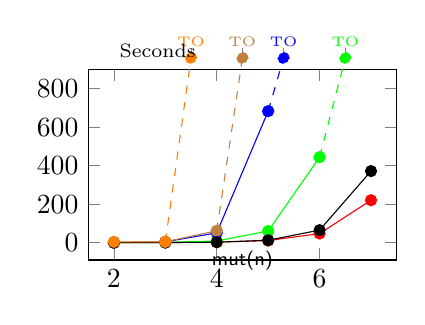
\begin{tikzpicture}
	\begin{axis}[name=Mutex,height=4cm,width=5.5cm,
		xlabel=\scriptsize{\textsf{mut(n)}},
		ylabel=\scriptsize{Seconds},
		x label style={at={(axis description cs:0.5,0.1)},anchor=north},
    	    y label style={at={(axis description cs:0.07,1.1)},anchor=west,rotate=-90},
    	%xmax=9,
		ymax=900,
		clip=false,
         %legend pos=north east
		]
    %exp2
	\addplot[color=red,mark=*] coordinates {
		(2, 0.461)
		(3, 0.877)
		(4, 2.945)
		(5, 11.05)
		(6, 47.634)
		(7, 220.863)
	};
	%exp4
	\addplot[color=green,mark=*] coordinates {
		(2, 0.483)
		(3, 1.602)
		(4, 9.032)
		(5, 60.845)
		(6, 444.691)
		%(6.5, 960) %time out
	};
	\addplot[color=green,mark=*,dashed] coordinates {		
		(6, 444.691)
		(6.5, 960) %time out
	}node[pin={[pin distance=-0.1cm]90:{\tiny{TO}}}]{};
	
	%exp8
	\addplot[color=blue,mark=*] coordinates {
		(2,0.983)
		(3,4.693)
		(4,51.233)
		(5,683.642)
		%(5.3,960) % time out
		%(7,1000)
		%(8,80.27)
		% (9,3600)
	};
	\addplot[color=blue,mark=*,dashed] coordinates {		
		(5,683.642)
		(5.3,960) % time out
		%(7,1000)
		%(8,80.27)
		% (9,3600)
	}node[pin={[pin distance=-0.1cm]90:{\tiny{TO}}}]{};
	
	%lineal10
	\addplot[color=brown,mark=*] coordinates {
		(2,0.608)
		(3,5.016)
		(4,62.034)
		%(4.5,960) % time out
		%(6,2.6)
		%(7,13.12)
		%(8,80.27)
		% (9,3600)
	};
	\addplot[color=brown,mark=*,dashed] coordinates {
		%(2,0.608)
		%(3,5.016)
		(4,62.034)
		(4.5,960) % time out
		%(6,2.6)
		%(7,13.12)
		%(8,80.27)
		% (9,3600)
	}node[pin={[pin distance=-0.1cm]90:{\tiny{TO}}}]{};
	%nocex
	\addplot[color=black,mark=*] coordinates {
		(2,0.348)
		(3,0.75)
		(4,2.679)
		(5,12.971)
		(6,65.403)
		(7,372.247)
		%(8,80.27)
		% (9,3600)
	};
	%psketch
	\addplot[color=orange,mark=*] coordinates {
		(2,4.62)
		(3,4.664)
		%(3.5,960)
		%(5,12.971)
		%(6,65.403)
		%(7,372.247)
		%(8,80.27)
		% (9,3600)
	};
	\addplot[color=orange,mark=*,dashed] coordinates {
		%(2,4.62)
		(3,4.664)
		(3.5,960)
		%(5,12.971)
		%(6,65.403)
		%(7,372.247)
		%(8,80.27)
		% (9,3600)
	}node[pin={[pin distance=-0.1cm]90:{\tiny{TO}}}]{};
	
	 %\addplot[color=black,mark=*] coordinates {
	% 	(9,3600)
	% } node[pin=180:{TO}]{};
	% \addplot[color=blue,dashed] coordinates {
	% 	(8,300)
	% 	(9,200)
	 %} node[pin=300:{TO}]{};
	%\addplot[color=green,mark=*,dashed] coordinates {
	%	(7,310)
		%(9, 107)
	%	} node[pin=180:{TO}]{};
	%\legend{exp2, exp4,exp8,lineal10,nocex}
	%\node[above right] at (rel axis cs:1, 1.1) {Time out:};
	%\node[above right] at (rel axis cs:0, 1) {\;\;\scriptsize{T.O:}};
	\end{axis}
\end{tikzpicture}
\label{fig:comparison}
% PHILOSOPHERS
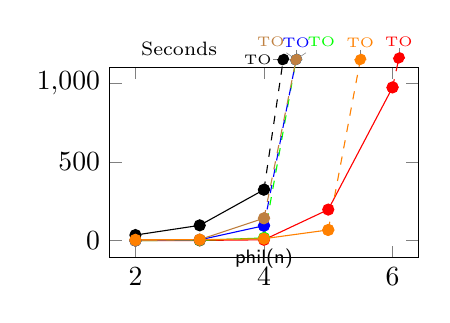
\begin{tikzpicture}
	\begin{axis}[name=Philosophers,height=4cm,width=5.5cm,
		xlabel=\scriptsize{\textsf{phil(n)}},
		ylabel=\scriptsize{Seconds},
		ymax=1100,
		clip=false,
		x label style={at={(axis description cs:0.5,0.1)},anchor=north},
    	y label style={at={(axis description cs:0.07,1.1)},anchor=west,rotate=-90},
		legend pos=north west]
    %exp2
	\addplot[color=red,mark=*] coordinates {
		(2,1.117)
		(3, 1.808)
		(4, 5.987)
		(5,197.652)
		(6,973.321)
		%(6.1,1160)
	};
	\addplot[color=red,mark=*,dashed] coordinates {
		(6,973.321)
		(6.1,1160)
	}node[pin={[pin distance=-0.1cm]90:{\tiny{TO}}}]{};
	%exp4
	\addplot[color=green,mark=*] coordinates {
		(2,1.253)
		(3, 2.765)
		(4, 17.661)
		%(4.5,1150)
		%(6,973.321)
		%(7,1000)
	};
	\addplot[color=green,mark=*,dashed] coordinates {
		(4, 17.661)
		(4.5,1150)
		%(6,973.321)
		%(7,1000)
	}node[pin={[pin distance=-0.1cm]60:{\tiny{TO}}}]{};
	
	%exp8
	\addplot[color=blue,mark=*] coordinates {
		(2,1.37)
		(3,5.552)
		(4,95.327)
		%(4.5,1150)
	     % (8,3600)
	};
	\addplot[color=blue,mark=*,dashed] coordinates {
		(4,95.327)
		(4.5,1150)
	     % (8,3600)
	}node[pin={[pin distance=-0.1cm]90:{\tiny{TO}}}]{};
	%lineal10
	\addplot[color=brown,mark=*] coordinates {
		(2,1.37)
		(3,7.264)
		(4,142.584)
		%(4.5,1150)
	     % (8,3600)
	};
	\addplot[color=brown,mark=*,dashed] coordinates {
		(4,142.584)
		(4.5,1150)
	     % (8,3600)
	}node[pin={[pin distance=-0.1cm]120:{\tiny{TO}}}]{};
	%nocex
	\addplot[color=black,mark=*] coordinates {
		(2,35.998)
		(3,97.636)
		(4,324)
		%(4.3,1150)
	     % (8,3600)
	};
	\addplot[color=black,mark=*,dashed] coordinates {
		(4,324)
		(4.3,1150)
	     % (8,3600)
	}node[pin={[pin distance=-0.1cm]180:{\tiny{TO}}}]{};
	%pskecth
	\addplot[color=orange,mark=*] coordinates {
		(2,5.916)
		(3,6.273)
		(4,12.845)%TO
		 (5,  68.5)
	     %(5.5,1150)
	};
	\addplot[color=orange,mark=*, dashed] coordinates {
		 (5,  68.5)
	     (5.5,1150)
	}node[pin={[pin distance=-0.1cm]90:{\tiny{TO}}}]{};
%\legend{exp2, PSketch}
     %\node[above right] at (rel axis cs:0, 1) {\;\;\scriptsize{T.O.:}};
	\end{axis}
\end{tikzpicture}
% BARRIER
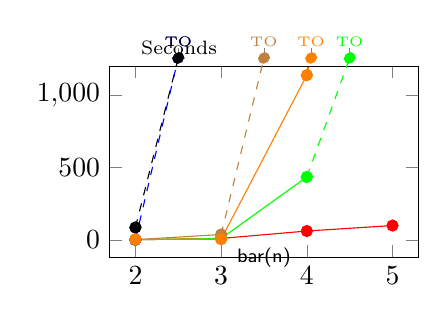
\begin{tikzpicture}
	\begin{axis}[name=SenseBarrier,height=4cm,width=5.5cm,
		xlabel=\scriptsize{\textsf{bar(n)}},
		ylabel=\scriptsize{Seconds},
		ymax=1200,
		clip=false,
		x label style={at={(axis description cs:0.5,0.1)},anchor=north},
    	y label style={at={(axis description cs:0.07,1.1)},anchor=west,rotate=-90},
		legend pos=north west]
    %exp2
	\addplot[color=red,mark=*] coordinates {
	    
		(2,1.535)
		(3, 10.761)
		(4, 62.111)
		(5,100)
		
	};
	%exp4
	\addplot[color=green,mark=*] coordinates {
	
		(2,1.672)
		(3, 10.569)
		(4, 436.365)
		%(4.5,1260) % TO
		%(6,973.321)
		%(7,1000)
	};
	\addplot[color=green,mark=*,dashed] coordinates {
		(4, 436.365)
		(4.5,1260) % TO
		%(6,973.321)
		%(7,1000)
	}node[pin={[pin distance=-0.1cm]90:{\tiny{TO}}}]{};
	
	%exp8
	\addplot[color=blue,mark=*] coordinates {
		(2,2.304)
	%	(2.5,1260)%TO
		%(4,95.327)
		%(5,1150)
	     % (8,3600)
	};
	\addplot[color=blue,mark=*,dashed] coordinates {
		(2,2.304)
		(2.5,1260)%TO
		%(4,95.327)
		%(5,1150)
	     % (8,3600)
	}node[pin={[pin distance=-0.1cm]90:{\tiny{TO}}}]{};
	%lineal10
	\addplot[color=brown,mark=*] coordinates {
	
		(2,2.362)
		(3,37.755)
		%(3.5,1260) % TO
		%(5,1150)
	     % (8,3600)
	};
	\addplot[color=brown,mark=*,dashed] coordinates {
	
		%(2,2.362)
		(3,37.755)
		(3.5,1260) % TO
		%(5,1150)
	     % (8,3600)
	}node[pin={[pin distance=-0.1cm]90:{\tiny{TO}}}]{};
	%nocex
	\addplot[color=black,mark=*] coordinates {
	   
		(2,86.916)
		%(2.5,1260)% TO
		%(4,324)
		%(4.3,1150)
	     % (8,3600)
	};
	\addplot[color=black,mark=*,dashed] coordinates {
	   
		(2,86.916)
		(2.5,1260)% TO
		%(4,324)
		%(4.3,1150)
	     % (8,3600)
	}node[pin={[pin distance=-0.1cm]90:{\tiny{TO}}}]{};
	%PSkecth
	\addplot[color=orange,mark=*] coordinates {
		(2,4.233)
		(3, 5.31)% TO
		(4,1140.9)
		%(4.05,1260)
	     % (8,3600)
	};
	\addplot[color=orange,mark=*,dashed] coordinates {
		(4,1140.9)
		(4.05,1260)
	     % (8,3600)
	}node[pin={[pin distance=-0.1cm]90:{\tiny{TO}}}]{};
%\legend{exp2, PSketch}
    %\node[above right] at (rel axis cs:0, 1) {\;\;\scriptsize{T.O.:}};
	\end{axis}
\end{tikzpicture}

% READERS & WRITERS
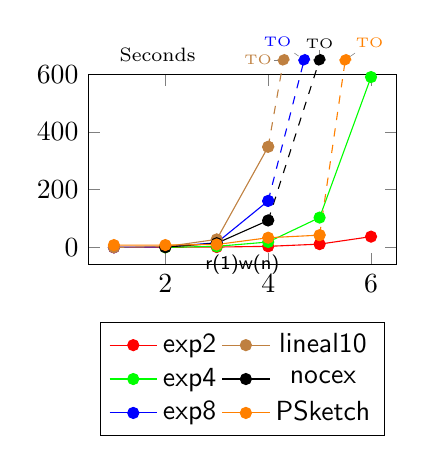
\begin{tikzpicture}
	\begin{axis}[name=Readers and Writers,height=4cm,width=5.5cm,
		xlabel=\scriptsize{\textsf{r(1)w(n)}},
		ylabel=\scriptsize{Seconds},
		x label style={at={(axis description cs:0.5,0.1)},anchor=north},
    	y label style={at={(axis description cs:0.07,1.1)},anchor=west,rotate=-90},
    	ymax=600,
		clip=false,
		legend style={at={(0.5,-0.3)},anchor=north,legend  columns =3, transpose legend}]
    % exp2
     \addlegendimage{red, line legend, mark=*} % or mark=none?
    \addlegendentry{\textsf{exp2}}
    \addlegendimage{green, line legend, , mark=*} % or mark=none?
    \addlegendentry{\textsf{exp4}}
    \addlegendimage{blue, line legend, , mark=*} % or mark=none?
    \addlegendentry{\textsf{exp8}}
    \addlegendimage{brown, line legend, , mark=*} % or mark=none?
    \addlegendentry{\textsf{lineal10}}
    \addlegendimage{black,,line legend,  mark=*} % or mark=none?
    \addlegendentry{\textsf{nocex}}
    \addlegendimage{orange,,line legend,  mark=*} % or mark=none?
    \addlegendentry{\textsf{PSketch}}
	\addplot[color=red,mark=*] coordinates {
		(1,0.492)
		(2,0.813)
		(3,1.603)
		(4,4.069)
		(5,11.705)
		(6,37.703)
	};
	% exp4
	\addplot[color=green,mark=*] coordinates {
		%(1,0.439)
		(2,0.442)
		(3,4.055)
		(4,19.064)
		(5,103.635)
		(6,590.277)
	};
	% exp8
	\addplot[color=blue,mark=*] coordinates {
		(1,0.625)
		(2,2.247)
		(3,16.51)
		(4,161.499)
		%(5,600) %TO
	};
	\addplot[color=blue,mark=*,dashed] coordinates {
		(4,161.499)
		(4.7,650) %TO
	}node[pin={[pin distance=-0.1cm]130:{\tiny{TO}}}]{};
	%lineal10
	\addplot[color=brown,mark=*] coordinates {
		(1,0.654)
		(2,2.892)
		(3,28.208)
		(4,348.931)
		%(4.3,660) %TO
	};
	\addplot[color=brown,mark=*,dashed] coordinates {
		(4,348.931)
		(4.3,650) %TO
	}node[pin={[pin distance=-0.1cm]180:{\tiny{TO}}}]{};
	\addplot[color=black,mark=*] coordinates {
		%(1,0.511)
		(2,1.344)
		(3,14.807)
		(4,93.844)
		%(5,600) %TO
	};
	\addplot[color=black,mark=*,dashed] coordinates {
		%(1,0.511)
		(4,93.844)
		(5,650) %TO
	}node[pin={[pin distance=-0.1cm]90:{\tiny{TO}}}]{};
	
	%PSketch
	\addplot[color=orange,mark=*] coordinates {
		(1,8.465)
		(2,8.483)
		(3,10.463)
		(4,33.898)
		(5,42.824)
		%(6,600)%TO
	};
	\addplot[color=orange,mark=*,dashed] coordinates {
		(5,42.824)
		(5.5,650)%TO
	}node[pin={[pin distance=-0.1cm]70:{\tiny{TO}}}]{};
   %\legend{exp2,exp4,exp8,lineal10,nocex,psketch}
    %\node[above right] at (rel axis cs:0, 1) {\;\;\scriptsize{T.O.:}};
	\end{axis}
\end{tikzpicture}
\vspace{0.4cm}
\captionof{figure}{Comparison between \\ \textsf{exp2}, \textsf{exp4}, \textsf{exp8},  \textsf{lineal10},  \textsf{nocex}, \\ and {\PSketch}.}
\label{fig:examples-plot}
\end{minipage}
\end{tabular}
\vspace{-0.5cm}
\end{table}
}
%{\scriptsize
%\begin{table}[!ht]
%\begin{tabular}{l l}
%\begin{minipage}{0.67\linewidth}
%    \centering
%    \begin{tabular}{|l|l|l|l|l|l|l|l|}
%    \hline
%        Ex. & Sc. & L.Time & G.Time & It. & R.St. & T.St. & Res. \\ \hline
%        Arb2 & 12 & 0.814 &  1.322 & 7 & $2^{2.32}$  & $2^{12}$ & F \\ \hline
%        Arb3 & 12 & 0.728 & 2.11 & 16 & $2^4$ & $2^18$ & F \\ \hline
%        Arb4 & 12 & 0.854 & 4.303 & 16 & $2^{5.24}$ & $2^{24}$ & F \\ \hline
%        Arb5 & 12 & 0.976 & 12.54 & 16 & $2^{6.35}$ & $2^{30}$ & F \\ \hline
%        Arb6 & 12 & 1.134 & 52.344 & 16 & $2^{7.40}$ & $2^{36}$ & F \\ \hline
%        FArb2 & 12 & 0.552 & 1.164 & 8 & $2^{2.58}$ & $2^{12}$ & F \\ \hline
%        FArb3 & 12 & 0.75 & 2.97 & 20 & $2^{3.45}$ & $2^{18}$ & F \\ \hline
%        FArb4 & 12 & 0.935 & 15.602 & 56 & $2^{4.39}$ & $2^{24}$ & F \\ \hline
%        FArb5 & 12 & 1.232 & 85.933 & 164 & $2^{5.35}$ & $2^{30}$ & F \\ \hline
%        FArb6 & 12 & 2.034 & 1004.49 & 857 & - & - & NF\\ \hline
%        FArb2 & 12 & 0.662 & 1.166 & 8 & $2^{2.80}$ & $2^{12}$ & F\\ \hline
%        PArb3 & 12 & 0.714 & 2.277 & 20 & $2^{3.45}$ & $2^{18}$ & F \\ \hline
%        PArb4 & 12 & 0.886 & 8.593 & 56 & $2^{4.39}$ & $2^{24}$ & F\\ \hline
%        PArb5 & 12 & 1.092 & 54.25 & 164 & $2^{5.35}$ & $2^{30}$ & F \\ \hline
%        PArb6 & 12 &1.324 & 700.731 & 488 & $2^{6.33}$ & $2^{36}$ & F \\ \hline
%    \end{tabular}
%\caption{Results for the Arbiter examples.}\label{tab:results-arbiter}
%\end{minipage}
%\begin{minipage}{0.50\linewidth}
%\centering
%\begin{tikzpicture}
%	\begin{axis}[name=Arbiter,height=4cm,width=5.5cm,
%		xlabel=\scriptsize{Arbiter(n)},
%		ylabel=\scriptsize{Seconds},
%		x label style={at={(axis description cs:0.5,0.1)},anchor=north},
%    	y label style={at={(axis description cs:0.07,1.1)},anchor=west,rotate=-90},
%    	ymax=75,
%		clip=false,
%		legend pos=north west]
%    % exp2
%	\addplot[color=red,mark=*] coordinates {
%		(2,0.768)
%		(3,1.563)
%		(4,2.175)
%		(5,3.768)
%		(6,9.172)
%		%(6,37.703)
%	};
%	% exp4
%	\addplot[color=green,mark=*] coordinates {
%		(2,0.78)
%		(3,1.687)
%		(4,3.085)
%		(5,6.985)
%		(6,19.659)
%	};
%	% exp8
%	\addplot[color=blue,mark=*] coordinates {
%		(2,0.67)
%		(3,2.132)
%		(4,4)
%		(5,10.624)
%		(6, 35.653) 
%	};
%	%lineal10
%	\addplot[color=brown,mark=*] coordinates {
%		(2,0.972)
%		(3,3.359)
%		(4,7.829)
%		(5,16.491)
%		(6,54.652)
%	};
%	%Party
%	\addplot[color=pink,mark=*] coordinates {
%		(2,0.63)
%		(3,1.18)
%		(4,2.82)
%		(5,6.12)
%		(6,12.43)
%	};
%	%nocex
%	%\addplot[color=black,mark=x] coordinates {
%	%	(1,0.511)
%	%	(2,1.344)
%	%	(3,14.807)
%	%	(4,93.844)
%	%	(5,600) %TO
%	%};
%	
%%\legend{exp2,exp4,exp8,lineal10,nocex}
%    \node[above right] at (rel axis cs:0, 1) {\;\;\scriptsize{Time out:}};
%	\end{axis}
%\end{tikzpicture}
%%Full Arbiter
%\begin{tikzpicture}
%	\begin{axis}[name=FullArbiter,height=4cm,width=5.5cm,
%		xlabel=\scriptsize{FullArbiter(n)},
%		ylabel=\scriptsize{Seconds},
%		x label style={at={(axis description cs:0.5,0.1)},anchor=north},
%    	y label style={at={(axis description cs:0.07,1.1)},anchor=west,rotate=-90},
%    	ymax=1200,
%		clip=false,
%		legend pos=north west]
%    % exp2
%	\addplot[color=red,mark=*] coordinates {
%		(2,1.164)
%		(3,2.97)
%		(4,15.609)
%		(5,85.933)
%		(6,1004.49)
%		%(6,37.703)
%	};
%	% exp4
%	\addplot[color=green,mark=*] coordinates {
%		(2,0.8)
%		(3,1.466)
%		(4,3.457)
%		(5,10.8)
%		(6,66.433)
%	};
%	% exp8
%	\addplot[color=blue,mark=*] coordinates {
%		(2,0.83)
%		(3,1.507)
%		(4,3.562)
%		(5,12.345)
%		(6, 69.144) %TO
%	};
%	%lineal10
%	\addplot[color=brown,mark=*] coordinates {
%		(2,2.024)
%		(3,19.822)
%		(4,298.955)
%		(5,1200)%TO
%	};
%	\addplot[color=pink,mark=*] coordinates {
%		(2,0.68)
%		(3,1.43)
%		(4,4.078)
%		(5,8.85)
%		(6,32.73)
%	};
%	%nocex
%	%\addplot[color=black,mark=x] coordinates {
%	%	(1,0.511)
%	%	(2,1.344)
%	%	(3,14.807)
%	%	(4,93.844)
%	%	(5,600) %TO
%	%};
%%\legend{exp2,exp4,exp8,lineal10,nocex}
%    \node[above right] at (rel axis cs:0, 1) {\;\;\scriptsize{Time out:}};
%	\end{axis}
%\end{tikzpicture}
%%PNUELIARBITER
%\begin{tikzpicture}
%	\begin{axis}[name=PnueliArbiter,height=4cm,width=5.5cm,
%		xlabel=\scriptsize{PnueliArbiter(n)},
%		ylabel=\scriptsize{Seconds},
%		x label style={at={(axis description cs:0.5,0.1)},anchor=north},
%    	y label style={at={(axis description cs:0.07,1.1)},anchor=west,rotate=-90},
%    	ymax=1400,
%		clip=false,
%		legend style={at={(0.2,-0.5)},anchor=north}]
%    % exp2
%	\addplot[color=red,mark=*] coordinates {
%		(2,1.168)
%		(3,2.277)
%		(4,8.593)
%		(5,54.25)
%		(6,1362.85) % TO
%		%(6,37.703)
%	};
%	% exp4
%	\addplot[color=green,mark=*] coordinates {
%		(2,0.676)
%		(3,1.146)
%		(4,2.355)
%		(5,11.6)
%		(6,66.433) 
%	};
%	% exp8
%	\addplot[color=blue,mark=*] coordinates {
%		(2,0.707)
%		(3,1.242)
%		(4,2.433)
%		(5,12.173)
%		(6, 65.155) %TO
%	};
%	%lineal10
%	\addplot[color=brown,mark=*] coordinates {
%		(2,0.69)
%		(3,1.162)
%		(4,2.408)
%		(5,11.836)
%		(6,59.299)
%	};
%	%nocex
%	%\addplot[color=black,mark=x] coordinates {
%	%	(1,0.511)
%	%	(2,1.344)
%	%	(3,14.807)
%	%	(4,93.844)
%	%	(5,600) %TO
%	%};
%	%party
%	\addplot[color=pink,mark=*] coordinates {
%		(2,0.69)
%		(3,1.162)
%		(4,2.408)
%		(5,11.836)
%		(6,1400)
%	};
%\legend{exp2,exp4,exp8,lineal10,nocex}
%    \node[above right] at (rel axis cs:0, 1) {\;\;\scriptsize{Time out:}};
%	\end{axis}
%\end{tikzpicture}
%\end{minipage}
%\end{tabular}
%\end{table}
%}

%\begin{figure}[hbt!]
%\begin{tabular}{l l}
%\begin{minipage}{0.48\linewidth}
%\centering
%%MUTEX
%\begin{tikzpicture}
%	\begin{axis}[name=Mutex,height=4cm,width=5.5cm,
%		xlabel=\scriptsize{Mutex(n)},
%		ylabel=\scriptsize{Seconds},
%		x label style={at={(axis description cs:0.5,0.1)},anchor=north},
%    	    y label style={at={(axis description cs:0.07,1.1)},anchor=west,rotate=-90},
%    	%xmax=9,
%		ymax=900,
%		clip=false,
%         %legend pos=north east
%		]
%    %exp2
%	\addplot[color=red,mark=*] coordinates {
%		(2, 0.461)
%		(3, 0.877)
%		(4, 2.945)
%		(5, 11.05)
%		(6, 47.634)
%		(7, 220.863)
%	};
%	%exp4
%	\addplot[color=green,mark=*] coordinates {
%		(2, 0.483)
%		(3, 1.602)
%		(4, 9.032)
%		(5, 60.845)
%		(6, 444.691)
%		(7, 900) %time out
%	};
%	%exp8
%	\addplot[color=blue,mark=*] coordinates {
%		(2,0.983)
%		(3,4.693)
%		(4,51.233)
%		(5,683.642)
%		(5.3,900) % time out
%		%(7,1000)
%		%(8,80.27)
%		% (9,3600)
%	};
%	%lineal10
%	\addplot[color=brown,mark=*] coordinates {
%		(2,0.608)
%		(3,5.016)
%		(4,62.034)
%		(5,900) % time out
%		%(6,2.6)
%		%(7,13.12)
%		%(8,80.27)
%		% (9,3600)
%	};
%	%nocex
%	\addplot[color=black,mark=*] coordinates {
%		(2,0.348)
%		(3,0.75)
%		(4,2.679)
%		(5,12.971)
%		(6,65.403)
%		(7,372.247)
%		%(8,80.27)
%		% (9,3600)
%	};
%	 %\addplot[color=black,mark=*] coordinates {
%	% 	(9,3600)
%	% } node[pin=180:{TO}]{};
%	% \addplot[color=blue,dashed] coordinates {
%	% 	(8,300)
%	% 	(9,200)
%	 %} node[pin=300:{TO}]{};
%	%\addplot[color=green,mark=*,dashed] coordinates {
%	%	(7,310)
%		%(9, 107)
%	%	} node[pin=180:{TO}]{};
%	%\legend{exp2, exp4,exp8,lineal10,nocex}
%	%\node[above right] at (rel axis cs:1, 1.1) {Time out:};
%	\node[above right] at (rel axis cs:0, 1) {\;\;\scriptsize{Time out:}};
%	\end{axis}
%\end{tikzpicture}
%\label{fig:comparison}
%% PHILOSOPHERS
%\begin{tikzpicture}
%	\begin{axis}[name=Philosophers,height=4cm,width=5.5cm,
%		xlabel=\scriptsize{Phils(n)},
%		ylabel=\scriptsize{Seconds},
%		ymax=1100,
%		clip=false,
%		x label style={at={(axis description cs:0.5,0.1)},anchor=north},
%    	y label style={at={(axis description cs:0.07,1.1)},anchor=west,rotate=-90},
%		legend pos=north west]
%    %exp2
%	\addplot[color=red,mark=*] coordinates {
%		(2,1.117)
%		(3, 1.808)
%		(4, 5.987)
%		(5,197.652)
%		(6,973.321)
%		(6.1,1100)
%	};
%	%exp4
%	\addplot[color=green,mark=*] coordinates {
%		(2,1.253)
%		(3, 2.765)
%		(4, 17.661)
%		(5,1100)
%		%(6,973.321)
%		%(7,1000)
%	};
%	%exp8
%	\addplot[color=blue,mark=*] coordinates {
%		(2,1.37)
%		(3,5.552)
%		(4,95.327)
%		(5,1100)
%	     % (8,3600)
%	};
%	%lineal10
%	\addplot[color=brown,mark=*] coordinates {
%		(2,1.37)
%		(3,7.264)
%		(4,142.584)
%		(5,1100)
%	     % (8,3600)
%	};
%	%nocex
%	\addplot[color=black,mark=*] coordinates {
%		(2,35.998)
%		(3,97.636)
%		(4,324)
%		(4.3,1100)
%	     % (8,3600)
%	};
%%\legend{exp2, PSketch}
%     \node[above right] at (rel axis cs:0, 1) {\;\;\scriptsize{Time out:}};
%	\end{axis}
%\end{tikzpicture}
%% BARRIER
%\begin{tikzpicture}
%	\begin{axis}[name=SenseBarrier,height=4cm,width=5.5cm,
%		xlabel=\scriptsize{SenseBarrier(n)},
%		ylabel=\scriptsize{Seconds},
%		ymax=500,
%		clip=false,
%		x label style={at={(axis description cs:0.5,0.1)},anchor=north},
%    	y label style={at={(axis description cs:0.07,1.1)},anchor=west,rotate=-90},
%		legend pos=north west]
%    %exp2
%	\addplot[color=red,mark=*] coordinates {
%	    
%		(2,1.535)
%		(3, 10.761)
%		(4, 62.111)
%		(5,100)
%		
%	};
%	%exp4
%	\addplot[color=green,mark=*] coordinates {
%	
%		(2,1.672)
%		(3, 10.569)
%		(4, 436.365)
%		(4.1,500) % TO
%		%(6,973.321)
%		%(7,1000)
%	};
%	%exp8
%	\addplot[color=blue,mark=*] coordinates {
%	
%		(2,2.304)
%		(3,500)%TO
%		%(4,95.327)
%		%(5,1150)
%	     % (8,3600)
%	};
%	%lineal10
%	\addplot[color=brown,mark=*] coordinates {
%	
%		(2,2.362)
%		(3,37.755)
%		(4,500) % TO
%		%(5,1150)
%	     % (8,3600)
%	};
%	%nocex
%	\addplot[color=black,mark=*] coordinates {
%	   
%		(2,86.916)
%		(2.5,500)% TO
%		%(4,324)
%		%(4.3,1150)
%	     % (8,3600)
%	};
%%\legend{exp2, PSketch}
%    \node[above right] at (rel axis cs:0, 1) {\;\;\scriptsize{Time out:}};
%	\end{axis}
%\end{tikzpicture}
%
%% READERS & WRITERS
%\begin{tikzpicture}
%	\begin{axis}[name=Readers and Writers,height=4cm,width=5.5cm,
%		xlabel=\scriptsize{RW(1,n)},
%		ylabel=\scriptsize{Seconds},
%		x label style={at={(axis description cs:0.5,0.1)},anchor=north},
%    	y label style={at={(axis description cs:0.07,1.1)},anchor=west,rotate=-90},
%    	ymax=600,
%		clip=false,
%		legend pos=north west]
%    % exp2
%	\addplot[color=red,mark=*] coordinates {
%		(1,0.492)
%		(2,0.813)
%		(3,1.603)
%		(4,4.069)
%		(5,11.705)
%		(6,37.703)
%	};
%	% exp4
%	\addplot[color=green,mark=*] coordinates {
%		(1,0.439)
%		(2,0.442)
%		(3,4.055)
%		(4,19.064)
%		(5,103.635)
%		(6,590.277)
%	};
%	% exp8
%	\addplot[color=blue,mark=*] coordinates {
%		(1,0.625)
%		(2,2.247)
%		(3,16.51)
%		(4,161.499)
%		(5,600) %TO
%	};
%	%lineal10
%	\addplot[color=brown,mark=*] coordinates {
%		(1,0.654)
%		(2,2.892)
%		(3,28.208)
%		(4,348.931)
%		(4.3,600) %TO
%	};
%	\addplot[color=black,mark=*] coordinates {
%		(1,0.511)
%		(2,1.344)
%		(3,14.807)
%		(4,93.844)
%		(5,600) %TO
%	};
%
%%\legend{exp2,exp4,exp8,lineal10,nocex}
%    \node[above right] at (rel axis cs:0, 1) {\;\;\scriptsize{Time out:}};
%	\end{axis}
%\end{tikzpicture}
%\end{minipage}
%%\captionof{figure}{Comparison for exp2, exp4, exp8, lineal10, and nocex.}
%&
%%%% ARBITER EXAMPLES
%%Arbiter
%\begin{minipage}{0.48\linewidth}
%\centering
%\begin{tikzpicture}
%	\begin{axis}[name=Arbiter,height=4cm,width=5.5cm,
%		xlabel=\scriptsize{Arbiter(n)},
%		ylabel=\scriptsize{Seconds},
%		x label style={at={(axis description cs:0.5,0.1)},anchor=north},
%    	y label style={at={(axis description cs:0.07,1.1)},anchor=west,rotate=-90},
%    	ymax=75,
%		clip=false,
%		legend pos=north west]
%    % exp2
%	\addplot[color=red,mark=*] coordinates {
%		(2,0.768)
%		(3,1.563)
%		(4,2.175)
%		(5,3.768)
%		(6,9.172)
%		%(6,37.703)
%	};
%	% exp4
%	\addplot[color=green,mark=*] coordinates {
%		(2,0.78)
%		(3,1.687)
%		(4,3.085)
%		(5,6.985)
%		(6,19.659)
%	};
%	% exp8
%	\addplot[color=blue,mark=*] coordinates {
%		(2,0.67)
%		(3,2.132)
%		(4,4)
%		(5,10.624)
%		(6, 35.653) 
%	};
%	%lineal10
%	\addplot[color=brown,mark=*] coordinates {
%		(2,0.972)
%		(3,3.359)
%		(4,7.829)
%		(5,16.491)
%		(6,54.652)
%	};
%	%Party
%	\addplot[color=pink,mark=*] coordinates {
%		(2,0.63)
%		(3,1.18)
%		(4,2.82)
%		(5,6.12)
%		(6,12.43)
%	};
%	%nocex
%	%\addplot[color=black,mark=x] coordinates {
%	%	(1,0.511)
%	%	(2,1.344)
%	%	(3,14.807)
%	%	(4,93.844)
%	%	(5,600) %TO
%	%};
%	
%%\legend{exp2,exp4,exp8,lineal10,nocex}
%    \node[above right] at (rel axis cs:0, 1) {\;\;\scriptsize{Time out:}};
%	\end{axis}
%\end{tikzpicture}
%%Full Arbiter
%\begin{tikzpicture}
%	\begin{axis}[name=FullArbiter,height=4cm,width=5.5cm,
%		xlabel=\scriptsize{FullArbiter(n)},
%		ylabel=\scriptsize{Seconds},
%		x label style={at={(axis description cs:0.5,0.1)},anchor=north},
%    	y label style={at={(axis description cs:0.07,1.1)},anchor=west,rotate=-90},
%    	ymax=1200,
%		clip=false,
%		legend pos=north west]
%    % exp2
%	\addplot[color=red,mark=*] coordinates {
%		(2,1.164)
%		(3,2.97)
%		(4,15.609)
%		(5,85.933)
%		(6,1004.49)
%		%(6,37.703)
%	};
%	% exp4
%	\addplot[color=green,mark=*] coordinates {
%		(2,0.8)
%		(3,1.466)
%		(4,3.457)
%		(5,10.8)
%		(6,66.433)
%	};
%	% exp8
%	\addplot[color=blue,mark=*] coordinates {
%		(2,0.83)
%		(3,1.507)
%		(4,3.562)
%		(5,12.345)
%		(6, 69.144) %TO
%	};
%	%lineal10
%	\addplot[color=brown,mark=*] coordinates {
%		(2,2.024)
%		(3,19.822)
%		(4,298.955)
%		(5,1200)%TO
%	};
%	\addplot[color=pink,mark=*] coordinates {
%		(2,0.68)
%		(3,1.43)
%		(4,4.078)
%		(5,8.85)
%		(6,32.73)
%	};
%	%nocex
%	%\addplot[color=black,mark=x] coordinates {
%	%	(1,0.511)
%	%	(2,1.344)
%	%	(3,14.807)
%	%	(4,93.844)
%	%	(5,600) %TO
%	%};
%%\legend{exp2,exp4,exp8,lineal10,nocex}
%    \node[above right] at (rel axis cs:0, 1) {\;\;\scriptsize{Time out:}};
%	\end{axis}
%\end{tikzpicture}
%%PNUELIARBITER
%\begin{tikzpicture}
%	\begin{axis}[name=PnueliArbiter,height=4cm,width=5.5cm,
%		xlabel=\scriptsize{PnueliArbiter(n)},
%		ylabel=\scriptsize{Seconds},
%		x label style={at={(axis description cs:0.5,0.1)},anchor=north},
%    	y label style={at={(axis description cs:0.07,1.1)},anchor=west,rotate=-90},
%    	ymax=1400,
%		clip=false,
%		legend style={at={(0.2,-0.5)},anchor=north}]
%    % exp2
%	\addplot[color=red,mark=*] coordinates {
%		(2,1.168)
%		(3,2.277)
%		(4,8.593)
%		(5,54.25)
%		(6,1362.85) % TO
%		%(6,37.703)
%	};
%	% exp4
%	\addplot[color=green,mark=*] coordinates {
%		(2,0.676)
%		(3,1.146)
%		(4,2.355)
%		(5,11.6)
%		(6,66.433) 
%	};
%	% exp8
%	\addplot[color=blue,mark=*] coordinates {
%		(2,0.707)
%		(3,1.242)
%		(4,2.433)
%		(5,12.173)
%		(6, 65.155) %TO
%	};
%	%lineal10
%	\addplot[color=brown,mark=*] coordinates {
%		(2,0.69)
%		(3,1.162)
%		(4,2.408)
%		(5,11.836)
%		(6,59.299)
%	};
%	%nocex
%	%\addplot[color=black,mark=x] coordinates {
%	%	(1,0.511)
%	%	(2,1.344)
%	%	(3,14.807)
%	%	(4,93.844)
%	%	(5,600) %TO
%	%};
%	%party
%	\addplot[color=pink,mark=*] coordinates {
%		(2,0.69)
%		(3,1.162)
%		(4,2.408)
%		(5,11.836)
%		(6,1400)
%	};
%\legend{exp2,exp4,exp8,lineal10,nocex}
%    \node[above right] at (rel axis cs:0, 1) {\;\;\scriptsize{Time out:}};
%	\end{axis}
%\end{tikzpicture}
%\vspace{1.3cm}
%
%%\captionof{figure}{Comparison with Party Tool.}
%\label{fig:comparison}
%\end{minipage}
%\end{tabular}
%\end{figure}
We evaluate our approach around the following research questions: 
\begin{description}
\item[RQ1] \emph{How effective/efficient is our synthesis approach?}
\item[RQ2] \emph{How good is the counterexample-guided search for speeding up the synthesis method?}
\item[RQ3] \emph{How do the selected bounds affect the synthesis method?}
\item[RQ4] \emph{How does our approach compare with related approaches?}
\end{description}
To answer these questions,  we implemented Alg.~\ref{alg:improved_alg} in a prototype tool, it uses the \textsf{Alloy Analyzer}~\cite{AlloyBook} for obtaining instances of specifications, and {\NuSMV}~\cite{Cimatti+2002} for model checking the candidates.  We evaluate our approach on eight  examples of distributed algorithms: the dining philosophers (\textsf{phil})~\cite{Dijkstra71} (our running example), Mutex (\textsf{mut})~\cite{Fokkink13},  Readers and Writers (\textsf{rw})~\cite{Fokkink13}, the generalized version of Peterson's algorithm (\textsf{pet})~\cite{Fokkink13},   and the combined-tree Barrier protocol (\textsf{bar})~\cite{Fokkink13}.  Furthermore,  we  also encoded the arbiter examples presented in \cite{Party,Piterman+2006}: a simple arbiter (\textsf{arb}), a full arbiter (\textsf{farb}), and the Pnueli arbiter (\textsf{parb}). These case studies assume a distributed token ring architecture,  which we modeled using the Alloy language.  

%\cite{PhilStone}. The tool takes as input a  specification and returns, when possible, an LTS satisfying the specification, described in the \NuSMV  language.
Tables~\ref{tab:results-common} and~\ref{tab:results-arbiter}  summarize the experimental results. The experiments were conducted on an Apple M2 processor with 16GB of memory.   In these examples, we used the sequence of bounds $2,4,8,16,\dots$, named \textsf{exp2} from now on.
For each case study, we report the 
bound over the size of the processes (Sc), the maximum time needed to generate local process instances (L.Time), the total time required for synthesizing the system (T.Time), the number of times that the model checker was invoked (Its) by the synthesizer, and the final result of our synthesis algorithm:  `F' (if an implementation was found),  `N'  (if no implementation was found),  `TO'  if the example timed out, or `U'  (if the specification was found unsatisfiable by the Alloy tool).  We also report the number of reachable states (R.St.), and the total states (T.St.) of the obtained implementations, expressed as power of $2$.  For space reasons, we only include a few configurations found unsatisfiable by the solver; similar numbers can be obtained for the rest of the cases if the specifications are processed with smaller scopes. We also indicate the number of processes considered in each experiment.  For instance,  \textsf{phil(6)} indicates that we considered \textsf{6} concurrent processes (i.e., philosophers) in the dining philosophers example. In the case of Readers and Writers, 
\textsf{r(n)w(m)} means that \textsf{n} readers and \textsf{m} writers were considered.  We  have  set out a time out of 30 minutes.
\begin{wraptable}[19]{r}{.60\textwidth}
\vspace{-0.5cm}
\begin{tabular}{|l|l|l|l|l|l|l|l|}
    \hline
        Ex. & Sc. & L.Time & G.Time & It. & R.St. & T.St. & Res. \\ \hline
        \textsf{arb(2)} & 12 & 0.814 &  1.322 & 7 & $2^{2.32}$  & $2^{12}$ & F \\ \hline
        \textsf{arb(3)} & 12 & 0.728 & 2.11 & 16 & $2^4$ & $2^{18}$ & F \\ \hline
        \textsf{arb(4)} & 12 & 0.854 & 4.303 & 16 & $2^{5.24}$ & $2^{24}$ & F \\ \hline
        \textsf{arb(5)} & 12 & 0.976 & 12.54 & 16 & $2^{6.35}$ & $2^{30}$ & F \\ \hline
        \textsf{arb(6)} & 12 & 1.134 & 52.344 & 16 & $2^{7.40}$ & $2^{36}$ & F \\ \hline
        \textsf{farb(2)} & 12 & 0.552 & 1.164 & 8 & $2^{2.58}$ & $2^{12}$ & F \\ \hline
        \textsf{farb(3)} & 12 & 0.75 & 2.97 & 20 & $2^{3.45}$ & $2^{18}$ & F \\ \hline
        \textsf{farb(4)} & 12 & 0.935 & 15.602 & 56 & $2^{4.39}$ & $2^{24}$ & F \\ \hline
        \textsf{farb(5)} & 12 & 1.232 & 85.933 & 164 & $2^{5.35}$ & $2^{30}$ & F \\ \hline
        \textsf{farb(6)} & 12 & 2.034 & 672.539 & 488 & $2^{6.33}$ & $2^{36}$ & F\\ \hline
        \textsf{parb(2)} & 12 & 0.662 & 1.166 & 8 & $2^{2.80}$ & $2^{12}$ & F\\ \hline
        \textsf{parb(3)} & 12 & 0.714 & 2.277 & 20 & $2^{3.45}$ & $2^{18}$ & F \\ \hline
        \textsf{parb(4)} & 12 & 0.886 & 8.593 & 56 & $2^{4.39}$ & $2^{24}$ & F\\ \hline
        \textsf{parb(5)} & 12 & 1.092 & 54.25 & 164 & $2^{5.35}$ & $2^{30}$ & F \\ \hline
        \textsf{parb(6)} & 12 &1.324 & 700.731 & 488 & $2^{6.33}$ & $2^{36}$ & F \\ \hline
\end{tabular}
\caption{Results for the arbiter examples.}\label{tab:results-arbiter}
\end{wraptable}
%
Table \ref{tab:results-common} shows that the technique scales reasonably well for those case studies in which each process uses only a reduced number of locks and shared variables (e.g., dining philosophers, mutex and reader-writers). For the cases where the number of shared variables accessed by the processes is bigger (e.g., Peterson for $n$ processes), the technique does not scale that well. Intuitively, more shared variables imply more actions performed by the environment, which increases the size of the formula fed to the SAT solver.  We plan to investigate how to equip specifications with assumptions on the environment's behavior, to restrict the possible values of shared variables; this may simplify the SAT problem when searching for local implementations.  It is worth noting, that even though the algorithm is incomplete, we have not 
observed any ``not found'' outputs in our benchmarks. This could be due to  the set timeouts.  We leave an in-depth investigation of this as further work.

 To answer \textbf{RQ3}   we compare the results obtained with several configurations of bounds for the exploration phase, namely: \textsf{exp4} ($4,16,64,\dots$),  \textsf{exp8} ($8,64,512,\dots$),  \textsf{lineal10} ($10,20,30,\dots$), and for \textbf{RQ2} we also considered Alg.~\ref{alg:the_alg},  which does not take into account counterexamples (\textsf{nocex}).  The obtained results are depicted in Figs.\ref{fig:examples-plot} and \ref{fig:arbiter-plots}.  Note that time outs are remarked using dashed lines going out of the $y$-axis.
 In general, \textsf{exp2} behaves better than the other options,  thus it seems better to collect a few counterexamples first, and use them to improve the search.  A possible drawback of this setting is that a wrong choice of the first counterexamples may have as a consequence that no implementation is found,  i.e., one may expect that this configuration  is ``more incomplete''   than the other options. However, we have not observed this in our benchmarks.  Note that \textsf{nocex} timed out in many examples. Indeed, for the arbiter examples, \textsf{nocex} was able only to solve the examples with two processes,  taking for that more than $7000$ iterations.

\begin{wrapfigure}[31]{hr}{.40\textwidth}
\vspace{-1.5cm}
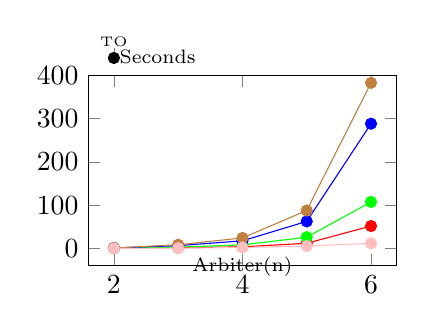
\begin{tikzpicture}
	\begin{axis}[name=Arbiter,height=4cm,width=5.5cm,
		xlabel=\scriptsize{Arbiter(n)},
		ylabel=\scriptsize{Seconds},
		x label style={at={(axis description cs:0.5,0.1)},anchor=north},
    	y label style={at={(axis description cs:0.07,1.1)},anchor=west,rotate=-90},
    	ymax=400,
		clip=false,
		legend pos=north west]
    % exp2
	\addplot[color=red,mark=*] coordinates {
		(2,1.3)
		(3,2.11)
		(4,4.3)
		(5,12.54)
		(6,52.34)
		%(6,37.703)
	};
	% exp4
	\addplot[color=green,mark=*] coordinates {
		(2,1.372)
		(3,3.545)
		(4,8.824)
		(5,26.531)
		(6,107.897)
	};
	% exp8
	\addplot[color=blue,mark=*] coordinates {
		(2,1.72)
		(3,7.022)
		(4,18.176)
		(5,63.028)
		(6, 288.419) 
	};
	%lineal10
	\addplot[color=brown,mark=*] coordinates {
		(2,1.737)
		(3,9.11)
		(4,24.866)
		(5,88.064)
		(6,382.565)
	};
	%Party
	\addplot[color=pink,mark=*] coordinates {
		(2,0.63)
		(3,1.18)
		(4,2.82)
		(5,6.12)
		(6,12.43)
	};
	%nocex
	\addplot[color=black,mark=*] coordinates {
	%	(1,0.511)
		(2,440)
	%	(3,14.807)
	%	(4,93.844)
	%	(5,600) %TO
	}node[pin={[pin distance=-0.1cm]90:{\tiny{TO}}}]{};

%\legend{exp2,exp4,exp8,lineal10,nocex}
    %\node[above right] at (rel axis cs:0, 1) {\;\;\scriptsize{T.O.:}};
	\end{axis}
\end{tikzpicture}
%Full Arbiter
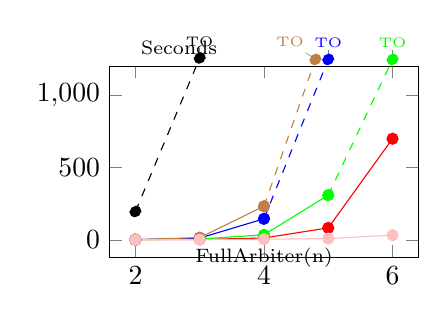
\begin{tikzpicture}
	\begin{axis}[name=FullArbiter,height=4cm,width=5.5cm,
		xlabel=\scriptsize{FullArbiter(n)},
		ylabel=\scriptsize{Seconds},
		x label style={at={(axis description cs:0.5,0.1)},anchor=north},
    	y label style={at={(axis description cs:0.07,1.1)},anchor=west,rotate=-90},
    	ymax=1200,
		clip=false,
		legend pos=north west]
    % exp2
	\addplot[color=red,mark=*] coordinates {
		(2,1.083)
		(3,2.774)
		(4,12.873)
		(5,82.981)
		(6,700.731)
		%(6,37.703)
	};
	% exp4
	\addplot[color=green,mark=*] coordinates {
		(2,1.24)
		(3,5.719)
		(4,34.7)
		(5,309.953)
	};
	\addplot[color=green,mark=*,dashed] coordinates {
		(5,309.953)
		(6,1250)
	}node[pin={[pin distance=-0.1cm]90:{\tiny{TO}}}]{};
	
	% exp8
	\addplot[color=blue,mark=*] coordinates {
		(2,1.55)
		(3,12.382)
		(4,145.86)
	};
	\addplot[color=blue,mark=*,dashed] coordinates {
		(4,145.86)
		(5,1250)
	}node[pin={[pin distance=-0.1cm]90:{\tiny{TO}}}]{};
	
	%lineal10
	\addplot[color=brown,mark=*] coordinates {
		(2,1.677)
		(3,15.45)
		(4,232.942)
		%(5,1250)%TO
	};
	\addplot[color=brown,mark=*,dashed] coordinates {
		(4,232.942)
		(4.8,1250)%TO
	}node[pin={[pin distance=-0.1cm]120:{\tiny{TO}}}]{};
	    
	%Party
	\addplot[color=pink,mark=*] coordinates {
		(2,0.68)
		(3,1.43)
		(4,4.078)
		(5,8.85)
		(6,32.73)
	};
	%nocex
	\addplot[color=black,mark=*,dashed] coordinates {
	%	(1,0.511)
		(2,196.115)
		(3,1260) % TO
	%	(4,93.844)
	%	(5,600) %TO
	}node[pin={[pin distance=-0.1cm]90:{\tiny{TO}}}]{};
	
%\legend{exp2,exp4,exp8,lineal10,nocex}
    %\node[above right] at (rel axis cs:0, 1) {\;\;\scriptsize{T.O.:}};
	\end{axis}
\end{tikzpicture}
%PNUELIARBITER
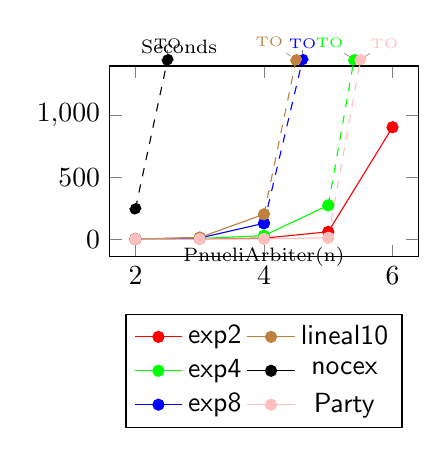
\begin{tikzpicture}
	\begin{axis}[name=PnueliArbiter,height=4cm,width=5.5cm,
		xlabel=\scriptsize{PnueliArbiter(n)},
		ylabel=\scriptsize{Seconds},
		x label style={at={(axis description cs:0.5,0.1)},anchor=north},
    	y label style={at={(axis description cs:0.07,1.1)},anchor=west,rotate=-90},
    	ymax=1400,
		clip=false,
		legend style={at={(0.5,-0.3)},anchor=north,legend  columns =3, transpose legend}]
    % exp2
     \addlegendimage{red, line legend, mark=*} % or mark=none?
    \addlegendentry{\textsf{exp2}}
    \addlegendimage{green, line legend, , mark=*} % or mark=none?
    \addlegendentry{\textsf{exp4}}
    \addlegendimage{blue, line legend, , mark=*} % or mark=none?
    \addlegendentry{\textsf{exp8}}
    \addlegendimage{brown, line legend, , mark=*} % or mark=none?
    \addlegendentry{\textsf{lineal10}}
    \addlegendimage{black,,line legend,  mark=*} % or mark=none?
    \addlegendentry{\textsf{nocex}}
    \addlegendimage{pink,line legend,  mark=*} % or mark=none?
    \addlegendentry{\textsf{Party}}
    % exp2
	\addplot[color=red,mark=*] coordinates {
		(2,1.206)
		(3,2.674)
		(4,8.639)
		(5,59.893)
		(6,905.203) % TO
		%(6,37.703)
	};
	% exp4
	\addplot[color=green,mark=*] coordinates {
		(2,1.406)
		(3,5.461)
		(4,29.063)
		(5,274.013)
	};
	\addplot[color=green,mark=*,dashed] coordinates {
		(5,274.013)
		(5.4,1450) 
	}node[pin={[pin distance=-0.1cm]110:{\tiny{TO}}}]{};
	
	% exp8
	\addplot[color=blue,mark=*] coordinates {
		(2,1.634)
		(3,9.749)
		(4,128.565)
	};
	\addplot[color=blue,mark=*,dashed] coordinates {
		(4,128.565)
		(4.6, 1450) %TO
	}node[pin={[pin distance=-0.1cm]90:{\tiny{TO}}}]{};
	%lineal10
	\addplot[color=brown,mark=*] coordinates {
		(2,1.789)
		(3,13.855)
		(4,201.653)
	};
	\addplot[color=brown,mark=*,dashed] coordinates {	
		(4,201.653)
		(4.5,1450)
	}node[pin={[pin distance=-0.1cm]130:{\tiny{TO}}}]{};
	%nocex
	\addplot[color=black,mark=*,dashed] coordinates {
	%	(1,0.511)
		(2,246.157)
	 	(2.5,1450)
	%	(4,93.844)
	%	(5,600) %TO
	}node[pin={[pin distance=-0.1cm]90:{\tiny{TO}}}]{};
	%party
	\addplot[color=pink,mark=*] coordinates {
		(2,0.69)
		(3,1.162)
		(4,2.408)
		(5,11.836)
		%(5.5,1450)
	};
	\addplot[color=pink,mark=*,dashed] coordinates {
		(5,11.836)
		(5.5,1450)
	}node[pin={[pin distance=-0.1cm]80:{\tiny{TO}}}]{};
    %\legend{exp2,exp4,exp8,lineal10,nocex,Party}
    %\node[above right] at (rel axis cs:0, 1) {\;\;\scriptsize{T.O.:}};
	\end{axis}
\end{tikzpicture}
\caption{Efficiency comparison for arbiter examples}\label{fig:arbiter-plots}
\end{wrapfigure}
To answer \textbf{RQ4} we have included in out analysis the synthesis tool {\PSketch}~\cite{Solar-Lezama+2008}, that implements a Counterexample-driven Guided Inductive Synthesis (CEGIS) algorithm to obtain code from sketched code (i.e., code annotated with ``holes''). To run {\PSketch}, we took the Dining Philosophers specification provided in~\cite{Solar-Lezama+2008}, and manually elaborated the specification for Mutex,  Readers-Writers, and the Barrier example.  The Peterson example cannot be analysed with  {\PSketch} since this tool only supports the analysis of safety properties.  For the arbiter case studies, we have compare against the tool {\Party} \cite{Party} which is a tool specifically tailored for distributed systems that use token ring architectures.

Our comparison focuses only on the time required by each technique for synthesizing the distributed solutions. The plots of Figs.~\ref{fig:examples-plot} and \ref{fig:arbiter-plots} depict the results of this comparison. In all the case studies, we notice that the efficiency of {\PSketch} is drastically affected as the number of processes to synthesize is incremented. For instance, in the dining philosophers with 6 processes, {\Sketch} timed out; in contrast, our tool was able to obtain a solution. Similarly, in the case of 1 reader and 6 writers, {\PSketch} failed in synthesizing a solution, while our approach succeeded. A similar analysis applies to Mutex.

  In the case of the tool {\Party}, for the \textsf{arb} and \textsf{farb} examples {\Party} was able to find solutions faster than \textsf{exp2}; it must be noted that in these cases {\Party} uses a cut-off of $4$,  i.e., it reduces configurations with $n>4$ processes to the case $n=4$.  However,  even though {\Party} has several optimizations for token ring systems, our tool was able to synthesize an implementation of the \textsf{parb(6)} and {\Party} timed out for this case. 
  
It is worth noting that the tool can be used to find different solutions for some examples.  We have experimented with this using the \textsf{phil} example, where, after finding an initial solution, we allow the algorithm to keep looking for further solutions, and it succeeded in finding a second solution.  For space reasons we do not investigate this aspect of the tool further here.

%For instance, for the dining philosophers, the first found solution is one in which each philosopher takes a fork only if her two forks are available (a know solution to prevent deadlock). When we allow the algorithm to keep looking for further solutions, it succeeded in finding a second solution, the ``even/odd'' solution, where $n-1$ philosophers take first their left fork and after their right fork, whereas  philosopher $n$ takes first her right fork and then her left fork.  

\section{Comments and further discussion}
\label{subsec:rst_comment}
\subsection{Accuracy vs discontinuities}
\begin{figure}
\includegraphics[scale=0.50]{images/extra/flow.pdf}
\centering
\vspace{-0.1em}
\caption{Complexity and smoothness trade-off regions of RST algorithm depending on number of blocks and waypoints in each block.}
\vspace{-1.0em}
\label{fig:rst_regions}
\end{figure}
In this section, we present a useful rule of thumb for applying the RST and the RST$_{\text{opt}}$ algorithm according to the number of blocks the user considers and the number of waypoints inside each of these blocks. 
Indeed, Fig.~\ref{fig:rst_regions} and Fig.~\ref{fig:rst_example1} identify regions, suggesting which algorithm to apply according to the number of waypoints and blocks.
So far, most of path planning research has been focused on piecewise polynomial approaches, sticking to the first left strip in Fig.~\ref{fig:rst_regions}. There are, indeed, cases where numerical polynomial complexity is the main concern and in such situations a standard piecewise polynomial approach is sufficient. Nevertheless, we propose to use the PRST algorithm to compute the piecewise polynomial trajectory (e.g. RST with $2$ points in each block). The reason for this choice comes from the intrinsic optimality of RST when the number of waypoints in each block is $2$, as proved in Lemma \ref{lemma:rst_Lemma5}.

An unwanted side effect of the piecewise choice is the presence of discontinuities in the $p$-th derivative's interface. To reduce and eventually remove them, a good compromise is the BRST algorithm which balances polynomial complexity and discontinuity issues. For instance, instead of using $15$ piecewise polynomials for a trajectory consisting of $16$ points, one could choose to split the trajectory generation in $5$ blocks of $4$ points each, leading to a reduction of discontinuities, from $14$ to $4$ matching interfaces, while at the same time keeping a low level of complexity in polynomials. See Fig.~\ref{fig:rst_example1} for an example of such blockwise trajectory.
Whenever the complexity is not the issue to consider at first, one could build a smooth trajectory which passes through all the waypoints. In such a case RST is one possible way to proceed if no optimal condition is required, otherwise RST$_{\text{opt}}$ provides the optimality at expenses of a higher computational cost. 
Moreover, we empirically found that smooth trajectories with more than $15$ waypoints in the same block are unstable, therefore we suggest to always split them into at least $2$ consecutive blocks.
Fig.~\ref{fig:rst_regions} and \ref{fig:rst_example1} illustrate these concepts and guide the user to select the proper algorithm according to given specifics.

\begin{figure}
\includegraphics[scale=0.37]{images/extra/RST_example.pdf}
\centering
\vspace{-0.1em}
\caption{Example of blockwise trajectory (BRST, BRST$_{\text{opt}}$ and minimum-snap) that minimizes the integral of the acceleration squared.}
\vspace{-1.0em}
\label{fig:rst_example1}
\end{figure}

\subsection{Memory requirements}
\label{subsec:rst_time}
The number of coefficients of the RST polynomial trajectory to store is $(k+1)(N+1)$ (See Corollary \ref{corollary:rst_corollary1}) where $N+1$ is the number of waypoints and $k$ is the last kinematic constraint. Extending the results also to BRST leads to $M$ polynomials of degree $(k+1)(\frac{N+M}{M})-1$. Thus, the number of coefficients to store is equal to $(k+1)(N+M)$. The ratio between the number of coefficients to store for BRST and RST is equal to $1+\frac{M-1}{N+1}$ which means that BRST requires $100\cdot \frac{M-1}{N+1}$ percent more memory than RST. As an extreme case, PRST is the technique which requires the highest memory requirements since it stores $2N(k+1)$ coefficients, almost twice the memory required by RST.

\subsection{Computational complexity}
\label{subsec:rst_complexity}
To evaluate the computational complexity, it is convenient to segment the RST algorithm (See Alg. \ref{alg:RST}) in $3$ parts: the recursive formula, which computes the control points $s_i(t_j)$ as in \eqref{eq:rst_recursive} (line 5 of Alg. \ref{alg:RST}), the interpolation phase with Lagrange polynomials (line 7 of Alg. \ref{alg:RST}), and the generation of the $i$-partial trajectory (line 8 of Alg. \ref{alg:RST}).
The recursive formula provides $N+1$ control points $s_i(t_j)$ at the $i$-th iteration, with $i=0,1,\dots,k$ and $j=0,1,\dots,N$. In particular, to compute a single value $s_i(t_j)$ it needs a number of operations that goes as $\mathcal{O}(i\cdot \text{deg}(x_{i-1}(t))) \sim \mathcal{O}(i^2 \cdot N)$, where the first $i$ contribution comes from the $i$ derivatives of the $(i-1)$-partial trajectory. Hence, for $N+1$ points the complexity of the recursive formula is $N\mathcal{O}(i^2 \cdot N)$. The complexity of the Lagrange interpolation technique is $\mathcal{O}((N+1)^2) \sim \mathcal{O}(N^2)$. Lastly, the generation of the $i$-partial trajectory involves the product between $a^i(t)\cdot s_i(t)$, which requires a number of operations that grow as $\mathcal{O}((N+1)\cdot i \cdot (N+1)) \sim \mathcal{O}(i \cdot N^2)$. Since the number of iterations are $k+1$, the overall time complexity $T(k,N)$ reads as follows
\begin{align}
T(k,N) &= \sum_{i=0}^{k}{N\mathcal{O}(i^2 \cdot N)+\mathcal{O}(N^2)+\mathcal{O}(i \cdot N^2)} \nonumber \\
& \sim \mathcal{O}(k^3 \cdot N^2)+\mathcal{O}(k\cdot N^2)+\mathcal{O}(k^2 \cdot N^2) \nonumber \\
& \sim \mathcal{O}(k^3 \cdot N^2).
\end{align}
Although the estimated complexity is a rough approximation, it is interesting to highlight the following fact: the minimum degree polynomial trajectory $x_k(t)$ could have been derived in the classical approach just by evaluating the polynomial and its derivatives in the time stamps and by solving a system of linear equations. Alternative in a matrix form, $b = \mathbf{X}\cdot a$ where $\mathbf{X}$ is a $(k+1)(N+1)\times (k+1)(N+1)$ square matrix, badly conditioned from a numerical point of view, $a$ is the unknown vector of the polynomial coefficients and $b$ the vector of the kinematic constraints. To find the polynomial trajectory, thus, the coefficients, the matrix $\mathbf{X}$ needs to be inverted (when numerically possible). However, the matrix inversion operation involves a complexity of order $\mathcal{O}(k^3 \cdot N^3)$, that is higher than the RST complexity. Therefore, RST is not only numerically stable since no matrix inversion is required, but it is also faster than the classical interpolation approach (INV). Fig. \ref{fig:rst_time_complexity} illustrates the computational complexity advantage of RST over the classic interpolation method.

\begin{figure}
\includegraphics[scale=0.205]{images/extra/time_complexity.pdf}
\centering
\vspace{-0.1em}
\caption{Computational complexity comparison between RST and the classic interpolation approach through matrix inversion (INV).}
\vspace{-1.0em}
\label{fig:rst_time_complexity}
\end{figure}


\subsection{Extension of the proposed framework}
We presented the RST algorithm and extensions to block (BRST) and piecewise (PRST) approaches. Initial assumptions always considered time intervals with the same length or points in time following \eqref{Cheby}. The case that considers random initially located points in time can been studied under the optimization framework RST$_{\text{opt}}$. To tackle the oscillation problem (see Fig. \ref{fig:rst_Runge}), typical of high-order polynomial interpolation, a possible solution without involving the optimization step could either pass through spline interpolation or different interpolating polynomials such as barycentric Lagrange polynomials \cite{Berrut} or Newton ones.

Lastly and perhaps more fascinating, is the idea of mixing and eventually replacing polynomial trajectories with other basis functions. All the mathematical formulation and most of the derivation actually transcend the polynomial assumption. The only point in which this hypothesis plays a role is in the $h$-th derivative step (See Lemma \ref{lemma:rst_Lemma2}). The outcome of a further investigation is discussed in Sec. \ref{sec:rst_rrst}

\begin{figure}
\includegraphics[scale=0.50]{images/extra/runge_phenomenon}
\centering
\caption{Illustration of Runge's phenomenon: the Runge function (blue dashed line) is approximated with a $15$-th order polynomial (red solid line) that interpolates $16$ equally spaced nodes.}
\label{fig:rst_Runge}
\end{figure}

\section{Rational interpolation} 
\sectionmark{RRST}
\label{sec:rst_rrst}
Polynomial interpolation is in general a simple and fast process to implement. Nevertheless, when the degree of the interpolant function is high, oscillation at the edges may occur as mentioned before. For this reason, we consider a different basis function which may take advantage of the simplicity of polynomials but also provide more flexibility and degrees of freedom to tackle Runge's phenomenon.

\subsection{Rational recursive smooth trajectory}
We identify and propose a new basis as the rational basis function
\begin{equation}
R_{n,d}(t) = \frac{N(t)}{D(t)},
\end{equation}
where $N(t)$ is the numerator, a polynomial of degree $n$, and $D(t)$ is the denominator, a polynomial of degree $d$.
Such choice allows us to exploit some of the polynomial properties for both numerator and denominator but most importantly, enables the development of a new algorithm, referred to as rational recursive smooth trajectory (RRST). To find the coefficients of both numerator and denominator, the idea is to pick the denominator $D(t)$ and use RST to find the coefficients of the numerator $N(t)$. Intuitively, the new kinematic constraints for building $N(t)$ are a weighted sum of the kinematic constraints $\frac{d^i}{dt^i}f_k(t)\biggr|_{t=t_j}$ (given) and the kinematic constraints $\frac{d^i}{dt^i}D(t)\biggr|_{t=t_j}$ (designed as input). The following Lemma provides the mathematical formulation for the RRST.

\begin{lemma}
\label{lemma:rrst_Lemma1}
Let $t_j$ be a point in time, for $j=0,1,\dots, N$, such that $\frac{d^i}{dt^i}f_k(t)\bigr|_{t=t_j}$ is the associated given kinematic constraint, for $i=0,1,\dots, k$. Let $N(t)$ and $D(t)$ be polynomials with $D$ given of degree $d$. If $f_k(t)$ is a rational function defined as
\begin{equation}
f_k(t) = R_{n,d}(t) = \frac{N(t)}{D(t)},
\end{equation}
with $n=(k+1)(N+1)-1$, then the coefficients of $N(t)$ can be obtained with RST, in particular its associated kinematic constraint has expression
\begin{equation}
\frac{d^i}{dt^i}N(t)\biggr|_{t=t_j} = \sum_{l=0}^{i}{\binom{i}{l}\biggr(\frac{d^l}{dt^l}f_k(t)\bigr|_{t=t_j}\biggr) \cdot \biggr(\frac{d^{i-l}}{dt^{i-l}}D(t)\bigr|_{t=t_j}}\biggr).
\end{equation}
\end{lemma}

\begin{proof}
For simplicity of notation, the rational function $R_{n,d}(t)$ will be denoted with $R(t)$.
We proceed by induction on the kinematic constraint. Consider the case when $i=0$, then
\begin{equation}
N(t_j) = R(t_j)\cdot D(t_j)
\end{equation}
represents the value that $N(t)$ needs to assume at the time $t_j$. For the case $i=1$
\begin{equation}
\frac{d}{dt}N(t)\biggr|_{t=t_j} = \frac{d}{dt} \biggl(R(t)\cdot D(t)\biggr)\biggr|_{t=t_j}
\end{equation}
which is equal to
\begin{equation}
\frac{d}{dt}N(t)\biggr|_{t=t_j} = \binom{1}{0}R(t_j) \cdot \biggr( \frac{d}{dt}D(t)\bigr|_{t=t_j}\biggr) + \binom{1}{1} \biggr( \frac{d}{dt}R(t)\bigr|_{t=t_j}\biggr) \cdot D(t_j) .
\end{equation}
Suppose that the statement of the lemma is true for the case $i$, which means that
\begin{equation}
\frac{d^i}{dt^i}N(t)\biggr|_{t=t_j} = \sum_{l=0}^{i}{\binom{i}{l}\biggr(\frac{d^l}{dt^l}R(t)\bigr|_{t=t_j}\biggr) \cdot \biggr(\frac{d^{i-l}}{dt^{i-l}}D(t)\bigr|_{t=t_j}}\biggr).
\end{equation}
Then, it is true also for the case $i+1$. Indeed
\begin{align}
\frac{d^{i+1}}{dt^{i+1}}N(t)\biggr|_{t=t_j} = &\; 
\frac{d}{dt}\sum_{l=0}^{i}{ \binom{i}{l}\biggr(\frac{d^l}{dt^l}R(t)\bigr|_{t=t_j}\biggr) \cdot \biggr(\frac{d^{i-l}}{dt^{i-1}}D(t)\bigr|_{t=t_j}\biggr)} \nonumber \\
= &\; \sum_{l=0}^{i}{\binom{i}{l} \frac{d}{dt}\Biggl[ \biggr(\frac{d^l}{dt^l}R(t)\bigr|_{t=t_j}\biggr) \cdot \biggr(\frac{d^{i-l}}{dt^{i-1}}D(t)\bigr|_{t=t_j}\biggr)\Biggr] }  \nonumber \\ 
= &\; \sum_{l=0}^{i}{\binom{i}{l} \biggr(\frac{d^{l+1}}{dt^{l+1}}R(t)\bigr|_{t=t_j}\biggr) \cdot \biggr(\frac{d^{i-l}}{dt^{i-1}}D(t)\bigr|_{t=t_j}}\biggr) \nonumber \\
+ &\; \sum_{l=0}^{i}{\binom{i}{l} \biggr(\frac{d^{l}}{dt^{l}}R(t)\bigr|_{t=t_j}\biggr) \cdot \biggr(\frac{d^{i+1-l}}{dt^{i+1-l}}D(t)\bigr|_{t=t_j}\biggr)}
\end{align}
where we used the linearity of the differential operator and the product rule. With a change of variable in the first term of the RHS, $h=l+1$, it follows that
\begin{align}
\frac{d^{i+1}}{dt^{i+1}}N(t)\biggr|_{t=t_j} = &\; 
   \sum_{h=1}^{i+1}{\binom{i}{h-1} \biggr(\frac{d^{h}}{dt^{h}}R(t)\bigr|_{t=t_j}\biggr) \cdot \biggr(\frac{d^{i+1-h}}{dt^{i+1-h}}D(t)\bigr|_{t=t_j}}\biggr) \nonumber \\
+ &\; \sum_{l=0}^{i}{\binom{i}{l} \biggr(\frac{d^{l}}{dt^{l}}R(t)\bigr|_{t=t_j}\biggr) \cdot \biggr(\frac{d^{i+1-l}}{dt^{i+1-l}}D(t)\bigr|_{t=t_j}}\biggr) \nonumber \\ 
= &\; \sum_{l=0}^{i+1}{\binom{i+1}{l}\biggr(\frac{d^l}{dt^l}R(t)\bigr|_{t=t_j}\biggr) \cdot \biggr(\frac{d^{i+1-l}}{dt^{i+1-l}}D(t)\bigr|_{t=t_j}}\biggr)
\end{align}
where we used the Pascal's identity
\begin{equation}
\binom{i+1}{l} = \binom{i}{l-1} + \binom{i}{l}.
\end{equation}
Hence the result is true for $i+1$ and by induction is true for all positive integers. From Corollary \ref{corollary:rst_corollary1}, the minimum degree $n$ of $N(t)$ is $(k+1)(N+1)-1$.
\qedhere
\end{proof}

\begin{figure}[b]
\includegraphics[scale=0.25]{images/extra/acrtan.pdf}
      \centering
      \caption{Comparison between polynomial (RST) and rational (RRST) interpolation of $10$ waypoints, obtained as samples of the analytic control input $\text{arctan}(\pi t)$.}
      \label{fig:rst_arctan}
\end{figure}

\begin{algorithm}
\caption{Rational recursive smooth trajectory (RRST)}
\label{alg:rst_RRST}
\begin{algorithmic}[1]
\Inputs{$N+1$ points in time $t_0<t_1<\dots<t_N$; \\ Number of derivatives $k$ to fulfill; \\ Kin. constr.
 $\frac{d^i}{dt^i}f_k(t)\bigr|_{t=t_0}, \dots, \frac{d^i}{dt^i}f_k(t)\bigr|_{t=t_N}$; \\ Denominator $D(t)$ of degree $d$. \\}
\Initialize{Kin. constr. $\frac{d^i}{dt^i}D(t)\bigr|_{t=t_0}, \dots, \frac{d^i}{dt^i}D(t)\bigr|_{t=t_N}$;}
\For{$i=0$ to $k$}
	\For{$j=0$ to $N$}
		\State $\frac{d^i}{dt^i}N(t)\biggr|_{t=t_j} =$
          \State $\sum_{l=0}^{i}{\binom{i}{l}\biggr(\frac{d^l}{dt^l}f_k(t)\bigr|_{t=t_j}\biggr) \cdot \biggr(\frac{d^{i-l}}{dt^{i-l}}D(t)\bigr|_{t=t_j}}\biggr)$;
	\EndFor
\EndFor
\State Get $N(t)$ with RST given the kinematic constraints $\frac{d^i}{dt^i}N(t)\biggr|_{t=t_j}$ as input;
\State $f_k(t)=\frac{N(t)}{D(t)}$.
\end{algorithmic}
\end{algorithm}

Lemma \ref{lemma:rrst_Lemma1} provides the general expression of the kinematic constraints associated to $N(t)$, however it assumes that the denominator $D(t)$ is given. The choice of the denominator remains an open question although some considerations can be made. The denominator represents a whole set of degree of freedoms and therefore the choice of the coefficients should in principle consider some strategies. For example, a fundamental aspect is the position of the roots inside the interval $[t_0, \hspace{0.2em} t_N]$. Indeed, if one real pole (denominator root) falls inside the desired interval, it may cause discontinuities in the rational interpolant. To avoid this, a possible strategy relies on the selection of multiple complex conjugate roots. Further studies have to be made in the roots locus analysis for such rational function but they go out of the scope of this section therefore we postpone these questions to future work. Finally, it is interesting to notice that if the denominator $D(t)$ is constant, we lead back to the classical polynomial interpolation via RST, therefore we can tract RRST as a rational basis extension of the RST algorithm. The implementation of the RRST algorithm is we reported in the pseudo code of Alg. \ref{alg:rst_RRST}.

To show how the RRST tackles the oscillation problem, we report in Fig.~\ref{fig:rst_arctan} an example of function approximation with polynomials (RST) and rational functions (RRST). In particular, we select as function to interpolate $f_k(t)= \text{arctan}(\pi t)$, with $t\in [-1,1]$. Fig.~\ref{fig:rst_arctan} illustrates the resulting interpolants when the number of waypoints is set to $10$ and no kinematic constraints (from velocity on) are imposed. The denominator of the rational function is set to $D(t)=t^2+0.1$ and for such choice, RRST shows to perform better than the polynomial interpolant at the edges.

In conclusion, we extended the RST algorithm to rational functions. The algorithm can effectively generate an analytic expression that approximates control inputs, for which no closed-form solutions are in general attainable. More details are offered in \cite{9525383}.

\section{Conclusions \pglen{0.25}}
\label{sec:conclude}

We present \sys, a holistic system for serving LLM inference requests with a wide range of SLAs, which maintains better GPU utilization, reduces resource fragmentation that occurs in silos, and increases utility by donating surplus instances to Spot instances. 
\sys achieves this through its unique elements, namely, a holistic deployment stack for requests of varying SLAs, its async feed module, and long-term aware proactive scaler logics that capitalize on the underutilized instances of another model in the same region by inter-model redeployment.

Future work includes extending \sys to accomodate workloads with a continuum of SLAs and conducting extensive studies on the benefits of the proposed approach with deployments across heterogeneous hardware types. We plan to open-source our trace data and simulator.


% \input{sections/new_data}

% conference papers do not normally have an appendix
% The Computer Society usually uses the plural form
% \section*{Acknowledgments}
% \ysnote{Thank all your colleagues who helped with the paper. It is good form.}






\section*{Conclusion}
This paper aims to enhance our understanding of the computational complexity of computing various Shapley value variants. We found that for various ML models --- including decision trees, regression tree ensembles, weighted automata, and linear regression --- both local and global interventional and baseline SHAP can be computed in polynomial time under HMM modeled distributions. This extends popular algorithms, such as TreeSHAP, beyond their empirical distributional scope. We also establish strict complexity gaps between the various SHAP variants (baseline, interventional, and conditional) and prove the intractability of computing SHAP for tree ensembles and neural networks in simplified scenarios. Overall, we present SHAP as a versatile framework whose complexity depends on four key factors: \begin{inparaenum}[(i)] \item model type, \item SHAP variant, \item distribution modeling approach, \item and local vs. global explanations\end{inparaenum}. We believe this perspective provides deeper insight into the computational complexity of SHAP, paving the way for future work.




%We believe that our framework provides a more intricate understanding of SHAP computation complexity across different models, distributions, and variants, paving the way for further research.

Our work opens promising directions for future research. First, expanding our computational analysis to other SHAP-related metrics, such as asymmetric SHAP~\citep{frye20} and SAGE~\citep{covert2020understanding}, would be valuable. Additionally, we aim to explore more expressive distribution classes and relaxed assumptions beyond those in Section \ref{sec:tractable} while maintaining tractable SHAP computation. Finally, when exact computation is intractable (Section \ref{sec:intractable}), investigating the approximability of SHAP metrics through approximation and parameterized complexity theory~\citep{downey2012parameterized} is an important direction.

%Our work opens several promising avenues for future research on the computational properties of explainable AI methods, with a particular focus on SHAP. First, it would be interesting to broaden the computational analysis conducted in this work to include other popular SHAP-related metrics in the literature, such as asymmetric SHAP \cite{frye20} and SAGE \cite{covert2020understanding}. Also, in the future, we aim to explore more expressive distribution classes and relaxed distributional assumptions—extending beyond those examined in Section \ref{sec:tractable} —that still yield tractable SHAP computation. Finally, when exact computation proves intractable (Section \ref{sec:intractable}), it is worthwhile to theoretically investigate the question of the approximability of computing the SHAP metrics across various configurations, through the lens of approximation and parametrized complexity theory \cite{arora2009computational}.

%This paper aims to deepen our understanding of the computational complexity involved in obtaining different Shapley value variants. We found that for a variety of ML models, including decision trees, tree ensembles for regression, weighted automata, and linear regression models — computing both local and global interventional and baseline SHAP can be done in polynomial time when distributions are modeled by HMMs. This extends the distributional scope of popular algorithms like TreeSHAP, which is limited to empirical distributions. Additionally, we demonstrate a strict complexity gap between SHAP variants, showing that interventional and baseline SHAP can be strictly easier to compute than conditional SHAP. Despite these positive results, we uncovered intractability for various SHAP variants in neural networks and tree ensembles. Finally, we provided generalized complexity relations across SHAP variants. We believe that our framework offers a deeper understanding of the complexity involved in computing SHAP across various variants, models, distributions, as well as in both local and global computations, laying the groundwork for future research.

%\chapter{Appendix}
%\thispagestyle{empty}
\label{sec:appendix}

\section{Theoretical..}
\label{sec:appendix_part_1}
In .. 


\newpage
\bibliographystyle{unsrt}
\addcontentsline{toc}{chapter}{Bibliography} 
\bibliography{IEEEabrv,biblio}
\end{document}